\ifdefined\pdfoutput\pdfoutput=1\fi
\ifdefined\pdfsuppresswarningpagegroup\pdfsuppresswarningpagegroup=1\fi
\documentclass[11pt,a4paper]{article}

\usepackage[T1]{fontenc}
\usepackage[utf8]{inputenc}
\usepackage[a4paper,margin=2.20cm,headheight=14pt]{geometry}
\usepackage{amsmath,amssymb,amsthm,mathtools,slashed}
\let\Bbbk\relax
\IfFileExists{newpxtext.sty}{\usepackage{newpxtext}\usepackage{newpxmath}}{\usepackage{mathpazo}\usepackage{courier}}
\usepackage{microtype}
\usepackage{booktabs,array,tabularx,longtable}
\usepackage{graphicx}
\graphicspath{{figures/}}
\usepackage[dvipsnames]{xcolor}
\usepackage[most]{tcolorbox}
\usepackage{tikz}
\usetikzlibrary{arrows.meta,positioning,calc,shapes.geometric,decorations.markings,decorations.pathmorphing,backgrounds}
\usepackage{float}
\usepackage{needspace}
\usepackage{enumitem}
\usepackage{caption}
\usepackage{fancyhdr}
\usepackage{url}
\usepackage[
  colorlinks=true,
  linkcolor=NavyBlue!85!black,
  citecolor=PineGreen!85!black,
  urlcolor=RoyalBlue!85!black,
  pdftitle={Perturbative Holomorphic and Holomorphic-Topological Feynman Diagrams: Multi-Loop Resistor Networks, Fixed-Core Periods, Quantum Anomalies, and All-Order Holography},
  pdfauthor={Botao Li}
]{hyperref}
\usepackage{bookmark}

\renewcommand{\topfraction}{0.90}
\renewcommand{\bottomfraction}{0.82}
\renewcommand{\textfraction}{0.08}
\renewcommand{\floatpagefraction}{0.82}
\setlength{\emergencystretch}{2.0em}
\allowdisplaybreaks[2]
\setlist{itemsep=2.2pt,topsep=4pt,parsep=0pt}
\captionsetup{font=small,labelfont=bf,aboveskip=5pt,belowskip=3pt}

\pagestyle{fancy}
\fancyhf{}
\fancyhead[L]{\small\itshape Perturbative Holomorphic and Holomorphic--Topological Feynman Diagrams}
\fancyhead[R]{\small\thepage}
\renewcommand{\headrulewidth}{0.4pt}

% --- Theorem Environments ---
\theoremstyle{plain}
\newtheorem{theorem}{Theorem}[section]
\newtheorem{proposition}[theorem]{Proposition}
\newtheorem{lemma}[theorem]{Lemma}
\newtheorem{corollary}[theorem]{Corollary}
\newtheorem{inputthm}[theorem]{Input}

\theoremstyle{definition}
\newtheorem{definition}[theorem]{Definition}
\newtheorem{example}[theorem]{Worked Example}

\theoremstyle{remark}
\newtheorem{remark}[theorem]{Remark}

\numberwithin{equation}{section}
\numberwithin{figure}{section}
\numberwithin{table}{section}

% --- Visually Delimited Breakable Proof, Proof-Part, Example, Summary, and ZK Boxes ---
\AddToHook{env/proof/before}{\needspace{9\baselineskip}}
\tcolorboxenvironment{proof}{
  breakable,
  lines before break=7,
  enhanced,
  colback=black!2.2,
  colframe=black!38,
  boxrule=0.45pt,
  left=7pt, right=7pt, top=4.5pt, bottom=4.5pt,
  arc=1.4pt,
  before skip=6pt, after skip=8pt,
  parbox=false
}

\newtcolorbox{proofpart}[1]{
  enhanced,
  colback=white,
  colframe=black!26,
  boxrule=0.4pt,
  borderline west={1.6pt}{0pt}{NavyBlue!65!black},
  left=6.5pt, right=6.5pt, top=4pt, bottom=4pt,
  before skip=4pt, after skip=4pt,
  arc=1.2pt,
  fonttitle=\normalfont\bfseries\small,
  coltitle=NavyBlue!80!black,
  attach title to upper={.\enspace},
  title={#1},
  parbox=false
}

\tcolorboxenvironment{example}{
  breakable,
  enhanced,
  colback=NavyBlue!2.5,
  colframe=NavyBlue!45,
  boxrule=0.5pt,
  arc=1.5pt,
  left=7pt, right=7pt, top=5pt, bottom=5pt,
  before skip=7pt, after skip=8pt,
  parbox=false
}

\newtcolorbox{summaryblock}[1]{
  breakable,
  enhanced,
  colback=white,
  colframe=MidnightBlue!55!black,
  colbacktitle=MidnightBlue!8,
  coltitle=MidnightBlue!90!black,
  boxrule=0.5pt,
  titlerule=0.4pt,
  arc=1.5pt,
  left=7pt, right=7pt, top=5pt, bottom=5pt,
  before skip=7pt, after skip=8pt,
  fonttitle=\small\bfseries,
  title={#1},
  parbox=false
}

\newtcolorbox{zkmodule}[2]{
  breakable,
  lines before break=6,
  enhanced,
  colback=TealBlue!3,
  colframe=TealBlue!68!black,
  colbacktitle=TealBlue!12,
  coltitle=TealBlue!55!black,
  fonttitle=\bfseries\footnotesize,
  halign title=flush left,
  boxrule=0.55pt,
  borderline west={2.2pt}{0pt}{TealBlue!75!black},
  arc=1.5pt,
  left=7.5pt, right=7.5pt, top=5.5pt, bottom=5.5pt,
  toptitle=3.5pt, bottomtitle=3.5pt,
  before skip=8pt, after skip=9pt,
  parbox=false,
  title={Background Card:\ #1\hfill{\normalfont\scriptsize\href{http://127.0.0.1:9124/?stack=#2}{\texttt{[ZK:\detokenize{#2}]}}}}
}

% --- Operators and Semantic Macros ---
\DeclareMathOperator{\Tr}{Tr}
\DeclareMathOperator{\tr}{tr}
\DeclareMathOperator{\Str}{Str}
\DeclareMathOperator{\str}{str}
\DeclareMathOperator{\Hom}{Hom}
\DeclareMathOperator{\End}{End}
\DeclareMathOperator{\Aut}{Aut}
\DeclareMathOperator{\Sym}{Sym}
\DeclareMathOperator{\Pf}{Pf}
\DeclareMathOperator{\Haf}{Haf}
\DeclareMathOperator{\Lie}{Lie}
\DeclareMathOperator{\rk}{rk}
\DeclareMathOperator{\im}{im}
\DeclareMathOperator{\coker}{coker}
\DeclareMathOperator{\id}{id}
\DeclareMathOperator{\diag}{diag}
\DeclareMathOperator{\Span}{Span}
\DeclareMathOperator{\sgn}{sgn}
\DeclareMathOperator{\alt}{alt}
\DeclareMathOperator{\ad}{ad}
\DeclareMathOperator{\Ad}{Ad}
\DeclareMathOperator{\Tor}{Tor}
\DeclareMathOperator{\Stab}{Stab}
\DeclareMathOperator{\Supp}{Supp}
\DeclareMathOperator{\vol}{vol}
\DeclareMathOperator{\USp}{USp}
\DeclareMathOperator{\SU}{SU}
\DeclareMathOperator{\SO}{SO}
\DeclareMathOperator{\SL}{SL}
\DeclareMathOperator{\GL}{GL}
\DeclareMathOperator{\Spin}{Spin}
\DeclareMathOperator{\Ber}{Ber}
\let\Re\relax
\let\Im\relax
\DeclareMathOperator{\Re}{Re}
\DeclareMathOperator{\Im}{Im}

\newcommand{\RR}{\mathbb{R}}
\newcommand{\C}{\mathbb{C}}
\newcommand{\ZZ}{\mathbb{Z}}
\newcommand{\QQ}{\mathbb{Q}}
\newcommand{\dd}{\mathrm{d}}
\newcommand{\ii}{\mathrm{i}}
\newcommand{\ee}{\mathrm{e}}
\newcommand{\eps}{\varepsilon}
\newcommand{\dbar}{\bar{\partial}}

\newcommand{\fg}{\mathfrak{g}}
\newcommand{\ff}{\mathfrak{f}}
\newcommand{\fh}{\mathfrak{h}}
\newcommand{\fu}{\mathfrak{u}}
\newcommand{\fsl}{\mathfrak{sl}}
\newcommand{\fgl}{\mathfrak{gl}}
\newcommand{\fso}{\mathfrak{so}}
\newcommand{\fsp}{\mathfrak{sp}}
\newcommand{\fsu}{\mathfrak{su}}
\newcommand{\fosp}{\mathfrak{osp}}
\newcommand{\fpsl}{\mathfrak{psl}}
\newcommand{\ghc}{\mathfrak{c}}
\newcommand{\ghb}{\mathfrak{b}}
\newcommand{\SymHat}{\widehat{\Sym}}
\newcommand{\sslash}{/\mkern-6mu/}

\newcommand{\sE}{\mathcal{E}}
\newcommand{\cR}{\mathcal{R}}
\newcommand{\QBV}{Q_{\mathrm{BV}}}
\newcommand{\QGF}{Q^{\mathrm{GF}}}
\newcommand{\Wb}{\overline{W}}
\newcommand{\Ihol}{S_{E,\mathrm{hol,int}}}
\newcommand{\fpp}{f_{++}}

% --- Companion Zettelkasten & Dedicated 5D CS Paper Links ---
\newcommand{\zkcard}[1]{\href{http://127.0.0.1:9124/?stack=#1}{\texttt{ZK:\detokenize{#1}}}}
\newcommand{\zkmat}{\href{http://127.0.0.1:9124/?view=matrix}{\texttt{ZK:Matrix}}}
\newcommand{\fivedpdf}{\href{file:///Users/libotao/.gemini/antigravity/scratch/holomorphic_5d_cs_paper/fived_cs_monograph.pdf}{\texttt{fived\_cs\_monograph.pdf}}}

% --- Shared TikZ Styles for Feynman Topologies & IEC White-Rectangle Resistors ---
\tikzset{
  prop/.style={line width=0.78pt, draw=black!85},
  cprop/.style={line width=0.82pt, densely dashed, draw=RoyalBlue!85!black},
  extleg/.style={line width=0.82pt, draw=BrickRed!85!black},
  cextleg/.style={line width=0.85pt, densely dashed, draw=RoyalBlue!90!black},
  v0/.style={circle, fill=black!88, draw=white, line width=0.3pt, inner sep=1.65pt},
  vbiv/.style={circle, fill=BrickRed!88!black, draw=white, line width=0.3pt, inner sep=1.55pt},
  vj1/.style={diamond, fill=RoyalBlue!85!black, draw=white, line width=0.35pt, inner sep=1.65pt},
  vi2/.style={regular polygon, regular polygon sides=4, fill=PineGreen!85!black, draw=white, line width=0.35pt, inner sep=1.5pt},
  vtcent/.style={circle, fill=Plum!85!black, draw=white, line width=0.35pt, inner sep=1.75pt},
  iecres/.style={draw=black!82, fill=white, line width=0.65pt, minimum width=6.0mm, minimum height=2.2mm, inner sep=0pt},
  fglu/.style={line width=0.6pt, draw=black!85, decorate, decoration={coil, aspect=0.38, segment length=3.0pt, amplitude=1.25pt}},
  fgho/.style={line width=0.7pt, densely dotted, draw=MidnightBlue!85!black}
}

\pdfstringdefDisableCommands{%
  \def\mathcal#1{#1}%
  \def\mathfrak#1{#1}%
  \def\widetilde#1{#1}%
  \def\widehat#1{#1}%
  \def\mathbb#1{#1}%
  \def\dbar{dbar}%
}

\title{\vspace{-1.2em}\textbf{Perturbative Holomorphic and Holomorphic--Topological Feynman Diagrams:\\
Multi-Loop Resistor Networks, Fixed-Core Periods, Quantum Anomalies, and All-Order Holography}\\[6pt]
{\large Self-Contained Mathematical-Physics Lecture Monograph with Chern--Simons/AKSZ, Exact Wess--Zumino Winding,\\
Lie--Vogel, Pure-Spinor Supergravity, and Calabi--Yau/BCOV Foundations}}
\author{Botao Li}
\date{November 28, 2026}

\begin{document}
\maketitle
\thispagestyle{empty}

\begin{abstract}
\noindent
Supersymmetric twists on $\RR^T \times \C^H$ isolate nilpotent supercharges whose quantum loop corrections govern protected operator spectra, local anomalies, and twisted holography across dimensions two through eleven. In this self-contained, pedagogically oriented lecture monograph---organized by proximity so that domain-specific background cards enter directly alongside the Feynman-diagram calculations that require them---we first construct the universal Euclidean Ward-identity and Batalin--Vilkovisky heat-kernel foundation deriving the master $(H,T)$ resistor-network form. At the level of multi-loop Feynman diagrams, we then establish fixed-core wheel stabilization, non-planar $K_5$ reduction through six loops and $q=9$, $5{,}054$ half-integer $T=1$ periods, all $200$ five-loop product forests including $K_{3,3}+e$, universal open-color $\zeta(3)$ cancellation across nonrenormalizable superpotentials, and closed six-current jet reduction. Finally, introducing Chern--Simons transgression with exact Wess--Zumino winding numbers, Lie--Vogel color ladders, pure-spinor twists, and Calabi--Yau/BCOV polyvectors in situ, we classify multi-loop anomalies and supercharges across five-, nine-, and ten-dimensional Chern--Simons theories, two- to eight-dimensional gauge twists, minimal eleven-dimensional supergravity, BCOV gravity, and all-order $\mathcal{N}=4$ twisted holography.
\end{abstract}

\newpage
{\small\setcounter{tocdepth}{2}\tableofcontents}
\newpage

% ============================================================================
\section{Introduction}
\label{sec:intro}
% ============================================================================

In supersymmetric gauge theories and supergravities across dimensions two through eleven, restricting local composite operators and interactions to the cohomology of a nilpotent fermionic supercharge $Q$ ($Q^2 = 0$) isolates a protected sector accessible to exact analytical methods~\cite{CDSW,CostelloNotes,SW,ESW}. In superconformal field theories such as four-dimensional $\mathcal{N}=4$ super Yang--Mills theory, radial quantization identifies the cohomology of a chiral supercharge $Q_-$ with the $\frac{1}{16}$-BPS states accounting for supersymmetric black-hole microstates~\cite{ChangYin,ChangLin}. Starting at one loop, ultraviolet regularization and composite-operator renormalization deform the classical supercharge $Q_0$ into a formal power series $Q_\hbar = \sum_{\substack{n \ge 0\\\mathrm{loop\ orders}}} \hbar^n Q_n$, whose anomalous loop terms can lift some unprotected classical classes~\cite{Konishi,BGKWWY,BK,LLC}.\footnote{Throughout this monograph, canonical dual pairings contract opposite-variance indices implicitly without a summation symbol, whereas discrete sums over loop orders, irreducible matter sectors, graph edges, spanning trees, or permutations carry explicit bounds and two-line semantic subscript labels.}

Whereas pure topological twists render all spacetime translations $Q$-exact and collapse bulk loop integrals beyond one-loop determinants, a \emph{holomorphic twist}---that is, passing to the cohomology of a chiral supercharge on $X = \RR^T \times \C^H$ ($D := H + T$) that renders the $T$ real derivatives $\partial_\tau$ and the $H$ antiholomorphic derivatives $\dbar_{\bar{\imath}}$ exact while preserving holomorphic coordinate dependence along $\C^H$~\cite{CostelloNotes,CDG20,ESW}---retains infinite-dimensional holomorphic jet rings and genuine multi-loop quantum dynamics. On $\C^2$ ($H=2, T=0$), Dolbeault gauge $\dbar^*$ renders one-loop amplitudes ultraviolet-finite without counterterms~\cite{Williams,CG2}, decorated multi-loop graphs admit finite distributional limits~\cite{Wang}, and operatope boundary integrals---combinatorial configuration-space polyhedra governing higher homotopy operations~\cite{BGKWY,GKW}---reduce $(n+1)$-spoke fan supercharges to closed rational matrix-chain integrals~\cite{GWW,LLC}. Extending this exact Feynman-diagrammatic control to general dimensions $(H,T)$, six-loop non-planar networks, five-loop product forests, nonrenormalizable superpotentials, higher-dimensional Chern--Simons theories, closed-string B-model gravity---namely \emph{Bershadsky--Cecotti--Ooguri--Vafa (BCOV) theory}, the holomorphic field theory of Calabi--Yau complex-structure deformations and Ramond--Ramond potentials realizing the holomorphic twist of ten-dimensional Type~IIB supergravity~\cite{BCOV94,CL19}---minimal eleven-dimensional supergravity~\cite{CJS78,RSW21}, and finite-$N$ twisted holography~\cite{CG18,BG26} confronts four concrete field-theoretic obstacles:
\begin{enumerate}[label=(\arabic*),leftmargin=*]
  \item \emph{Multi-loop Schwinger resistor networks across $(H,T)$: $T=1$ Gaussian contacts, $3$-connected cores, and rank-$1$ conductance quadrics.} In position-space heat-kernel gauge~\cite{Costello,Mathews,WW24}, integrating out spacetime interaction vertices converts an $n$-loop Feynman diagram $\Gamma = (V,I)$ on $\RR^T \times \C^H$ with edge resistances $t_e > 0$ into a projective differential-form integral over positive Schwinger parameters. Three analytic barriers obstruct naive series--parallel integration: (a)~at $T = 1$, integrating out real topological positions of eliminated interior vertices around their harmonic extension leaves an internal Dirichlet Gaussian fluctuation noise on incident boundary terminals; (b)~starting at three loops ($D \ge 3$) and four to six loops ($D = 2$), three-connected non-series--parallel cores---subdivisions of $K_4$, the four-spoke wheel $W_4$, the triangular prism $K_3 \square K_2$, the non-planar utility graph $K_{3,3}$, and the six-loop non-planar complete graph $K_5$---admit zero two-vertex cuts for Dirichlet simplex integration; and (c)~eliminating a vertex of valence $k \ge 4$ (such as inside $K_5$) restricts effective clique conductances to rank-one $2\times 2$ determinantal quadrics rather than a product of simplices.
  \item \emph{Sourced product forests, transcendental wheel periods, and nonrenormalizable superpotential derivative jets.} On $\C^2$, higher homotopy products localize onto marked product forests in which eliminating sourced vertices introduces rational source shifts and local logarithmic branch cuts on individual chambers, while five-loop non-planar forests such as $K_{3,3}+e$ and quartic $K_5-e$ generate thousands of derivative-carrying numerator monomials over $\QQ + \QQ\zeta(3) + \QQ\zeta(5)$. Moreover, nonrenormalizable superpotentials of degree $\ge 4$ couple open gauge-representation indices across three-loop $K_4$-wheels and four-loop antighost forests with arbitrary external holomorphic derivative jets.
  \item \emph{Non-holomorphic local cohomology summands and multi-loop Lie anomalies across $2\mathrm{D}$--$10\mathrm{D}$ Chern--Simons and gauge twists.} Unlike cotangent $BF$ theories whose connected bulk diagrams terminate at one loop, Chern--Simons theories on $\RR \times \C^2$ ($5\mathrm{D}$), $\RR \times \C^4$ ($9\mathrm{D}$), and $\C^3$ or $\C^5$ ($6\mathrm{D}, 10\mathrm{D}$) generate infinite multi-loop obstruction towers in the Batalin--Vilkovisky Quantum Master Equation (QME, the nilpotency identity encoding anomaly-free gauge invariance at loop level~\cite{BBH,Costello}), where unrestricted translation-invariant local functionals split into $2^{T+H}$ exterior form summands containing non-holomorphic classes and simple Lie algebras exhibit sharp dimension-dependent anomaly-cancellation laws.
  \item \emph{Gravitational derivative proliferation, Koszul $g$-torsion, higher-genus BCOV descendants, and $1/N^2$ non-formality in twisted holography.} Minimal twisted eleven-dimensional supergravity on $\RR \times \C^5$ produces twelve-vertex, twenty-three-derivative two-loop theta amplitudes and non-flat Koszul torsion in its constant-$2$-form further twist; closed-string Kodaira--Spencer and minimal BCOV gravity carry nonlocal $\dbar\partial_\Omega^{-1}$ kinetic pairings and higher-genus gravitational descendants; and comparing boundary $\mathcal{N}=4$ super Yang--Mills at finite $N$ and genus $h \ge 1$ against bulk BCOV gravity in $\mathrm{D}3$-brane flux confronts $3 \to 1$ trace-fusion obstructions, giant-graviton trace relations, and exponential meson-complex growth.
\end{enumerate}

\begin{summaryblock}{Overview of Principal Results (Sections~\ref{sec:summary-ledger}--\ref{sec:sugra-bcov-holo})}
Across perturbative holomorphic and holomorphic--topological field theories in dimensions two through eleven (conventions in Appendix~\ref{app:conventions}, Zettelkasten ledger in Section~\ref{sec:summary-ledger}, and archive certificates~\cite{Repo9e833c8}):
\begin{itemize}[leftmargin=*]
  \item \textbf{I. Universal heat-kernel resistor networks, wheel stabilization, six-loop $K_5$, and $T=1/\C^3$ periods (Sections~\ref{sec:ward-bv-primer}--\ref{sec:schwinger-periods-k5}).} From Euclidean Ward--Takahashi identities and Costello's codifferential heat-kernel parametrix, four-stage Gaussian vertex integration derives the master $(H,T)$ projective resistor-network form $\Omega_\Gamma$. We establish $D$-Laman ultraviolet admissibility, closed two-loop theta kernels, algebraic Pfaffian bulk loop vanishing for $T \ge 2$, kernel-level Ohm locality with $T=1$ Dirichlet contacts and valence-$k$ Segre quadrics, relative algebraic de~Rham stabilization and the sharp $n$-spoke wheel span $\QQ + \sum_{\substack{j \in \{2,\dots,n-1\}\\\mathrm{odd\ zetas}}} \QQ\zeta(2j-1)$ for $q \ge \max(3,n-1)$, non-planar $K_5$ period closure in $\QQ + \QQ\zeta(3) + \QQ\zeta(5)$ across all convergent $q \le 8$, all $73$ guarded $q=9$ orbits, and all three admissible six-loop $\C^2$ kernels via $35 \to 15$ reciprocal conductance inversion, $5{,}054$ half-integer $T=1$ four-loop prism/$K_{3,3}$ periods with three-terminal locality, and $92$ five-loop $\C^3$ polynomials including weight-$6$ $\zeta(3)^2$.
  \item \textbf{II. Five-loop $K_{3,3}+e$ forest, $200/200$ census, off-shell $4\mathrm{D}$ twist, open-color $\zeta(3)$ cancellation, and $6$-current jets (Section~\ref{sec:forests-quartic-jets}).} Post-order leaf elimination ($\le 3$ retained neighbors across $1{,}135$ six-loop forests), compact spanning-tree cube series, $19$-loop passive paired-star determinants, $128$-loop endpoint fans, and $17$ parametric annihilators evaluate the five-loop $K_{3,3}+e$ forest target to $(1187 - 816\zeta(3))/435456000$, completing all $200/200$ five-loop $\C^2$ product forests alongside the $468$-monomial $K_5-e$ current polynomial. Deriving the four-dimensional holomorphic $BF$--$\beta\gamma$ and $\C^{2|3}$ Chern--Simons actions in situ from off-shell physical supersymmetry, representation commutators $[t_A,t_B] - \ii C^C{}_{AB}t_C \equiv 0$ cancel $\zeta(3)$ identically across all open-color three-loop quartic and higher-$\Wb$ products, across the $324$-matching four-loop $\ghb^2$ product, and across all simultaneous input derivative jets via a closed six-current simplex form on $K_4$.
  \item \textbf{III. Exact Chern--Simons winding $N_W[g]$, Whitehead--Vogel color ladders, $5\mathrm{D}/9\mathrm{D}/10\mathrm{D}$ CS, and $2\mathrm{D}$--$8\mathrm{D}$ gauge twists (Section~\ref{sec:cs-gauge-twists}).} Proving the finite large gauge shift of $\frac{1}{2}\mathrm{CS}_3[A]$ with exact integer Wess--Zumino winding $N_W[g] \in \ZZ$ on $S^3 \cong \SU(2)$, right-placed-antifield superconnection collapse, and Whitehead--Vogel color ladder identities in situ where two-loop Chern--Simons color contractions enter, commutative $5\mathrm{D}$ Chern--Simons admits semisimple quantization precisely for $\bigoplus_{\substack{u\\\mathrm{ideals}}}\fsl_{N_u}$ (with explicit $50$-graph $\hbar^4$ primitive $i_4$ and two-loop central-field escape on $\fg\oplus\C\mathbf{1}$), whereas $9\mathrm{D}$ HT Chern--Simons quantizes $\mathrm{U}(4)$-equivariantly through $\hbar^2$ solely for $\fsl_2$ and $\fsl_3$ and $10\mathrm{D}$ hCS factors via Green--Schwarz solely for $\{\fsl_2,\fso_5,\fso_{32},E_8\}$. Across Elliott--Safronov--Williams gauge twists, all $14$ one-loop polygon anomalies satisfy $O_1 = -I^{\mathrm{phys}}_{d+2}$, alongside $\eps_2 = -1$, $55$ four-loop tadpole moments, and $30{,}272$-monomial $\GL(2)+1\mathrm{F}$ cohomology in $3\mathrm{D}$ $\mathcal{N}=2$, $4\mathrm{D}$ $\mathcal{N}=2$ $b_0$ lifts, $6\mathrm{D}$ $\mathcal{N}=(1,1)$ $Q_4$ and $\mathcal{N}=(1,0)$ rank-$5$ weights, $6\mathrm{D}$ $\C^3$ $\fso_8$ factorization, and all-loop twistor defect OPEs.
  \item \textbf{IV. Pure-spinor $11\mathrm{D}$ supergravity, delayed genus-$4$ BCOV gravity, and all-order $\mathcal{N}=4$ twisted holography (Section~\ref{sec:sugra-bcov-holo}).} Deriving the pure-spinor twist of physical eleven-dimensional Cremmer--Julia--Scherk supergravity to Kac's $E(5|10)$, Calabi--Yau BCOV polyvector theory, and $\fpsl(3|3)$ super-polyvectors in situ ahead of their loop amplitudes, we establish minimal $11\mathrm{D}$ supergravity's two-loop $-\frac{63g}{256\pi^{10}}$ obstruction and further-twist Koszul $g$-torsion, four-loop Kodaira--Spencer $D_4 > 0$ and delayed genus-$4$ BCOV $\frac{31}{64012032000}$, and all-order $\mathcal{N}=4$ Bessel $I_0$ graviton detectors, $\frac{\sinh(x/2)}{x/2}$ handle resummation, determinant branes, $k=2$ mesons, and the left-spin threshold $n - \frac{1}{2}$.
\end{itemize}
\end{summaryblock}

\begin{figure}[H]
\centering
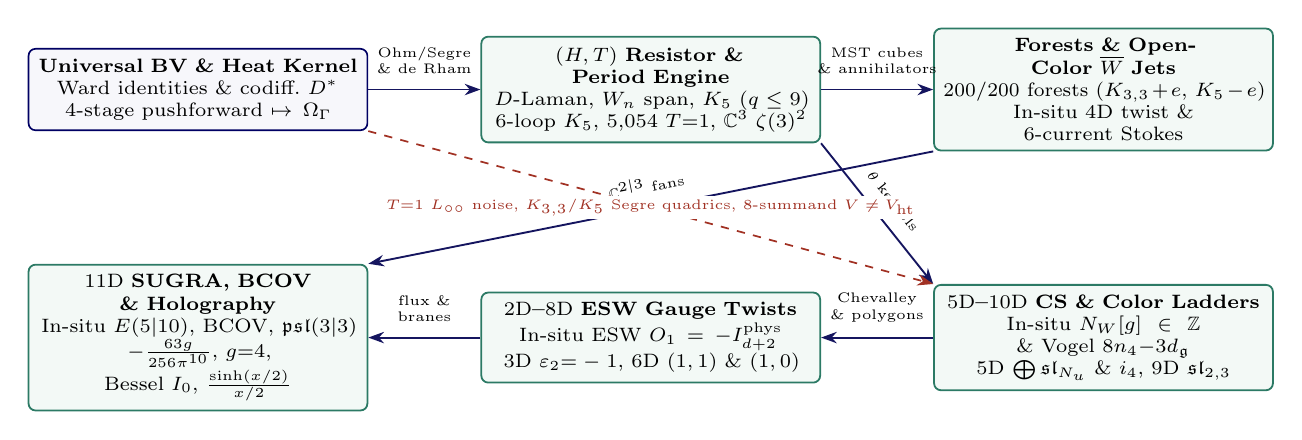
\begin{tikzpicture}[
  box/.style={draw=NavyBlue!78!black, line width=0.6pt, rounded corners=2.5pt, fill=NavyBlue!3, align=center, font=\scriptsize, inner sep=3.6pt},
  res/.style={draw=PineGreen!80!black, line width=0.65pt, rounded corners=2.5pt, fill=PineGreen!4, align=center, font=\scriptsize, inner sep=3.6pt},
  good/.style={-{Stealth[length=2.0mm,width=1.45mm]}, line width=0.68pt, draw=MidnightBlue!85!black},
  bad/.style={-{Stealth[length=2.0mm,width=1.45mm]}, line width=0.62pt, dashed, draw=BrickRed!85!black}
]
  \node[box, text width=4.05cm] (found) at (0, 3.15) {\textbf{Universal BV \& Heat Kernel}\\Ward identities \& codiff.\ $D^*$\\$4$-stage pushforward $\mapsto\Omega_\Gamma$};
  \node[res, text width=4.05cm] (net) at (5.75, 3.15) {\textbf{$(H,T)$ Resistor \& Period Engine}\\$D$-Laman, $W_n$ span, $K_5$ ($q\le 9$)\\$6$-loop $K_5$, $5{,}054$ $T{=}1$, $\C^3$ $\zeta(3)^2$};
  \node[res, text width=4.05cm] (for) at (11.50, 3.15) {\textbf{Forests \& Open-Color $\Wb$ Jets}\\$200/200$ forests ($K_{3,3}+e$, $K_5-e$)\\In-situ $4\mathrm{D}$ twist \& $6$-current Stokes};

  \node[res, text width=4.05cm] (holo) at (0, 0) {\textbf{$11\mathrm{D}$ SUGRA, BCOV \& Holography}\\In-situ $E(5|10)$, BCOV, $\fpsl(3|3)$\\$-\frac{63g}{256\pi^{10}}$, $g{=}4$, Bessel $I_0$, $\frac{\sinh(x/2)}{x/2}$};
  \node[res, text width=4.05cm] (gauge) at (5.75, 0) {\textbf{$2\mathrm{D}$--$8\mathrm{D}$ ESW Gauge Twists}\\In-situ ESW $O_1=-I^{\mathrm{phys}}_{d+2}$\\$3\mathrm{D}$ $\eps_2{=}-1$, $6\mathrm{D}$ $(1,1)$ \& $(1,0)$};
  \node[res, text width=4.05cm] (cs) at (11.50, 0) {\textbf{$5\mathrm{D}$--$10\mathrm{D}$ CS \& Color Ladders}\\In-situ $N_W[g]\in\ZZ$ \& Vogel $8n_4{-}3d_{\fg}$\\$5\mathrm{D}$ $\bigoplus\fsl_{N_u}$ \& $i_4$, $9\mathrm{D}$ $\fsl_{2,3}$};

  \draw[good] (found) -- node[above=2pt, font=\tiny, align=center] {Ohm/Segre\\\& de~Rham} (net);
  \draw[good] (net) -- node[above=2pt, font=\tiny, align=center] {MST cubes\\\& annihilators} (for);
  \draw[good] (net.south east) -- node[above=2pt, sloped, font=\tiny] {$\theta$ kernels} (cs.north west);
  \draw[good] (cs) -- node[above=2pt, font=\tiny, align=center] {Chevalley\\\& polygons} (gauge);
  \draw[good] (gauge) -- node[above=2pt, font=\tiny, align=center] {flux \&\\branes} (holo);
  \draw[good] (for.south west) -- node[above=2pt, sloped, font=\tiny] {$\C^{2|3}$ fans} (holo.north east);

  \draw[bad] (found.south east) -- node[fill=white, inner sep=1.2pt, font=\tiny, text=BrickRed!85!black] {$T{=}1$ $L_{\circ\circ}$ noise, $K_{3,3}/K_5$ Segre quadrics, $8$-summand $V\neq V_{\mathrm{ht}}$} (cs.north west);
\end{tikzpicture}
\caption{Proximity-ordered logical architecture of this lecture monograph: universal Ward/BV heat-kernel foundations lead directly into the multi-loop $(H,T)$ resistor-network, period, and forest engines, while sector-specific Background Cards ($4\mathrm{D}$ off-shell twist, Chern--Simons $N_W[g]\in\ZZ$, Whitehead--Vogel color ladders, ESW taxonomy, $11\mathrm{D}$ pure spinors, BCOV, and $\fpsl(3|3)$) enter in situ right where each physical calculation invokes them.}
\label{fig:overview}
\end{figure}

Following the proximity principle---building universal foundations once upfront and placing concrete algebraic or geometric background cards directly adjacent to the Feynman-diagram calculations that invoke them---the monograph is organized into eight chapters and two reference appendices. Section~\ref{sec:summary-ledger} establishes the global typed index variance ledger (`Background Card~2.1`), the electrical Kirchhoff/Ohm cycle forms, and a self-contained catalogue of all principal theorems. Section~\ref{sec:ward-bv-primer} constructs the universal Euclidean Ward-identity and graded BV foundation (`Background Card~3.1`) and derives the master $(H,T)$ resistor-network form $\Omega_\Gamma$ directly from Costello's codifferential heat-kernel parametrix. Immediately entering multi-loop integration, Section~\ref{sec:schwinger-periods-k5} proves $(H,T)$ $D$-Laman admissibility, closed two-loop theta kernels, $T\ge 2$ Pfaffian loop vanishing, Ohm/Segre locality, fixed-core wheel stabilization, non-planar $K_5$ reduction through six loops and $q=9$, $5{,}054$ half-integer $T=1$ periods, three-terminal locality, and five-loop $\C^3$ kernels.

Section~\ref{sec:forests-quartic-jets} develops universal sourced-forest elimination, $19$-loop paired-star and $128$-loop fan reduction, and the five-loop $K_{3,3}+e$ and $200/200$ forest census, then introduces the off-shell four-dimensional $\mathcal{N}=1$ and $\mathcal{N}=4$ twist card in situ to prove universal open-color $\zeta(3)$ cancellation and closed six-current simplex jet reduction. Section~\ref{sec:cs-gauge-twists} introduces Chern--Simons transgression, exact Wess--Zumino winding $N_W[g]\in\ZZ$, and superconnections in situ, evaluates the two-loop $5\mathrm{D}$ Chern--Simons theta graphs, introduces the Whitehead and Vogel split-Casimir background cards (with complete proofs of $C_2(V\otimes W)$, semisimple vs.\ simple $X_2$ splitting, and Vogel's dimension and Möbius-trace formulas) right at the Lie color contraction step to classify $5\mathrm{D}$, $9\mathrm{D}$, and $10\mathrm{D}$ Chern--Simons theories, and places the Elliott--Safronov--Williams taxonomy card right ahead of multi-loop $2\mathrm{D}$--$8\mathrm{D}$ gauge twists. Section~\ref{sec:sugra-bcov-holo} introduces pure-spinor $11\mathrm{D}$ supergravity, Calabi--Yau BCOV gravity, and $\fpsl(3|3)$ super-polyvector cards immediately ahead of the two-loop $11\mathrm{D}$ obstruction, four-loop BCOV invariants, and all-order $\mathcal{N}=4$ twisted holography. Finally, Section~\ref{sec:conclusion} presents a turnkey four-step practitioner recipe, open frontiers, and five-paper roadmap, supported by Appendices~\ref{app:conventions} and~\ref{app:periods-errata}.

% ============================================================================
\section{Typed Index Variance Ledger and Catalogue of Principal Theorems}
\label{sec:summary-ledger}
% ============================================================================

Before entering the perturbative derivations, we codify our global index-variance contract (`Background Card~2.1`, synchronized with \zkmat) and assemble a self-contained reference ledger of the principal theorems proved across Sections~\ref{sec:ward-bv-primer}--\ref{sec:sugra-bcov-holo}.

\subsection{Typed Abstract and Component Index Variance Ledger}
\label{subsec:notation-ledger}

\begin{zkmodule}{Global Typed Abstract and Component Index Variance Ledger}{typed-index-variance-ledger}
Let $\mathcal{V} \cong \C^H$ denote the model holomorphic tangent vector space of $X = \RR^T \times \C^H$ ($D := H + T$), with complex-linear dual $\mathcal{V}^* := \Hom_{\C}(\mathcal{V}, \C)$ and complex-conjugate space $\overline{\mathcal{V}}$. In general $(H,T)$ chapters, lowercase Latin letters $\mathsf{a},\mathsf{b},\mathsf{c}$ (or $a,b,c$ when four-dimensional Weyl spinors are absent; in four-dimensional spinorial formulas, $a,b \in \{+,-\}$ and $\dot{a},\dot{b} \in \{\dot{+},\dot{-}\}$ denote chiral and antichiral $\Spin(4)$ Weyl spinor slots as detailed in Appendix~\ref{app:conventions}) denote basis-independent abstract tensor slots on $\mathcal{V}$ and $\mathcal{V}^*$ ($v^{\mathsf{a}} \in \mathcal{V}$, $w_{\mathsf{a}} \in \mathcal{V}^*$, canonical evaluation $w_{\mathsf{a}}v^{\mathsf{a}} \in \C$, identity endomorphism $\delta^{\mathsf{a}}{}_{\mathsf{b}} \in \mathcal{V}\otimes\mathcal{V}^*$). Fixing a basis $(e_i)^{\mathsf{a}}$ of $\mathcal{V}$ and dual basis $(e^i)_{\mathsf{a}}$ of $\mathcal{V}^*$ indexed by $i,j \in \{1,\dots,H\}$ gives
\begin{equation}
\label{eq:tetrad-bridge}
(e_i)^{\mathsf{a}}(e^j)_{\mathsf{a}} = \delta_i{}^j,\qquad
(e_i)^{\mathsf{a}}(e^i)_{\mathsf{b}} = \delta^{\mathsf{a}}{}_{\mathsf{b}},\qquad
v^{\mathsf{a}} = v^i(e_i)^{\mathsf{a}},\qquad
w_{\mathsf{a}} = w_i(e^i)_{\mathsf{a}},
\end{equation}
where repeated opposite-variance component indices contract by Einstein summation over $\{1,\dots,H\}$. Complex conjugation maps $v^i \mapsto \bar{v}^{\bar{\imath}} \in \overline{\mathcal{V}}$ at the identical upper height; pairing $\mathcal{V}$ with $\overline{\mathcal{V}}$ always inserts the flat K\"ahler metric $\delta_{i\bar{\jmath}} \in \mathcal{V}^*\otimes\overline{\mathcal{V}}^*$ and its inverse $\delta^{\bar{\jmath}i}$.

Seven typed index families govern the field-theoretic, Lie-algebraic, spinorial, and electrical-network constructions across all chapters (Table~\ref{tab:variance-ledger} and Table~\ref{tab:zk-module-index}):
\begin{itemize}[leftmargin=*]
  \item \emph{Holomorphic chart indices} $i,j,k \in \{1,\dots,H\}$ and conjugate $\bar{\imath},\bar{\jmath} \in \{1,\dots,H\}$ on $\C^H$, alongside real topological coordinates $\tau^\rho$ ($\rho,\sigma \in \{1,\dots,T\}$; metric $\delta_{\rho\sigma}$) on $\RR^T$;
  \item \emph{Four-dimensional Euclidean spacetime, Weyl, and Weinberg--Srednicki spinor indices}: Lorentz $\mu,\nu \in \{0,1,2,3\}$ ($g_{\mu\nu} = \delta_{\mu\nu}$), chiral Weyl $a,b \in \{+,-\}$, antichiral Weyl $\dot{a},\dot{b} \in \{\dot{+},\dot{-}\}$ (bispinor $x^{a\dot{a}} = x^\mu(\bar{\sigma}_\mu)^{\dot{a}a}$), and four-component Majorana $\alpha,\beta \in \{1,2,3,4\}$ ($\bar{\lambda}^{\alpha A} := \lambda_\beta{}^A C^{\beta\alpha}$);
  \item \emph{Lie-algebra slots} $A,B,C,E$ on $\fg$ and $\fg^*$ ($d_{\fg} := \dim_{\C}\fg$; omitting $D$ to avoid collision with $D = H+T$ and auxiliary $D^A$), with invariant bilinear form $\kappa_{AB} \in \Sym^2(\fg^*)^{\fg}$, inverse $\kappa^{AB}$, and structure constants $[t_B, t_C] = \ii C^A{}_{BC}t_A$ (or complex basis $[T_B, T_C] = f^A{}_{BC}T_A$ with $f_{ABC} := \kappa_{AE}f^E{}_{BC}$);
  \item \emph{Matter representation indices} $I,J,K \in \{1,\dots,\dim\cR\}$ on $\cR$ ($\phi^I, \psi_a{}^I, F^I, \beta^I \in \cR$) and dual $\cR^*$ ($\bar{\phi}_I, \bar{\psi}_{\dot{a}I}, \bar{F}_I, \gamma_I \in \cR^*$);
  \item \emph{Superspace Grassmann indices} $\hat{\alpha},\hat{\beta} \in \{1,\dots,N_{\theta}\}$ for odd coordinates $\theta^{\hat{\alpha}}$ and derivatives $\partial_{\hat{\alpha}}$ on $\C^{H|N_{\theta}}$;
  \item \emph{Typed Schwinger electrical-network spaces and holomorphic cycle $1$-forms $\psi_{r,\mathsf{a}}$}: For a connected oriented graph $\Gamma = (V,I)$ with $|V|$ vertices, $|I|$ internal edges, loop number $n := |I| - |V| + 1 \ge 1$, and grounded root vertex $v_0 \in V$, we distinguish the edge space $\mathcal{E} := \RR^{|I|}$ ($e,f \in \{1,\dots,|I|\}$), grounded vertex space $\mathcal{W}_{\mathrm{vert}} := \RR^{|V|-1}$ ($u,v \in \{1,\dots,|V|-1\}$), and cycle space $\mathcal{H}_1 := H_1(\Gamma;\RR) \cong \RR^n$ ($r,s \in \{1,\dots,n\}$). Assigning each edge $e$ its Schwinger proper time as resistance $R_{ef}(t) := t_e\delta_{ef}$ (conductance $G^{ef}(t) := t_e^{-1}\delta^{ef}$), the incidence map $B^u{}_e : \mathcal{E} \to \mathcal{W}_{\mathrm{vert}}$ and cycle-selection map $C_r{}^e : \mathcal{E}^* \to \mathcal{H}_1^*$ ($B^u{}_e C_r{}^f\delta^{eg}\delta_{fg} = 0$) define the grounded nodal Laplacian $\Lambda^{uv}(t) := B^u{}_e G^{ef}(t) B^v{}_f$ and loop-resistance Symanzik matrix $M_{rs}(t) := C_r{}^e R_{ef}(t) C_s{}^f$ ($U_\Gamma(t) := \det M(t)$). Injecting balanced external holomorphic momenta $\lambda^u{}_{\mathsf{a}} \in \mathcal{W}_{\mathrm{vert}}\otimes\mathcal{V}^*$ drives potential drops $\varphi_{u,\mathsf{a}} = (\Lambda^{-1})_{uv}\lambda^v{}_{\mathsf{a}}$ and Ohm edge currents $y^e{}_{\mathsf{a}}(t;\lambda) := G^{ef}B^u{}_f(\Lambda^{-1})_{uv}\lambda^v{}_{\mathsf{a}}$ obeying Kirchhoff's current law $B^u{}_e y^e{}_{\mathsf{a}} = \lambda^u{}_{\mathsf{a}}$ and voltage law $C_r{}^e R_{ef} y^f{}_{\mathsf{a}} = 0$. Pairing the resistance differentials $\dd t^e \in \Omega^1(\RR^{|I|}_{>0};\mathcal{E})$ against $y^f{}_{\mathsf{a}}$ along cycle $r$ defines the \emph{holomorphic cycle $1$-form}
  \begin{equation}
  \label{eq:psi-cycle-def}
  \psi_{r,\mathsf{a}} := C_r{}^e R_{ef}'\,y^f{}_{\mathsf{a}}\,\dd t^e = \sum_{\substack{e \in I\\\mathrm{edges\ in\ }r}} C_r{}^e\,y^e{}_{\mathsf{a}}(t;\lambda)\,\dd t^e \in \Omega^1\!\bigl(\RR^{|I|}_{>0}\bigr)\otimes\mathcal{H}_1^*\otimes\mathcal{V}^*,
  \end{equation}
  whose radial contraction $\iota_E\psi_{r,\mathsf{a}} = C_r{}^e R_{ef} y^f{}_{\mathsf{a}} = 0$ along $E = \sum_{\substack{e\in I\\\mathrm{edges}}} t^e\partial_{t^e}$ vanishes identically by Kirchhoff's voltage law, ensuring descent to projective Schwinger space $\mathbb{RP}^{|I|-1}_{>0}$! Moreover, partitioning any subnetwork $S \subset \Gamma$ into boundary terminals $\partial S$ and eliminated interior vertices $S^\circ$ splits its conductance Laplacian into $L_{\partial\partial}, L_{\partial\circ}, L_{\circ\partial}$, and the positive-definite $|S^\circ|\times|S^\circ|$ \emph{interior Dirichlet conductance Laplacian}
  \begin{equation}
  \label{eq:Lcirc-ledger-def}
  (L_{\circ\circ})^{uv} := \left(\sum_{\substack{e\in I(S)\\ e\ni u}} g_e\right)\delta^{uv} - \sum_{\substack{e\in I(S)\\ e=(u,v)}} g_e\qquad (u,v \in S^\circ,\ g_e := t_e^{-1}).
  \end{equation}
\end{itemize}
\end{zkmodule}

\begin{table}[H]
\centering
\scriptsize
\setlength{\tabcolsep}{3.4pt}
\renewcommand{\arraystretch}{1.16}
\begin{tabularx}{\textwidth}{@{}ll>{\raggedright\arraybackslash}X>{\raggedright\arraybackslash}X@{}}
\toprule
\textbf{Index Family} & \textbf{Carrier Space / Bundle} & \textbf{Contravariant (Upper) Objects} & \textbf{Covariant (Lower) Objects} \\
\midrule
$\mathsf{a},\mathsf{b},\mathsf{c}$ & Abstract $\mathcal{V} \cong \C^H$ vs.\ $\mathcal{V}^*$ & $z^{\mathsf{a}}, \mu^{\mathsf{a}}, (e_i)^{\mathsf{a}}$ & $p_{\mathsf{a}}, \lambda^u{}_{\mathsf{a}}, y^e{}_{\mathsf{a}}, \psi_{r,\mathsf{a}}, (e^i)_{\mathsf{a}}$ \\
$i,j;\ \bar{\imath},\bar{\jmath} \in \{1..H\}$ & $\C^H$ chart \& conjugate $\overline{\mathcal{V}}$ & $z^i, \bar{z}^{\bar{\imath}}, \mu^i, \delta^{\bar{\jmath}i}, \eps^{i_1\cdots i_H}$ & $\partial_i, \dbar_{\bar{\imath}}, \gamma_i, \delta_{i\bar{\jmath}}, \eps_{i_1\cdots i_H}$ \\
$\mu,\nu;\ a,\dot{a};\ \alpha,\beta$ & $4\mathrm{D}$ $\RR^4$, Weyl $S_\pm$, Majorana & $x^\mu, x^{a\dot{a}}, \xi^a, \bar{\lambda}^{\dot{a}A}, \bar{\lambda}^{\alpha A}, C^{\alpha\beta}$ & $\partial_\mu, V_\mu{}^A, \lambda_a{}^A, \bar{\lambda}_{\dot{a}}{}^A, \lambda_\alpha{}^A, C_{\alpha\beta}$ \\
$A,B,C,E$ & Lie algebra $\fg$ vs.\ dual $\fg^*$ & $\mathcal{A}^A, V_\mu{}^A, \ghc^A, \kappa^{AB}, C^A{}_{BC}$ & $\mathcal{B}_A, \ghb_A, A^\ddagger_A, \ghc^\ddagger_A, \kappa_{AB}, f_{ABC}$ \\
$I,J,K \in \{1..\dim\cR\}$ & Matter module $\cR$ vs.\ $\cR^*$ & $\phi^I, \psi_a{}^I, F^I, \beta^I, \bar{F}^{\ddagger I}, \Wb^{IJK}$ & $\bar{\phi}_I, \bar{\psi}_{\dot{a}I}, \bar{F}_I, \gamma_I, \phi^\ddagger_I, W_{IJK}$ \\
$e,f \in \{1..|I|\}$ & Schwinger edge space $\mathcal{E}$ & $t^e, \dd t^e, y^e{}_{\mathsf{a}}, G^{ef}$ & $z_e{}^{\mathsf{a}}, R_{ef}, B^u{}_e$ \\
$u,v;\ r,s$ & Grounded $\mathcal{W}_{\mathrm{vert}}$; cycles $\mathcal{H}_1$ & $\lambda^u{}_{\mathsf{a}}, \Lambda^{uv}, (L_{\circ\circ})^{uv}, (M^{-1})^{rs}$ & $\varphi_{u,\mathsf{a}}, (\Lambda^{-1})_{uv}, M_{rs}, C_r{}^e, \psi_{r,\mathsf{a}}$ \\
\bottomrule
\end{tabularx}
\caption{Global typed index variance ledger enforced across all derivations, Feynman diagrams, and in-situ Background Cards.}
\label{tab:variance-ledger}
\end{table}

\begin{table}[H]
\centering
\scriptsize
\setlength{\tabcolsep}{3.5pt}
\renewcommand{\arraystretch}{1.15}
\begin{tabularx}{\textwidth}{@{}ll>{\raggedright\arraybackslash}X@{}}
\toprule
\textbf{In-Situ Background Card} & \textbf{Zettelkasten Link} & \textbf{Adjacent Calculation Motivating Placement (Proximity Principle)} \\
\midrule
Card~2.1 (\S\ref{subsec:notation-ledger}) & \zkcard{typed-index-variance-ledger} & Global index variance, Kirchhoff/Ohm $\psi_{r,\mathsf{a}}$, and $L_{\circ\circ}$ across all chapters \\
Card~3.1 (\S\ref{subsec:bv-graded-module}) & \zkcard{bv-linfty-physics-grading} & Universal BV grading, codifferential $D^*$, and $4$-stage derivation of $\Omega_\Gamma$ \\
Card~5.1 (\S\ref{subsec:universal-quartic-product}) & \zkcard{offshell-n1-bv-master-action} & Off-shell $4\mathrm{D}$ $\mathcal{N}=1,4 \to BF$--$\beta\gamma$ / $\C^{2|3}$ hCS right before open-color $\Wb$ products \\
Card~6.1 (\S\ref{subsec:cs-aksz-lecture}) & \zkcard{aksz-superconnection-ht-cs-ladder} & $\mathrm{CS}_{3,5}$, exact $N_W[g]\in\ZZ$, AKSZ, \& $-3F_D$ right before $5\mathrm{D}$--$10\mathrm{D}$ CS loops \\
Card~6.2 (\S\ref{subsec:5d-cs-flagship}) & \zkcard{low-rank-isomorphisms-cubic-invariants} & Chevalley Casimirs \& Whitehead $H^3(\fg;\C)$ right at $5\mathrm{D}$ CS two-loop color step \\
Card~6.3 (\S\ref{subsec:5d-cs-flagship}) & \zkcard{vogel-universal-plane} & Split Casimir $m_k,n_k$, $X_2$, \& Vogel $8n_4-3d_{\fg}$ right at $5\mathrm{D}$ CS $\theta$-graph contraction \\
Card~6.4 (\S\ref{subsec:esw-taxonomy}) & \zkcard{esw-twist-taxonomy-oneloop-anomaly-table} & ESW $10\mathrm{D}\to 2\mathrm{D}$ twist classes \& $O_1 = -I^{\mathrm{phys}}_{d+2}$ right before $2\mathrm{D}$--$8\mathrm{D}$ gauge twists \\
Card~7.1 (\S\ref{subsec:11d-two-loop}) & \zkcard{minimal-11d-sugra-e510-model} & Pure-spinor $11\mathrm{D}$ CJS SUGRA $\to E(5|10)$ right before $11\mathrm{D}$ two-loop theta sum \\
Card~7.2 (\S\ref{subsec:ks-type1-bcov}) & \zkcard{ks-type1-wzw4-minimal-bcov} & Calabi--Yau $\partial_\Omega$, $P_{\mathrm{BCOV}}$, \& $\mathrm{D}3$ flux $NF_{\mathrm{BM}}$ right before $4$-loop KS \& $g=4$ BCOV \\
Card~7.3 (\S\ref{subsec:holography-allorder}) & \zkcard{chang-yin-superfield-letters} & Super-polyvectors $\mathrm{PV}^{\ge 1}_\Delta(\C^{2|3})$ \& $\fpsl(3|3)$ right before $\mathcal{N}=4$ twisted holography \\
\bottomrule
\end{tabularx}
\caption{In-situ Background Cards placed directly alongside the Feynman-diagram and cohomology calculations that require them, synchronized bidirectionally with the local Ospero Zettelkasten (\texttt{http://127.0.0.1:9124/}).}
\label{tab:zk-module-index}
\end{table}

\begin{figure}[H]
\centering
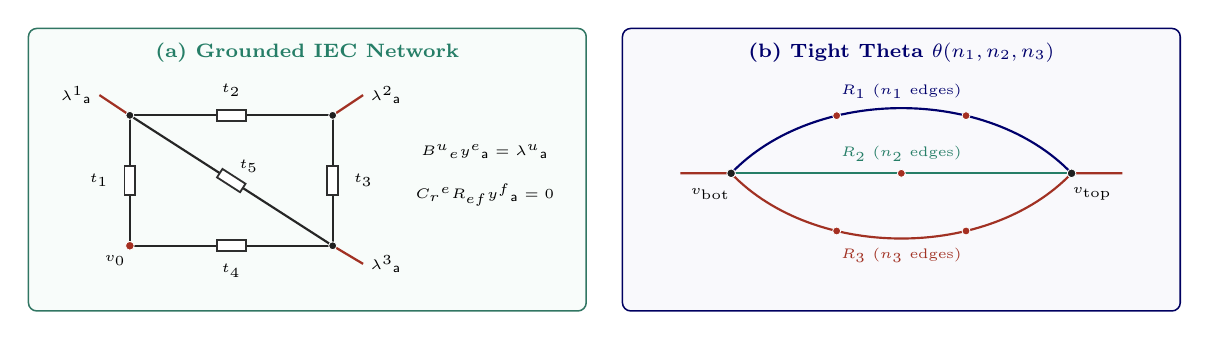
\begin{tikzpicture}[scale=0.92]
  % Left: Grounded IEC resistor network
  \begin{scope}[shift={(-4.10,0)}]
    \draw[rounded corners=3pt, draw=PineGreen!75!black, fill=PineGreen!2.5, line width=0.55pt] (-3.85,-1.95) rectangle (3.85,1.95);
    \node[font=\scriptsize\bfseries, text=PineGreen!85!black] at (0,1.62) {(a) Grounded IEC Network};
    \coordinate (g0) at (-2.45,-1.05);
    \coordinate (g1) at (-2.45, 0.75);
    \coordinate (g2) at ( 0.35, 0.75);
    \coordinate (g3) at ( 0.35,-1.05);
    \draw[prop] (g0) -- node[iecres, rotate=90, scale=0.62] {} node[left=4pt, font=\tiny] {$t_1$} (g1);
    \draw[prop] (g1) -- node[iecres, scale=0.62] {} node[above=3pt, font=\tiny] {$t_2$} (g2);
    \draw[prop] (g2) -- node[iecres, rotate=90, scale=0.62] {} node[right=4pt, font=\tiny] {$t_3$} (g3);
    \draw[prop] (g0) -- node[iecres, scale=0.62] {} node[below=3pt, font=\tiny] {$t_4$} (g3);
    \draw[prop] (g1) -- node[iecres, sloped, scale=0.58] {} node[above right=-1pt, font=\tiny] {$t_5$} (g3);
    \draw[extleg] (g1) -- ++(-0.42,0.28) node[left=-1pt, font=\tiny] {$\lambda^1{}_{\mathsf{a}}$};
    \draw[extleg] (g2) -- ++( 0.42,0.28) node[right=-1pt, font=\tiny] {$\lambda^2{}_{\mathsf{a}}$};
    \draw[extleg] (g3) -- ++( 0.42,-0.25) node[right=-1pt, font=\tiny] {$\lambda^3{}_{\mathsf{a}}$};
    \filldraw[v0] (g1) circle (0.055cm);
    \filldraw[v0] (g2) circle (0.055cm);
    \filldraw[v0] (g3) circle (0.055cm);
    \filldraw[vbiv] (g0) circle (0.06cm) node[below left=1pt, font=\tiny] {$v_0$};
    \node[font=\tiny] at (2.45, 0.25) {$B^u{}_e y^e{}_{\mathsf{a}} = \lambda^u{}_{\mathsf{a}}$};
    \node[font=\tiny] at (2.45,-0.35) {$C_r{}^e R_{ef} y^f{}_{\mathsf{a}} = 0$};
  \end{scope}

  % Right: Two-loop tight theta graph \theta(n_1,n_2,n_3)
  \begin{scope}[shift={(4.10,0)}]
    \draw[rounded corners=3pt, draw=NavyBlue!75!black, fill=NavyBlue!2.5, line width=0.55pt] (-3.85,-1.95) rectangle (3.85,1.95);
    \node[font=\scriptsize\bfseries, text=NavyBlue!85!black] at (0,1.62) {(b) Tight Theta $\theta(n_1,n_2,n_3)$};
    \coordinate (VL) at (-2.35,-0.05);
    \coordinate (VR) at ( 2.35,-0.05);
    \draw[prop, NavyBlue!85!black] (VL) .. controls (-1.20,1.15) and (1.20,1.15) .. coordinate[pos=0.33] (p1a) coordinate[pos=0.67] (p1b) (VR);
    \draw[prop, PineGreen!85!black] (VL) -- coordinate[pos=0.50] (p2a) (VR);
    \draw[prop, BrickRed!85!black] (VL) .. controls (-1.20,-1.25) and (1.20,-1.25) .. coordinate[pos=0.33] (p3a) coordinate[pos=0.67] (p3b) (VR);
    \foreach \pt in {p1a,p1b,p2a,p3a,p3b} \filldraw[vbiv] (\pt) circle (0.055cm);
    \draw[extleg] (-3.05,-0.05) -- (VL);
    \draw[extleg] (VR) -- (3.05,-0.05);
    \filldraw[v0] (VL) circle (0.06cm) node[below left=1pt, font=\tiny] {$v_{\mathrm{bot}}$};
    \filldraw[v0] (VR) circle (0.06cm) node[below right=1pt, font=\tiny] {$v_{\mathrm{top}}$};
    \node[font=\tiny, text=NavyBlue!85!black] at (0,1.08) {$R_1$ ($n_1$ edges)};
    \node[font=\tiny, text=PineGreen!85!black] at (0,0.22) {$R_2$ ($n_2$ edges)};
    \node[font=\tiny, text=BrickRed!85!black] at (0,-1.18) {$R_3$ ($n_3$ edges)};
  \end{scope}
\end{tikzpicture}
\caption{Fundamental Schwinger electrical-network structures from Background Card~2.1: (a)~grounded IEC white-rectangle resistor network with root $v_0$, external vertex currents $\lambda^u{}_{\mathsf{a}}$, Kirchhoff current law $B^u{}_e y^e{}_{\mathsf{a}} = \lambda^u{}_{\mathsf{a}}$, and cycle voltage law $C_r{}^e R_{ef} y^f{}_{\mathsf{a}} = 0$ generating $\psi_{r,\mathsf{a}}$~\eqref{eq:psi-cycle-def}; (b)~two-loop tight theta topology $\theta(n_1,n_2,n_3)$ ($n_1+n_2+n_3 = 2D+1$, $1 \le n_P \le D$) with trivalent poles $v_{\mathrm{bot}}, v_{\mathrm{top}}$ and red bivalent source insertions.}
\label{fig:iec-and-theta}
\end{figure}

\subsection{Self-Contained Catalogue of Principal Theorems}
\label{subsec:catalogue-results}

\begin{enumerate}[label=\textbf{Result~\arabic*.},leftmargin=*]
  \item \textbf{Four-Stage Heat-Kernel Resistor-Network Derivation, $D$-Laman Admissibility, and $\mathrm{B}\supsetneq\mathrm{SP}$ (Theorems~\ref{thm:heat-kernel-omega-gamma} and~\ref{thm:d-laman}).} Integrating Costello's heat-kernel propagator $P(\eps,L) = \int_\eps^L\dd t\,D^* K_t$ across the $|V|-1$ ungrounded vertices of an $n$-loop graph on $\RR^T\times\C^H$ yields $\Omega_\Gamma = U_\Gamma^{-H}\rho_n(M)^{\wedge T}\wedge\bigwedge_{i=1}^H\bigwedge_{r=1}^n\psi_{r,i}$. Tight UV-convergent graphs obey $|I| = Dn+1$, $|V| = (D-1)n+2$, and $(D-1)|I_S| \le D|V_S|-D-1$, with unsourced star--triangle class $\mathrm{B}$ strictly larger than $\mathrm{SP}$ for every $D \ge 3, n \ge 3$.

  \item \textbf{Universal Two-Loop Theta Kernels, $T\ge 2$ Vanishing, and Ohm/Segre Locality (Theorems~\ref{thm:theta-closed}--\ref{thm:ohm-locality}).} Closed determinants evaluate all tight $\theta(n_1,n_2,n_3)$ kernels at $T\in\{0,1\}$; Newton's identities prove $\rho_n(M)\wedge\rho_n(M) = 0$ (eliminating all bulk loops for $T \ge 2$); and Schur complementation proves $\Omega_\Gamma = \eps\,\Omega_S\wedge(\Omega_{\mathrm{out}}\circ p_{\mathrm{out}})$ with $T=1$ Dirichlet contact $\langle\xi_u\xi_v\rangle = \frac{1}{2}(L_{\circ\circ})_{uv}$ and codimension-$\frac{1}{2}k(k-3)$ Segre quadrics at valence $k \ge 4$.

  \item \textbf{Fixed-Core de~Rham Stabilization and Sharp $n$-Spoke Wheel Span (Theorems~\ref{thm:core-stabilization} and~\ref{thm:wheel-span}).} Relative algebraic de~Rham cohomology on Hepp cubes proves $\dim_{\QQ}\bigcup_{r\ge 1}\mathcal{P}_r(G) < \infty$ and $\mathcal{P}_q(G) = \mathcal{P}_{q+1}(G)$ ($q\gg 1$), while bilateral Laplace parity and the factorial bound $L_{21} > \frac{5}{4} > \zeta(3)$ prove $\mathcal{P}_q(W_n) = \QQ + \sum_{\substack{j\in\{2,\dots,n-1\}\\\mathrm{odd\ zetas}}}\QQ\zeta(2j-1)$ for all $n \ge 3$ and $q \ge \max(3,n-1)$ without assuming $\QQ$-independence of odd zetas.

  \item \textbf{Non-Planar $K_5$ Closure Through $q=9$ and All Three Six-Loop $\C^2$ Kernels (Theorems~\ref{thm:k5-periods} and~\ref{thm:sixloop-k5}).} Vertex IBP plus dimension shift closes all convergent $K_5$ orbits for $q \le 8$ ($54{,}391$ orbits) and all $73$ Wishart/Cayley--Menger guarded $q=9$ orbits in $\QQ + \QQ\zeta(3) + \QQ\zeta(5)$ (with radial-wheel proof of $J_2 = 4J_3^{(14)}+16J_3^{(6)}+\frac{16}{3}J_3^{(5)}$), and reciprocal conductance inversion ($35 \to 15$) evaluates all three admissible six-loop $\C^2$ $K_5$ subdivisions.

  \item \textbf{$T=1$ Four-Loop $5{,}054$-Period Completion, $3$-Terminal Locality, and $5$-Loop $\C^3$ $\zeta(3)^2$ (Theorems~\ref{thm:t1-completion} and~\ref{thm:bulk3-five-loop}).} Closing $55{,}074$ IBP rows determines $5{,}054$ half-integer prism/$K_{3,3}$ periods in $\QQ\pi^2\oplus\QQ\pi^4$ ($K_{K_{3,3}}\equiv 0$ by degree-$6$ Vandermonde parity while edge $03$ current equals $\frac{2243\pi^2}{4725}-\frac{121\pi^4}{2520}$), three-terminal Markov truncation ($\alpha_{r_1}\wedge\alpha_{r_2}\wedge\alpha_{r_3}=0$) gives $K_{\mathrm{prism}}(1,1,0,-1,0,-1) = \frac{311}{630}\pi^2 - \frac{17}{360}\pi^4$, and $92$ five-loop $\C^3$ bare polynomials include $K_{62} = \frac{2804909}{1866590853120} - \frac{9019\zeta(3)}{3600676800} + \frac{29\zeta(3)^2}{27783000}$.

  \item \textbf{Universal Forest Elimination, Cube Series, $5$-Loop $K_{3,3}+e$, and $200/200$ Census (Theorems~\ref{thm:forest-cube-series}--\ref{thm:k33e-completion}).} Post-order elimination ($\le 3$ neighbors on $1{,}135$ forests), $\tau_\Gamma n!$ MST cubes with $(2n+1)\times(2n+1)$ determinant drop $4n \to 2n+1$, $19$-loop paired-star Schur reduction, $128$-loop spoke transfer, and $17$ parametric annihilators evaluate $K_{K_{3,3}+e}(1,0;2,1;-3,-1) = \frac{1187-816\zeta(3)}{435456000} > 0$, completing all $200/200$ five-loop $\C^2$ forests and the $468$-monomial $K_5-e$ current polynomial.

  \item \textbf{Off-Shell $4\mathrm{D}$ $\mathcal{N}=1,4$ Twists, Universal Open-Color $\zeta(3)$ Cancellation, $4$-Loop $\ghb^2$, and $6$-Current Jets (Proposition~\ref{prop:4d-offshell-twist}, Theorems~\ref{thm:universal-quartic} and~\ref{thm:simplex-jets}).} Eliminating $Q_-$-contractible pairs in off-shell $4\mathrm{D}$ $\mathcal{N}=1$ gauge-matter theory yields holomorphic $BF$--$\beta\gamma$ on $\C^2$ (and $\C^{2|3}$ hCS at $\mathcal{N}=4$), in which representation commutators $[t_A,t_B] - \ii C^C{}_{AB}t_C \equiv 0$ cancel $\zeta(3)$ identically for all pure-matter $\deg\Wb \ge 3$, across the $324$-matching four-loop $\ghb^2$ product, and across all simultaneous input derivative jets via the closed $6$-form $\omega_{F_q} = F_q(J)\,\dd^2 J_{WA}\wedge\dd^2 J_{WB}\wedge\dd^2 J_{AB}$ on $K_4$ ($46$ null $+ 16$ SP faces).

  \item \textbf{Exact Finite $\mathrm{CS}_3$ Gauge Shift, Winding $N_W[g] \in \ZZ$, AKSZ Collapse, and Vogel Identity $8n_4 - 3d_{\fg}$ (Propositions~\ref{prop:cs3-large-gauge-nw}--\ref{prop:casimir-x2-semisimple}, Theorem~\ref{thm:vogel-dim-and-8n4}).} Under $A^g = g A g^{-1} - (\dd g)g^{-1}$ ($\theta_g := g^{-1}\dd g$, matching $\delta_\epsilon A = -\dd_\nabla\epsilon$), $\frac{1}{2}\mathrm{CS}_3[A^g] - \frac{1}{2}\mathrm{CS}_3[A] = -\frac{1}{2}\dd\kappa(g A g^{-1},(\dd g)g^{-1}) + \frac{1}{12}\kappa(\theta_g,[\theta_g,\theta_g])$, integrating on closed $M_3$ to $4\pi^2 N_W[g]$ with $N_W[g] := \frac{1}{48\pi^2}\int_{M_3}\kappa^{\mathrm{norm}}(\theta_g,[\theta_g,\theta_g]) = \frac{1}{24\pi^2}\int_{M_3}\tr_{\C^N}((g^{-1}\dd g)^{\wedge 3}) \in \ZZ$ ($N_W[\id_{S^3}] = +1$), while right-placed antifields package $S_{E,\mathrm{BV}} = \frac{1}{2}\int_{M_3}\mathrm{CS}_3[\mathcal{A}]$ and $\int_{\RR\times\C^2}\mathrm{CS}_5[\mathcal{A}]|_{\mathrm{HT}} = -3F_D[\mathcal{A}]$. Semisimple $\fg$ splits $\Lambda^2\fg = \fg_{\mathrm{ad}}\oplus X_2$ with $\Omega_{\mathrm{ad}}|_{X_2} = 0$, whereas simple $\fg$ decomposes $\Sym^2\fg = \C\oplus\bigoplus_{\substack{s\in\{1,2,3\}\\\mathrm{branches}}}Y_2(v_s)$ ($\Omega_{\mathrm{ad}}|_{Y_2(v_s)} = -\frac{v_s}{2t_V}\id$) with $d_{\fg} = \frac{(v_1-2t_V)(v_2-2t_V)(v_3-2t_V)}{v_1 v_2 v_3}$ and $8n_4 - 3d_{\fg} = \frac{3d_{\fg}(d_{\fg}-3)v_1 v_2 v_3}{4t_V^3}$.

  \item \textbf{Commutative $5\mathrm{D}$, $9\mathrm{D}$, and $10\mathrm{D}$ Chern--Simons Classification (Lemma~\ref{lem:5d-cs-8summands}, Theorems~\ref{thm:5d-cs-allorders} and~\ref{thm:9d-10d-cs}).} Contraction invariance $\eta_v F = 0$ projects $8$-summand local functionals onto $H^g(V_{\mathrm{ht}})\cong H^{g+3}((C^0_{\fg})^G)$, where commutative $5\mathrm{D}$ CS quantizes on semisimple $\fg$ precisely when $\fg \cong \bigoplus_{\substack{u\\\mathrm{ideals}}}\fsl_{N_u}$ (with explicit $i_4 > 0$ and $\fg\oplus\C\mathbf{1}$ escape on $\fso_5\oplus\C\mathbf{1}$ and $G_2..E_8$), whereas $9\mathrm{D}$ HT CS quantizes $\mathrm{U}(4)$-equivariantly through $\hbar^2$ solely for $\fsl_2$ and $\fsl_3$ ($a = \pm\frac{1}{512\pi^4}$), and $10\mathrm{D}$ hCS satisfies $P_2 \mid P_6$ solely for $\{\fsl_2, \fso_5, \fso_{32}, E_8\}$.

  \item \textbf{$14$-Twist ESW One-Loop Match and Multi-Loop $3\mathrm{D}/4\mathrm{D}/6\mathrm{D}/8\mathrm{D}$ Gauge Supercharges (Theorems~\ref{thm:esw-oneloop}--\ref{thm:6d-8d-twistor}).} Across all $14$ ESW holomorphic twists, $(H+1)$-gon Berezinian supertraces satisfy $K_{\mathrm{poly}(H+1)} = \frac{(-1)^H}{H!}\Delta$ and $\mathcal{S}_H = -I^{\mathrm{phys}}_{d+2}$ ($38/38$ checks), accompanied by exact orientation $\eps_2 = -1$, $55$ four-loop tadpole moments, and $30{,}272$-monomial $\GL(2)+1\mathrm{F}$ $J_w=20$ lifts in $3\mathrm{D}$ $\mathcal{N}=2$, $4\mathrm{D}$ $\mathcal{N}=2$ $b_0$ lifts, $6\mathrm{D}$ $\mathcal{N}=(1,1)$ $Q_4$ and $\mathcal{N}=(1,0)$ rank-$5$ weights $(\frac{1}{2},\frac{1}{2},1,\frac{1}{2},\frac{1}{2})$, $6\mathrm{D}$ $\C^3$ $\fso_8$ GS, and all-loop twistor defect OPEs.

  \item \textbf{Pure-Spinor $11\mathrm{D}$ Supergravity, Delayed Genus-$4$ BCOV, and All-Order $\mathcal{N}=4$ Twisted Holography (Theorems~\ref{thm:11d-from-scratch}--\ref{thm:holography-allorder}).} Twisting $11\mathrm{D}$ CJS supergravity via $q = \mathbf{1} \in \Lambda^0 V^* \subset S_{32}$ yields $E(5|10)$ with two-loop obstruction $-\frac{63g}{256\pi^{10}}$ on $\mathcal{Z}_{3+6}$ and further-twist Koszul $g$-torsion; Kodaira--Spencer and minimal BCOV gravity yield $D_4 > 0$ and delayed $g=4$ response $\frac{31}{64012032000}$; and $\mathcal{N}=4$ twisted holography yields $\mathcal{O}(\hbar^2 N^{-2})$ $3\to 1$ trace fusion, Bessel $I_0$ detectors, $\frac{\sinh(x/2)}{x/2}$ handle limit, determinant branes, $k=2$ mesons, and $2J_L \ge 2n-1$ spin selection.
\end{enumerate}

% ============================================================================
\section{Universal Foundations: Euclidean Ward Identities, Graded BV Algebra, and the Heat-Kernel Resistor Form \texorpdfstring{$\Omega_\Gamma$}{Omega\_Gamma}}
\label{sec:ward-bv-primer}
% ============================================================================

Following the proximity principle, this chapter builds strictly the \textbf{universal foundation} required across every calculation in the monograph---Euclidean Ward--Takahashi identities, graded Batalin--Vilkovisky (BV) abstract indices, Costello's codifferential heat-kernel parametrix $P(\eps,L)$, and the four-stage Gaussian vertex derivation of the master $(H,T)$ electrical-network differential form $\Omega_\Gamma$---so that we enter multi-loop Feynman-diagram integration immediately in Section~\ref{sec:schwinger-periods-k5}. Sector-specific background (off-shell four-dimensional supersymmetric twists, Chern--Simons transgression and exact Wess--Zumino winding $N_W[g]\in\ZZ$, Whitehead cohomology, Vogel's universal plane, Elliott--Safronov--Williams pure-spinor taxonomy, eleven-dimensional supergravity, Calabi--Yau BCOV polyvectors, and $\fpsl(3|3)$) is placed as dedicated in-situ \textbf{Background Cards} directly alongside the calculations in Sections~\ref{sec:forests-quartic-jets}--\ref{sec:sugra-bcov-holo} where each structure first enters.

\subsection{Euclidean Ward Identities, Graded BV Abstract Indices, and the Four-Stage Heat-Kernel Derivation of \texorpdfstring{$\Omega_\Gamma$}{Omega\_Gamma}}
\label{subsec:bv-graded-module}

In Euclidean quantum field theory with classical action $S_{E,\mathrm{cl}}[\Phi]$ (path-integral Boltzmann weight $\ee^{-S_{E,\mathrm{cl}}/\hbar}$, related to Lorentzian $S_L$ by Wick continuation $S_E = -\ii S_L$), the physical content of a continuous symmetry $\delta\Phi^\Lambda = R^\Lambda[\Phi]$ is its family of \textbf{Ward--Takahashi} (or \textbf{Slavnov--Taylor}) \textbf{identities} generated by functional Schwinger--Dyson integration by parts $\int\mathcal{D}\Phi\,\frac{\delta_l}{\delta\Phi^\Lambda}\bigl(R^\Lambda\mathcal{O}_{\mathrm{tot}}\,\ee^{-S_{E,\mathrm{cl}}/\hbar}\bigr) = 0$. Introducing an ultraviolet cutoff $\eps > 0$ and renormalizing local counterterms deforms both the effective action and the symmetry variation of composite operators into formal loop series $Q_\hbar = Q_0 + \sum_{\substack{n \ge 1\\\mathrm{loop\ orders}}} \hbar^n Q_n$. Introducing \emph{antifields} $\Phi^\ddagger_\Lambda(x)$---auxiliary sources of opposite statistics $|\Phi^\ddagger_\Lambda| \equiv |\Phi^\Lambda| + 1 \pmod 2$ and ghost number $\mathrm{gh}(\Phi^\ddagger_\Lambda) = -1 - \mathrm{gh}(\Phi^\Lambda)$ placed \emph{at the back (on the right)} of symmetry variations inside $S_E[\Phi,\Phi^\ddagger] = S_{E,\mathrm{cl}}[\Phi] + \sum_{\substack{\Lambda\\\mathrm{fields}}}\int\dd^dx\,(s\Phi^\Lambda)\Phi^\ddagger_\Lambda + \mathcal{O}((\Phi^\ddagger)^2)$---and restricting the path integral onto a gauge-fixing \emph{Lagrangian submanifold} $\mathcal{L}_\Psi := \{\Phi^\ddagger_\Lambda = \delta_l\Psi/\delta\Phi^\Lambda\}$ (a maximal isotropic slice inside the field--antifield phase space) packages every Ward identity and anomaly obstruction into a single master differential operator (Table~\ref{tab:correlator-vs-bv}).

\begin{table}[H]
\centering
\scriptsize
\setlength{\tabcolsep}{5pt}
\renewcommand{\arraystretch}{1.20}
\begin{tabularx}{\textwidth}{@{}l>{\raggedright\arraybackslash}X>{\raggedright\arraybackslash}X@{}}
\toprule
\textbf{Physical Concept} & \textbf{Standard Correlator Language} & \textbf{Euclidean BV Master-Action Language} \\
\midrule
Fundamental identity & $\int\mathcal{D}\Phi\,\frac{\delta_l}{\delta\Phi^\Lambda}\bigl(R^\Lambda\mathcal{O}_{\mathrm{tot}}\,\ee^{-S_{E,\mathrm{cl}}/\hbar}\bigr) = 0$ & $-\hbar\int_{\mathcal{L}_\Psi}\mathcal{D}\Phi\;\Delta_{\mathrm{BV}}\bigl(\mathcal{O}_{\mathrm{tot}}\,\ee^{-S_E/\hbar}\bigr) = 0$ \\
Expanded Ward / SD eq. & $\langle\delta\mathcal{O}_{\mathrm{tot}}\rangle - \frac{1}{\hbar}\int\dd^dx\,\epsilon\langle(\partial_\mu j^\mu_E)\mathcal{O}_{\mathrm{tot}}\rangle = 0$ & $\langle(s-\hbar\Delta_{\mathrm{BV}})\mathcal{O}_{\mathrm{tot}}\rangle = \frac{(-1)^{|\mathcal{O}_{\mathrm{tot}}|}}{\hbar}\langle\mathcal{O}_{\mathrm{tot}}(\frac{1}{2}\{S_E,S_E\}-\hbar\Delta_{\mathrm{BV}}S_E)\rangle$ \\
Operator variation & Infinitesimal symmetry variation $\delta\mathcal{O}_r$ & Canonical antibracket $s\mathcal{O}_r := \{S_E, \mathcal{O}_r\}$ \\
Symmetry / anomaly defect & Divergence $+\text{ measure Jacobian }\partial_\mu j^\mu_E$ & Infrared-cutoff QME obstruction $O_\hbar = \frac{1}{2}\{S_E,S_E\}_L - \hbar\Delta_L S_E$ \\
\bottomrule
\end{tabularx}
\caption{Dictionary between Euclidean path-integral Schwinger--Dyson / Ward identities and the BV master identity.}
\label{tab:correlator-vs-bv}
\end{table}

\begin{zkmodule}{Graded BV Abstract Indices, Euclidean Master Equation, and $D^*$ Heat-Kernel Parametrix}{bv-linfty-physics-grading}
Let $\mathcal{E}_{\mathrm{BV}} = \bigoplus_{\substack{g\in\ZZ\\\mathrm{gh}}}\mathcal{E}_{\mathrm{BV}}^g$ be a $\ZZ$-graded vector space (equipped in half-integer spin theories with an independent $\ZZ/2$ parity $|\cdot| \in \ZZ/2$). Using Gothic abstract slots $\mathfrak{A},\mathfrak{B}$ on $\mathcal{E}_{\mathrm{BV}}$ and $\mathcal{E}_{\mathrm{BV}}^*$, pick homogeneous basis vectors $(e_r)^{\mathfrak{A}} \in \mathcal{E}_{\mathrm{BV}}$ of degree $|r|$ and dual coordinate covectors $\Phi^r := (e^r)_{\mathfrak{A}} \in \mathcal{E}_{\mathrm{BV}}^*$ ($\deg\Phi^r = -|r|$): a field configuration $\boldsymbol{\varphi}^{\mathfrak{A}} = \Phi^r(\boldsymbol{\varphi})(e_r)^{\mathfrak{A}}$ pairs vectors $(e_r)^{\mathfrak{A}}$ with coordinate functions $\Phi^r$ on $\mathcal{E}_{\mathrm{BV}}$. Grouping $\Phi^r$ into Darboux pairs $(\phi^k, \phi^\ddagger_k)$ ($|\phi^\ddagger_k| \equiv |\phi^k| + 1 \pmod 2$, $\mathrm{gh}(\phi^\ddagger_k) = -1 - \mathrm{gh}(\phi^k)$), the degree-$(-1)$ symplectic form $\omega_{\mathrm{BV},\mathfrak{A}\mathfrak{B}}$ and its inverse $(\omega_{\mathrm{BV}}^{-1})^{\mathfrak{A}\mathfrak{B}}$ generate the canonical \emph{antibracket} and odd BV Laplacian:
\begin{equation}
\label{eq:bv-locked-conventions}
\{\phi^\ddagger_r, \phi^k\} = \delta_r{}^k,\qquad
\Delta_{\mathrm{BV}} := \sum_{\substack{k\\\mathrm{fields}}}(-1)^{|\phi^k|+1}\frac{\partial_l}{\partial\phi^k}\frac{\partial_l}{\partial\phi^\ddagger_k},\qquad
\Delta_{\mathrm{BV}}^2 = 0.
\end{equation}
With Euclidean path-integral weight $\ee^{-S_E/\hbar}$ ($s\mathcal{O} := \{S_E,\mathcal{O}\}$), the Euclidean Quantum Master Equation reads
\begin{equation}
\label{eq:qme-locked-euclidean}
\tfrac{1}{2}\{S_E, S_E\} - \hbar\,\Delta_{\mathrm{BV}}S_E = 0
\quad\Longleftrightarrow\quad
\bigl(Q_{\mathrm{free}} + \{S_{E,\mathrm{int}}, -\} - \hbar\,\Delta_{\mathrm{BV}}\bigr)\mathbf{1} = 0\quad \bigl(\text{when }\Delta_{\mathrm{BV}}S_{E,\mathrm{free}} = 0\bigr).
\end{equation}

\paragraph{Resolution of the $L_\infty$ target puzzle $\ell_k : (\mathfrak{L}^1)^{\otimes k} \to \mathfrak{L}^2$.}
In homological field-value grading where ghosts sit in $\mathcal{E}_{\mathrm{hom}}^{-1}$, physical fields sit in $\mathcal{E}_{\mathrm{hom}}^0$, and antifields sit in $\mathcal{E}_{\mathrm{hom}}^1$, passing to the \emph{physics-graded $L_\infty$ algebra} $\mathfrak{L}^\bullet := \mathcal{E}_{\mathrm{hom}}[1]$ shifts degrees by $\mathfrak{L}^p := \mathcal{E}_{\mathrm{hom}}^{p-1}$: gauge ghosts sit in $\mathfrak{L}^0$, physical fields sit in $\mathfrak{L}^1$, and antifield/equation-of-motion fibres sit in $\mathfrak{L}^2$. Expanding $S_E(\boldsymbol{\varphi}) = \sum_{\substack{k\ge 1\\\mathrm{arity}}}\frac{1}{(k+1)!}\omega_{\mathrm{BV},\mathfrak{A}\mathfrak{B}}\boldsymbol{\varphi}^{\mathfrak{A}}\ell_k(\boldsymbol{\varphi},\dots,\boldsymbol{\varphi})^{\mathfrak{B}}$ determines the degree-$1$ multilinear brackets $\ell_k : (\mathfrak{L}^1)^{\otimes k} \to \mathfrak{L}^2$ via the symplectic inverse $(\omega_{\mathrm{BV}}^{-1})^{\mathfrak{A}\mathfrak{B}}$, mapping a functional derivative $\delta S_E/\delta\phi^m \in (\mathfrak{L}^1)^*$ into an \emph{antifield-sector vector} $(e^\ddagger)^m \in \mathfrak{L}^2$.

\paragraph{The BV gauge-fixing codifferential $D^*$ and Costello's heat-kernel parametrix.}
On $X = \RR^T_\tau \times \C^H_z$, the free kinetic operator of a holomorphic--topological superfield theory is the mixed de~Rham--Dolbeault differential $D_{\mathrm{free}} := \dd_\tau + \dbar = \dd\tau^\rho\partial_{\tau^\rho} + \dd\bar{z}^{\bar{\jmath}}\dbar_{\bar{\jmath}}$ ($D_{\mathrm{free}}^2 = 0$). Just as Maxwell's kinetic operator $\partial^2 g^{\mu\nu} - \partial^\mu\partial^\nu$ annihilates longitudinal pure-gauge modes until Lorenz gauge $\partial^\mu V_\mu = 0$ is imposed, $D_{\mathrm{free}}$ annihilates every $D_{\mathrm{free}}$-exact shift and lacks an inverse on $\Omega^\bullet(\RR^T)\widehat{\otimes}\Omega^{0,\bullet}(\C^H)$ prior to gauge fixing. For each coordinate vector field $\partial_{\tau^\rho}$ or $\partial_{\bar{z}^{\bar{\jmath}}}$, let $\iota_{\partial_{\tau^\rho}}$ and $\iota_{\partial_{\bar{z}^{\bar{\jmath}}}}$ denote \emph{interior contraction} on differential forms---the odd degree-$(-1)$ derivations defined on $1$-forms by $\iota_{\partial_{\tau^\rho}}(\dd\tau^\sigma) = \delta_\rho{}^\sigma$ and $\iota_{\partial_{\bar{z}^{\bar{\jmath}}}}(\dd\bar{z}^{\bar{\imath}}) = \delta_{\bar{\jmath}}{}^{\bar{\imath}}$ (vanishing on complementary $1$-forms). Using the flat Euclidean metric on $\RR^T\times\C^H$, Costello's \emph{BV gauge-fixing operator} $\QGF = D^*$ is the formal $L^2$-adjoint (Hodge codifferential) of $D_{\mathrm{free}}$, lowering form/ghost degree by $1$:
\begin{equation}
\label{eq:dstar-definition}
D^* := -\delta^{\rho\sigma}\iota_{\partial_{\tau^\rho}}\partial_{\tau^\sigma} - 4\delta^{\bar{\jmath}i}\iota_{\partial_{\bar{z}^{\bar{\jmath}}}}\partial_i,\qquad
(D^*)^2 = 0,\qquad
[D_{\mathrm{free}}, D^*]_+ := D_{\mathrm{free}}D^* + D^* D_{\mathrm{free}} = -\Delta_X,
\end{equation}
where $-\Delta_X := -\delta^{\rho\sigma}\partial_{\tau^\rho}\partial_{\tau^\sigma} - 4\delta^{\bar{\jmath}i}\partial_i\dbar_{\bar{\jmath}}$ is the positive-definite scalar Laplacian (via Cartan's anticommutators $[\dd\tau^\rho,\iota_{\partial_{\tau^\sigma}}]_+ = \delta^\rho{}_\sigma$ and $[\dd\bar{z}^{\bar{\imath}},\iota_{\partial_{\bar{z}^{\bar{\jmath}}}}]_+ = \delta^{\bar{\imath}}{}_{\bar{\jmath}}$). On a $1$-form potential $\mathcal{A}^{(1)} = A_\rho\,\dd\tau^\rho + A_{\bar{\jmath}}\,\dd\bar{z}^{\bar{\jmath}}$, imposing $D^*\mathcal{A}^{(1)} = -\delta^{\rho\sigma}\partial_{\tau^\rho}A_\sigma - 4\delta^{\bar{\jmath}i}\partial_i A_{\bar{\jmath}} = 0$ is literally the differential-form \emph{Lorenz / $\dbar^*$-harmonic gauge condition}, cutting out the gauge-fixed Lagrangian subspace $\ker D^*$. Representing $(-\Delta_X)^{-1} = \int_0^\infty\dd t\,\ee^{t\Delta_X}$ via the heat kernel $K_t = \ee^{t\Delta_X}$ ($\partial_t K_t = \Delta_X K_t = -[D_{\mathrm{free}}, D^*]_+ K_t$) and applying $D^*$ constructs Costello's \emph{parametrix}---a smooth-cutoff propagator $P(\eps,L) := \int_\eps^L\dd t\,D^* K_t$ interpolating between ultraviolet cutoff $\eps > 0$ and infrared scale $L > 0$~\cite{Costello}, obeying $D^* P(\eps,L) = 0$ and $[D_{\mathrm{free}}, P(\eps,L)]_+ = K_\eps - K_L$---with explicit $(T+H)$-form kernel (fixing the factor-$4$ normalization against~\cite{WW24}, Appendix~\ref{app:periods-errata}):
\begin{equation}
\label{eq:ht-heat-kernel-explicit}
[K_t(\tau,z)]_\Omega = \frac{\ee^{-\frac{|\tau|^2}{4t} - \frac{|z|^2}{t}}}{(4\pi t)^{\frac{1}{2}T}(\pi t)^H}\,\dd\tau^1\wedge\cdots\wedge\dd\tau^T\wedge\frac{\ii^H}{2^H}\,\dd\bar{z}^{\bar{1}}\wedge\cdots\wedge\dd\bar{z}^{\bar{H}}.
\end{equation}
\end{zkmodule}

\begin{example}[{Scalar $\phi^4$ vs.\ Holomorphic Chern--Simons in $\mathfrak{L}^\bullet = \mathcal{E}_{\mathrm{hom}}[1]$}]
\label{ex:bv-phi4-hcs}
For Euclidean $\phi^4$ on $\RR^4$, $S_E[\phi,\phi^\ddagger] = \int\dd^4x\,[\frac{1}{2}\phi(-\nabla^2 + m_0^2)\phi + \frac{\lambda_{\mathrm{cpl}}}{4!}\phi^4]$ has $\mathfrak{L}^1 = C^\infty(\RR^4)\cdot e_\phi$ and $\mathfrak{L}^2 = C^\infty(\RR^4)\cdot e_{\phi^\ddagger}$ paired by $\omega_{\mathrm{BV}}(f_1 e_{\phi^\ddagger}, f_2 e_\phi) = \int\dd^4x\,f_1 f_2$. Differentiating $S_E$ with respect to $\phi(x)$ and raising the index by $\omega_{\mathrm{BV}}^{-1}$ lands in $\mathfrak{L}^2$:
\[
\ell_1(\phi\,e_\phi) = \bigl((-\nabla^2 + m_0^2)\phi\bigr)\,e_{\phi^\ddagger} \in \mathfrak{L}^2,\qquad
\ell_3(\phi_1 e_\phi, \phi_2 e_\phi, \phi_3 e_\phi) = \lambda_{\mathrm{cpl}}(\phi_1\phi_2\phi_3)\,e_{\phi^\ddagger} \in \mathfrak{L}^2,
\]
carrying the explicit antifield basis vector $e_{\phi^\ddagger} \in \mathfrak{L}^2$ rather than a bare scalar function! For holomorphic Chern--Simons on $\C^3$ ($\Omega = \dd z^1\wedge\dd z^2\wedge\dd z^3$), $\mathfrak{L}^\bullet = \Omega^{0,\bullet}(\C^3)\otimes\fg$ places ghosts $\ghc^A \in \Omega^{0,0}\otimes\fg = \mathfrak{L}^0$, gauge $(0,1)$-forms $\mathcal{A}^{(0,1)A} \in \mathfrak{L}^1$, antifields $\mathcal{A}^\ddagger \in \Omega^{0,2}\otimes\fg = \mathfrak{L}^2$, and ghost antifields in $\Omega^{0,3}\otimes\fg = \mathfrak{L}^3$, with $\ell_1(\alpha) = \dbar\alpha$ and $\ell_2(\alpha_1,\alpha_2) = [\alpha_1,\alpha_2]$ satisfying graded Jacobi via $\{S_E, S_E\} = 0$.
\end{example}

\begin{lemma}[{Graded Darboux pairing $(\omega_{\mathrm{BV}}^{-1})^{\mathfrak{A}\mathfrak{B}}$, nilpotency $\Delta_{\mathrm{BV}}^2 = 0$, and the Euclidean QME}]
\label{lem:bv-abstract-indices}
\leavevmode
\begin{enumerate}[label=(\arabic*),leftmargin=*]
  \item On a finite-dimensional $\ZZ/2$-graded BV vector space $\mathcal{E}_{\mathrm{BV}}$ with Darboux basis vectors $(e_k)^{\mathfrak{A}}, (e^\ddagger)^{k\mathfrak{A}}$ ($|(e^\ddagger)^k| \equiv |e_k| + 1 \pmod 2$) and coordinate functions $\phi^k := (e^k)_{\mathfrak{A}}, \phi^\ddagger_k := (e^\ddagger_k)_{\mathfrak{A}}$, the odd symplectic inverse $(\omega_{\mathrm{BV}}^{-1})^{(e^\ddagger)^r, e_k} = -\bigl(\omega_{\mathrm{BV}}^{-1}\bigr)^{e_k, (e^\ddagger)^r} = +\delta^r{}_k$ reproduces $\{\phi^\ddagger_r, \phi^k\} = \delta_r{}^k$ and $\{\phi^k, \phi^\ddagger_r\} = -\delta_r{}^k$, and $\Delta_{\mathrm{BV}} = \sum_{\substack{k\\\mathrm{fields}}}(-1)^{|\phi^k|+1}\partial_{\phi^k}\partial_{\phi^\ddagger_k}$ satisfies $\Delta_{\mathrm{BV}}^2 = 0$.

  \item For any Grassmann-even Euclidean master action $S_E$ ($|S_E| = 0$), the graded Leibniz rule $\Delta_{\mathrm{BV}}(F G) = (\Delta_{\mathrm{BV}}F)G + (-1)^{|F|}F(\Delta_{\mathrm{BV}}G) + (-1)^{|F|}\{F, G\}$ implies
  \[
  \Delta_{\mathrm{BV}}\bigl(\ee^{-S_E/\hbar}\bigr) = \frac{1}{\hbar^2}\Bigl(\tfrac{1}{2}\{S_E, S_E\} - \hbar\,\Delta_{\mathrm{BV}}S_E\Bigr)\ee^{-S_E/\hbar}.
  \]
\end{enumerate}
\end{lemma}

\begin{proof}\leavevmode
\begin{proofpart}{Claim 1: Darboux inverse components and $\Delta_{\mathrm{BV}}^2 = 0$}
Setting $\{F, G\} := (F\overleftarrow{\partial}_{\mathfrak{A}})(\omega_{\mathrm{BV}}^{-1})^{\mathfrak{A}\mathfrak{B}}(\overrightarrow{\partial}_{\mathfrak{B}}G)$ on $F = \phi^\ddagger_r$ and $G = \phi^k$ fixes $(\omega_{\mathrm{BV}}^{-1})^{(e^\ddagger)^r, e_k} = +\delta^r{}_k$, while graded odd skew-symmetry $\{G, F\} = -(-1)^{(|F|+1)(|G|+1)}\{F, G\}$ gives $\{\phi^k, \phi^\ddagger_r\} = -(-1)^{(|\phi^k|+1)|\phi^k|}\delta_r{}^k = -\delta_r{}^k$ since $p(p+1)$ is always even. In $\Delta_{\mathrm{BV}}^2 = \sum_{\substack{k,m\\\mathrm{pairs}}}(-1)^{|\phi^k|+|\phi^m|}\partial_{\phi^k}\partial_{\phi^\ddagger_k}\partial_{\phi^m}\partial_{\phi^\ddagger_m}$, each diagonal term $k = m$ squares a Grassmann-odd derivative to zero; for $k \neq m$, commuting the Grassmann-odd operator $\partial_{\phi^m}\partial_{\phi^\ddagger_m}$ (total parity $|\phi^m| + |\phi^m| + 1 \equiv 1 \pmod 2$) past $\partial_{\phi^k}\partial_{\phi^\ddagger_k}$ produces $-1$, cancelling $(k,m)$ against $(m,k)$ pairwise.
\end{proofpart}
\begin{proofpart}{Claim 2: Exponential QME identity}
For even $B := -S_E/\hbar$ ($|B| = 0$), induction on $m \ge 1$ via $\Delta_{\mathrm{BV}}(B^m) = (\Delta_{\mathrm{BV}}B)B^{m-1} + B\Delta_{\mathrm{BV}}(B^{m-1}) + \{B, B^{m-1}\}$ and $\{B, B^{m-1}\} = (m-1)B^{m-2}\{B,B\}$ gives $\Delta_{\mathrm{BV}}(B^m) = m(\Delta_{\mathrm{BV}}B)B^{m-1} + \binom{m}{2}\{B,B\}B^{m-2}$. Dividing by $m!$ and summing over $m \ge 0$ yields $\Delta_{\mathrm{BV}}(\ee^B) = (\Delta_{\mathrm{BV}}B + \frac{1}{2}\{B,B\})\ee^B = (-\hbar^{-1}\Delta_{\mathrm{BV}}S_E + \frac{1}{2}\hbar^{-2}\{S_E,S_E\})\ee^{-S_E/\hbar}$.
\end{proofpart}
\end{proof}

\begin{theorem}[{Four-stage heat-kernel Gaussian derivation of the master $(H,T)$ resistor form $\Omega_\Gamma$~{\cite{Mathews,WW24,Repo9e833c8}}}]
\label{thm:heat-kernel-omega-gamma}
Let $\Gamma = (V,I)$ be a connected oriented $n$-loop multigraph ($n = |I|-|V|+1 \ge 1$) on $X = \RR^T_\tau\times\C^H_z$ ($D := H+T \ge 1$) with grounded root $v_0 \in V$, incidence matrix $B^u{}_e$, cycle matrix $C_r{}^e$, conductance Laplacian $\Lambda^{uv}(t) = B^u{}_e G^{ef}(t)B^v{}_f$, Symanzik cycle-resistance matrix $M_{rs}(t) = C_r{}^e R_{ef}(t)C_s{}^f$ ($U_\Gamma(t) = \det M(t)$), and conserved external holomorphic momenta $\lambda^v{}_{\mathsf{a}}$ ($\sum_{\substack{v\in V\\\mathrm{vertices}}}\lambda^v{}_{\mathsf{a}} = 0$, zero topological external momenta). Integrating the product of extended Schwinger edge forms $\bigwedge_{e\in I}\bigl([K_{t_e}(\tau_e,z_e)]_\Omega - \dd t_e\wedge[D^* K_{t_e}(\tau_e,z_e)]_\Omega\bigr)$ against $\exp\bigl(-\sum_{\substack{u\neq v_0\\\mathrm{ungrounded}}}\lambda^u{}_i z_u{}^i\bigr)$ over the $|V|-1$ ungrounded vertex positions $(\tau_u, z_u, \bar{z}_u) \in X^{|V|-1}$ produces up to canonical orientation sign the projective $(|I|-1)$-form
\begin{equation}
\label{eq:sec3-omega-gamma-derived}
\Omega_\Gamma = U_\Gamma(t)^{-H}\,\rho_n(M)^{\wedge T}\wedge\bigwedge_{i=1}^H\bigwedge_{r=1}^n\psi_{r,i},\qquad
\rho_n(M) := (\det M)^{-1/2}\Pf\!\left(-\tfrac{1}{2}\dd M\,M^{-1}\dd M\right),
\end{equation}
where $\psi_{r,i} = C_r{}^e y^f{}_i(t;\lambda)\delta_{ef}\,\dd t^e$~\eqref{eq:psi-cycle-def} and $\iota_E\Omega_\Gamma = 0$ along $E = \sum_{\substack{e\in I\\\mathrm{edges}}}t^e\partial_{t^e}$.
\end{theorem}

\begin{proof}\leavevmode
\begin{proofpart}{Stage 1: Extended Schwinger edge superform}
Applying $D^*$~\eqref{eq:dstar-definition} to $[K_{t_e}(\tau_e,z_e)]_\Omega$~\eqref{eq:ht-heat-kernel-explicit} uses $-\partial_{\tau^\rho}(\ee^{-|\tau_e|^2/(4t_e)}) = \frac{\tau_{e,\rho}}{2t_e}\ee^{-|\tau_e|^2/(4t_e)}$ and $-4\partial_{z^i}(\ee^{-|z_e|^2/t_e}) = \frac{4\bar{z}_{e,i}}{t_e}\ee^{-|z_e|^2/t_e}$. Combining $[K_{t_e}]_\Omega - \dd t_e\wedge[D^* K_{t_e}]_\Omega$ replaces each coordinate differential in~\eqref{eq:ht-heat-kernel-explicit} by its scale-covariant drift combination $\widehat{\dd\tau}_e^\rho := \dd\tau_e^\rho - \frac{\tau_e^\rho}{2t_e}\dd t_e = t_e^{1/2}\dd(\tau_e^\rho t_e^{-1/2})$ and $\widehat{\dd\bar{z}}_e^{\bar{\imath}} := \dd\bar{z}_e^{\bar{\imath}} - \frac{\bar{z}_e^{\bar{\imath}}}{t_e}\dd t_e = t_e\,\dd(\bar{z}_e^{\bar{\imath}}t_e^{-1})$.
\end{proofpart}
\begin{proofpart}{Stage 2: Holomorphic saddle, Ohm currents, and Kirchhoff determinant $U_\Gamma^{-H}$}
Write edge differences as $z_e{}^i = B^u{}_e z_u{}^i$ and $\tau_e^\rho = B^u{}_e\tau_u^\rho$. In the holomorphic exponent $-\sum_{\substack{e\in I\\\mathrm{edges}}}\frac{|z_e|^2}{t_e} - \sum_{\substack{u\neq v_0\\\mathrm{verts}}}\lambda^u{}_i z_u{}^i = -\bar{z}_u{}^{\bar{\imath}}\delta_{\bar{\imath}i}\Lambda^{uv}z_v{}^i - \lambda^u{}_i z_u{}^i$, integrating $(z_u,\bar{z}_u) \in (\C^H)^{|V|-1}$ fixes the antiholomorphic saddle at $\bar{z}_{u,i}^* = -(\Lambda^{-1})_{uv}\lambda^v{}_i$, so $\frac{\bar{z}_{e,i}^*}{t_e} = -G^{ef}B^u{}_f(\Lambda^{-1})_{uv}\lambda^v{}_i = -y^e{}_i(t;\lambda)$ is minus the \emph{Ohm edge current}! Gaussian integration over the $(|V|-1)H$ complex vertex coordinates cancels $|V|-1$ of the $|I|$ antiholomorphic differentials $\dd\bar{z}_e^{\bar{\imath}}$ and produces $(\det\Lambda)^{-H}\prod_{\substack{e\in I\\\mathrm{edges}}}t_e^{-H} = U_\Gamma(t)^{-H}$ by Kirchhoff's tree--cotree identity $U_\Gamma(t) = (\prod_{\substack{e\in I\\\mathrm{edges}}}t_e)\det\Lambda(t)$ (Proposition~\ref{prop:kirchhoff-duality}(2)), while the $n = |I|-(|V|-1)$ surviving cycle projections of $-\frac{\bar{z}_{e,i}^*}{t_e}\dd t_e = y^e{}_i\,\dd t_e$ assemble into $\bigwedge_{r=1}^n\psi_{r,i}$ for each $i \in \{1,\dots,H\}$.
\end{proofpart}
\begin{proofpart}{Stage 3: Topological Wick Pfaffians $\rho_n(M)^{\wedge T}$ and radial projectivity}
For each topological direction $\rho \in \{1,\dots,T\}$, orthogonal Hodge decomposition $\RR^{|I|} = \im(B^{\mathsf{T}})\oplus_G \im(R^{-1}C^{\mathsf{T}})$ splits $\bigwedge_{e\in I}\widehat{\dd\tau}_e^\rho$ into the $|V|-1$ vertex differentials $\bigwedge_{u\neq v_0}\dd\tau_u^\rho$ wedged with the $n$ cycle $1$-forms $\beta_r^\rho := -\sum_{\substack{e\in I\\\mathrm{edges}}}C_r{}^e\frac{\tau_e^\rho}{2t_e}\dd t_e$ ($\tau_e^\rho = B^u{}_e\tau_u^\rho$), multiplied by the change-of-basis Jacobian $(\det\Lambda)^{1/2}(\det M)^{-1/2}\prod_{\substack{e\in I\\\mathrm{edges}}}t_e^{1/2}$. Integrating $\tau_u^\rho \in \RR^{|V|-1}$ against $\prod_{\substack{e\in I\\\mathrm{edges}}}(4\pi t_e)^{-1/2}\ee^{-\frac{1}{4}\tau_u\Lambda^{uv}\tau_v}$ cancels $(\det\Lambda)^{1/2}\prod_{\substack{e\in I\\\mathrm{edges}}}t_e^{1/2}$, leaves $(\det M)^{-1/2}$, and contracts the zero-mean Gaussian $1$-forms $\beta_r^\rho$ in pairs (so odd $n$ vanishes identically). Using $\langle\tau_u^\rho\tau_v^\rho\rangle = 2(\Lambda^{-1})_{uv}$ and $G - G B^{\mathsf{T}}\Lambda^{-1}B G = C^{\mathsf{T}}M^{-1}C$ on $\dd t_e\wedge\dd t_f$, each Wick pair evaluates to $\langle\beta_r^\rho\wedge\beta_s^\rho\rangle = -\frac{1}{2}\dd M_{rp}(M^{-1})^{pq}\dd M_{qs}$, summing by Wick's Pfaffian theorem to $\Pf(-\frac{1}{2}\dd M\,M^{-1}\dd M)$ and hence $\rho_n(M)$ per coordinate $\rho = 1,\dots,T$. Finally, $\iota_E\psi_{r,i} = C_r{}^e R_{ef}y^f{}_i = 0$ and $\iota_E(\dd M_{rp}(M^{-1})^{pq}\dd M_{qs}) = M_{rp}(M^{-1})^{pq}\dd M_{qs} - \dd M_{rp}(M^{-1})^{pq}M_{qs} = 0$ (since $\iota_E\dd M = M$), proving $\iota_E\rho_n(M) = 0$ and $\iota_E\Omega_\Gamma = 0$.
\end{proofpart}
\end{proof}

% ============================================================================
\section{\texorpdfstring{$(H,T)$}{(H,T)} Schwinger Resistor Networks, Wheel Stabilization, \texorpdfstring{$K_5$}{K\_5} Through \texorpdfstring{$q=9$}{q=9}, and \texorpdfstring{$T=1 / \C^3$}{T=1 / C\^3} Bulk Completions}
\label{sec:schwinger-periods-k5}
% ============================================================================

On $X = \RR^T\times\C^H$ ($D := H+T \ge 1$), combining $[K_{t_e}]_\Omega - \dd t_e\wedge[D^* K_{t_e}]_\Omega$ from~\eqref{eq:ht-heat-kernel-explicit} across each internal edge $e \in I$ of a connected $n$-loop graph $\Gamma = (V,I)$ ($n = |I|-|V|+1$) converts position-space Feynman integration into an exact electrical-network problem~\cite{Mathews,LLC,WW24,Repo9e833c8}. Each Schwinger proper time $t_e > 0$ acts as an Ohmic resistance ($g_e := t_e^{-1}$ conductance), each anti-holomorphic vertex coordinate $\frac{1}{2}\bar{z}_v{}^{\bar{\imath}}$ acts as an electrostatic node potential, and each external holomorphic momentum $\lambda^v{}_{\mathsf{a}}$ ($\sum_{\substack{v\in V\\\mathrm{vertices}}}\lambda^v{}_{\mathsf{a}} = 0$) acts as an injected conserved current.

Completing the Gaussian square over the $|V|-1$ ungrounded vertex positions enforces Kirchhoff's current law $B^v{}_e y^e{}_{\mathsf{a}} = \lambda^v{}_{\mathsf{a}}$ and Ohm's cycle voltage law $C_r{}^e R_{ef}(t)y^f{}_{\mathsf{a}} = 0$, producing the \emph{master projective $(|I|-1)$-form} on $\mathbb{RP}^{|I|-1}_{>0}$:
\begin{equation}
\label{eq:master-omega-gamma}
\begin{aligned}
\Omega_\Gamma &:= U_\Gamma^{-H}\,\rho_n(M)^{\wedge T}\wedge\bigwedge_{i=1}^H\bigwedge_{r=1}^n\psi_{r,i},\qquad
\rho_n(M) := (\det M)^{-1/2}\Pf\!\left(-\tfrac{1}{2}\dd M\,M^{-1}\dd M\right),\\
K_\Gamma(\lambda;z) &:= \int_{\mathbb{RP}^{|I|-1}_{>0}}\ee^{-y^e{}_{\mathsf{a}}z_e{}^{\mathsf{a}}}\,\Omega_\Gamma,
\end{aligned}
\end{equation}
where $M_{rs}(t) = C_r{}^e R_{ef}(t)C_s{}^f$, $U_\Gamma(t) = \det M(t)$, and $\psi_{r,\mathsf{a}} = C_r{}^e y^f{}_{\mathsf{a}}\delta_{ef}\,\dd t^e$~\eqref{eq:psi-cycle-def}.

Relative to a source support $S_{\mathrm{src}} \subseteq V$, four elementary Kron network reductions act on $(\Gamma, S_{\mathrm{src}})$: \textbf{Series ($\mathrm{S}$)} and \textbf{Parallel ($\mathrm{P}$)} merges (class $\mathrm{SP}$); \textbf{Unsourced Star--Triangle ($\mathrm{Y}_0$)} elimination at $v \notin S_{\mathrm{src}}$ ($t_{vu_1} = R_{12}R_{31}/P_\Delta$, $P_\Delta := R_{12}+R_{23}+R_{31}$, keeping sources polynomial; class $\mathrm{B}$ uses $\{\mathrm{S},\mathrm{P},\mathrm{Y}_0\}$); \textbf{Sourced Star--Triangle ($\mathrm{Y}_1$)} elimination at $v \in S_{\mathrm{src}}$ (shifting $\lambda^{u_1}{}_{\mathsf{a}} \mapsto \lambda^{u_1}{}_{\mathsf{a}} + \frac{R_{23}}{P_\Delta}\lambda^v{}_{\mathsf{a}}$; class $\mathrm{R}_k$ requires $k$ moves $\mathrm{Y}_1$); and irreducible minimum-degree-$\ge 4$ cores (class $\mathrm{I}$).

\subsection{Generalized \texorpdfstring{$D$}{D}-Laman Admissibility and Strict Inclusion \texorpdfstring{$\mathrm{B}\supsetneq\mathrm{SP}$}{B > SP}}
\label{subsec:d-laman}

\begin{theorem}[Generalized $D$-Laman admissibility and strict inclusion $\mathrm{B}\supsetneq\mathrm{SP}$~{\cite{WW24,Repo9e833c8}}]
\label{thm:d-laman}
Let $\Gamma = (V,I)$ be a connected multigraph of loop number $n \ge 1$ on $X = \RR^T\times\C^H$ ($D = H+T \ge 1$).
\begin{enumerate}[label=(\arabic*),leftmargin=*]
  \item Form-degree saturation $\deg\Omega_\Gamma = nD = |I|-1$ and ultraviolet convergence across all nonempty subgraph contractions $t_e \mapsto \rho_{\mathrm{UV}}t_e$ ($e \in I_S$, $\rho_{\mathrm{UV}} \to 0$) hold precisely when
  \begin{equation}
  \label{eq:d-laman-inequalities}
  |I| = Dn + 1,\qquad
  |V| = (D-1)n + 2,\qquad
  (D-1)|I_S| \le D|V_S| - D - 1\quad (\forall\,S \subseteq \Gamma,\ |I_S| \ge 1),
  \end{equation}
  implying $2$-vertex-connectivity, girth $\ge D+1$, and $E_{\mathrm{ext}} = 3|V|-2|I| = (D-3)n + 4$ bivalent external vertices when $\deg v \in \{2,3\}$.

  \item At $T = 0$, every graph in class $\mathrm{B}$ evaluates to a rational polynomial $K_\Gamma(\lambda;0) \in \QQ[\lambda]$ via Dirichlet simplex beta integrals. Under full sourcing $S_{\mathrm{src}} = V$, $\mathrm{B} = \mathrm{SP}$; under generic bivalent sourcing $S_{\mathrm{src}} = \{v \in V : \deg v = 2\}$, \textbf{$\mathrm{B}$ strictly contains $\mathrm{SP}$ for every $D \ge 3$ and $n \ge 3$} (Table~\ref{tab:laman-census}; Figure~\ref{fig:nonsp-core-gallery}).
\end{enumerate}
\end{theorem}

\begin{proof}
In~(1), $\deg\Omega_\Gamma = nT + nH = nD$ matches $\dim\mathbb{RP}^{|I|-1}_{>0} = |I|-1$ precisely when $|I| = Dn+1$; rescaling $t_e \mapsto \rho_{\mathrm{UV}}t_e$ on $S \subseteq \Gamma$ scales $U_\Gamma$ by $\rho_{\mathrm{UV}}^{n_S}$ ($n_S = |I_S|-|V_S|+c_S$) and the simplex radial measure by $\rho_{\mathrm{UV}}^{|I_S|-1}\dd\rho_{\mathrm{UV}}$, converging at $\rho_{\mathrm{UV}} = 0$ precisely when $|I_S|-1 - Dn_S \ge 0$, which for connected $S$ ($c_S=1$) gives~\eqref{eq:d-laman-inequalities}. In~(2), take the $n=3$ $K_4$ subdivision $\Gamma_{[1,1,1,D-1,D-1,D]}$ ($D \ge 3$) with core vertices $u_0,u_1,u_2,u_3$, three length-$1$ spokes at $u_0$, and base chains of lengths $D-1, D-1, D$ ($|I|=3D+1$, girth $D+1$). Series-eliminating all interior degree-$2$ base vertices deposits external sources onto $\{u_1,u_2,u_3\}$ while keeping $\lambda^{u_0}{}_{\mathsf{a}} \equiv 0$, so unsourced $\mathrm{Y}_0$ at $u_0$ reduces the $K_4$ minor without $\mathrm{Y}_1$ ($\Gamma \in \mathrm{B}\setminus\mathrm{SP}$, extending to $n > 3$ by $D$-ear attachments).
\end{proof}

\begin{table}[H]
\centering
\scriptsize
\setlength{\tabcolsep}{4.5pt}
\renewcommand{\arraystretch}{1.14}
\begin{tabular}{@{}llrrrrrrr@{}}
\toprule
$(D,n)$ & $|V|, |I|$ & Total & $\mathrm{SP}$ & $\mathrm{B}$ (\texttt{gen}) & $\mathrm{B}\setminus\mathrm{SP}$ & $\mathrm{R}_1$ & $\mathrm{R}_2, \mathrm{R}_3$ & $\mathrm{I}$ ($K_5$ core) \\
\midrule
$(2,4)$ & $6, 9$ & $13$ & $5$ & $13$ & $8$ & $0$ & $0, 0$ & $0$ \\
$(2,5)$ & $7, 11$ & $70$ & $12$ & $62$ & $50$ & $6$ & $2, 0$ & $0$ \\
$(2,6)$ & $8, 13$ & $608$ & $39$ & $426$ & $387$ & $84$ & $62, 4$ & $32$ \\
$(3,3)$ & $8, 10$ & $16$ & $10$ & $11$ & $1$ & $5$ & $0, 0$ & $0$ \\
$(3,4)$ & $10, 13$ & $230$ & $66$ & $77$ & $11$ & $89$ & $59, 5$ & $0$ \\
$(6,3)$ & $17, 19$ & $242$ & $111$ & $112$ & $1$ & $130$ & $0, 0$ & $0$ \\
\bottomrule
\end{tabular}
\caption{Exhaustive Kron census of tight $D$-Laman multigraphs with $\deg v \in \{2,3\}$ under generic bivalent sourcing~\cite{Repo9e833c8}.}
\label{tab:laman-census}
\end{table}

\begin{figure}[H]
\centering
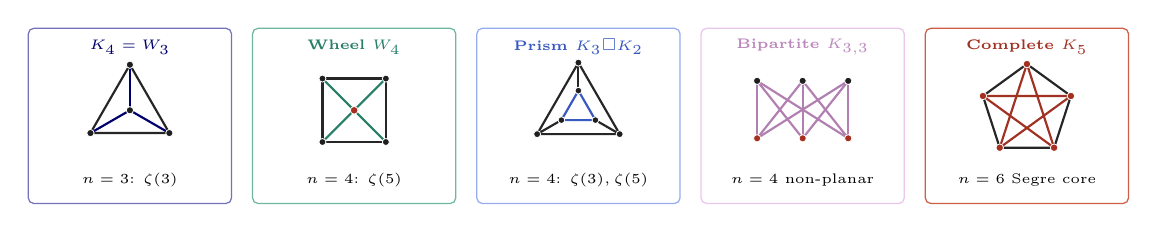
\begin{tikzpicture}[scale=0.89]
  % 1. K_4
  \begin{scope}[shift={(-6.40,0)}]
    \draw[rounded corners=2pt, draw=NavyBlue!55, fill=white, line width=0.45pt] (-1.45,-1.25) rectangle (1.45,1.25);
    \node[font=\tiny\bfseries, text=NavyBlue!85!black] at (0,0.98) {$K_4 = W_3$};
    \coordinate (k0) at (0,0.08);
    \foreach \idx/\ang in {1/90, 2/210, 3/330} \coordinate (k\idx) at ($(0,0.08)+({\ang}:0.65cm)$);
    \draw[prop] (k1)--(k2)--(k3)--cycle;
    \foreach \idx in {1,2,3} \draw[prop, NavyBlue!85!black] (k0)--(k\idx);
    \foreach \idx in {0,1,2,3} \filldraw[v0] (k\idx) circle (0.052cm);
    \node[font=\tiny] at (0,-0.92) {$n=3$: $\zeta(3)$};
  \end{scope}
  % 2. W_4
  \begin{scope}[shift={(-3.20,0)}]
    \draw[rounded corners=2pt, draw=PineGreen!55, fill=white, line width=0.45pt] (-1.45,-1.25) rectangle (1.45,1.25);
    \node[font=\tiny\bfseries, text=PineGreen!85!black] at (0,0.98) {Wheel $W_4$};
    \coordinate (w0) at (0,0.08);
    \foreach \idx/\ang in {1/45, 2/135, 3/225, 4/315} \coordinate (w\idx) at ($(0,0.08)+({\ang}:0.64cm)$);
    \draw[prop] (w1)--(w2)--(w3)--(w4)--cycle;
    \foreach \idx in {1,2,3,4} \draw[prop, PineGreen!85!black] (w0)--(w\idx);
    \filldraw[vbiv] (w0) circle (0.055cm);
    \foreach \idx in {1,2,3,4} \filldraw[v0] (w\idx) circle (0.05cm);
    \node[font=\tiny] at (0,-0.92) {$n=4$: $\zeta(5)$};
  \end{scope}
  % 3. Prism
  \begin{scope}[shift={(0,0)}]
    \draw[rounded corners=2pt, draw=RoyalBlue!55, fill=white, line width=0.45pt] (-1.45,-1.25) rectangle (1.45,1.25);
    \node[font=\tiny\bfseries, text=RoyalBlue!85!black] at (0,0.98) {Prism $K_3\square K_2$};
    \foreach \idx/\ang in {1/90, 2/210, 3/330} {
      \coordinate (po\idx) at ($(0,0.08)+({\ang}:0.68cm)$);
      \coordinate (pi\idx) at ($(0,0.08)+({\ang}:0.28cm)$);
    }
    \draw[prop] (po1)--(po2)--(po3)--cycle;
    \draw[prop, RoyalBlue!85!black] (pi1)--(pi2)--(pi3)--cycle;
    \foreach \idx in {1,2,3} { \draw[prop] (po\idx)--(pi\idx); \filldraw[v0] (po\idx) circle (0.05cm); \filldraw[v0] (pi\idx) circle (0.048cm); }
    \node[font=\tiny] at (0,-0.92) {$n=4$: $\zeta(3),\zeta(5)$};
  \end{scope}
  % 4. K_{3,3}
  \begin{scope}[shift={(3.20,0)}]
    \draw[rounded corners=2pt, draw=Plum!60, fill=white, line width=0.45pt] (-1.45,-1.25) rectangle (1.45,1.25);
    \node[font=\tiny\bfseries, text=Plum!85!black] at (0,0.98) {Bipartite $K_{3,3}$};
    \foreach \idx/\xx in {1/-0.65, 2/0.0, 3/0.65} { \coordinate (ka\idx) at (\xx,0.50); \coordinate (kb\idx) at (\xx,-0.32); }
    \foreach \p in {1,2,3} \foreach \q in {1,2,3} \draw[prop, Plum!80!black] (ka\p)--(kb\q);
    \foreach \idx in {1,2,3} { \filldraw[v0] (ka\idx) circle (0.052cm); \filldraw[vbiv] (kb\idx) circle (0.052cm); }
    \node[font=\tiny] at (0,-0.92) {$n=4$ non-planar};
  \end{scope}
  % 5. K_5
  \begin{scope}[shift={(6.40,0)}]
    \draw[rounded corners=2pt, draw=BrickRed!65, fill=white, line width=0.45pt] (-1.45,-1.25) rectangle (1.45,1.25);
    \node[font=\tiny\bfseries, text=BrickRed!85!black] at (0,0.98) {Complete $K_5$};
    \foreach \idx/\ang in {0/90, 1/18, 2/306, 3/234, 4/162} \coordinate (c\idx) at ($(0,0.08)+({\ang}:0.66cm)$);
    \draw[prop] (c0)--(c1)--(c2)--(c3)--(c4)--cycle;
    \draw[prop, BrickRed!85!black] (c0)--(c2)--(c4)--(c1)--(c3)--cycle;
    \foreach \idx in {0,1,2,3,4} \filldraw[vbiv] (c\idx) circle (0.054cm);
    \node[font=\tiny] at (0,-0.92) {$n=6$ Segre core};
  \end{scope}
\end{tikzpicture}
\caption{Canonical $3$-connected non-series--parallel Feynman cores named in Obstacle~2(b): $K_4 = W_3$ ($n=3$), $W_4$, the planar prism $K_3\square K_2$, the non-planar Kuratowski graph $K_{3,3}$ ($n=4$), and the $4$-regular non-planar complete graph $K_5$ ($n=6$).}
\label{fig:nonsp-core-gallery}
\end{figure}

\subsection{Closed Two-Loop Theta Kernels, \texorpdfstring{$T\ge 2$}{T>=2} Vanishing, and Ohm/Segre Locality}
\label{subsec:theta-t2-ohm}

\begin{theorem}[Closed two-loop $\theta(n_1,n_2,n_3)$ kernels across $(H,T)$ and all-loop companion families~{\cite{Repo9e833c8}}]
\label{thm:theta-closed}
For a tight two-loop theta graph $\theta(n_1,n_2,n_3)$ ($n_1+n_2+n_3 = 2D+1$, $1 \le n_P \le D$) with path resistances $R_P = \sum_{\substack{q\in\{1,\dots,n_P\}\\\mathrm{path\ edges}}}t_{P,q}$, interior source matrices $\Lambda_P \in \C^{H\times(n_P-1)}$, $2H\times 2H$ determinants $D_\theta(\lambda) := \det\bigl(\begin{smallmatrix}\Lambda_1 & \Lambda_2 & 0\\ 0 & \Lambda_2 & \Lambda_3\end{smallmatrix}\bigr)$ ($T=1$) and $Q(v) := \det\bigl(\begin{smallmatrix}v & 0 & \Lambda_1 & \Lambda_2 & 0\\ 0 & v & 0 & \Lambda_2 & \Lambda_3\end{smallmatrix}\bigr)$ ($T=0$), and mean source $\bar{L}_i := \lambda^{\mathrm{top}}_i + \sum_{\substack{P\in\{1,2,3\}\\\mathrm{paths}}}\sum_{\substack{m\in\{1,\dots,n_P-1\}\\\mathrm{interior\ verts}}}\frac{n_P-m}{n_P}\lambda^{P,m}_i$, in cycle basis $C_3$ ($K_{\mathrm{htk}} = (-1)^{(n_2+1)D}K[C_3]$):
\begin{equation}
\label{eq:theta-closed-both}
\begin{aligned}
K_{T=1}[C_3](\lambda;0) &= (-1)^{\frac{H(H+1)}{2}}\frac{D_\theta(\lambda)\prod_{P=1}^3\Gamma(H+\frac{3}{2}-n_P)}{2\,\Gamma(H+\frac{3}{2})\prod_{P=1}^3(n_P-1)!},\\
K_{T=0}[C_3](\lambda;0) &= (-1)^{\frac{H(H+1)}{2}+1}\frac{\prod_{P=1}^3(H-n_P)!\,Q(\bar{L})}{(H+1)!\prod_{P=1}^3(n_P-1)!}.
\end{aligned}
\end{equation}
Moreover, even-$n$ $(1,1)$ endpoint fans evaluate to $\frac{(4\pi)^{n/2}}{(n+1)(n!)^2}(\lambda_1\lambda_{n+1})^{n/2}$, $\C^3$ $n$-box ladders evaluate to $\frac{(-1)^{n-1}2^{n+1}\Delta^n}{(n+2)!(n!)^2((n+1)!)^2}$, and $(0,1)$ $N$-edge bananas ($n=N-1$) evaluate to $\pi^{n/2}$ ($n$ even, $0$ odd), assembling the Moyal weight $2^{-N}$.
\end{theorem}

\begin{proof}
At $T=1$, $\rho_2(M) = (R_1\dd R_2\wedge\dd R_3 - R_2\dd R_1\wedge\dd R_3 + R_3\dd R_1\wedge\dd R_2)/(2U_\theta^{3/2})$ annihilates $\dd\log(R_1/R_2)$ and $\dd\log(R_2/R_3)$, eliminating endpoint potential differentials and factoring the integral into $\prod_{P=1}^3\vol(\Delta^{n_P-1})$ times a Dirichlet half-integer beta integral in $w_P = R_P^{-1}/(R_1^{-1}+R_2^{-1}+R_3^{-1})$. At $T=0$, quadratic polarization of $Q(L(x))$ vanishes on collinear columns within a single $\Lambda_P$, so simplex expectation commutes with $Q$: $\mathbb{E}_x[Q(L(x))] = Q(\bar{L})$.
\end{proof}

\begin{example}[Pareto $\alpha_{\mathrm{Par}} = 6/5$ Monte Carlo trap and $5\mathrm{D}$ CS $\theta(1,3,3), \theta(2,2,3)$ evaluation]
\label{ex:pareto-and-5d-theta}
Near the codimension-$3$ corner $U_\theta \to \rho_{\mathrm{corner}}$ of $\Delta^4$ on $\theta(1,2,2)$ at $(H,T)=(1,1)$, $|D(t)| = |D_\theta|/(2U_\theta^{5/2})$ follows $\mathbb{P}(|D| > x) = 8(c/x)^{6/5} + \mathcal{O}(x^{-8/5})$ ($\alpha_{\mathrm{Par}} = \frac{6}{5} < 2$), giving $\mathbb{E}[D^2] = \infty$ under naive uniform simplex sampling!

Exact evaluation~\eqref{eq:theta-closed-both} at $(H,T) = (2,1)$ ($D=3$, $H+\frac{3}{2} = \frac{7}{2}$, $\Gamma(\frac{7}{2}) = \frac{15}{8}\sqrt{\pi}$) yields for external momenta $p^{(1)},\dots,p^{(4)}$:
\[
\begin{aligned}
K_{133} &= -\frac{\frac{3}{4}\pi^{3/2}}{2\cdot\frac{15}{8}\sqrt{\pi}\cdot 0!\,2!\,2!}[p^{(1)}p^{(2)}][p^{(3)}p^{(4)}] = -\frac{\pi}{20}[p^{(1)}p^{(2)}][p^{(3)}p^{(4)}],\\
K_{223} &= +\frac{\pi}{30}[p^{(1)}p^{(2)}][p^{(3)}p^{(4)}],
\end{aligned}
\]
where $(-1)^{(2+1)\cdot 3} = -1$ flips the sign on $\theta(2,2,3)$.
\end{example}

\begin{theorem}[Algebraic Pfaffian vanishing $\rho_n(M)\wedge\rho_n(M) = 0$ for $T \ge 2$ and Ohm/Segre locality~{\cite{Repo9e833c8}}]
\label{thm:ohm-locality}
\leavevmode
\begin{enumerate}[label=(\arabic*),leftmargin=*]
  \item \emph{All-loop bulk vanishing at $T \ge 2$:} For every smooth positive-definite symmetric $n\times n$ matrix family $M_{rs}(t)$ ($n \ge 1$), $\rho_n(M)\wedge\rho_n(M) = 0$; hence at $T \ge 2$ and zero topological momentum ($\kappa = 0$), $\Omega_\Gamma = 0$ and $K_\Gamma(\lambda;z) = 0$ identically for all $n \ge 1$ ($4\mathrm{D}$ CS on $\RR^2\times\C$, $3\mathrm{D}$ CS on $\RR^3$).

  \item \emph{Differential-form Ohm locality, $T=1$ contact, $k=2$ closing edge, and $k\ge 4$ Segre quadrics:} Partitioning $\Gamma = S \cup O$ along $k = |\partial S|$ boundary terminals with interior $S^\circ$, Schur complement $L_{\mathrm{red}} := L_{\partial\partial} - L_{\partial\circ}L_{\circ\circ}^{-1}L_{\circ\partial}$, impedance $Z := L_{\mathrm{red}}^+$, and harmonic transfer $h^a{}_u := -(L_{\circ\circ}^{-1})^{uw}(L_{\circ\partial})_{wa}$ ($p_{\mathrm{out}} : t_S \mapsto (Z,h)$) factors $\Omega_\Gamma = \eps\,\Omega_S\wedge(\Omega_{\mathrm{out}}\circ p_{\mathrm{out}})$ ($\eps \in \{\pm 1\}$).

  At $T = 1$, conditioning $\tau_\circ$ leaves an internal fluctuation source $\xi_u$ with covariance $\langle\xi_u\xi_v\rangle = \frac{1}{2}(L_{\circ\circ})_{uv}$ (Figure~\ref{fig:ohm-segre}(a)). At $k=2$, closing $S$ by $e_*$ into $\widehat{S} := S\cup\{e_*\}$ satisfies $\int P_{\mathrm{num}}U_S^{-p_1}U_{S/pq}^{-p_2}\iota_E\mathrm{dvol}_S = \frac{\Gamma(p_1+p_2)}{\Gamma(p_1)\Gamma(p_2)}I_{p_1+p_2}(\widehat{S}; \alpha_S, \alpha_{e_*}=p_1)$. At valence $k \ge 4$, star elimination produces rank-$1$ conductances $c_{pq} = g_p g_q / G_{\mathrm{tot}}$ cut out by the codimension-$\frac{1}{2}k(k-3)$ \textbf{Segre determinantal quadrics} $c_{pq}c_{lm} = c_{pl}c_{qm} = c_{pm}c_{ql}$ (codimension $2$ at $k=4$ on $K_5 \to K_4$, Figure~\ref{fig:ohm-segre}(b)).
\end{enumerate}
\end{theorem}

\begin{proof}
In~(1), set $X^r{}_s := (M^{-1})^{rp}\dd M_{ps}$. Since $A_{rs} = -\frac{1}{2}\dd M_{rp}(M^{-1})^{pq}\dd M_{qs}$ has entries in the commutative ring $\Omega^{\mathrm{even}}$, $\Pf(A)^2 = \det(A)$ gives $\rho_n(M)\wedge\rho_n(M) = (-\frac{1}{2})^n\det(X\wedge X)$. Cyclically shifting the last odd $1$-form $X^{r_{2j}}{}_{r_1}$ across $2j-1$ odd $1$-forms gives $\tr((X\wedge X)^j) = -\tr((X\wedge X)^j) = 0$ ($\forall\,j\ge 1$), so Newton's identities force $\det(X\wedge X) = 0$. In~(2), splitting internal currents into harmonic terminal flows and Dirichlet flows block-diagonalizes $M_\Gamma = \diag(M_S, M_O + D_{\mathrm{inc}}\text{-block})$; completing the Gaussian square on $\tau_\circ$ gives $\langle\xi_u\xi_v\rangle = \frac{1}{2}(L_{\circ\circ})_{uv}$; beta integration on $t_{e_*}$ proves the $k=2$ identity; and rank-$1$ $2\times 2$ minors of $(g_p g_q)$ cut out the Segre variety.
\end{proof}

\begin{figure}[H]
\centering
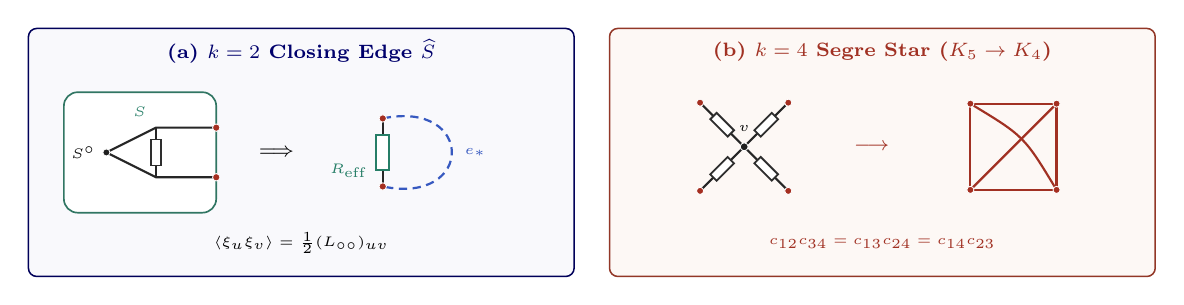
\begin{tikzpicture}[scale=0.90]
  % Left: k=2 Ohm factorization & closing edge
  \begin{scope}[shift={(-4.10,0)}]
    \draw[rounded corners=3pt, draw=NavyBlue!70!black, fill=NavyBlue!2.5, line width=0.55pt] (-3.85,-1.75) rectangle (3.85,1.75);
    \node[font=\scriptsize\bfseries, text=NavyBlue!85!black] at (0,1.42) {(a) $k=2$ Closing Edge $\widehat{S}$};
    \draw[rounded corners=5pt, draw=PineGreen!75!black, fill=white, line width=0.6pt] (-3.35,-0.85) rectangle (-1.20,0.85);
    \node[font=\tiny\bfseries, text=PineGreen!85!black] at (-2.28,0.58) {$S$};
    \coordinate (tp) at (-1.20, 0.35); \coordinate (tq) at (-1.20,-0.35);
    \draw[prop] (-2.75,0) -- (-2.05,0.35) -- (tp);
    \draw[prop] (-2.75,0) -- (-2.05,-0.35) -- (tq);
    \draw[prop] (-2.05,0.35) -- node[iecres, rotate=90, scale=0.55] {} (-2.05,-0.35);
    \filldraw[v0] (-2.75,0) circle (0.05cm) node[left=1pt, font=\tiny] {$S^\circ$};
    \filldraw[vbiv] (tp) circle (0.052cm); \filldraw[vbiv] (tq) circle (0.052cm);
    \node[font=\scriptsize] at (-0.35,0) {$\Longrightarrow$};
    \coordinate (ep) at (1.15, 0.48); \coordinate (eq) at (1.15,-0.48);
    \draw[prop] (ep) -- node[iecres, rotate=90, scale=0.75, draw=PineGreen!85!black] (Reff) {} (eq);
    \node[left=2pt, font=\tiny, text=PineGreen!85!black] at (Reff.west) {$R_{\mathrm{eff}}$};
    \draw[line width=0.8pt, densely dashed, draw=RoyalBlue!85!black] (ep) .. controls (2.45,0.75) and (2.45,-0.75) .. node[right=1pt, font=\tiny, text=RoyalBlue!85!black] {$e_*$} (eq);
    \filldraw[vbiv] (ep) circle (0.052cm); \filldraw[vbiv] (eq) circle (0.052cm);
    \node[font=\tiny] at (0,-1.28) {$\langle\xi_u\xi_v\rangle = \frac{1}{2}(L_{\circ\circ})_{uv}$};
  \end{scope}

  % Right: k=4 Segre star elimination
  \begin{scope}[shift={(4.10,0)}]
    \draw[rounded corners=3pt, draw=BrickRed!75!black, fill=BrickRed!2.5, line width=0.55pt] (-3.85,-1.75) rectangle (3.85,1.75);
    \node[font=\scriptsize\bfseries, text=BrickRed!85!black] at (0,1.42) {(b) $k=4$ Segre Star ($K_5\to K_4$)};
    \begin{scope}[shift={(-1.95,0.08)}]
      \coordinate (sv) at (0,0);
      \foreach \idx/\ang in {1/45, 2/135, 3/225, 4/315} {
        \coordinate (u\idx) at (\ang:0.88cm);
        \draw[prop] (sv) -- node[iecres, sloped, scale=0.52] {} (u\idx);
        \filldraw[vbiv] (u\idx) circle (0.05cm);
      }
      \filldraw[v0] (sv) circle (0.056cm) node[above=2pt, font=\tiny] {$v$};
    \end{scope}
    \node[font=\scriptsize, text=BrickRed!85!black] at (-0.15,0.08) {$\longrightarrow$};
    \begin{scope}[shift={(1.85,0.08)}]
      \foreach \idx/\ang in {1/45, 2/135, 3/225, 4/315} \coordinate (w\idx) at (\ang:0.86cm);
      \draw[prop, BrickRed!85!black] (w1)--(w2)--(w3)--(w4)--cycle;
      \draw[prop, BrickRed!85!black] (w1)--(w3);
      \draw[prop, BrickRed!85!black] (w2) .. controls (0.15,0.15) .. (w4);
      \foreach \idx in {1,2,3,4} \filldraw[vbiv] (w\idx) circle (0.05cm);
    \end{scope}
    \node[font=\tiny, text=BrickRed!85!black] at (0,-1.28) {$c_{12}c_{34} = c_{13}c_{24} = c_{14}c_{23}$};
  \end{scope}
\end{tikzpicture}
\caption{Ohm locality vs.\ Segre obstruction in Theorem~\ref{thm:ohm-locality}(2): (a)~two-terminal Schur reduction onto $R_{\mathrm{eff}} = U_{S/pq}/U_S$ with closing edge $e_*$ and $T=1$ Dirichlet covariance $\frac{1}{2}(L_{\circ\circ})_{uv}$; (b)~four-terminal star elimination inside $K_5$ restricting $c_{pq} = g_p g_q/G_{\mathrm{tot}}$ to the codimension-$2$ Segre quadric locus.}
\label{fig:ohm-segre}
\end{figure}

\subsection{Fixed-Core Algebraic de~Rham Stabilization and Sharp \texorpdfstring{$n$}{n}-Spoke Wheel Span}
\label{subsec:stabilization-wheels}

For a fixed connected core graph $G = (V,E)$ ($N = |E| \ge 2$, loop number $h_G = N-|V|+1$), define the integer-pole period space $\mathcal{P}_q(G) := \Span_{\QQ}\{I_q(G;\alpha) : \alpha_e \in \ZZ_{>0},\ \sum_{\substack{e\in E\\\mathrm{edges}}}\alpha_e = q h_G,\ \sum_{\substack{e\in S\\\mathrm{subset}}}\alpha_e > q\,h(S)\ \forall\,\varnothing\neq S\subsetneq E\}$, where $I_q(G;\alpha) := \int_{\mathbb{RP}^{N-1}_{>0}}(\prod_{\substack{e\in E\\\mathrm{edges}}}t_e^{\alpha_e-1})U_G(t)^{-q}\Omega_G$ carries unnormalized Schwinger weights without $\Gamma(\alpha_e)$ factors.

\begin{theorem}[Fixed-core relative algebraic de~Rham finiteness and pole stabilization~{\cite{Panzer15,Repo9e833c8}}]
\label{thm:core-stabilization}
For every connected core graph $G = (V,E)$ ($m := |E|-1$):
\begin{enumerate}[label=(\arabic*),leftmargin=*]
  \item On each Hepp sector $0 < t_{\sigma(1)} < \dots < t_{\sigma(N)} = 1$ ($t_{\sigma(p)} = \prod_{\substack{j\in\{p,\dots,m\}\\\mathrm{sector\ vars}}}x_j$), Kruskal's greedy spanning tree factors $U_G(t(x)) = (\prod_{\substack{j\in\{1,\dots,m\}\\\mathrm{prefixes}}}x_j^{h(S_j)})U_\sigma(x)$ with $U_\sigma \in 1 + \ZZ_{\ge 0}[x_1,\dots,x_m]$ and $1 \le U_\sigma(x) \le \tau_G$ on $[0,1]^m$. Signed $\omega_{P,q} = P(t)U_G(t)^{-q}\Omega_G$ converges absolutely precisely when every collected monomial of $P$ obeys $\sum_{\substack{e\in S\\\mathrm{subset}}}\alpha_e > q\,h(S)$ ($\forall\,\varnothing\neq S\subsetneq E$).

  \item Every convergent $\omega_{P,q}$ pulls back into the finite-dimensional relative algebraic de~Rham quotient ($A_\sigma := \QQ[x_1,\dots,x_m, U_\sigma^{-1}]$, $X_\sigma := \mathbb{A}^m_{\QQ}\setminus\{U_\sigma=0\}$, $B_\sigma := \bigcup_{\substack{p\in\{1,\dots,m\}\\\mathrm{faces}}}\{x_p(1-x_p)=0\}$):
  \begin{equation}
  \label{eq:rel-dr-quotient}
  H^m_{\mathrm{dR}}(X_\sigma, B_\sigma; \QQ) = \frac{A_\sigma}{\sum_{\substack{p\in\{1,\dots,m\}\\\mathrm{cube\ coords}}}\partial_{x_p}\bigl(x_p(1-x_p)A_\sigma\bigr)},\qquad
  \dim_{\QQ}\bigcup_{r\ge 1}\mathcal{P}_r(G) < \infty,
  \end{equation}
  and cotree pole-raising $I_q(G;\alpha) = \sum_{\substack{T\subset G\\\mathrm{spanning\ trees}}}I_{q+1}(G;\alpha + \mathbf{1}_{E\setminus T})$ proves $\mathcal{P}_q(G) \subseteq \mathcal{P}_{q+1}(G)$ and $\mathcal{P}_q(G) = \bigcup_{r\ge 1}\mathcal{P}_r(G)$ for all sufficiently large $q$.
\end{enumerate}
\end{theorem}

\begin{proof}
In~(1), every spanning tree $T$ satisfies $|(E\setminus T)\cap S_j| \ge h(S_j)$ with simultaneous equality attained by Kruskal's greedy tree~\cite{Panzer15}; distinct homogeneous $t$-monomials map to distinct $x$-monomials, preventing cancellation of any $x_p^{r}$ ($r \le -1$) divergence on $\{x_p=0\}\cap(0,1)^{m-1}$. In~(2), the affine log complex $\Omega^\bullet_{X_\sigma}(\log B_\sigma)(-B_\sigma)$ computes $H^m_{\mathrm{dR}}(X_\sigma,B_\sigma;\QQ)$ as~\eqref{eq:rel-dr-quotient}, which is finite-dimensional by Grothendieck's algebraic de~Rham theorem; multiplying the integrand by $U_G(t)/U_G(t) = \sum_{\substack{T\\\mathrm{trees}}}(\prod_{\substack{e\notin T\\\mathrm{cotree}}}t_e)/U_G(t)$ preserves $\sum_{\substack{e\in S\\\mathrm{subset}}}(\alpha_e + \mathbf{1}_{e\notin T}) \ge \sum_{\substack{e\in S\\\mathrm{subset}}}\alpha_e + h(S) > (q+1)h(S)$, embedding $\mathcal{P}_q(G) \subseteq \mathcal{P}_{q+1}(G)$ inside a finite-dimensional $\QQ$-space.
\end{proof}

\begin{theorem}[Complete $n$-spoke wheel scalar period span without $\QQ$-independence assumptions~{\cite{Repo9e833c8}}]
\label{thm:wheel-span}
For every $n$-spoke wheel $W_n$ ($n \ge 3$) and every integer $q \ge \max(3, n-1)$,
\begin{equation}
\label{eq:wheel-exact-span}
\mathcal{P}_q(W_n) = \QQ + \sum_{\substack{j\in\{2,\dots,n-1\}\\\mathrm{odd\ zetas}}}\QQ\,\zeta(2j-1).
\end{equation}
\end{theorem}

\begin{proof}\leavevmode
\begin{proofpart}{Step 1: Upper inclusion via bilateral Laplace oddness}
Expanding $I_q(W_n;\alpha)$ in $\RR^{2q}$ spherical harmonics of degree $\nu \ge 0$ ($s = \nu+q-1$) produces $\sum_{\substack{s\ge q-1\\\mathrm{modes}}}M_q(s)F(s)$, where $M_q(-s) = M_q(s)$ has a double zero at $s=0$ and bilateral Laplace convolution makes $F(-s) = -F(s)$ odd of pole order $\le 2n-1$. Opposite shifted poles $\pm h$ cancel all even zeta values, leaving rational harmonic sums plus $\zeta(3),\zeta(5),\dots,\zeta(2n-3)$.
\end{proofpart}
\begin{proofpart}{Step 2: Triangular odd-zeta basis and all-$q$ factorial positivity on $K_4 = W_3$}
Radial wheels ($a_p = q'-1, \rho_p = 1$, $2 \le q' \le n-1$) have lowest zeta $\zeta(2n-2q'+1)$ with nonzero coefficient $2\binom{2n-2}{n-1}/(2q'-2)!$, triangulating $\zeta(3),\dots,\zeta(2n-3) \in \mathcal{P}_{n-1}(W_n)$ after multiplying by $U_{W_n}^{n-1-q'}$. On $K_4$ at path-complementary weights $(q-1,1,1;1,q-1,q-1)$, pairing shifts gives $I_q = R_q + \frac{12((q-2)!)^2}{(2q-2)!}\zeta(3)$ ($R_3 = -\frac{1}{6}$, $R_4 = \frac{7}{360}$, $R_q > 0$ checked for $4 \le q \le 20$). On $\Delta^5$, $U_{K_4}(t) \le \binom{6}{3}(\frac{1}{6})^3 = \frac{5}{54}$, giving $I_q \ge (\frac{54}{5})^q\frac{((q-2)!)^3}{(3q-1)!}$. Dividing by the $\zeta(3)$ coefficient defines $L_q := (\frac{54}{5})^q\frac{(q-2)!(2q-2)!}{12(3q-1)!}$, which obeys $\frac{L_{q+1}}{L_q} = \frac{36(q-1)(2q-1)}{5(3q+1)(3q+2)} > 1$ for $q \ge 6$ and $L_{21} > \frac{5}{4} > \zeta(3)$, proving $R_q > 0$ for all $q \ge 21$! Star--triangle and parallel merges embed $K_4$ into $W_n$ at $q=n-1$ with prefactor $1/((q-2)!)^3$, placing $1 \in \mathcal{P}_{n-1}(W_n)$ and proving~\eqref{eq:wheel-exact-span}.
\end{proofpart}
\end{proof}

\begin{lemma}[{Two-terminal closing-edge beta identity and $K_4$ simplex bound $U_{K_4} \le \frac{2}{27}$}]
\label{lem:closing-edge-k4}
\leavevmode
\begin{enumerate}[label=(\arabic*),leftmargin=*]
  \item Let $S$ be a $2$-terminal resistor network with terminals $\{p,q\}$, Kirchhoff polynomials $U_S(t)$ and $U_{S/pq}(t) = R_{\mathrm{eff}}(t)U_S(t)$, and closing edge $e_* = \{p,q\}$ forming $\widehat{S} := S\cup\{e_*\}$ ($U_{\widehat{S}}(t,t_{e_*}) = t_{e_*}U_S(t) + U_{S/pq}(t)$). For every monomial $P_{\mathrm{num}}(t) = \prod_{\substack{e\in S\\\mathrm{edges}}}t_e^{\alpha_e-1}$ and $p_1,p_2 > 0$ with $\sum_{\substack{e\in S\\\mathrm{edges}}}\alpha_e = (p_1+p_2)h_S + p_2$,
  \[
  \int_{\mathbb{RP}^{|S|-1}_{>0}}\frac{P_{\mathrm{num}}(t)}{U_S(t)^{p_1}U_{S/pq}(t)^{p_2}}\,\iota_E\mathrm{dvol}_S = \frac{\Gamma(p_1+p_2)}{\Gamma(p_1)\Gamma(p_2)}\,I_{p_1+p_2}(\widehat{S};\, \alpha_S, \alpha_{e_*} = p_1).
  \]

  \item On $K_4$ ($16$ spanning trees out of $\binom{6}{3} = 20$ edge triples), $U_{K_4}(t) \le \frac{2}{27} < \frac{5}{54}$ across $\Delta^5$, $\frac{L_7}{L_6} = \frac{99}{95} > 1$, and $R_q \neq 0$ implies $1 \in \mathcal{P}_q(K_4)$ purely algebraically without invoking $\QQ$-irrationality of $\zeta(3)$.
\end{enumerate}
\end{lemma}

\begin{proof}\leavevmode
\begin{proofpart}{Claim 1: Closing-edge Euler beta integral}
Deprojectivize $\widehat{S}$ by fixing $t_{e_0} = 1$ inside $S$ and integrating $t_{e_*} \in (0,\infty)$ via $t_{e_*} = u\,U_{S/pq}(t)/U_S(t)$:
\[
\int_0^\infty\frac{t_{e_*}^{p_1-1}\,\dd t_{e_*}}{\bigl(t_{e_*}U_S(t) + U_{S/pq}(t)\bigr)^{p_1+p_2}} = \frac{\Gamma(p_1)\Gamma(p_2)}{\Gamma(p_1+p_2)}\,U_S(t)^{-p_1}U_{S/pq}(t)^{-p_2},
\]
which integrates over $\mathbb{RP}^{|S|-1}_{>0}$ to the stated identity.
\end{proofpart}
\begin{proofpart}{Claim 2: Simplex maximum and rational isolation of $R_q$}
On $\Delta^5$ ($\sum_{\substack{e\in E(K_4)\\\mathrm{edges}}}t_e = 1$), Maclaurin's inequality gives $e_3(t) \le \binom{6}{3}(\frac{1}{6})^3 = \frac{5}{54}$, and subtracting the $4$ triangle cycles at the log-concave symmetric maximum $t_e = \frac{1}{6}$ attains $U_{K_4}(\frac{1}{6},\dots,\frac{1}{6}) = 16\cdot 6^{-3} = \frac{2}{27} < \frac{5}{54}$, while $\frac{L_7}{L_6} = \frac{36\cdot 5\cdot 11}{5\cdot 19\cdot 20} = \frac{99}{95} > 1$. Since $I_3(K_4;1^6) = 6\zeta(3)$ lifts into $\mathcal{P}_q(K_4)$ via $U_{K_4}^{q-3}$, subtracting $\frac{2((q-2)!)^2}{(2q-2)!}$ times that lifted vector from $I_q(K_4;q-1,1,1,1,q-1,q-1) = R_q + \frac{12((q-2)!)^2}{(2q-2)!}\zeta(3)$ isolates $R_q \in \mathcal{P}_q(K_4)\cap\QQ^\times$, proving $1 \in \mathcal{P}_q(K_4)$ unconditionally.
\end{proofpart}
\end{proof}

\subsection{Non-Planar \texorpdfstring{$K_5$}{K\_5} Through \texorpdfstring{$q=9$}{q=9} and All Three Six-Loop \texorpdfstring{$\C^2$}{C\^2} Kernels}
\label{subsec:k5-periods-sixloop}

On $\C^2$ at four loops ($13$ graphs, $2{,}359$ bracket coefficients), sliding Ward identities on the $60$ seven-vertex graphs have exact rational rank $2{,}344/2{,}359$ (concentrating all $15$ null vectors on $W_4$, restricting to $0$ on all $23$ four-loop product forests!), and $5$ Graph-$9$ laws $+ 8$ wheel IBPs $+ 2$ Gegenbauer masters $20\zeta(5)$ and $\frac{5}{3}(\zeta(3)-\zeta(5))$ close all $3{,}892$ triples in $\QQ+\QQ\zeta(3)+\QQ\zeta(5)$ (while the $5$-loop zigzag $Z_5$ carries $P(Z_5) = \frac{441}{8}\zeta(7)$~\cite{Schnetz10}).

\begin{theorem}[Non-planar $K_5$ closure through $q=8$, tower-input derivation, and $73$ guarded $q=9$ orbits~{\cite{CSS13,Repo9e833c8}}]
\label{thm:k5-periods}
Complete $K_5$ ($|V|=5,|E|=10$) at $\infty$ to $K_6$ ($\beta_e = q - \alpha_e$, $J_q(\beta) := \Gamma(q)I_q(K_5;q-\beta)/\prod_{\substack{e\subset K_5\\\mathrm{edges}}}\Gamma(\beta_e)$).
\begin{enumerate}[label=(\arabic*),leftmargin=*]
  \item Because $10$ propagators on $4$ integration vertices in $\RR^{2q}$ match $\binom{5}{2} = 10$ scalar products, vertex IBP $(\mathrm{X})$ plus dimension shift $(\mathrm{DS})$ solves \textbf{all $54{,}391$ convergent $K_5$ orbits for $q \le 8$} ($1.07\times 10^7$ rows) in $\QQ + \QQ\zeta(3) + \QQ\zeta(5)$ (e.g.\ $I_5(K_5;3^{10}) = -\frac{13}{15120} + \frac{19}{720}\zeta(3) - \frac{5}{168}\zeta(5)$), with zero $\zeta(7)$ or $\zeta(3)^2$.

  \item Combining $11$ $(\mathrm{X})$ rows $+ 1$ $(\mathrm{DS})$ row ($J_2 - 24J_3^{(9)} - 20J_3^{(14)} = 0$) with the cross-dimension radial-wheel relation $12I_3(W_4;\mathrm{rad}) + I_2(W_4;\mathrm{rad}) = \frac{10}{3}I_2(W_3;\mathrm{rad})$ ($J_2 + 6J_3^{(9)} = 20J_3^{(6)} + \frac{20}{3}J_3^{(5)}$) and telescoping $I_3(K_4;2,1,1;1,2,2) = \frac{1}{2}\zeta(3)-\frac{1}{6}$ proves the tower-input identity $J_2 = 4J_3^{(14)} + 16J_3^{(6)} + \frac{16}{3}J_3^{(5)}$ analytically.

  \item Wishart transverse Gram integration yields the $130$-term Cayley--Menger downward identity $J_q(\beta) = -\frac{1}{4(q-2)(2q-3)(2q-5)}\sum_{\substack{m\\\mathrm{cycle\ covers}}}c_m J_{q-1}(\beta-m)$, which converges termwise precisely when $\beta_e \le q-2$ ($\forall\,e\subset K_6$) and $\sum_{\substack{e\subset S\\\mathrm{triangles}}}\beta_e \le 2q-3$ ($\forall\,|S|=3$), evaluating \textbf{all $73$ guarded $q=9$ $K_5$ orbits} ($4{,}905$ vectors: $13$ generic, $7\ T_1$, $53\ T_2$; e.g.\ $I_9(K_5;3,5,6,6,5,6,6,6,6,5) = \frac{1637270809}{3295339407360000} + \frac{50430067}{22884301440000}\zeta(3) - \frac{551}{181621440}\zeta(5)$).
\end{enumerate}
\end{theorem}

\begin{proof}
In~(1), Gaussian row elimination on $(\mathrm{X})+(\mathrm{DS})$ expresses interior $K_5$ weights via boundary $K_5-e \leftrightarrow \mathrm{prism}$ orbits closed in $\QQ+\QQ\zeta(3)+\QQ\zeta(5)$. In~(2), $M_{q+1}(s) = \frac{s^2-(q-1)^2}{2q(2q-1)}M_q(s)$ gives the radial-wheel recurrence, and eliminating $J_3^{(9)} = 2I_3(W_4;\mathrm{rad})$ between $J_2 = 24J_3^{(9)} + 20J_3^{(14)}$ and $J_2 + 6J_3^{(9)} = 20J_3^{(6)} + \frac{20}{3}J_3^{(5)}$ yields the $J_2$ relation. In~(3), comparing Wishart Jacobians at $m=2q-1$ vs.\ $2q-3$ inserts $\det S = -\frac{1}{16}\det_{\mathrm{CM}}$~\cite{CSS13}; Hamiltonian $6$-cycles prove necessity and sufficiency of the strict-cut guard, satisfied on all $73\times 130 = 9{,}490$ $q=9\to 8$ terms.
\end{proof}

Both hypotheses of the strict-cut guard in Theorem~\ref{thm:k5-periods}(3) are sharp and unavoidable when splitting the Gram integrand into separate lower-$q$ periods. At $q = 5$, the convergent weight $\alpha = (2,2,3,4,2,3,3,4,3,4)$ spawns a formal $q = 4$ term $\alpha' = (1,1,3,3,1,3,3,3,3,3)$ with positive edge weights whose triangle $012$ sum $1+1+1 = 3$ falls below the strict threshold $4 = 4\cdot 1$ (carrying Cayley--Menger coefficient $\frac{1}{8}$ and falling factorial $1$), diverging at $\{t_{01}=t_{02}=t_{12}=0\}$; similarly, at $q = 3$, naively dropping zero falling-factorial terms loses a finite boundary period!

\begin{theorem}[Reciprocal conductance reduction ($35\to 15$) and all three six-loop $\C^2$ $K_5$ kernels~{\cite{Repo9e833c8}}]
\label{thm:sixloop-k5}
At $(H,n) = (2,6)$ ($|V|=8, |I|=13$), $2$-Laman admissibility selects $30+10+60 = 100$ labelled $K_5$ subdivisions across three isomorphism classes (Figure~\ref{fig:sixloop-k5}). Contracting series chains and inverting $R_c = 1/g_c$ to $Q(g) := (\prod_{\substack{c\in\{1,\dots,10\}\\\mathrm{chains}}}g_c^5)\overline{P}(1/g)$ drops degree from $35$ to $15$ ($1.79\times 10^9 \to 683{,}834$ graphic-flat points/prime; $7$ primes $= 217$ bits $>$ Mahler bound $197$ bits), evaluating all three bare kernels at conserved benchmark sources:
\begin{equation}
\label{eq:sixloop-k5-values}
\begin{aligned}
K_{\mathrm{path+edge}} &= \frac{823413972469}{182891520000} - \frac{10923017647}{635040000}\zeta(3) + \frac{37445089}{2352000}\zeta(5) > 0,\\
K_{\mathrm{triangle}} &= \frac{362193894187}{18289152000} + \frac{1985715463}{42336000}\zeta(3) - \frac{12884579}{176400}\zeta(5) > 0,\\
K_{3\text{-}\mathrm{path}} &= -\frac{482542848959}{15240960000} - \frac{210499252657}{3810240000}\zeta(3) + \frac{20153461}{201600}\zeta(5) > 0.
\end{aligned}
\end{equation}
\end{theorem}

\begin{proof}
Each chain $c$ obeys $\deg_{R_c}\overline{P} \le n\,\rk C_{\{c\}} - 1 = 5$, so $Q(g)$ is a polynomial; nodal $K_5$ potentials have $\deg_g \le v-2 = 3$, bounding $\deg_g Q \le (n-1)(v-2) = 15$, reconstructed modulo $7$ primes and mapped into Theorem~\ref{thm:k5-periods}(1).
\end{proof}

\begin{figure}[H]
\centering
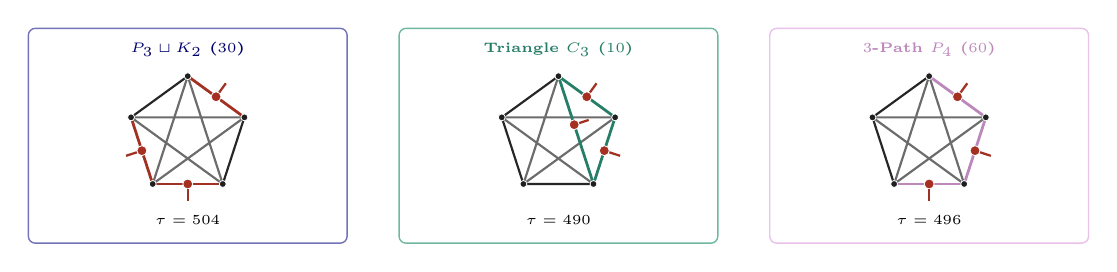
\begin{tikzpicture}[scale=0.88]
  % Shape 1
  \begin{scope}[xshift=-5.35cm]
    \draw[rounded corners=2.5pt, draw=NavyBlue!55, fill=white, line width=0.5pt] (-2.30,-1.55) rectangle (2.30,1.55);
    \node[font=\tiny\bfseries, text=NavyBlue!85!black] at (0,1.25) {$P_3\sqcup K_2$ ($30$)};
    \foreach \v/\ang in {0/90, 1/18, 2/306, 3/234, 4/162} \coordinate (p\v) at ({\ang}:0.86cm);
    \draw[line width=1.0pt, draw=BrickRed!85!black] (p0) -- node[vbiv, scale=0.82] (s5) {} (p1);
    \draw[prop] (p1)--(p2);
    \draw[line width=1.0pt, draw=BrickRed!85!black] (p2) -- node[vbiv, scale=0.82] (s6) {} (p3);
    \draw[line width=1.0pt, draw=BrickRed!85!black] (p3) -- node[vbiv, scale=0.82] (s7) {} (p4);
    \draw[prop] (p4)--(p0);
    \draw[prop, gray!85!black] (p0)--(p2)--(p4)--(p1)--(p3)--cycle;
    \draw[extleg] (s5)--++(54:0.24cm); \draw[extleg] (s6)--++(270:0.24cm); \draw[extleg] (s7)--++(198:0.24cm);
    \foreach \v in {0,1,2,3,4} \filldraw[v0] (p\v) circle (0.05cm);
    \node[font=\tiny] at (0,-1.22) {$\tau = 504$};
  \end{scope}
  % Shape 2
  \begin{scope}[xshift=0cm]
    \draw[rounded corners=2.5pt, draw=PineGreen!55, fill=white, line width=0.5pt] (-2.30,-1.55) rectangle (2.30,1.55);
    \node[font=\tiny\bfseries, text=PineGreen!85!black] at (0,1.25) {Triangle $C_3$ ($10$)};
    \foreach \v/\ang in {0/90, 1/18, 2/306, 3/234, 4/162} \coordinate (q\v) at ({\ang}:0.86cm);
    \draw[prop, gray!85!black] (q2)--(q4)--(q1)--(q3)--(q0);
    \draw[prop] (q2)--(q3)--(q4)--(q0);
    \draw[line width=1.0pt, draw=PineGreen!85!black] (q0) -- node[vbiv, scale=0.82] (t5) {} (q1);
    \draw[line width=1.0pt, draw=PineGreen!85!black] (q1) -- node[vbiv, scale=0.82] (t7) {} (q2);
    \draw[line width=1.0pt, draw=PineGreen!85!black] (q0) -- node[pos=0.45, vbiv, scale=0.82] (t6) {} (q2);
    \draw[extleg] (t5)--++(54:0.24cm); \draw[extleg] (t7)--++(342:0.24cm); \draw[extleg] (t6)--++(18:0.22cm);
    \foreach \v in {0,1,2,3,4} \filldraw[v0] (q\v) circle (0.05cm);
    \node[font=\tiny] at (0,-1.22) {$\tau = 490$};
  \end{scope}
  % Shape 3
  \begin{scope}[xshift=5.35cm]
    \draw[rounded corners=2.5pt, draw=Plum!65, fill=white, line width=0.5pt] (-2.30,-1.55) rectangle (2.30,1.55);
    \node[font=\tiny\bfseries, text=Plum!85!black] at (0,1.25) {$3$-Path $P_4$ ($60$)};
    \foreach \v/\ang in {0/90, 1/18, 2/306, 3/234, 4/162} \coordinate (r\v) at ({\ang}:0.86cm);
    \draw[prop, gray!85!black] (r0)--(r2)--(r4)--(r1)--(r3)--cycle;
    \draw[prop] (r3)--(r4)--(r0);
    \draw[line width=1.0pt, draw=Plum!85!black] (r0) -- node[vbiv, scale=0.82] (u5) {} (r1);
    \draw[line width=1.0pt, draw=Plum!85!black] (r1) -- node[vbiv, scale=0.82] (u6) {} (r2);
    \draw[line width=1.0pt, draw=Plum!85!black] (r2) -- node[vbiv, scale=0.82] (u7) {} (r3);
    \draw[extleg] (u5)--++(54:0.24cm); \draw[extleg] (u6)--++(342:0.24cm); \draw[extleg] (u7)--++(270:0.24cm);
    \foreach \v in {0,1,2,3,4} \filldraw[v0] (r\v) circle (0.05cm);
    \node[font=\tiny] at (0,-1.22) {$\tau = 496$};
  \end{scope}
\end{tikzpicture}
\caption{All three $2$-Laman admissible six-loop $K_5$ subdivision Feynman topologies on $\C^2$ ($|V|=8, |I|=13$, red dots $=$ bivalent external source vertices) evaluated in Theorem~\ref{thm:sixloop-k5}.}
\label{fig:sixloop-k5}
\end{figure}

\subsection{Complete \texorpdfstring{$T=1$}{T=1} Four-Loop Prism/\texorpdfstring{$K_{3,3}$}{K\_\{3,3\}}, \texorpdfstring{$3$}{3}-Terminal Locality, and \texorpdfstring{$5$}{5}-Loop \texorpdfstring{$\C^3$}{C\^3} \texorpdfstring{$\zeta(3)^2$}{zeta(3)\^2}}
\label{subsec:t1-and-bulk3}

\begin{theorem}[$5{,}054$ half-integer periods, $K_{K_{3,3}}\equiv 0$ parity vs.\ nonzero currents, and $3$-terminal $T=1$ locality~{\cite{Repo9e833c8}}]
\label{thm:t1-completion}
At $(H,T) = (1,1)$ and $n=4$ loops ($|V|=6, |I|=9$, $1{,}204$ bare + first-current monomials in $\QQ\pi^2\oplus\QQ\pi^4$):
\begin{enumerate}[label=(\arabic*),leftmargin=*]
  \item Closing $55{,}074$ regulator-free IBP rows uniquely determines \textbf{all $5{,}054$ convergent half-integer scalar periods} on $K_{3,3}$ ($q \in \{\frac{7}{2},\frac{9}{2},\frac{11}{2}\}$: $16+154+936$) and \texttt{prism} ($q = \frac{11}{2}$: $3{,}948$, complementing $615$ at $q=\frac{9}{2}$).

  \item On $K_{3,3}$, swapping two vertices in either part permutes $3$ edges ($\chi = (-1)^3 = -1$), requiring $K_{K_{3,3}}(\lambda)$ to be divisible by $\Delta_{012}(\lambda)\Delta_{345}(\lambda)$ of degree $3+3 = 6 > 4$, hence \textbf{$K_{K_{3,3}}(\lambda) \equiv 0$ identically}! Inserting $y_{03}$ breaks $S_3\times S_3 \to S_2\times S_2$ ($\deg 2 \le 5$), leaving a $5$-dimensional divergence-free current space with $\int_{\mathbb{RP}^8_{>0}}D\,y_{03} = \frac{2243\pi^2}{4725} - \frac{121\pi^4}{2520} \neq 0$ at $(1,-1,0,1,0,-1)$.

  \item Deleting star vertex $0$ on \texttt{prism} ($G = g_1+g_2+g_3$) splits $X_0 = \sum_{\substack{p\in\{1,2,3\}\\\mathrm{terminals}}}h_p X_p + \xi$ ($\mathbb{E}\xi^2 = \frac{1}{2G}$), where cycle conservation $\sum_{\substack{p\in\{1,2,3\}\\\mathrm{star}}}C_{r,0p} = 0$ confines $\alpha_r$ to a $2$-dimensional span ($\alpha_{r_1}\wedge\alpha_{r_2}\wedge\alpha_{r_3} = 0$), truncating the Gaussian contact series at one pair ($49$-dimensional covariant solution space reconstructed from $14$ rational source points, $2{,}230$ nonzero coefficients) and yielding via the bijective chart $t_{0p} = R_{pq}R_{pr}/P_\Delta$ ($|\det\partial t/\partial R| = R_{12}R_{13}R_{23}/P_\Delta^3$):
  \begin{equation}
  \label{eq:prism-t1-benchmark}
  K_{\mathrm{prism}}(1,1,0,-1,0,-1) = \frac{311}{630}\pi^2 - \frac{17}{360}\pi^4.
  \end{equation}
\end{enumerate}
\end{theorem}

\begin{proof}
Full modular rank modulo $2^{31}-1$ and $785$ cotree shifts certify~(1). Vandermonde bi-antisymmetry proves $K_{K_{3,3}}\equiv 0$ in~(2), while $S_2\times S_2$ covariance reconstructs all $5$ current basis vectors from $3$ rational source points. In~(3), $\alpha_r \in \Span\{g_1\dd t_{01}-g_3\dd t_{03}, g_2\dd t_{02}-g_3\dd t_{03}\}$ forces $\Lambda^3\Span\{\alpha_r\} = 0$, matching the $5\times 5$ Pfaffian on all $1{,}204$ coefficients and at the independent test source $(1,2,3,4,5,-15)$.
\end{proof}

\begin{lemma}[{Bipartite parity vanishing $K_{K_{3,3}}\equiv 0$ vs.\ $S_2\times S_2$ current dimension and $3$-terminal contact truncation}]
\label{lem:k33-parity-prism}
\leavevmode
\begin{enumerate}[label=(\arabic*),leftmargin=*]
  \item On $K_{3,3}$ with parts $\{0,1,2\}$ and $\{3,4,5\}$ on $X = \RR\times\C$ ($n=4$, $|I|=9$), odd edge-simplex orientation under $(01) \in S_3\times S_3$ forces $K_{K_{3,3}}(\lambda) \equiv 0$, while distinguishing edge $03$ leaves a $5$-dimensional $S_2\times S_2$-equivariant polynomial space for $M_{03}(\lambda) = \int_{\mathbb{RP}^8_{>0}}D\,y_{03}$.

  \item Eliminating star vertex $0$ (incident to $01,02,03$ with conductances $g_1,g_2,g_3$, $G = g_1+g_2+g_3$) on \texttt{prism} confines the topological $1$-forms $\alpha_r = \sum_{\substack{p\in\{1,2,3\}\\\mathrm{star}}}C_{r,0p}g_p\,\dd t_{0p}$ to a $2$-dimensional subspace, truncating $\mathbb{E}_\xi[\exp(\xi\alpha\text{-contacts})]$ at linear order in $\mathbb{E}[\xi^2] = \frac{1}{2G}$.
\end{enumerate}
\end{lemma}

\begin{proof}\leavevmode
\begin{proofpart}{Claim 1: Vandermonde degree $6 > 4$ vs.\ $S_2\times S_2$ current count}
Swapping vertices $0$ and $1$ swaps $(03,13), (04,14), (05,15)$ with sign $(-1)^3 = -1$ on $\dd t_0\wedge\cdots\wedge\dd t_8$, and likewise on $\{3,4,5\}$. Thus $K_{K_{3,3}}(\lambda)$ (degree $nH = 4$) is divisible by $(\lambda_0-\lambda_1)(\lambda_0-\lambda_2)(\lambda_1-\lambda_2)(\lambda_3-\lambda_4)(\lambda_3-\lambda_5)(\lambda_4-\lambda_5)$ of degree $6 > 4$, forcing $K_{K_{3,3}}(\lambda) \equiv 0$. Marking edge $03$ restricts the stabilizer to $S_{\{1,2\}}\times S_{\{4,5\}}$, whose alternating factor $(\lambda_1-\lambda_2)(\lambda_4-\lambda_5)$ of degree $2$ leaves a $5$-dimensional degree-$3$ symmetric cofactor space under $\sum_{\substack{v\in\{0,\dots,5\}\\\mathrm{verts}}}\lambda_v = 0$ and Kirchhoff conservation.
\end{proofpart}
\begin{proofpart}{Claim 2: Rank-$2$ cycle conservation at star vertex $0$}
Every cycle $r$ entering $0$ exits $0$, giving $C_{r,03} = -C_{r,01} - C_{r,02}$ and $\alpha_r = C_{r,01}(g_1\dd t_{01} - g_3\dd t_{03}) + C_{r,02}(g_2\dd t_{02} - g_3\dd t_{03})$. Each Gaussian Wick contraction contributes a $2$-form $\frac{1}{2G}\alpha_{r_1}\wedge\alpha_{r_2}$, so two or more simultaneous contractions lie in $\Lambda^{\ge 4}\Span\{\alpha_r\} = 0$ and vanish identically.
\end{proofpart}
\end{proof}

\begin{theorem}[Five-loop $\C^3$ (\texttt{bulk3}) $\zeta(3)^2$ kernels and unified \texttt{evaluate\_bulk} dispatcher~{\cite{Repo9e833c8}}]
\label{thm:bulk3-five-loop}
For connected cubic-plus-bivalent \texttt{bulk3} graphs on $\C^3$ ($H=3, T=0$) at $n=5$ loops ($|V|=12, |I|=16$, $4$ bivalent source vertices $s_0,\dots,s_3$):
\begin{enumerate}[label=(\arabic*),leftmargin=*]
  \item $\GL_3(\C)$ covariance fixes the entire source polynomial without interpolation via $K_\Gamma(\lambda;0) = \det(\lambda_{s_0},\lambda_{s_1},\lambda_{s_2})^5 c_{\mathrm{bare}}$ from one unit-frame $24\times 24$ linear minor plus chain-fraction pre-integration before multiplying by $\mathrm{adj}\,M(R)$, completing \textbf{$92$ bare polynomials ($89$ non-SP)} and \textbf{$37$ first-current tensors ($592$ vectors, $1{,}776$ source coefficients)} out of $410$ topologies, including the weight-$6$ double-zeta kernel on $V_{8,0} = K_4\oplus_2 K_4$:
  \begin{equation}
  \label{eq:k62-zeta3-squared}
  K_{62} = \frac{2804909}{1866590853120} - \frac{9019}{3600676800}\zeta(3) + \frac{29}{27783000}\zeta(3)^2.
  \end{equation}

  \item Across all admissible $(H,T)$ bulk graphs and finite holomorphic current words, \texttt{evaluate\_bulk} dispatches exact $T\ge 2$ / odd-$T=1$ vanishing, saved $(1,1)$ polynomials, SP integration, \texttt{BulkPolynomial} (including algebraic polarization of an $(H+1)$-th Gaussian edge noise at $T=1, n\in\{2,4\}$), and squared-cube \texttt{ExactBulkSeries} ($x_j \mapsto x_j^2$ at half-integer $q \in \ZZ+\frac{1}{2}$ around integer square $c_0^2$) with a priori certified rational error bounds.
\end{enumerate}
\end{theorem}

\begin{proof}
Under $g \in \GL_3(\C)$, each of the $5$ loop-current rows per $\C^3$ component transforms by $g$, multiplying $\Omega_\Gamma$ by $(\det g)^5$ and extending polynomially to singular frames. Integrating $P$ and $P t_e$ on chain simplices before multiplying by $\mathrm{adj}\,M(R)$ reduces $V_{8,0}$ onto $K_4\oplus_2 K_4$ period products, yielding~\eqref{eq:k62-zeta3-squared}; squaring $x_j \mapsto x_j^2$ clears half-integer boundary roots while preserving $1 \le \widetilde{U}(x^2) \le \tau_G$.
\end{proof}

% ============================================================================
\section{Five-Loop \texorpdfstring{$K_{3,3}+e$}{K\_\{3,3\}+e} Completion, \texorpdfstring{$200/200$}{200/200} Forest Census, Universal Open-Color Quartic Products, and \texorpdfstring{$6$}{6}-Current Simplex Jets}
\label{sec:forests-quartic-jets}
% ============================================================================

In four-dimensional holomorphic gauge-matter theories on $\C^2$ ($H=2, T=0$), cochain star products $A \star B$ and higher $A_\infty / L_\infty$ homotopy operations localize onto \emph{marked product forests}: connected bridgeless graphs $\Gamma = (V,E)$ ($|E| = 2n+1$, $|V| = n+2$) with distinguished input vertices $A,B$, marked edge $AB$, and $n$ internal interaction vertices such that $\Gamma\setminus\{A,B\}$ is a disjoint union of trees~\cite{BGKWY,GKW,LLC,Repo9e833c8}. Because every internal edge in $\Gamma\setminus\{AB\}$ originates from a homotopy propagator $K_{\mathrm{hom}}$ connecting interaction vertices to one another or to $\{A,B\}$, cycle-free tree topology on $\Gamma\setminus\{A,B\}$ is forced by form-degree counting on $\C^2$.

Individual forest integrals regularly evaluate in $\QQ + \QQ\zeta(3) + \QQ\zeta(5)$, yet satisfy exact rational differential Ward identities $D m = b$ (quantum Leibniz rules against rational spider boundaries) because homogeneous cycles $z \in \ker D$ carry transcendental periods without altering $D(m + c\,z) = b$. This chapter establishes universal sourced elimination and compact spanning-tree cube series, closes the five-loop $K_{3,3}+e$ forest target and all $200/200$ five-loop product forests, proves representation-commutator $\zeta(3)$ cancellation across all open-color nonrenormalizable products and $4$-loop $\ghb^2$ products, and reduces all simultaneous input derivative jets via a closed $6$-current simplex form.

\subsection{Terminating Post-Order Elimination, Spanning-Tree Cube Atlas, and Local Logarithms}
\label{subsec:forest-cube-atlas}

\begin{theorem}[Post-order sourced elimination, $\tau_\Gamma n!$ cube atlas, and negative-binomial tail bound~{\cite{Repo9e833c8}}]
\label{thm:forest-cube-series}
Let $\Gamma$ be an $n$-loop marked product forest on $\C^2$ with arbitrary balanced spinor sources $\sum_{\substack{v\in V\\\mathrm{vertices}}}\lambda_{v,+\dot{a}} = 0$ ($\langle\lambda_u,\lambda_v\rangle := \eps^{\dot{a}\dot{b}}\lambda_{u,+\dot{a}}\lambda_{v,+\dot{b}}$).
\begin{enumerate}[label=(\arabic*),leftmargin=*]
  \item \emph{Valence-$\le 3$ post-order Schur elimination:} Rooting each component of $\Gamma\setminus\{A,B\}$ and eliminating descendants before parents keeps \textbf{at most $3$ retained neighbors $\{\mathrm{parent}(v), A, B\}$} at every step ($190{,}326$ checks across all $1{,}135$ topologies through $6$ loops), factoring $U_\Gamma(t) = (\prod_{\substack{e\in E\\\mathrm{edges}}}t_e)g_{AB}^{\mathrm{final}}\prod_{\substack{v\\\mathrm{eliminated}}}g_v$ and reconstructing original currents with exact resistance derivatives $\frac{\partial y_{e,+\dot{a}}}{\partial t_f} = (\frac{B^u{}_e(\Lambda^{-1})_{uv}B^v{}_f}{t_e} - \delta_{ef})\frac{y_{f,+\dot{a}}}{t_f}$.

  \item \emph{Compact $\tau_\Gamma n!$ MST cube atlas and $4n \to 2n+1$ determinant drop:} Partitioning $\mathbb{RP}^{2n}_{>0}$ into $\tau_\Gamma n!$ chord-ordered minimum-spanning-tree cubes ($t_{c_n}=1$, $t_{c_j}=\prod_{\substack{k\in\{j,\dots,n-1\}\\\mathrm{ratios}}}r_k$, $t_f = x_f t_{c_{j(f)}} \in [0,1]^{2n}$; e.g.\ $144$ vs.\ $5{,}040$ Hepp chambers at $n=3$) produces $\widetilde{U}(x) \in 1 + \ZZ_{\ge 0}[x]$ with $1 \le \widetilde{U}(x) \le \tau_\Gamma$, while the $(2n+1)\times(2n+1)$ augmented determinant
  \begin{equation}
  \label{eq:augmented-det-drop}
  \det\!\left(\frac{\partial(Y/\widetilde{U})}{\partial x_j}\right)_{1\le p,j\le 2n} = \frac{1}{\widetilde{U}^{2n+1}}\det\!\begin{pmatrix}\widetilde{U} & \partial_1\widetilde{U} & \cdots & \partial_{2n}\widetilde{U}\\ Y & \partial_1 Y & \cdots & \partial_{2n}Y\end{pmatrix}
  \end{equation}
  lowers the raw denominator power from $\widetilde{U}^{4n}$ to $\widetilde{U}^{2n+1}$.

  \item \emph{Certified midpoint series:} Expanding $P_c/\widetilde{U}_c^{\nu_c}$ around $c_{\mathrm{mid}} := \frac{\tau_\Gamma+1}{2}$ (ratio $r := \frac{\tau_\Gamma-1}{\tau_\Gamma+1} < 1$) converges to an exact rational series whose remainder after order $K$ is bounded a priori by $B_K := r^{K+1}\sum_{\substack{c\\\mathrm{cubes}}}A_c\sum_{\substack{j\in\{0,\dots,\nu_c-1\}\\\mathrm{tail\ terms}}}\binom{K+j}{j}\bigl(\frac{2}{\tau_\Gamma+1}\bigr)^j \to 0$.
\end{enumerate}
\end{theorem}

\begin{proof}
In~(1), eliminating a leaf $v$ of the interaction tree adds fill-in edges solely inside $\{\mathrm{parent}(v), A, B\}$, never linking distinct branches. In~(2), subtracting $y_p = Y_p/\widetilde{U}$ times row $0$ from row $p$ in~\eqref{eq:augmented-det-drop} reduces column $0$ to $(\widetilde{U},0,\dots,0)$ and the remaining $2n\times 2n$ block to $\widetilde{U}\partial_j y_p$, cancelling $\widetilde{U}^{2n+1}/\widetilde{U}^{2n+1} = 1$. In~(3), Pascal induction proves $(1-r)^\nu\sum_{\substack{k\ge K+1\\\mathrm{omitted}}}\binom{\nu+k-1}{k}r^k = r^{K+1}\sum_{\substack{j\in\{0,\dots,\nu-1\}\\\mathrm{finite\ sum}}}\binom{K+j}{j}(1-r)^j$ at $1-r = \frac{2}{\tau_\Gamma+1}$.
\end{proof}

\begin{example}[{Passive $19$-loop combs, $128$-loop fans, $k$-ears, and local $\log\frac{25}{6}$ vs.\ global $-26$}]
\label{ex:local-log-vs-global-int}
For passive source-free stars, Schur's identity cancels one $U$ factor per spinor bracket, evaluating paired-star Ward quotients through $19$ loops ($q=22$); reverse spoke transfer on $\texttt{fan}(n)$ computes all $m \le 8$ Taylor jets at \textbf{$128$ loops} ($257$ edges) in $\binom{11}{3} = 165$ states; and $k$-ear bundles evaluate through $11$ loops in $\le\binom{m+k+q+2}{2}$ core samples.

Conversely, applying a \emph{single} sourced star move $\mathrm{Y}_1$ on the $2$-loop forest $(01,02,03,13,23)$ at $(T_{12},T_{13},T_{23}) = (2,3,5)$ produces a bilinear denominator $D = 2r_1 r_2 - 7r_1 - 5r_2 + 10$ whose fiber integral equals $\frac{147541}{20577000} + \frac{30781}{9774075}\log\frac{25}{6}$, whereas two independent integrations of the complete $2$-loop graph give the rational integer $-26 \in \ZZ$!
\end{example}

\begin{lemma}[{Augmented $(2n+1)\times(2n+1)$ current-area determinant drop and negative-binomial tail identity}]
\label{lem:augmented-det-tail}
\leavevmode
\begin{enumerate}[label=(\arabic*),leftmargin=*]
  \item For smooth functions $Y = (Y_1,\dots,Y_{2n})$ and $\widetilde{U} > 0$ of $x = (x_1,\dots,x_{2n})$ with $y_p := Y_p/\widetilde{U}$, elementary row elimination proves~\eqref{eq:augmented-det-drop}, cancelling $\widetilde{U}^{2n-1}$ out of the naive quotient-rule denominator $\widetilde{U}^{4n}$.

  \item For $|u| \le r < 1$ and integer $\nu \ge 1$,
  \[
  (1-r)^\nu\sum_{\substack{k\ge K+1\\\mathrm{tail\ index}}}\binom{\nu+k-1}{k}r^k = r^{K+1}\sum_{\substack{j\in\{0,\dots,\nu-1\}\\\mathrm{finite\ sum}}}\binom{K+j}{j}(1-r)^j,
  \]
  and setting $u := \frac{c_{\mathrm{mid}}-\widetilde{U}(x)}{c_{\mathrm{mid}}}$ at $c_{\mathrm{mid}} = \frac{\tau_\Gamma+1}{2}$ gives $|u| \le \frac{\tau_\Gamma-1}{\tau_\Gamma+1} = r < 1$ across $[0,1]^{2n}$.
\end{enumerate}
\end{lemma}

\begin{proof}\leavevmode
\begin{proofpart}{Claim 1: Row-operation cancellation of $\widetilde{U}^{2n-1}$}
In the $(2n+1)\times(2n+1)$ matrix of~\eqref{eq:augmented-det-drop}, subtracting $y_p = Y_p/\widetilde{U}$ times row $0$ from row $p$ ($1 \le p \le 2n$) zeroes $(p,0)$ and turns $(p,j)$ into $\partial_j Y_p - (Y_p/\widetilde{U})\partial_j\widetilde{U} = \widetilde{U}\partial_j(Y_p/\widetilde{U})$. Cofactor expansion down column $0$ extracts $\widetilde{U}\cdot\widetilde{U}^{2n}\det(\partial_j y_p) = \widetilde{U}^{2n+1}\det(\partial_j y_p)$, proving divisibility of the integer determinant by $\widetilde{U}^{2n-1}$ in $\ZZ[x]$.
\end{proofpart}
\begin{proofpart}{Claim 2: Inductive Pascal telescoping and cube radius}
At $\nu = 1$, $(1-r)\sum_{\substack{k\ge K+1\\\mathrm{tail}}}r^k = r^{K+1}$. Inducting from $\nu$ to $\nu+1$ via $\binom{\nu+k}{k} = \binom{\nu+k-1}{k} + \binom{\nu+k-1}{k-1}$ and shifting $k' = k-1$ in the second sum telescopes $(1-r)\binom{K+j}{j}$ against $r\binom{\nu+K}{K}(1-r)^\nu$, yielding $r^{K+1}\sum_{\substack{j\in\{0,\dots,\nu\}\\\mathrm{sum}}}\binom{K+j}{j}(1-r)^j$. Since $1 \le \widetilde{U}(x) \le \tau_\Gamma$, $|\widetilde{U}(x)-c_{\mathrm{mid}}| \le \frac{\tau_\Gamma-1}{2}$, dividing by $c_{\mathrm{mid}} = \frac{\tau_\Gamma+1}{2}$ gives $|u| \le \frac{\tau_\Gamma-1}{\tau_\Gamma+1} < 1$.
\end{proofpart}
\end{proof}

\begin{proposition}[{Passive $19$-loop paired-star Schur determinant, $128$-loop endpoint fan transfer, and $k$-ear bundles~{\cite{LLC,Repo9e833c8}}}]
\label{prop:passive-comb-fan-ear}
On $\C^2$ ($H=2, T=0$, Figure~\ref{fig:comb-fan-ear}):
\begin{enumerate}[label=(\arabic*),leftmargin=*]
  \item \emph{Passive paired-star Schur cancellation through $19$ loops:} Eliminating $m$ unsourced internal trivalent star vertices $v_1,\dots,v_m \notin S_{\mathrm{src}}$ attached exclusively to three retained boundary terminals $\{u_1,u_2,u_3\}$ replaces $U_\Gamma(t) = (\prod_{\substack{p\in\{1,\dots,m\}\\\mathrm{stars}}}S_p)U_{\mathrm{red}}(c(t))$ ($S_p := t_{p,1}t_{p,2} + t_{p,2}t_{p,3} + t_{p,3}t_{p,1}$), while Schur's determinant identity on each $2\times 2$ spinor current block cancels one factor of $U_{\mathrm{red}}$ per loop, compressing paired-star Ward-quotient integration to rational simplex moments verified through $n = 19$ loops ($q = 22$).

  \item \emph{Reverse spoke transfer on $\texttt{fan}(n)$ through $128$ loops and $k$-ear core bundles:} On the $n$-loop endpoint fan $\texttt{fan}(n)$ ($2n+1$ edges: $n+1$ spokes + $n$ base segments~\cite{LLC}), integrating spoke variables sequentially from $n$ down to $1$ evolves degree-$\le m$ polynomial Taylor jets in a state space of fixed dimension $\binom{m+3}{3}$ independent of $n$ ($165$ states at $m=8$, evaluating $128$-loop $257$-edge jets in exact $\QQ$), while attaching $k$ parallel $2$-edge ears across an irreducible core evaluates through $11$ loops from at most $\binom{m+k+q+2}{2}$ core period samples.
\end{enumerate}
\end{proposition}

\begin{proof}\leavevmode
\begin{proofpart}{Claim 1: Unsourced star--triangle Jacobian and Schur cancellation}
Each unsourced star $v_p$ carries zero external source ($\lambda^{v_p}{}_{+\dot{a}} = 0$), so its elimination shifts zero sources onto $\{u_1,u_2,u_3\}$ and contributes a pure beta-simplex Jacobian over $(t_{p,1},t_{p,2},t_{p,3})$ at fixed effective conductances $c_{ab}^{(p)} = t_{p,c}/S_p$, while cofactor extraction as in~\eqref{eq:augmented-det-drop} cancels $U_{\mathrm{red}}^{n-1}$ before summing the reduced $3$-terminal triangle.
\end{proofpart}
\begin{proofpart}{Claim 2: Bounded-degree Markov state space on $\texttt{fan}(n)$ and $k$-ear fibers}
At step $s$ of the reverse spoke scan on $\texttt{fan}(n)$, integrating spoke resistance $t_{\mathrm{sp},s} \in (0,\infty)$ against $(t_{\mathrm{sp},s} + R_{\mathrm{tail}})^{-\nu}$ maps any homogeneous polynomial of degree $m$ in $(R_{\mathrm{tail}}, \lambda_{\mathrm{acc},+\dot{+}}, \lambda_{\mathrm{acc},+\dot{-}})$ into the identical $\binom{m+3}{3}$-dimensional polynomial space at step $s-1$; similarly, integrating $k$ parallel $2$-edge ears inserts a degree-$\le(m+k+q)$ bivariate polynomial into the fixed core.
\end{proofpart}
\end{proof}

\begin{figure}[H]
\centering
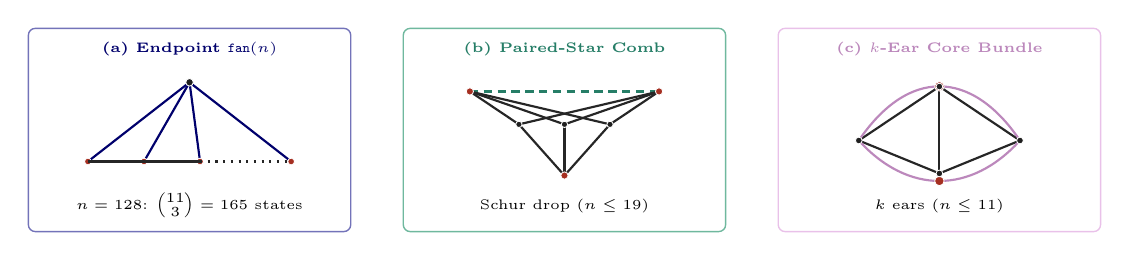
\begin{tikzpicture}[scale=0.89]
  % (a) 128-loop endpoint fan(n)
  \begin{scope}[xshift=-5.35cm]
    \draw[rounded corners=2.5pt, draw=NavyBlue!55, fill=white, line width=0.5pt] (-2.30,-1.45) rectangle (2.30,1.45);
    \node[font=\tiny\bfseries, text=NavyBlue!85!black] at (0,1.15) {(a) Endpoint $\texttt{fan}(n)$};
    \coordinate (ap) at (0,0.68);
    \foreach \idx/\xx in {0/-1.45, 1/-0.65, 2/0.15, 3/1.45} {
      \coordinate (bs\idx) at (\xx,-0.45);
      \draw[prop, NavyBlue!85!black] (ap)--(bs\idx);
      \filldraw[vbiv] (bs\idx) circle (0.048cm);
    }
    \draw[prop] (bs0)--(bs1)--(bs2);
    \draw[prop, dotted] (bs2)--(bs3);
    \filldraw[v0] (ap) circle (0.054cm);
    \node[font=\tiny] at (0,-1.08) {$n=128$: $\binom{11}{3}=165$ states};
  \end{scope}
  % (b) 19-loop passive paired-star comb
  \begin{scope}[xshift=0cm]
    \draw[rounded corners=2.5pt, draw=PineGreen!55, fill=white, line width=0.5pt] (-2.30,-1.45) rectangle (2.30,1.45);
    \node[font=\tiny\bfseries, text=PineGreen!85!black] at (0,1.15) {(b) Paired-Star Comb};
    \coordinate (ta) at (-1.35, 0.55);
    \coordinate (tb) at ( 1.35, 0.55);
    \coordinate (tc) at ( 0.00,-0.65);
    \draw[line width=0.95pt, densely dashed, draw=PineGreen!85!black] (ta)--(tb);
    \foreach \xx in {-0.65, 0.00, 0.65} {
      \coordinate (st) at (\xx,0.08);
      \draw[prop] (st)--(ta); \draw[prop] (st)--(tb); \draw[prop] (st)--(tc);
      \filldraw[v0] (st) circle (0.045cm);
    }
    \filldraw[vbiv] (ta) circle (0.052cm); \filldraw[vbiv] (tb) circle (0.052cm); \filldraw[vbiv] (tc) circle (0.052cm);
    \node[font=\tiny] at (0,-1.08) {Schur drop ($n \le 19$)};
  \end{scope}
  % (c) k-ear core bundle
  \begin{scope}[xshift=5.35cm]
    \draw[rounded corners=2.5pt, draw=Plum!65, fill=white, line width=0.5pt] (-2.30,-1.45) rectangle (2.30,1.45);
    \node[font=\tiny\bfseries, text=Plum!85!black] at (0,1.15) {(c) $k$-Ear Core Bundle};
    \coordinate (ea) at (-1.15,-0.15); \coordinate (eb) at (1.15,-0.15);
    \coordinate (ec) at (0,0.62); \coordinate (ed) at (0,-0.62);
    \draw[prop] (ea)--(ec)--(eb)--(ed)--cycle; \draw[prop] (ec)--(ed);
    \draw[prop, Plum!85!black] (ea) .. controls (-0.45,0.88) and (0.45,0.88) .. node[pos=0.5, vbiv, scale=0.78] {} (eb);
    \draw[prop, Plum!85!black] (ea) .. controls (-0.45,-0.92) and (0.45,-0.92) .. node[pos=0.5, vbiv, scale=0.78] {} (eb);
    \foreach \pt in {ea,eb,ec,ed} \filldraw[v0] (\pt) circle (0.048cm);
    \node[font=\tiny] at (0,-1.08) {$k$ ears ($n \le 11$)};
  \end{scope}
\end{tikzpicture}
\caption{All-order and high-loop tractable product-forest families of Proposition~\ref{prop:passive-comb-fan-ear}: (a)~endpoint $\texttt{fan}(n)$ evaluated at $128$ loops via $165$-state reverse spoke transfer; (b)~passive paired-star comb through $19$ loops; (c)~$k$-ear bundle over an irreducible core through $11$ loops.}
\label{fig:comb-fan-ear}
\end{figure}

\subsection{Finite Five-Loop \texorpdfstring{$K_{3,3}+e$}{K\_\{3,3\}+e} Completion and \texorpdfstring{$200/200$}{200/200} Five-Loop Forest Census}
\label{subsec:k33e-and-census}

\begin{theorem}[Finite $5$-loop $K_{3,3}+e$ evaluation, $468$-monomial $K_5-e$ currents, and $200/200$ census~{\cite{BBKP18,Repo9e833c8}}]
\label{thm:k33e-completion}
\leavevmode
\begin{enumerate}[label=(\arabic*),leftmargin=*]
  \item \emph{Exact $K_{3,3}+e$ closure via $17$ parametric annihilators:} On the $5$-loop $K_{3,3}+e$ product forest ($10{,}577$ original / $7{,}368$ scalar numerator terms compressed to $17$ $I_7$ periods), $17$ Bitoun--Bogner--Klausen--Panzer parametric annihilators~\cite{BBKP18} ($\sum_{\substack{p\in\{1,\dots,10\}\\\mathrm{edges}}}a_p\partial_p U = bU$: $3$ degree-$1$ $+ 14$ degree-$2$ on $135$-term $U$) generate $42{,}472$ rows and $1{,}039$ identities evaluating $R_{17} = +\frac{529509659453}{3990767616000} + \frac{272322049}{769824000}\zeta(3) - \frac{57527}{106920}\zeta(5)$, cancelling $+\frac{57527}{106920}\zeta(5)$ in $F_{\mathrm{old}}$ identically to yield
  \begin{equation}
  \label{eq:k33e-1187-exact}
  K_{K_{3,3}+e}(1,0;\,2,1;\,-3,-1) = \frac{1187 - 816\zeta(3)}{435456000} = \frac{1187}{435456000} - \frac{17}{9072000}\zeta(3) > 0,
  \end{equation}
  while its general $4$-source polynomial ($10$ bracket orbits in $\QQ+\QQ\zeta(3)+\QQ\zeta(5)$) factors $\frac{\langle\lambda_5,\lambda_6\rangle}{60480}$ out of $C_{\zeta(5)}$ (explaining $[\zeta(5)] = 0$ at $\lambda_5=0$).

  \item \emph{Syzygy-free $K_5-e$ current polynomial and $200/200$ five-loop census:} On the physical $5$-loop quartic forest $(01,13,02,24,05,06,35,36,45,46,56)$ reducing to $K_5-e$ (\texttt{prism} dual at $q=7,8$), top-degree syzygy $b f_{e,6} = a g_{e,6}$ ($f_{e,6}=a h_{e,5}, g_{e,6}=b h_{e,5}$) reconstructs $K(\lambda)$ ($16$ bracket monomials; benchmark $K((1,2),(3,-1),(5,3),(-9,-4)) = \frac{3327759589}{46656000} + \frac{50942017}{324000}\zeta(3) - \frac{45619}{180}\zeta(5)$) and all $11$ first-current spinors ($468$ monomials, $1{,}334$ rational coefficients) in denominator-free $\GL_2(\C)$-covariant form valid across all degenerate source frames:
  \begin{equation}
  \label{eq:k5me-covariant-current}
  \begin{aligned}
  M_{e,+\dot{a}}(\lambda) &= \sum_{\substack{p+q\le 5\\\mathrm{frame\ deg}}}\langle\lambda_1,\lambda_2\rangle^{5-p-q}\langle\lambda_5,\lambda_2\rangle^p\langle\lambda_1,\lambda_5\rangle^q\bigl(f_{e,pq}\lambda_{1,+\dot{a}} + g_{e,pq}\lambda_{2,+\dot{a}}\bigr)\\
  &\quad + \sum_{\substack{p+q=5\\\mathrm{top\ syzygy}}}\langle\lambda_5,\lambda_2\rangle^p\langle\lambda_1,\lambda_5\rangle^q h_{e,pq}\lambda_{5,+\dot{a}}.
  \end{aligned}
  \end{equation}
  Across \textbf{all $200/200$ five-loop product forests} ($2{,}200$ spinors, $4{,}400$ entries, Figure~\ref{fig:five-loop-forests}), $10$ bare kernels vanish ($10/10$ have nonzero first currents, exemplified in Table~\ref{tab:zero-marked-currents}), $107 \in \QQ$, $77 \in \QQ+\QQ\zeta(3)$, and $6 \in \QQ+\QQ\zeta(3)+\QQ\zeta(5)$.
\end{enumerate}
\end{theorem}

\begin{proof}
In~(1), integrating $\sum_{\substack{p\\\mathrm{edges}}}\partial_p(t_p^{\alpha_p}a_p U^{-q}) = 0$ on $\mathbb{RP}^9_{>0}$ yields exact rational period relations without pole shifts; $2{,}580$ pivots express $R_{17}$ in $K_{3,3}$/\texttt{prism} masters, cancelling $\zeta(5)$ and matching \texttt{ForestCubeExpansion} intervals. In~(2), comparing $\GL_2$ frames $\lambda_1=(1,0),\lambda_2=(0,1),\lambda_5=(a,b)$ and $\lambda_2=(s,t),\lambda_5=(0,1)$ at $t=0$ proves $\deg f_e,\deg g_e \le 6$ and $f_{e,6}=a h_{e,5}, g_{e,6}=b h_{e,5}$, unisolvent on $16$ symmetry-reduced integer nodes and verified independently on $((2,1),(1,2),(-1,4))$ and degenerate $((1,0),(2,0),(0,1))$.
\end{proof}

\begin{table}[H]
\centering
\scriptsize
\setlength{\tabcolsep}{6pt}
\renewcommand{\arraystretch}{1.15}
\begin{tabular}{@{}crr@{}}
\toprule
\textbf{Oriented Edge $e$} & \textbf{Coefficient $A_e$} & \textbf{Coefficient $B_e$} \\
\midrule
$0\to 1$ and $1\to 3$ & $\frac{923}{1828915200} - \frac{1}{8467200}\zeta(3) > 0$ & $\frac{17}{114307200} - \frac{1}{8467200}\zeta(3) > 0$ \\
$0\to 2$ and $2\to 4$ & $-\frac{17}{114307200} + \frac{1}{8467200}\zeta(3)$ & $-\frac{923}{1828915200} + \frac{1}{8467200}\zeta(3)$ \\
$0\to 5$ & $\frac{38987}{30481920000} - \frac{137}{105840000}\zeta(3)$ & $-\frac{38987}{30481920000} + \frac{137}{105840000}\zeta(3)$ \\
$0\to 6$ & $-\frac{49837}{30481920000} + \frac{137}{105840000}\zeta(3)$ & $\frac{49837}{30481920000} - \frac{137}{105840000}\zeta(3)$ \\
$3\to 5$ & $\frac{1597}{2612736000} - \frac{1}{6048000}\zeta(3)$ & $\frac{341}{338688000} - \frac{11}{14112000}\zeta(3)$ \\
$3\to 6$ & $-\frac{1949}{18289152000} + \frac{1}{21168000}\zeta(3)$ & $-\frac{1121}{1306368000} + \frac{1}{1512000}\zeta(3)$ \\
$4\to 5$ & $-\frac{341}{338688000} + \frac{11}{14112000}\zeta(3)$ & $-\frac{1597}{2612736000} + \frac{1}{6048000}\zeta(3)$ \\
$4\to 6$ & $\frac{1121}{1306368000} - \frac{1}{1512000}\zeta(3)$ & $\frac{1949}{18289152000} - \frac{1}{21168000}\zeta(3)$ \\
$5\to 6$ & $\frac{40393}{45722880000} - \frac{1}{1470000}\zeta(3)$ & $-\frac{40393}{45722880000} + \frac{1}{1470000}\zeta(3)$ \\
\bottomrule
\end{tabular}
\caption{Complete $11$-edge first-current spinors $M_{e,+\dot{a}}|_{\lambda_5=0} = \langle\lambda_1,\lambda_2\rangle^5(A_e\lambda_{1,+\dot{a}} + B_e\lambda_{2,+\dot{a}})$ on the five-loop $K_5-e$ quartic forest where $K|_{\lambda_5=0} \equiv 0$, obeying $\zeta(3) < \frac{5}{4} \implies A_{01} > \frac{653}{1828915200} > 0$~\cite{Repo9e833c8}.}
\label{tab:zero-marked-currents}
\end{table}

\begin{figure}[H]
\centering
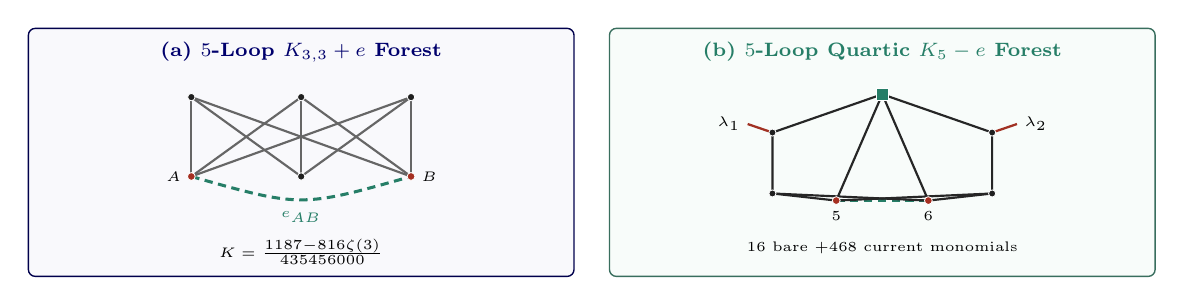
\begin{tikzpicture}[scale=0.90]
  % Left: 5-loop K_{3,3}+e product forest
  \begin{scope}[shift={(-4.10,0)}]
    \draw[rounded corners=2.5pt, draw=NavyBlue!60!black, fill=NavyBlue!2.5, line width=0.5pt] (-3.85,-1.75) rectangle (3.85,1.75);
    \node[font=\scriptsize\bfseries, text=NavyBlue!85!black] at (0,1.42) {(a) $5$-Loop $K_{3,3}+e$ Forest};
    \foreach \idx/\xx in {1/-1.55, 2/0.0, 3/1.55} {
      \coordinate (ua\idx) at (\xx, 0.78);
      \coordinate (ub\idx) at (\xx,-0.34);
    }
    \foreach \p in {1,2,3} \foreach \q in {1,2,3} \draw[prop, gray!80!black] (ua\p)--(ub\q);
    \draw[line width=1.1pt, densely dashed, draw=PineGreen!85!black] (ub1) .. controls (0,-0.78) .. node[below=0.5pt, font=\tiny, text=PineGreen!85!black] {$e_{AB}$} (ub3);
    \foreach \p in {1,2,3} \filldraw[v0] (ua\p) circle (0.052cm);
    \filldraw[vbiv] (ub1) circle (0.055cm) node[left=1pt, font=\tiny] {$A$};
    \filldraw[v0] (ub2) circle (0.052cm);
    \filldraw[vbiv] (ub3) circle (0.055cm) node[right=1pt, font=\tiny] {$B$};
    \node[font=\tiny] at (0,-1.40) {$K = \frac{1187 - 816\zeta(3)}{435456000}$};
  \end{scope}

  % Right: 5-loop K_5 - e quartic product forest
  \begin{scope}[shift={(4.10,0)}]
    \draw[rounded corners=2.5pt, draw=PineGreen!65!black, fill=PineGreen!2.5, line width=0.5pt] (-3.85,-1.75) rectangle (3.85,1.75);
    \node[font=\scriptsize\bfseries, text=PineGreen!85!black] at (0,1.42) {(b) $5$-Loop Quartic $K_5-e$ Forest};
    \coordinate (v0) at (0,0.82);
    \coordinate (v1) at (-1.55,0.28); \coordinate (v3) at (-1.55,-0.58);
    \coordinate (v2) at ( 1.55,0.28); \coordinate (v4) at ( 1.55,-0.58);
    \coordinate (v5) at (-0.65,-0.68); \coordinate (v6) at ( 0.65,-0.68);
    \draw[line width=1.1pt, densely dashed, draw=PineGreen!85!black] (v5)--(v6);
    \draw[prop] (v0)--(v1)--(v3)--(v5); \draw[prop] (v3)--(v6);
    \draw[prop] (v0)--(v2)--(v4)--(v5); \draw[prop] (v4)--(v6);
    \draw[prop] (v0)--(v5); \draw[prop] (v0)--(v6);
    \draw[extleg] (v1)--++(-0.35,0.12) node[left=-1pt, font=\tiny] {$\lambda_1$};
    \draw[extleg] (v2)--++( 0.35,0.12) node[right=-1pt, font=\tiny] {$\lambda_2$};
    \node[vi2] at (v0) {};
    \foreach \pt in {v1,v2,v3,v4} \filldraw[v0] (\pt) circle (0.05cm);
    \filldraw[vbiv] (v5) circle (0.055cm) node[below=1pt, font=\tiny] {$5$};
    \filldraw[vbiv] (v6) circle (0.055cm) node[below=1pt, font=\tiny] {$6$};
    \node[font=\tiny] at (0,-1.35) {$16$ bare $+ 468$ current monomials};
  \end{scope}
\end{tikzpicture}
\caption{Key five-loop $\C^2$ product forests completed in Theorem~\ref{thm:k33e-completion}: (a)~$K_{3,3}+e$ evaluated via $17$ parametric annihilators cancelling $\zeta(5)$; (b)~physical quartic $K_5-e$ ($\blacksquare = \Wb_4$) with $16$ bare and $468$ first-current spinor monomials across $200/200$ five-loop forests.}
\label{fig:five-loop-forests}
\end{figure}

\subsection{In-Situ \texorpdfstring{$4\mathrm{D}$}{4D} Twist Background, Open-Color \texorpdfstring{$\zeta(3)$}{zeta(3)} Cancellation, and \texorpdfstring{$4$}{4}-Loop \texorpdfstring{$\ghb^2$}{b\^2} Product}
\label{subsec:universal-quartic-product}

To evaluate multi-loop product forests of physical gauge--matter operators with nonrenormalizable superpotentials (and later $\mathcal{N}=4$ superfields in Section~\ref{sec:sugra-bcov-holo}), we now introduce in situ the off-shell four-dimensional supersymmetric twist on $\RR^4 \cong \C^2$ from scratch.

\begin{zkmodule}{Off-Shell $4\mathrm{D}$ $\mathcal{N}=1$ Twist to Holomorphic $BF$--$\beta\gamma$ and $\mathcal{N}=4$ to $\C^{2|3}$ Chern--Simons}{offshell-n1-bv-master-action}
On flat Euclidean $\RR^4 \cong \C^2$ ($\Omega := 2\,\dd x^{+\dot{+}}\wedge\dd x^{+\dot{-}}$, $\dbar := \frac{1}{2}\dd x^-_{\dot{a}}\partial_-{}^{\dot{a}}$; spinor and bispinor conventions in Appendix~\ref{app:conventions}) with compact gauge Lie algebra $\fg$, matter representation $\cR$, chiral superpotential $W(\phi) = \sum_{\substack{m\ge 2\\\mathrm{arity}}}\frac{1}{m!}W_{I_1\cdots I_m}\phi^{I_1}\cdots\phi^{I_m}$, and independent antichiral superpotential $\Wb(\bar{\phi}) = \sum_{\substack{m\ge 2\\\mathrm{arity}}}\frac{1}{m!}\Wb^{I_1\cdots I_m}\bar{\phi}_{I_1}\cdots\bar{\phi}_{I_m}$, the off-shell vector multiplet $(V_\mu{}^A, \lambda_a{}^A, \bar{\lambda}_{\dot{a}}{}^A, D^A)$ and chiral/antichiral matter $(\phi^I, \psi_a{}^I, F^I; \bar{\phi}_I, \bar{\psi}_{\dot{a}I}, \bar{F}_I)$ carry the physical Euclidean action
\begin{equation}
\label{eq:4d-offshell-euclidean-action}
\begin{aligned}
S_{E,\mathrm{phys}} = \int_{\RR^4}\dd^4x\,\Bigl[&\tfrac{1}{4}\kappa_{AB}f_{\mu\nu}{}^A f^{\mu\nu B} - \ii\kappa_{AB}\lambda^{a A}(\sigma^\mu)_{a\dot{b}}(\nabla_\mu\bar{\lambda}^{\dot{b}})^B - \tfrac{1}{2}\kappa_{AB}D^A D^B\\
&+ (\nabla_\mu\bar{\phi})_I(\nabla^\mu\phi)^I - \ii\bar{\psi}^{\dot{b}}{}_I(\bar{\sigma}^\mu)_{\dot{b}a}(\nabla_\mu\psi^a)^I - \bar{F}_I F^I\\
&+ \ii\sqrt{2}\,g\bigl(\bar{\phi}_I(t_A)^I{}_J\psi^{a J}\lambda_a{}^A - \bar{\lambda}_{\dot{a}}{}^A\bar{\psi}^{\dot{a}}{}_I(t_A)^I{}_J\phi^J\bigr) + \ii g D^A\bar{\phi}_I(t_A)^I{}_J\phi^J\\
&- F^I\partial_I W(\phi) + \tfrac{1}{2}\partial_I\partial_J W(\phi)\psi^{a I}\psi_a{}^J - \bar{F}_I\partial^{\bar{I}}\Wb(\bar{\phi}) + \tfrac{1}{2}\partial^{\bar{I}}\partial^{\bar{J}}\Wb(\bar{\phi})\bar{\psi}_{\dot{a}I}\bar{\psi}^{\dot{a}}{}_J\Bigr].
\end{aligned}
\end{equation}
Specializing the commuting supersymmetry parameter to $\xi_0{}^a = \delta^a{}_-$ ($\bar{\xi}_{0,\dot{a}} = 0$, $Q_-^2 = 0$) gives $Q_- V_{-\dot{a}}{}^A = 0$, $Q_- V_{+\dot{a}}{}^A = -2\bar{\lambda}_{\dot{a}}{}^A$, $Q_-\bar{\lambda}_{\dot{a}}{}^A = 0$, $Q_-\lambda_a{}^A = \frac{1}{2}(\sigma^{\mu\nu})_a{}^- f_{\mu\nu}{}^A + \ii\delta_a{}^- D^A$, $Q_-\bar{\phi}_I = 0$, $Q_-\phi^I = -\sqrt{2}\psi_-{}^I$, $Q_-\psi_+{}^I = -\ii\sqrt{2}\,F^I$, and $Q_-\bar{\psi}_{\dot{a}I} = -\ii\sqrt{2}(\nabla_{-\dot{a}}\bar{\phi})_I$.
\end{zkmodule}

\begin{proposition}[{First-principles off-shell BV twist to holomorphic $BF$--$\beta\gamma$ on $\C^2$ and $\C^{2|3}$ Chern--Simons~{\cite{CostelloNotes,ESW,BGKWY,LLC}}}]
\label{prop:4d-offshell-twist}
\leavevmode
\begin{enumerate}[label=(\arabic*),leftmargin=*]
  \item Adding right-placed BV antifield couplings $\int\dd^4x\,(s_{\mathrm{BRST}} + Q_-)\Phi^\Lambda\,\Phi^\ddagger_\Lambda + \mathcal{O}((\Phi^\ddagger)^2)$ to~\eqref{eq:4d-offshell-euclidean-action}, shifting $(\lambda^{\ddagger -}{}_A, \bar{F}^{\ddagger I})$ to absorb quadratic $Q_-$ terms, and integrating out the algebraic/contractible pairs $(D^A, \lambda_-{}^A)$, $(F^I, \bar{F}_I)$, and $(\phi^I, \psi_-{}^I)$ (decoupling $W(\phi)$ entirely) packages $\mathcal{A}^A \in \Omega^{0,\bullet}(\C^2)\otimes\fg[1]$, $\mathcal{B}_A \in \Omega^{2,\bullet}(\C^2)\otimes\fg^*[-1]$, $\gamma_I \in \Omega^{0,\bullet}(\C^2)\otimes\cR^*$, and $\beta^I \in \Omega^{2,\bullet}(\C^2)\otimes\cR[-1]$ into the holomorphic $BF$--$\beta\gamma$ Euclidean BV action $S_{E,\mathrm{hol}} = S_{E,\mathrm{hol,free}} + \Ihol$:
  \begin{equation}
  \label{eq:sum-Ihol}
  \begin{aligned}
  S_{E,\mathrm{hol}}[\mathcal{A},\mathcal{B},\beta,\gamma] &= \int_{\C^2}\!\left(\mathcal{B}_A\wedge\dbar\mathcal{A}^A + \beta^I\wedge\dbar\gamma_I\right)\\
  &\quad + \int_{\C^2}\!\left(\tfrac{1}{2}f^A{}_{BC}\mathcal{B}_A\wedge\mathcal{A}^B\wedge\mathcal{A}^C + \ii g(t_A)^J{}_I\beta^I\wedge\mathcal{A}^A\wedge\gamma_J + \Omega\wedge\Wb(\gamma)\right).
  \end{aligned}
  \end{equation}

  \item Specializing~\eqref{eq:sum-Ihol} to three adjoint chirals $\cR = \fg\otimes\C^3$ ($\hat{\alpha},\hat{\beta},\hat{\gamma} \in \{1,2,3\}$) with $\Wb(\gamma) = \frac{g}{6}f^{ABC}\eps^{\hat{\alpha}\hat{\beta}\hat{\gamma}}\gamma_{\hat{\alpha},A}\gamma_{\hat{\beta},B}\gamma_{\hat{\gamma},C}$ and $\boldsymbol{\mathcal{A}}^A(z,\bar{z},\theta) := \mathcal{A}^A + \theta^{\hat{\alpha}}\gamma_{\hat{\alpha}}{}^A + \frac{1}{2}\eps_{\hat{\alpha}\hat{\beta}\hat{\gamma}}\theta^{\hat{\alpha}}\theta^{\hat{\beta}}\beta^{\hat{\gamma}A} + \theta^1\theta^2\theta^3\mathcal{B}^A$ collapses~\eqref{eq:sum-Ihol} into holomorphic Chern--Simons on $\C^{2|3}$:
  \begin{equation}
  \label{eq:n4-super-hcs}
  S_{E,\mathcal{N}=4}[\boldsymbol{\mathcal{A}}] = \int_{\C^{2|3}}\Omega_{2|3}\wedge\left(\frac{1}{2}\kappa_{AB}\boldsymbol{\mathcal{A}}^A\wedge\dbar\boldsymbol{\mathcal{A}}^B + \frac{g}{6}f_{ABC}\boldsymbol{\mathcal{A}}^A\wedge\boldsymbol{\mathcal{A}}^B\wedge\boldsymbol{\mathcal{A}}^C\right).
  \end{equation}
\end{enumerate}
\end{proposition}

\begin{proof}\leavevmode
\begin{proofpart}{Part (1): Bispinor splitting and contractible doublet elimination}
From $\{Q_a,\bar{Q}_{\dot{b}}\} = -2\ii\partial_{a\dot{b}}$, $Q_- = \delta^a{}_- Q_a$ obeys $Q_-^2 = 0$ and $\{Q_-,\bar{Q}_{\dot{a}}\} = -4\ii\dbar_{\dot{a}}$. Splitting $\frac{1}{4}f_{\mu\nu}f^{\mu\nu} = \frac{1}{8}f_{ab}f^{ab} + \frac{1}{8}\bar{f}_{\dot{a}\dot{b}}\bar{f}^{\dot{a}\dot{b}}$ modulo the Pontryagin density and shifting $(\lambda^{\ddagger -}{}_A, \bar{F}^{\ddagger I})$ converts the kinetic terms into $\mathcal{B}_A\wedge\dbar\mathcal{A}^A + \beta^I\wedge\dbar\gamma_I$ ($\mathcal{A}^A = \ghc^A + \frac{1}{2}g\,\dd x^-_{\dot{a}}V_-{}^{\dot{a}A} + \cdots$, $\gamma_I = \bar{\phi}_I + \cdots$), while Gaussian/acyclic elimination of $(D^{\mathrm{shift},A},\lambda_-{}^A)$ and $(\phi^I,\psi_-{}^I)$ sets $\phi^I = \psi_-{}^I = 0$ inside $W(\phi)$, leaving~\eqref{eq:sum-Ihol}.
\end{proofpart}
\begin{proofpart}{Part (2): Berezin integration over $\theta^1\theta^2\theta^3$}
Selecting the $\theta^1\theta^2\theta^3$ top Berezin component in~\eqref{eq:n4-super-hcs} pairs $\theta^0$ with $\theta^3$ into $\mathcal{B}_A\wedge F^{0,2}(\mathcal{A})^A$, $\theta^1$ with $\theta^2$ into $\beta^{\hat{\alpha}}_A\wedge\dbar_{\mathcal{A}}\gamma_{\hat{\alpha}}{}^A$, and $(\theta^1)^3$ into $\Omega\wedge\Wb(\gamma)$ (Figure~\ref{fig:4d-twist-reduction}).
\end{proofpart}
\end{proof}

\begin{figure}[H]
\centering
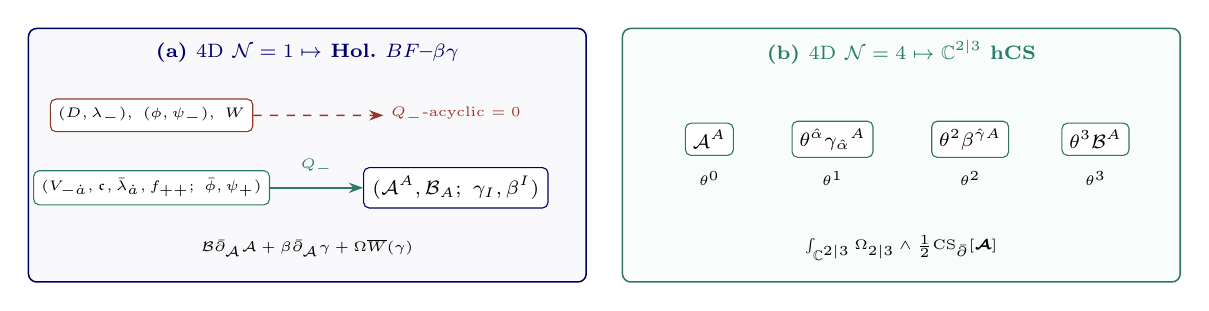
\begin{tikzpicture}[scale=0.92]
  % Left: 4D N=1 off-shell -> Holomorphic BF-betagamma
  \begin{scope}[shift={(-4.10,0)}]
    \draw[rounded corners=3pt, draw=NavyBlue!75!black, fill=NavyBlue!2.5, line width=0.55pt] (-3.85,-1.75) rectangle (3.85,1.75);
    \node[font=\scriptsize\bfseries, text=NavyBlue!85!black] at (0,1.42) {(a) $4\mathrm{D}$ $\mathcal{N}=1 \mapsto$ Hol.\ $BF$--$\beta\gamma$};
    \node[draw=BrickRed!75!black, rounded corners=2pt, fill=white, inner sep=2.8pt, font=\tiny] (ac) at (-2.15, 0.55) {$(D,\lambda_-),\ (\phi,\psi_-),\ W$};
    \node[draw=PineGreen!80!black, rounded corners=2pt, fill=white, inner sep=2.8pt, font=\tiny] (su) at (-2.15,-0.45) {$(V_{-\dot{a}},\ghc,\bar{\lambda}_{\dot{a}},f_{++};\ \bar{\phi},\psi_+)$};
    \node[draw=NavyBlue!80!black, rounded corners=2pt, fill=white, inner sep=3.2pt, font=\scriptsize] (bf) at ( 2.05,-0.45) {$(\mathcal{A}^A,\mathcal{B}_A;\ \gamma_I,\beta^I)$};
    \node[font=\tiny, text=BrickRed!85!black] at ( 2.05, 0.55) {$Q_-$-acyclic $= 0$};
    \draw[-{Stealth[length=1.8mm,width=1.3mm]}, dashed, BrickRed!80!black, line width=0.6pt] (ac) -- (1.05,0.55);
    \draw[-{Stealth[length=1.8mm,width=1.3mm]}, PineGreen!80!black, line width=0.65pt] (su) -- node[above=1pt, font=\tiny] {$Q_-$} (bf);
    \node[font=\tiny] at (0,-1.28) {$\mathcal{B}\dbar_{\mathcal{A}}\mathcal{A} + \beta\dbar_{\mathcal{A}}\gamma + \Omega\Wb(\gamma)$};
  \end{scope}

  % Right: 4D N=4 -> C^{2|3} hCS
  \begin{scope}[shift={(4.10,0)}]
    \draw[rounded corners=3pt, draw=PineGreen!75!black, fill=PineGreen!2.5, line width=0.55pt] (-3.85,-1.75) rectangle (3.85,1.75);
    \node[font=\scriptsize\bfseries, text=PineGreen!85!black] at (0,1.42) {(b) $4\mathrm{D}$ $\mathcal{N}=4 \mapsto \C^{2|3}$ hCS};
    \foreach \pp/\xx/\lbl in {
      0/-2.65/{\mathcal{A}^A},
      1/-0.95/{\theta^{\hat{\alpha}}\gamma_{\hat{\alpha}}{}^A},
      2/ 0.95/{\theta^2\beta^{\hat{\gamma}A}},
      3/ 2.68/{\theta^3\mathcal{B}^A}%
    } {
      \node[draw=PineGreen!75!black, rounded corners=2pt, fill=white, inner sep=2.6pt, font=\scriptsize] at (\xx,0.22) {$\lbl$};
      \node[font=\tiny] at (\xx,-0.32) {$\theta^{\pp}$};
    }
    \node[font=\tiny] at (0,-1.28) {$\int_{\C^{2|3}}\Omega_{2|3}\wedge\frac{1}{2}\mathrm{CS}_{\dbar}[\boldsymbol{\mathcal{A}}]$};
  \end{scope}
\end{tikzpicture}
\caption{In-situ off-shell four-dimensional BV twists (Background Card~5.1 and Proposition~\ref{prop:4d-offshell-twist}): (a)~$\mathcal{N}=1$ elimination of $Q_-$-contractible pairs and holomorphic $W(\phi)$ leaving $BF$--$\beta\gamma + \Omega\Wb(\gamma)$ on $\C^2$; (b)~$\mathcal{N}=4$ superfield assembly into holomorphic Chern--Simons on $\C^{2|3}$.}
\label{fig:4d-twist-reduction}
\end{figure}

\begin{theorem}[Universal open-color $\zeta(3)$ cancellation for all $\deg\Wb \ge 3$ and $4$-loop $\ghb^2$ product~{\cite{Repo9e833c8}}]
\label{thm:universal-quartic}
In $4\mathrm{D}$ $\mathcal{N}=1$ twisted gauge-matter theory~\eqref{eq:sum-Ihol} for \textbf{any} compact Lie algebra $\fg$ and representation $\cR$:
\begin{enumerate}[label=(\arabic*),leftmargin=*]
  \item \emph{Open-color $3$-loop quartic and arbitrary-degree pure-$\Wb$ rationality:} On $A = \beta^{1 i_1}(\partial_{+\dot{a}}\beta^{2 i_2})\gamma_5$ and $B = \ghb_A\beta^{3 i_3}$ ($\gamma_5$ neutral spectator, $[\hbar^{\ge 4}] = 0$ by $n+r \le 4$), across all $28$ Wick matchings ($12$ unreduced color words), the $16$ commutator-triple matchings on $K_4$-wheels $G_1,G_2,G_3$ concentrate the \textbf{entire} $\zeta(3)$ coefficient into the representation commutator identity
  \begin{equation}
  \label{eq:universal-commutator-zeta3}
  \mathcal{T}_{\zeta(3)} = \zeta(3)\Bigl[S^{(1)}_{+\dot{a}}(\lambda)\bigl([t_A,t_B] - \ii C^C{}_{AB}t_C\bigr)^{i_1}{}_{j_1}\Wb^{j_1 i_2 i_3 i_4} + S^{(2)}_{+\dot{a}}(\lambda)\bigl([t_A,t_B] - \ii C^C{}_{AB}t_C\bigr)^{i_2}{}_{j_2}\Wb^{i_1 j_2 i_3 i_4}\Bigr] \equiv 0,
  \end{equation}
  leaving $10$ explicit rational color words (specializing on $\mathrm{U}(1)$ at $(1,-1,0,0)$ to $\frac{g^2}{552960(8\pi^2)^3}(\partial_1\cdot\partial_2)^3(12\partial_1-19\partial_2)\gamma_4\ghc$ and on $\SU(2)$ adjoints to $-\frac{g^2}{92160(8\pi^2)^3}(\partial_1\cdot\partial_2)^3(8\partial_1+5\partial_2)\gamma_4^E\ghc_E$). The identical $16$-matching commutator mechanism cancels $\zeta(3)$ for \textbf{every pure-matter superpotential of arbitrary degree $\deg\Wb \ge 3$} ($16$ commutator $+ 8$ passive star $+ 4(\deg\Wb-3)$ SP matchings per slot-triple)!

  \item \emph{Complete $4$-loop two-antighost product:} For $\beta^1(\partial_{+\dot{a}}\beta^2)\gamma_5 \star \ghb^2\beta^3 \to \ghc\gamma_4\gamma_5$ ($324$ matchings across $14$ geometries, $7$ carrying individual $\zeta(3)$ periods; $[\hbar^{\ge 5}]=0$), all $16$ nonzero cubic charge polynomials are purely rational ($4$ vanish), evaluating at $(1,-1,0,0)$ and $\lambda_{\gamma_5}=\lambda_{\gamma_4}$ to $\frac{\ii g^3}{14745600(8\pi^2)^4}\langle\lambda_{\gamma_4},\lambda_{\ghc}\rangle^4(10\lambda_{\gamma_4,+\dot{a}} - 3\lambda_{\ghc,+\dot{a}})$.
\end{enumerate}
\end{theorem}

\begin{proof}
In~(1), fixing three contracted $\Wb$-slots $(s_1,s_2,s_3)$, the $8$ passive-star matchings and $4(\deg\Wb-3)$ SP matchings are rational individually, while the $16$ wheel matchings across $G_1$ ($e_A$ on $s_1$, $e_B$ on $s_2$), $G_2$ ($e_B$ on $s_1$, $e_A$ on $s_2$), and $G_3$ ($3$-gluon vertex $C^C{}_{AB}$ joining $s_1$ or $s_2$) share identical $\zeta(3)$ spinor polynomials $S^{(1,2)}_{+\dot{a}}(\lambda)$ weighted by $(t_A t_B - t_B t_A - \ii C^C{}_{AB}t_C) \equiv 0$, proving~\eqref{eq:universal-commutator-zeta3} without invoking color singlets or specific representations! In~(2), $21$-node exact interpolation across all $324$ matchings cancels $\zeta(3)$ across every cubic charge monomial $q_p q_l q_m$.
\end{proof}

\subsection{Arbitrary Input Derivative Jets via the Closed \texorpdfstring{$6$}{6}-Current Simplex Form}
\label{subsec:simplex-jets}

\begin{theorem}[Rationality of arbitrary simultaneous input derivative jets via closed $6$-current simplex Stokes reduction~{\cite{Repo9e833c8}}]
\label{thm:simplex-jets}
Equip $G_1, G_2, G_3$ with common fundamental chord routing $(J_{WA}, J_{WB}, J_{AB})$ on $K_4$ ($r_c \in \Delta^2_{\mathrm{source}}$ parameterizing the subdivided chord $c \in \{WA, WB, BA\}$). For any simultaneous multi-index jet $q$ on all input slots, there exists a polynomial $F_q(J)$ defining the closed $6$-form
\begin{equation}
\label{eq:closed-6current-form}
\omega_{F_q} := F_q(J_{WA}, J_{WB}, J_{AB})\,\dd^2 J_{WA}\wedge\dd^2 J_{WB}\wedge\dd^2 J_{AB},\qquad
\dd\omega_{F_q} = 0\quad \text{on }\mathrm{Time}^5\times\Delta^2_{\mathrm{source}}.
\end{equation}
Applying Stokes' theorem to the simplex homotopies joining $c = WA$ to $WB$ and $BA$ reduces $I_{G_1}[F_q] + I_{G_2}[F_q]$ and $I_{G_1}[F_q] + I_{G_3}[F_q]$ onto outer boundary chords ($\dd^2 J_{uw} = \dd^2 y_{uc} - \dd r_c\wedge\langle\lambda_{\ghc}, \dd y_{uc}\rangle$) plus the $62$ proper shrinking scale faces of $K_4$: $46$ source-independent null faces ($\equiv 0$) and $16$ polynomial SP minor faces ($6$ edges $+ 4$ triangles $+ 6$ edge-complements), proving that \textbf{every simultaneous input derivative jet evaluates in $\QQ[\lambda]$ with zero $\zeta(3)$}!
\end{theorem}

\begin{proof}
Because $\omega_{F_q}$ is a holomorphic top $(6,0)$-form in the $6$ complex coordinates $(J_{WA,\dot{\pm}}, \allowbreak J_{WB,\dot{\pm}}, \allowbreak J_{AB,\dot{\pm}})$, $\dd\omega_{F_q} = 0$ holds identically for every polynomial $F_q$. Pulling back along $\mathrm{Time}^5\times\allowbreak\Delta^1_{WA\leftrightarrow WB}$ and $\mathrm{Time}^5\times\allowbreak\Delta^1_{WA\leftrightarrow BA}$ equates $I_{G_1}+I_{G_2}$ and $I_{G_1}+I_{G_3}$ to $\int_{\partial(\mathrm{Time}^5)}\omega_{F_q}$. Every proper subset $S \subsetneq E(K_4)$ either disconnects/leaves a bridge ($46$ null faces where $\rk\dd J < 6$) or leaves an SP $K_4$-minor ($16$ faces), whose Dirichlet simplex integrals lie purely in $\QQ[\lambda]$; substituting $[t_A,t_B] - \ii C^C{}_{AB}t_C = 0$ eliminates $I_{G_1}$ cleanly in favor of rational SP boundary integrals.
\end{proof}

\begin{lemma}[{Closedness of $\Phi^*\omega_{F_q}$ and enumeration of all $62 = 46 + 16$ shrinking faces of $K_4$}]
\label{lem:k4-62-faces}
\leavevmode
\begin{enumerate}[label=(\arabic*),leftmargin=*]
  \item For every polynomial $F_q(J_{WA,\dot{\pm}}, J_{WB,\dot{\pm}}, J_{AB,\dot{\pm}})$ and smooth map $\Phi : \mathrm{Time}^5\times\Delta^2_{\mathrm{source}} \to \C^6$, the pullback $6$-form $\Phi^*\omega_{F_q}$ satisfies $\dd(\Phi^*\omega_{F_q}) = 0$.

  \item Across all $2^6 - 2 = 62$ nonempty proper subsets $S \subsetneq E(K_4)$ ($|E(K_4)| = 6$), precisely $16$ subsets ($6$ single edges, $4$ triangles, and $6$ five-edge complements) retain full $6$-current differential rank as SP minor pairs, while the remaining $46$ subsets lose differential rank and vanish identically.
\end{enumerate}
\end{lemma}

\begin{proof}\leavevmode
\begin{proofpart}{Claim 1: Holomorphic top-form closedness}
On $\C^6$ with linear coordinates $(z_1,\dots,z_6) = (J_{WA,\dot{\pm}}, J_{WB,\dot{\pm}}, J_{AB,\dot{\pm}})$, $\omega_{F_q} = F_q(z)\,\dd z_1\wedge\cdots\wedge\dd z_6$ has $\dbar F_q = 0$ and $\dd z_k\wedge(\dd z_1\wedge\cdots\wedge\dd z_6) = 0$ ($\forall\,k$), giving $\dd\omega_{F_q} = 0$ and $\dd(\Phi^*\omega_{F_q}) = \Phi^*(\dd\omega_{F_q}) = 0$.
\end{proofpart}
\begin{proofpart}{Claim 2: Subset census by cardinality $|S| \in \{1,2,3,4,5\}$}
Shrinking $t_e \to 0$ on $S \subsetneq E(K_4)$ factors $K_4$ into $K_4|_S$ (loop number $h(S)$) and $K_4/S$ (loop number $3-h(S)$), retaining full rank $6$ along $\partial(\mathrm{Time}^5)\times\Delta^1$ precisely when $K_4|_S$ is bridgeless with $|S| - 2h(S) \in \{0,1\}$: $|S|=1$ gives $6$ SP edges ($h=0$); $|S|=2$ gives $15$ null forest pairs ($h=0$, $\rk\dd J \le 5$); $|S|=3$ splits $\binom{6}{3}=20$ into $4$ SP triangles ($h=1$) plus $16$ null spanning trees ($h=0$); $|S|=4$ gives $15$ null subsets ($12$ bridged triangle-plus-edge, $3$ $4$-cycles with $|S|-2h=2$); and $|S|=5$ gives $6$ SP diamonds $K_4-e$ ($h=2$), totaling $6+4+6 = 16$ SP faces and $15+16+15 = 46$ null faces.
\end{proofpart}
\end{proof}

\begin{figure}[H]
\centering
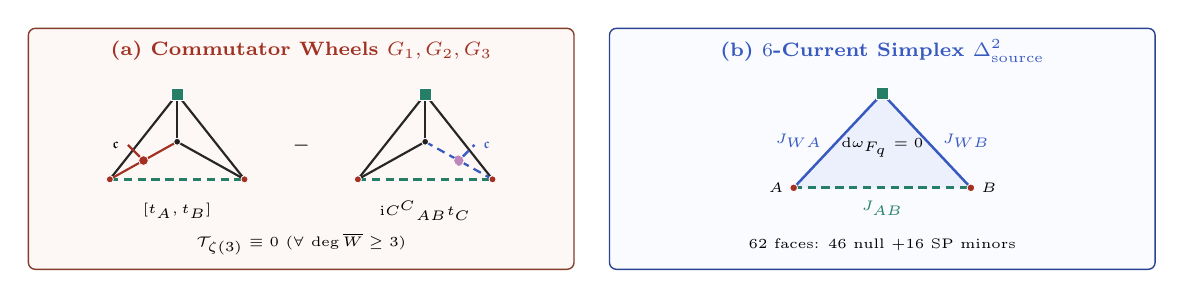
\begin{tikzpicture}[scale=0.90]
  % Left: Open-color wheel triple G1, G2, G3
  \begin{scope}[shift={(-4.10,0)}]
    \draw[rounded corners=2.5pt, draw=BrickRed!65!black, fill=BrickRed!2.5, line width=0.5pt] (-3.85,-1.70) rectangle (3.85,1.70);
    \node[font=\scriptsize\bfseries, text=BrickRed!85!black] at (0,1.38) {(a) Commutator Wheels $G_1, G_2, G_3$};
    % G1+G2
    \begin{scope}[shift={(-1.75,0.05)}]
      \coordinate (x0) at (0,0.72); \coordinate (x1) at (0,0.05);
      \coordinate (xa) at (-0.95,-0.48); \coordinate (xb) at (0.95,-0.48);
      \draw[line width=1.0pt, densely dashed, draw=PineGreen!85!black] (xa)--(xb);
      \draw[prop] (x0)--(xa); \draw[prop] (x0)--(xb); \draw[prop] (x0)--(x1); \draw[prop] (x1)--(xb);
      \draw[prop, BrickRed!85!black] (x1) -- node[vbiv, scale=0.8] (xc) {} (xa);
      \draw[extleg] (xc)--++(-0.22,0.22) node[left=-1pt, font=\tiny] {$\ghc$};
      \node[vi2] at (x0) {}; \filldraw[v0] (x1) circle (0.048cm);
      \filldraw[vbiv] (xa) circle (0.05cm); \filldraw[vbiv] (xb) circle (0.05cm);
      \node[font=\tiny] at (0,-0.92) {$[t_A, t_B]$};
    \end{scope}
    \node[font=\scriptsize\bfseries] at (0,0.05) {$-$};
    % G3
    \begin{scope}[shift={(1.75,0.05)}]
      \coordinate (y0) at (0,0.72); \coordinate (y1) at (0,0.05);
      \coordinate (ya) at (-0.95,-0.48); \coordinate (yb) at (0.95,-0.48);
      \draw[line width=1.0pt, densely dashed, draw=PineGreen!85!black] (ya)--(yb);
      \draw[prop] (y0)--(ya); \draw[prop] (y0)--(yb); \draw[prop] (y0)--(y1); \draw[prop] (y1)--(ya);
      \draw[cprop] (y1) -- node[vtcent, scale=0.78] (yg) {} (yb);
      \draw[cextleg] (yg)--++(0.22,0.22) node[right=-1pt, font=\tiny, text=RoyalBlue!85!black] {$\ghc$};
      \node[vi2] at (y0) {}; \filldraw[v0] (y1) circle (0.048cm);
      \filldraw[vbiv] (ya) circle (0.05cm); \filldraw[vbiv] (yb) circle (0.05cm);
      \node[font=\tiny] at (0,-0.92) {$\ii C^C{}_{AB}t_C$};
    \end{scope}
    \node[font=\tiny] at (0,-1.35) {$\mathcal{T}_{\zeta(3)} \equiv 0$ ($\forall\,\deg\Wb \ge 3$)};
  \end{scope}

  % Right: Closed 6-current simplex form on K_4
  \begin{scope}[shift={(4.10,0)}]
    \draw[rounded corners=2.5pt, draw=RoyalBlue!65!black, fill=RoyalBlue!2.5, line width=0.5pt] (-3.85,-1.70) rectangle (3.85,1.70);
    \node[font=\scriptsize\bfseries, text=RoyalBlue!85!black] at (0,1.38) {(b) $6$-Current Simplex $\Delta^2_{\mathrm{source}}$};
    \coordinate (sw) at (0,0.78);
    \coordinate (sa) at (-1.25,-0.55);
    \coordinate (sb) at ( 1.25,-0.55);
    \fill[RoyalBlue!10] (sw)--(sa)--(sb)--cycle;
    \draw[prop, RoyalBlue!85!black, line width=0.9pt] (sw) -- node[left=2pt, font=\tiny] {$J_{WA}$} (sa);
    \draw[prop, RoyalBlue!85!black, line width=0.9pt] (sw) -- node[right=2pt, font=\tiny] {$J_{WB}$} (sb);
    \draw[line width=1.05pt, densely dashed, draw=PineGreen!85!black] (sa) -- node[below=1pt, font=\tiny, text=PineGreen!85!black] {$J_{AB}$} (sb);
    \node[vi2] at (sw) {};
    \filldraw[vbiv] (sa) circle (0.054cm) node[left=1pt, font=\tiny] {$A$};
    \filldraw[vbiv] (sb) circle (0.054cm) node[right=1pt, font=\tiny] {$B$};
    \node[font=\tiny] at (0,0.02) {$\dd\omega_{F_q} = 0$};
    \node[font=\tiny] at (0,-1.35) {$62$ faces: $46$ null $+ 16$ SP minors};
  \end{scope}
\end{tikzpicture}
\caption{Mechanisms of Theorems~\ref{thm:universal-quartic} and~\ref{thm:simplex-jets}: (a)~representation-commutator triple $G_1,G_2,G_3$ cancelling $\zeta(3)$ for arbitrary gauge group and $\deg\Wb \ge 3$; (b)~closed $6$-current form $\omega_{F_q}$ on $\mathrm{Time}^5\times\Delta^2_{\mathrm{source}}$ reducing arbitrary simultaneous derivative jets to $16$ rational SP boundary minors.}
\label{fig:open-color-and-simplex}
\end{figure}

% ============================================================================
\section{Commutative \texorpdfstring{$5\mathrm{D}$}{5D}, \texorpdfstring{$9\mathrm{D}$}{9D}, and \texorpdfstring{$10\mathrm{D}$}{10D} Chern--Simons Quantization and Multi-Loop \texorpdfstring{$2\mathrm{D}$--$8\mathrm{D}$}{2D--8D} Gauge Cohomology}
\label{sec:cs-gauge-twists}
% ============================================================================

Having developed the $(H,T)$ Schwinger period and forest engines in Sections~\ref{sec:schwinger-periods-k5}--\ref{sec:forests-quartic-jets}, we now analyze multi-loop quantization and anomalies across five-, nine-, and ten-dimensional Chern--Simons theories and two- to eight-dimensional gauge twists~\cite{Costello16,CDG20,ESW,GKW,Repo9e833c8}. Following the proximity principle, each concrete background module enters at the exact point where the calculation invokes it: (i)~Chern--Weil transgression, finite large gauge transformations with exact Wess--Zumino winding $N_W[g]\in\ZZ$, and AKSZ superconnections open the Chern--Simons analysis; (ii)~after evaluating the two-loop $5\mathrm{D}$ Chern--Simons Feynman diagrams $\theta(1,3,3)$ and $\theta(2,2,3)$, Chevalley--Whitehead rigidity and Vogel's split-Casimir ladder plane enter directly at the Lie color contraction step; and (iii)~the Elliott--Safronov--Williams pure-spinor twist taxonomy enters right ahead of the $2\mathrm{D}$--$8\mathrm{D}$ gauge supercharge theorems.

\subsection{In-Situ TQFT Background: Chern--Weil Transgression, Exact Winding \texorpdfstring{$N_W[g]\in\ZZ$}{N\_W[g] in Z}, and AKSZ Collapse}
\label{subsec:cs-aksz-lecture}

\begin{zkmodule}{Witten vs.\ Schwarz TQFTs, Chern--Weil Transgression of $\mathrm{CS}_{2k+1}$, and AKSZ Collapse}{aksz-superconnection-ht-cs-ladder}
Topological quantum field theories separate into \emph{cohomological (Witten-type) TQFTs}---where the stress-energy tensor is $Q$-exact, $T_{\mu\nu} = \{Q, G_{\mu\nu}\}$---and \emph{Schwarz-type TQFTs}~\cite{Witten89}, whose classical action is written purely with exterior wedge products without any background metric $g_{\mu\nu}$ (a metric enters solely inside the BV gauge-fixing codifferential $D^*$ of~\eqref{eq:dstar-definition}).

\paragraph{1.\ Collision-free Lie indices and step-by-step Chern--Weil transgression of $\mathrm{CS}_3$ and $\mathrm{CS}_5$.}
Let $\fg$ have basis $T_A$ indexed by uppercase abstract Lie-algebra slots $A, B, C, E$ ($[T_B, T_C] = f^A{}_{BC}T_A$, $f_{ABC} := \kappa_{AE}f^E{}_{BC}$), and let $A = A^A T_A \in \Omega^1(M;\fg)$ be a connection $1$-form with Lie-bracket $2$-form $[A, A]^A := f^A{}_{BC}A^B\wedge A^C$ and curvature $2$-form $F^A := \dd A^A + \frac{1}{2}f^A{}_{BC}A^B\wedge A^C$. To avoid any visual collision between the connection $1$-form $A$ and the Lie-algebra slot $A$, we denote the exterior covariant derivative by $\dd_\nabla$, acting on $\eta = \eta^A T_A \in \Omega^p(M;\fg)$ by
\begin{equation}
\label{eq:covariant-d-nabla}
(\dd_\nabla\eta)^A := \dd\eta^A + f^A{}_{BC}A^B\wedge\eta^C,\qquad
(\dd_\nabla F)^A = \dd F^A + f^A{}_{BC}A^B\wedge F^C = 0\quad (\text{Bianchi identity}),
\end{equation}
with infinitesimal gauge transformation locked to the minus-sign convention
\begin{equation}
\label{eq:gauge-var-minus-dnabla}
\delta_\epsilon A^A := -(\dd_\nabla\epsilon)^A = -\bigl(\dd\epsilon^A + f^A{}_{BC}A^B\epsilon^C\bigr)\qquad \bigl(\epsilon = \epsilon^A T_A \in \Omega^0(M;\fg)\bigr).
\end{equation}
For any $\ad$-invariant symmetric polynomial $P \in (\Sym^{k+1}\fg^*)^{\fg}$ ($k \ge 1$), the Bianchi identity~\eqref{eq:covariant-d-nabla} gives $\dd P(F^{\wedge(k+1)}) = 0$. Along the linear connection path $A_s := sA$ ($s \in [0,1]$, covariant derivative $\dd_{\nabla_s} := \dd + s[A, -]$), the path curvature and velocity are
\begin{equation}
\label{eq:Fs-linear-path}
F_s^A = s\,\dd A^A + \frac{s^2}{2}[A, A]^A,\qquad
\partial_s F_s^A = \dd A^A + s[A, A]^A = (\dd_{\nabla_s}A)^A,
\end{equation}
so $\partial_s P(F_s^{\wedge(k+1)}) = (k+1)P(\dd_{\nabla_s}A, F_s^{\wedge k}) = (k+1)\dd P(A, F_s^{\wedge k})$ (using $\dd F_s = -s[A, F_s]$ and $\ad$-invariance of $P$). Integrating over $s \in [0,1]$ constructs the \emph{Chern--Simons $(2k+1)$-form}:
\begin{equation}
\label{eq:chern-weil-transgression}
\mathrm{CS}_{2k+1}[A] := (k+1)\int_0^1 \dd s\; P\!\bigl(A,\, F_s^{\wedge k}\bigr),\qquad
\dd\,\mathrm{CS}_{2k+1}[A] = P\!\bigl(F^{\wedge(k+1)}\bigr).
\end{equation}
Substituting $F_s^B = s\,\dd A^B + \frac{s^2}{2}[A,A]^B$ directly into~\eqref{eq:chern-weil-transgression} exhibits the numerical coefficients at $k = 1$ and $k = 2$ step by step:
\begin{itemize}[leftmargin=*]
  \item \textbf{At $k = 1$ ($P_2(X,Y) = \kappa_{AB}X^A Y^B$):} Integrating $2\int_0^1 s\,\dd s = 1$ and $2\int_0^1\frac{s^2}{2}\,\dd s = \frac{1}{3}$ yields
  \begin{equation}
  \label{eq:cs3-explicit}
  \tfrac{1}{2}\mathrm{CS}_3[A] = \int_0^1\dd s\,\kappa_{AB}A^A\wedge\Bigl(s\,\dd A^B + \tfrac{s^2}{2}[A,A]^B\Bigr) = \tfrac{1}{2}\kappa_{AB}A^A\wedge\dd A^B + \tfrac{1}{6}f_{ABC}A^A\wedge A^B\wedge A^C.
  \end{equation}
  \item \textbf{At $k = 2$ ($P_3(X,Y,Z) = \frac{1}{2}d_{ABC}X^A Y^B Z^C = \tr(X Y Z)|_{\mathrm{sym}} \in (\Sym^3\fg^*)^{\fg}$, where $d_{ABC} := \tr(T_A\{T_B,T_C\})$ satisfies $P_3(X,X,X) = \tr(X^3)$):} Because the $2$-forms $\dd A^B$ and $[A,A]^C$ have even exterior degree, they \emph{commute} under $\wedge$, and $d_{ABC} = d_{ACB}$ is symmetric in $(B,C)$, so the two $s^3$ cross terms $\frac{s^3}{2} + \frac{s^3}{2} = s^3$ \emph{add}:
  \[
  P_3(A, F_s, F_s) = \frac{1}{2}d_{ABC}A^A\wedge\Bigl(s^2\,\dd A^B\wedge\dd A^C + s^3\,[A,A]^B\wedge\dd A^C + \frac{s^4}{4}[A,A]^B\wedge[A,A]^C\Bigr).
  \]
  Multiplying by $(k+1) = 3$, integrating $3\int_0^1 s^2\,\dd s = 1$, $3\int_0^1 s^3\,\dd s = \frac{3}{4}$, and $3\int_0^1\frac{s^4}{4}\,\dd s = \frac{3}{20}$, and commuting $1$-forms past $2$-forms ($A^A\wedge[A,A]^B = [A,A]^B\wedge A^A$) produces the exact coefficients $(1, \frac{3}{4}, \frac{3}{20})$ (equivalently $\tr(A(\dd A)^2 + \frac{3}{2}A^3\dd A + \frac{3}{5}A^5)$ in matrix wedge notation):
  \begin{equation}
  \label{eq:cs5-explicit}
  \mathrm{CS}_5[A] = \frac{1}{2}d_{ABC}\!\left(A^A\wedge\dd A^B\wedge\dd A^C + \frac{3}{4}[A,A]^A\wedge A^B\wedge\dd A^C + \frac{3}{20}[A,A]^A\wedge[A,A]^B\wedge A^C\right).
  \end{equation}
\end{itemize}

\paragraph{2.\ $5\mathrm{D}$ HT Chern--Simons vs.\ topological $\mathrm{CS}_5$, and explicit definition of $F_D[\mathcal{A}]$.}
Whereas $3\mathrm{D}$ Chern--Simons on $M_3$ has quantized integer level $\kappa_{\mathrm{CS}} \in \ZZ$ governed by the exact Wess--Zumino winding number $N_W[g] \in \ZZ$ (Proposition~\ref{prop:cs3-large-gauge-nw}) and $4\mathrm{D}$ Costello--Witten--Yamazaki Chern--Simons on $\RR^2\times\C$~\cite{CWY18} wedges $\dd z$ with $\mathrm{CS}_3$ at $(H,T)=(1,2)$ (where all bulk loops vanish by $\rho_n(M)^{\wedge 2} = 0$), \emph{commutative $5\mathrm{D}$ HT Chern--Simons} on $\RR_\tau\times\C^2_z$ ($\Omega := \dd z^1\wedge\dd z^2$) wedges $\Omega$ with $\mathrm{CS}_3[\mathcal{A}]$ along $(\tau,\bar{z}^{\bar{1}},\bar{z}^{\bar{2}})$ using the quadratic form $\kappa_{AB}$ (defined for every Lie algebra with invariant $\kappa_{AB}$). By contrast, for $\fg = \fsl_N$ ($N \ge 3$) with symmetric cubic trace tensor $d_{ABC} := \tr(T_A\{T_B,T_C\})$ ($d_{ABC} = 0$ on $\fsl_2$), the alternating holomorphic-jet $3$-cochain $D(X_0\ee^{p^{(0)}\cdot z}, X_1\ee^{p^{(1)}\cdot z}, X_2\ee^{p^{(2)}\cdot z}) := (p^{(0)}_1 p^{(1)}_2 - p^{(0)}_2 p^{(1)}_1)d_{ABC}X_0^A X_1^B X_2^C$ ($p^{(0)}+p^{(1)}+p^{(2)}=0$) defines on $\mathcal{A}^A \in \Omega^\bullet(\RR_\tau)\widehat{\otimes}\Omega^{0,\bullet}(\C^2_z)\otimes\fg[1]$ the position-space local cubic functional
\begin{equation}
\label{eq:FD-explicit-definition}
F_D[\mathcal{A}] := \frac{1}{3}\int_{\RR\times\C^2}\dd z^1\wedge\dd z^2\wedge d_{ABC}\,(\partial_{z^1}\mathcal{A}^A)\wedge(\partial_{z^2}\mathcal{A}^B)\wedge\mathcal{A}^C,
\end{equation}
which equals $-\frac{1}{3}$ times the restriction of topological $\int_{\RR\times\C^2}\mathrm{CS}_5[\mathcal{A}]$ to $\Omega^\bullet(\RR_\tau)\widehat{\otimes}\Omega^{0,\bullet}(\C^2_z)$ (Proposition~\ref{prop:cs5-transgression-fd}) and supplies the one-loop anomaly-cancelling counterterm $J_1 = a F_D[\mathcal{A}]$ in Subsection~\ref{subsec:5d-cs-flagship}!
\end{zkmodule}

\begin{proposition}[{Finite large gauge transformation of $\frac{1}{2}\mathrm{CS}_3[A]$, exact Wess--Zumino winding number $N_W[g] \in \ZZ$, and level quantization $\kappa_{\mathrm{CS}} \in \ZZ$~{\cite{Bott59,Witten89}}}]
\label{prop:cs3-large-gauge-nw}
Let $G$ be a compact, connected, simple, simply connected Lie group with Lie algebra $\fg$, dual Coxeter number $h^\vee$, canonical basic $\Ad_G$-invariant bilinear form $\kappa^{\mathrm{norm}}_{AB} := \frac{1}{2h^\vee}\kappa^{\mathrm{Kill}}_{AB}$ normalized so long roots satisfy $(\theta_{\max},\theta_{\max})_{\mathrm{norm}} = 2$ (equivalently $\kappa^{\mathrm{norm}}(X,Y) = \tr_{\C^N}(X Y)$ on $\fg_{\C} = \fsl_N(\C)$ for $G = \SU(N)$), and smooth map $g : M_3 \to G$ on an oriented $3$-manifold $M_3$ with left-invariant Maurer--Cartan $1$-form $\theta_g := g^{-1}\dd g \in \Omega^1(M_3;\fg)$ obeying $\dd\theta_g = -\frac{1}{2}[\theta_g,\theta_g]$.
\begin{enumerate}[label=(\arabic*),leftmargin=*]
  \item \emph{Exact local $3$-form transformation aligned with $\delta_\epsilon A = -\dd_\nabla\epsilon$:} Under the finite gauge action $\dd + A^g := g(\dd + A)g^{-1}$, namely
  \begin{equation}
  \label{eq:finite-gauge-Ag}
  A^g := g A g^{-1} - (\dd g)g^{-1} = g(A - \theta_g)g^{-1}
  \quad\Bigl(g = \exp(+\epsilon) \implies \delta_\epsilon A = -(\dd\epsilon + [A,\epsilon]) = -\dd_\nabla\epsilon\Bigr),
  \end{equation}
  any $\Ad_G$-invariant symmetric bilinear form $\kappa$ on $\fg$ satisfies identically
  \begin{equation}
  \label{eq:cs3-finite-shift-exact}
  \frac{1}{2}\mathrm{CS}_3[A^g] - \frac{1}{2}\mathrm{CS}_3[A] = -\frac{1}{2}\,\dd\,\kappa\bigl(g A g^{-1},\, (\dd g)g^{-1}\bigr) + \frac{1}{12}\,\kappa\bigl(\theta_g,\, [\theta_g, \theta_g]\bigr),
  \end{equation}
  where $\kappa(g A g^{-1}, (\dd g)g^{-1}) = \kappa(A, \theta_g)$ (whereas parameterizing via the inverse map $h := g^{-1}$ with $A^{[h]} = h^{-1}A h + \theta_h$ flips the Wess--Zumino sign to $-\frac{1}{12}\kappa(\theta_h,[\theta_h,\theta_h])$).

  \item \emph{Exact Wess--Zumino winding number $N_W[g] \in \ZZ$:} For every closed oriented $3$-manifold $M_3$ ($\partial M_3 = \varnothing$) and smooth map $g : M_3 \to G$, the \textbf{Wess--Zumino winding number}
  \begin{equation}
  \label{eq:exact-NW-formula}
  N_W[g] := \frac{1}{48\pi^2}\int_{M_3}\kappa^{\mathrm{norm}}\bigl(\theta_g,\, [\theta_g, \theta_g]\bigr) = \frac{1}{96\pi^2 h^\vee}\int_{M_3}\kappa^{\mathrm{Kill}}\bigl(\theta_g,\, [\theta_g, \theta_g]\bigr) \in \ZZ
  \end{equation}
  takes exact integer values, simplifying on $G = \SU(N)$ ($[\theta_g,\theta_g] = 2\theta_g\wedge_{\mathrm{mat}}\theta_g$) to
  \begin{equation}
  \label{eq:exact-NW-suN}
  N_W[g] = \frac{1}{24\pi^2}\int_{M_3}\tr_{\C^N}\!\Bigl(\bigl(g^{-1}\dd g\bigr)^{\wedge 3}\Bigr) \in \ZZ,
  \end{equation}
  normalized to $N_W[\id_{S^3}] = +1$ on the orientation-preserving diffeomorphism $S^3 \xrightarrow{\cong} \SU(2)$.

  \item \emph{Chern--Simons action shift and integer level quantization:} On closed $M_3$, the physical Chern--Simons action $S_{L,\mathrm{CS}_3}[A] := \frac{\kappa_{\mathrm{CS}}}{2\pi}\int_{M_3}\frac{1}{2}\mathrm{CS}_3^{\mathrm{norm}}[A]$ (equal on $\SU(N)$ to $\frac{\kappa_{\mathrm{CS}}}{4\pi}\int_{M_3}\tr_{\C^N}(A\wedge\dd A + \frac{2}{3}A^{\wedge 3})$, with $S_E = -\ii S_L$) transforms by
  \begin{equation}
  \label{eq:cs3-action-shift-quant}
  \int_{M_3}\tfrac{1}{2}\mathrm{CS}_3^{\mathrm{norm}}[A^g] - \int_{M_3}\tfrac{1}{2}\mathrm{CS}_3^{\mathrm{norm}}[A] = 4\pi^2 N_W[g],\qquad
  S_{L,\mathrm{CS}_3}[A^g] - S_{L,\mathrm{CS}_3}[A] = 2\pi\,\kappa_{\mathrm{CS}}\,N_W[g],
  \end{equation}
  rendering $\exp(\ii S_{L,\mathrm{CS}_3}[A]/\hbar) = \exp(-S_{E,\mathrm{CS}_3}[A]/\hbar)$ ($\hbar = 1$) gauge-invariant across all homotopy sectors $\pi_3(G) \cong \ZZ$ precisely when $\kappa_{\mathrm{CS}} \in \ZZ$.
\end{enumerate}
\end{proposition}

\begin{proof}\leavevmode
\begin{proofpart}{Part (1): Step-by-step local $3$-form algebra and flat-connection sign verification}
Differentiating $g^{-1}g = \mathbf{1}$ gives $(\dd g^{-1})g + g^{-1}\dd g = 0 \implies \dd g^{-1} = -\theta_g g^{-1}$, hence $\dd\theta_g = (\dd g^{-1})\wedge_{\mathrm{mat}}\dd g = -\theta_g\wedge_{\mathrm{mat}}\theta_g = -\frac{1}{2}[\theta_g,\theta_g]$ (since $[X,Y]^A = f^A{}_{BC}X^B\wedge Y^C = (X\wedge_{\mathrm{mat}}Y + Y\wedge_{\mathrm{mat}}X)^A$ gives $[X,X] = 2X\wedge_{\mathrm{mat}}X$ on $1$-forms). Setting $B := A - \theta_g \in \Omega^1(M_3;\fg)$ so $A^g = g B g^{-1}$, the graded Leibniz rule on $\dd((g B)g^{-1}) = \dd(g B)g^{-1} - g B\wedge_{\mathrm{mat}}\dd g^{-1}$ gives
\[
\begin{aligned}
\dd A^g &= g\bigl(\dd B + \theta_g\wedge_{\mathrm{mat}}B + B\wedge_{\mathrm{mat}}\theta_g\bigr)g^{-1} = g\bigl(\dd B + [\theta_g, B]\bigr)g^{-1}\\
&= g\Bigl(\dd A + [\theta_g, A] - \frac{1}{2}[\theta_g,\theta_g]\Bigr)g^{-1},
\end{aligned}
\]
using $-\dd\theta_g - [\theta_g,\theta_g] = (\frac{1}{2} - 1)[\theta_g,\theta_g] = -\frac{1}{2}[\theta_g,\theta_g]$. By $\Ad_G$-invariance $\kappa(g X g^{-1}, g Y g^{-1}) = \kappa(X,Y)$ and total symmetry of $\kappa(X,[Y,Z]) = f_{ABC}X^A\wedge Y^B\wedge Z^C$ on $1$-forms $X,Y,Z$:
\[
\begin{aligned}
\tfrac{1}{2}\kappa(A^g, \dd A^g) &= \tfrac{1}{2}\kappa(A,\dd A) + \tfrac{1}{2}\kappa(A,[\theta_g,A]) - \tfrac{1}{4}\kappa(A,[\theta_g,\theta_g])\\
&\quad - \tfrac{1}{2}\kappa(\theta_g,\dd A) - \tfrac{1}{2}\kappa(\theta_g,[\theta_g,A]) + \tfrac{1}{4}\kappa(\theta_g,[\theta_g,\theta_g]),\\
\tfrac{1}{6}\kappa(A^g, [A^g,A^g]) &= \tfrac{1}{6}\kappa(A,[A,A]) - \tfrac{1}{2}\kappa(\theta_g,[A,A]) + \tfrac{1}{2}\kappa(A,[\theta_g,\theta_g]) - \tfrac{1}{6}\kappa(\theta_g,[\theta_g,\theta_g]).
\end{aligned}
\]
Summing both expansions: (i)~the $\theta_g A^2$ terms $+\frac{1}{2}\kappa(A,[\theta_g,A]) - \frac{1}{2}\kappa(\theta_g,[A,A]) = 0$ cancel; (ii)~the $A\theta_g^2$ terms combine as $(-\frac{1}{4}-\frac{1}{2}+\frac{1}{2})\kappa(A,[\theta_g,\theta_g]) = -\frac{1}{4}\kappa(A,-2\,\dd\theta_g) = +\frac{1}{2}\kappa(A,\dd\theta_g)$, which adds to $-\frac{1}{2}\kappa(\theta_g,\dd A) = -\frac{1}{2}\kappa(\dd A,\theta_g)$ (even degree $2\cdot 1 = 2$) via $\dd\kappa(A,\theta_g) = \kappa(\dd A,\theta_g) - \kappa(A,\dd\theta_g)$ to give $-\frac{1}{2}\dd\kappa(A,\theta_g) = -\frac{1}{2}\dd\kappa(g A g^{-1},(\dd g)g^{-1})$; and (iii)~the cubic $\theta_g^3$ terms combine as $(\frac{1}{4}-\frac{1}{6})\kappa(\theta_g,[\theta_g,\theta_g]) = +\frac{1}{12}\kappa(\theta_g,[\theta_g,\theta_g])$, proving~\eqref{eq:cs3-finite-shift-exact}! As an immediate consistency check at $A = 0$, pure gauge $A^g = -(\dd g)g^{-1} = -g\theta_g g^{-1}$ is flat ($F(A^g) = \dd A^g + \frac{1}{2}[A^g,A^g] = 0 \implies \dd A^g = -\frac{1}{2}[A^g,A^g]$), so $\frac{1}{2}\mathrm{CS}_3[A^g]|_{A=0} = (-\frac{1}{4}+\frac{1}{6})\kappa(A^g,[A^g,A^g]) = -\frac{1}{12}\kappa(-\theta_g,[-\theta_g,-\theta_g]) = +\frac{1}{12}\kappa(\theta_g,[\theta_g,\theta_g])$.
\end{proofpart}
\begin{proofpart}{Part (2): Explicit evaluation of $N_W[\id_{S^3}] = +1$ on $\SU(2)$ and integrality across simple $G$}
Identify the unit $3$-sphere $S^3 = \{(x^0,x^1,x^2,x^3) \in \RR^4 : \sum_{\substack{m\in\{0,1,2,3\}\\\mathrm{coords}}}(x^m)^2 = 1\}$ (oriented as $\partial B^4$, so at the north pole $p_N = (1,0,0,0)$ with outward normal $\partial_{x^0}$, $\dd\vol_{S^3}|_{p_N} = \dd x^1\wedge\dd x^2\wedge\dd x^3$) with $\SU(2)$ via $g(x) := x^0\mathbf{1}_2 + \ii(x^1\sigma_1 + x^2\sigma_2 + x^3\sigma_3)$. At $p_N$ ($g(p_N)=\mathbf{1}_2$, $\dd x^0|_{p_N}=0$), $\theta_g|_{p_N} = \ii(\sigma_1\dd x^1 + \sigma_2\dd x^2 + \sigma_3\dd x^3)$. Summing over all $3! = 6$ permutations $\pi \in S_3$ with $\sigma_{\pi(1)}\sigma_{\pi(2)}\sigma_{\pi(3)} = \sgn(\pi)\sigma_1\sigma_2\sigma_3 = \sgn(\pi)\ii\mathbf{1}_2$ and $\dd x^{\pi(1)}\wedge\dd x^{\pi(2)}\wedge\dd x^{\pi(3)} = \sgn(\pi)\dd\vol_{S^3}|_{p_N}$ yields
\[
\theta_g^{\wedge 3}\Big|_{p_N} = \ii^3\cdot 6\,(\ii\mathbf{1}_2)\,\dd\vol_{S^3}\Big|_{p_N} = +6\,\mathbf{1}_2\,\dd\vol_{S^3}\Big|_{p_N}\quad\Longrightarrow\quad
\tr_{\C^2}\!\bigl(\theta_g^{\wedge 3}\bigr)\Big|_{p_N} = +12\,\dd\vol_{S^3}\Big|_{p_N}.
\]
Because left multiplication $g \mapsto h g$ ($h \in \SU(2)$) preserves both $\theta_g = g^{-1}\dd g$ and the round metric $\dd s^2_{S^3} = -\frac{1}{2}\tr_{\C^2}(\theta_g^2)$, the equality $\tr_{\C^2}(\theta_g^{\wedge 3}) = 12\,\dd\vol_{S^3}$ (and $\kappa^{\mathrm{norm}}(\theta_g,[\theta_g,\theta_g]) = 2\tr_{\C^2}(\theta_g^{\wedge 3}) = 24\,\dd\vol_{S^3}$) holds pointwise across $S^3$. Multiplying by $\vol(S^3) = \frac{2\pi^2}{\Gamma(2)} = 2\pi^2$ gives
\[
\begin{aligned}
\int_{S^3}\tr_{\C^2}\!\bigl(\theta_g^{\wedge 3}\bigr) &= 12\cdot 2\pi^2 = 24\pi^2,\\
\int_{S^3}\kappa^{\mathrm{norm}}\bigl(\theta_g,\, [\theta_g, \theta_g]\bigr) &= 24\cdot 2\pi^2 = 48\pi^2\quad\Longrightarrow\quad N_W[\id_{S^3}] = +1!
\end{aligned}
\]
For arbitrary compact, connected, simple, simply connected $G$, Bott's theorem~\cite{Bott59} establishes $\pi_3(G) \cong \ZZ$ generated by the long-root subgroup $\iota_{\theta_{\max}} : \SU(2)_{\theta_{\max}} \hookrightarrow G$ ($(\theta_{\max},\theta_{\max})_{\mathrm{norm}} = 2$), along which $\iota_{\theta_{\max}}^*\kappa^{\mathrm{norm}}_G = \kappa^{\mathrm{norm}}_{\SU(2)}$. Because the Cartan $3$-form $\Omega_3^{\mathrm{WZ}} := \frac{1}{48\pi^2}\kappa^{\mathrm{norm}}(\theta_G,[\theta_G,\theta_G]) \in \Omega^3(G)$ is closed ($\dd\Omega_3^{\mathrm{WZ}} = 0$ by Jacobi) and integrates to $+1$ on the generator $[S^3] \in \pi_3(G) \cong H_3(G;\ZZ)$ (since $\pi_1(G)=\pi_2(G)=0$ implies $H_3(G;\ZZ) \cong \pi_3(G)$ by Hurewicz's theorem), $[\Omega_3^{\mathrm{WZ}}] \in H^3(G;\ZZ)$ is an integral cohomology class, proving $N_W[g] = \int_{M_3}g^*\Omega_3^{\mathrm{WZ}} = \langle g^*[\Omega_3^{\mathrm{WZ}}], [M_3]\rangle \in \ZZ$ for every closed oriented $3$-manifold $M_3$ and smooth map $g : M_3 \to G$.
\end{proofpart}
\begin{proofpart}{Part (3): Global Stokes vanishing and level quantization}
On closed $M_3$ ($\partial M_3 = \varnothing$), Stokes' theorem annihilates $-\frac{1}{2}\int_{M_3}\dd\kappa^{\mathrm{norm}}(g A g^{-1},(\dd g)g^{-1}) = 0$, leaving $\int_{M_3}\frac{1}{2}\mathrm{CS}_3^{\mathrm{norm}}[A^g] - \int_{M_3}\frac{1}{2}\mathrm{CS}_3^{\mathrm{norm}}[A] = \frac{48\pi^2}{12}N_W[g] = 4\pi^2 N_W[g]$. Multiplying by $\frac{\kappa_{\mathrm{CS}}}{2\pi}$ yields $S_{L,\mathrm{CS}_3}[A^g] - S_{L,\mathrm{CS}_3}[A] = 2\pi\kappa_{\mathrm{CS}}N_W[g]$; choosing maps $g : M_3 \to S^3 \xrightarrow{\iota_{\theta_{\max}}} G$ of degree $N_W[g] = 1$ proves $\exp(2\pi\ii\kappa_{\mathrm{CS}}) = 1 \Longleftrightarrow \kappa_{\mathrm{CS}} \in \ZZ$.
\end{proofpart}
\end{proof}

\begin{proposition}[{Gauge variation of $\mathrm{CS}_5[A]$ under $\delta_\epsilon A = -\dd_\nabla\epsilon$ and HT restriction $\int\mathrm{CS}_5|_{\mathrm{HT}} = -3 F_D$}]
\label{prop:cs5-transgression-fd}
\leavevmode
\begin{enumerate}[label=(\arabic*),leftmargin=*]
  \item Under $\delta_\epsilon A^A = -(\dd_\nabla\epsilon)^A$~\eqref{eq:gauge-var-minus-dnabla}, $\delta_\epsilon\mathrm{CS}_5[A]$ is globally $\dd$-exact:
  \[
  \delta_\epsilon\mathrm{CS}_5[A] = -\frac{1}{2}\,\dd\!\left[d_{ABC}\epsilon^A\Bigl(\dd A^B\wedge\dd A^C + \frac{1}{2}[A,A]^B\wedge\dd A^C + \frac{1}{10}[A,A]^B\wedge[A,A]^C\Bigr)\right].
  \]
  \item Decomposing the five-dimensional de~Rham differential on $\RR_\tau\times\C^2_z$ as $\dd_{\mathrm{tot}} = \dd z^1\partial_{z^1} + \dd z^2\partial_{z^2} + D_{\mathrm{free}}$ ($D_{\mathrm{free}} = \dd_\tau + \dbar$) and restricting $\mathcal{A}^A$ to the holomorphic--topological superfield space $\Omega^\bullet(\RR_\tau)\widehat{\otimes}\Omega^{0,\bullet}(\C^2_z)\otimes\fsl_N[1]$ yields identically
  \begin{equation}
  \label{eq:cs5-equals-minus-3FD}
  \int_{\RR\times\C^2}\mathrm{CS}_5[\mathcal{A}]\Big|_{\Omega^\bullet(\RR_\tau)\widehat{\otimes}\Omega^{0,\bullet}(\C^2_z)} = -\int_{\RR\times\C^2}\dd z^1\wedge\dd z^2\wedge d_{ABC}\,(\partial_{z^1}\mathcal{A}^A)\wedge(\partial_{z^2}\mathcal{A}^B)\wedge\mathcal{A}^C = -3\,F_D[\mathcal{A}].
  \end{equation}
\end{enumerate}
\end{proposition}

\begin{proof}\leavevmode
\begin{proofpart}{Claim 1: Exact boundary gauge variation under $\delta_\epsilon A = -\dd_\nabla\epsilon$}
Under $\delta_\epsilon A = -\dd_\nabla\epsilon = -\dd\epsilon - [A,\epsilon]$, $\delta_\epsilon(\dd A) = -[\dd A,\epsilon] + [A,\dd\epsilon]$ and $\delta_\epsilon[A,A] = -[[A,A],\epsilon] - 2[\dd\epsilon,A]$. Expanding $\delta_\epsilon\mathrm{CS}_5[A]$ in~\eqref{eq:cs5-explicit}, every undifferentiated $\epsilon$ term cancels by $\ad$-invariance $d_{EBC}f^E{}_{AF} + d_{AEC}f^E{}_{BF} + d_{ABE}f^E{}_{CF} = 0$, while collecting terms in $\dd\epsilon^A$ and integrating by parts against $\dd(\dd A) = 0$ and $\dd[A,A] = 2[\dd A,A]$ yields $-\frac{1}{2}\dd[d_{ABC}\epsilon^A(\dd A^B\wedge\dd A^C + \frac{1}{2}[A,A]^B\wedge\dd A^C + \frac{1}{10}[A,A]^B\wedge[A,A]^C)]$.
\end{proofpart}
\begin{proofpart}{Claim 2: Saturation of $\dd z^1\wedge\dd z^2$ and derivation of $-3 F_D[\mathcal{A}]$}
An integral over $\RR_\tau\times\C^2_z$ vanishes unless its integrand supplies $\Omega = \dd z^1\wedge\dd z^2$ alongside $\dd\tau\wedge\dd\bar{z}^{\bar{1}}\wedge\dd\bar{z}^{\bar{2}}$. Since $\mathcal{A}^A \in \Omega^\bullet(\RR_\tau)\widehat{\otimes}\Omega^{0,\bullet}(\C^2_z)\otimes\fsl_N[1]$ contains zero $\dd z^1$ or $\dd z^2$ factors, both $\dd z^1$ and $\dd z^2$ must come from $\dd_{\mathrm{tot}}\mathcal{A} = \dd z^i\partial_{z^i}\mathcal{A} + D_{\mathrm{free}}\mathcal{A}$. Hence the quartic ($\frac{3}{8}d_{ABC}[\mathcal{A},\mathcal{A}]^A\wedge\mathcal{A}^B\wedge\dd_{\mathrm{tot}}\mathcal{A}^C$) and quintic ($\frac{3}{40}d_{ABC}[\mathcal{A},\mathcal{A}]^A\wedge[\mathcal{A},\mathcal{A}]^B\wedge\mathcal{A}^C$) terms in~\eqref{eq:cs5-explicit} contain at most one $\dd_{\mathrm{tot}}$ and vanish identically. In the surviving cubic term $\frac{1}{2}d_{ABC}\mathcal{A}^A\wedge(\dd z^i\partial_{z^i}\mathcal{A}^B)\wedge(\dd z^j\partial_{z^j}\mathcal{A}^C)$, $\mathcal{A}$ and $\partial_{z^i}\mathcal{A}$ have total Koszul degree $+1$ (odd): moving $\dd z^2$ past odd $\partial_{z^1}\mathcal{A}^B$ produces $-1$, while moving $\dd z^1$ past odd $\partial_{z^2}\mathcal{A}^B$ followed by $\dd z^2\wedge\dd z^1 = -\dd z^1\wedge\dd z^2$ produces $+1$, giving
\[
\begin{aligned}
&\frac{1}{2}d_{ABC}\mathcal{A}^A\wedge(\dd z^i\partial_{z^i}\mathcal{A}^B)\wedge(\dd z^j\partial_{z^j}\mathcal{A}^C)\\
&\quad = -\frac{1}{2}\dd z^1\wedge\dd z^2\wedge d_{ABC}\,\mathcal{A}^A\wedge\bigl(\partial_{z^1}\mathcal{A}^B\wedge\partial_{z^2}\mathcal{A}^C - \partial_{z^2}\mathcal{A}^B\wedge\partial_{z^1}\mathcal{A}^C\bigr)\\
&\quad = -\dd z^1\wedge\dd z^2\wedge d_{ABC}\,(\partial_{z^1}\mathcal{A}^A)\wedge(\partial_{z^2}\mathcal{A}^B)\wedge\mathcal{A}^C,
\end{aligned}
\]
whose integral over $\RR\times\C^2$ equals $-3\,F_D[\mathcal{A}]$, where $\partial_{z^2}\mathcal{A}^B\wedge\partial_{z^1}\mathcal{A}^C = -\partial_{z^1}\mathcal{A}^C\wedge\partial_{z^2}\mathcal{A}^B$ and symmetry $d_{ACB} = d_{ABC}$ double the bracket (cancelling $\frac{1}{2}$), and cyclic permutation of the three odd factors $\mathcal{A}^A, \partial_{z^1}\mathcal{A}^B, \partial_{z^2}\mathcal{A}^C$ carries sign $(-1)^2 = +1$.
\end{proofpart}
\end{proof}

\begin{proposition}[{Right-placed antifields, $\delta_\epsilon A^{(1)} = -\dd_\nabla\epsilon$, and AKSZ superconnection equivalence~{\cite{AKSZ97}}}]
\label{prop:bv-aksz-cs}
On a closed oriented $3$-manifold $M_3$, equip $\Omega^\bullet(M_3)\otimes\fg[1]$ with total Koszul degree $\deg_{\mathrm{tot}} = \deg_{\mathrm{form}} + \mathrm{gh}$ and assemble the ghost $\ghc^A \in \Omega^0[1]$, connection $A^{(1)A} \in \Omega^1[0]$, connection antifield $A^\ddagger_A \in \Omega^2[-1]$, and ghost antifield $\ghc^\ddagger_A \in \Omega^3[-2]$ into the total-degree-$1$ \emph{AKSZ superconnection}~\cite{AKSZ97}
\begin{equation}
\label{eq:aksz-superconnection}
\mathcal{A}^A := \ghc^A + A^{(1)A} - \kappa^{AB}A^\ddagger_B + \kappa^{AB}\ghc^\ddagger_B \in \Omega^\bullet(M_3)\otimes\fg[1].
\end{equation}
Under $s A^{(1)A} = -(\dd_\nabla\ghc)^A = -(\dd\ghc^A + f^A{}_{BC}A^{(1)B}\ghc^C)$ and $s\ghc^A = +\frac{1}{2}f^A{}_{BC}\ghc^B\ghc^C$ ($s^2 = 0$), the minimal Euclidean BV master action with \emph{all antifields placed on the right} coincides term-for-term with the superconnection Chern--Simons functional:
\begin{equation}
\label{eq:bv-equals-aksz}
\begin{aligned}
S_{E,\mathrm{BV}}[\ghc,A^{(1)},A^\ddagger,\ghc^\ddagger] &:= \int_{M_3}\!\left(\tfrac{1}{2}\kappa_{AB}A^{(1)A}\wedge\dd A^{(1)B} + \tfrac{1}{6}f_{ABC}A^{(1)A}\wedge A^{(1)B}\wedge A^{(1)C}\right.\\
&\qquad\qquad\left. -\; (\dd_\nabla\ghc)^A\wedge A^\ddagger_A + \tfrac{1}{2}f^A{}_{BC}\ghc^B\ghc^C\wedge\ghc^\ddagger_A\right) = \frac{1}{2}\int_{M_3}\mathrm{CS}_3[\mathcal{A}].
\end{aligned}
\end{equation}
\end{proposition}

\begin{proof}
First, in local coordinates where $A^{(1)A} = \dd x^\mu A_\mu{}^A$ ($A_\mu{}^A$ even), $A^\ddagger_A = \frac{1}{2}\eps_{\nu\rho\sigma}\dd x^\nu\wedge\dd x^\rho A^{\sigma\ddagger}{}_A$ ($A^{\sigma\ddagger}{}_A$ odd), and $\ghc^\ddagger_A = \dd^3x\,\ghc^\ddagger_{(0)A}$ ($\ghc^\ddagger_{(0)A}$ even), commuting odd $\delta_1\ghc^A$ past odd $\dd^3x$ costs $(-1)^{1\cdot 3} = -1$ whereas commuting even $\delta_1 A_\mu{}^A$ past even $\dd x^\nu\wedge\dd x^\rho$ costs $+1$, explaining the relative minus sign $-\kappa^{AB}A^\ddagger_B$ vs.\ $+\kappa^{AB}\ghc^\ddagger_B$ in~\eqref{eq:aksz-superconnection} so $\int_{M_3}\kappa_{AB}\delta_1\mathcal{A}^A\wedge\delta_2\mathcal{A}^B$ induces uniform Darboux brackets $\{A^{\mu\ddagger}{}_A(x), A_\nu{}^B(y)\} = \delta_A{}^B\delta^\mu{}_\nu\delta^{(3)}(x-y)$ and $\{\ghc^\ddagger_{(0)A}(x), \ghc^B(y)\} = \delta_A{}^B\delta^{(3)}(x-y)$, with right derivatives $\delta_r S_{E,\mathrm{BV}}/\delta A^\ddagger_A = -(\dd_\nabla\ghc)^A = s A^{(1)A}$ and $\delta_r S_{E,\mathrm{BV}}/\delta\ghc^\ddagger_A = +\frac{1}{2}f^A{}_{BC}\ghc^B\ghc^C = s\ghc^A$.

Second, every summand of $\mathcal{A}^A$ has total Koszul degree $+1$ (odd), making $f_{ABC}\mathcal{X}^A\wedge\mathcal{Y}^B\wedge\mathcal{Z}^C$ symmetric in $(\mathcal{X},\mathcal{Y},\mathcal{Z})$. Expanding $\frac{1}{2}\int_{M_3}(\kappa_{AB}\mathcal{A}^A\wedge\dd\mathcal{A}^B + \frac{1}{3}f_{ABC}\mathcal{A}^A\wedge\mathcal{A}^B\wedge\mathcal{A}^C)$ selects the form-degree-$3$ partitions: $(1,1)$ gives $\frac{1}{2}\kappa_{AB}A^{(1)A}\wedge\dd A^{(1)B}$; $(0,2)+(2,0)$ gives $\frac{1}{2}\kappa_{AB}[\ghc^A\wedge\dd(-\kappa^{BC}A^\ddagger_C) + (-\kappa^{AC}A^\ddagger_C)\wedge\dd\ghc^B] = -\int_{M_3}(\dd\ghc^C)\wedge A^\ddagger_C$ (using $\dd(\ghc^C\wedge A^\ddagger_C) = (\dd\ghc^C)\wedge A^\ddagger_C - \ghc^C\wedge\dd A^\ddagger_C$ and even $|\dd\ghc^C| = 2$ commuting past $A^\ddagger_C$); $(1,1,1)$ gives $\frac{1}{6}f_{ABC}A^{(1)A}\wedge A^{(1)B}\wedge A^{(1)C}$; the $3! = 6$ permutations of $(1,0,2)$ give $\frac{6}{6}f_{ABC}A^{(1)A}\wedge\ghc^B\wedge(-\kappa^{CE}A^\ddagger_E) = -(f^E{}_{AB}A^{(1)A}\wedge\ghc^B)\wedge A^\ddagger_E$; and the $3$ permutations of $(0,0,3)$ give $\frac{3}{6}f_{ABC}\ghc^A\wedge\ghc^B\wedge(\kappa^{CE}\ghc^\ddagger_E) = +\frac{1}{2}f^E{}_{AB}\ghc^A\ghc^B\wedge\ghc^\ddagger_E$, reproducing~\eqref{eq:bv-equals-aksz} identically.
\end{proof}

\begin{figure}[H]
\centering
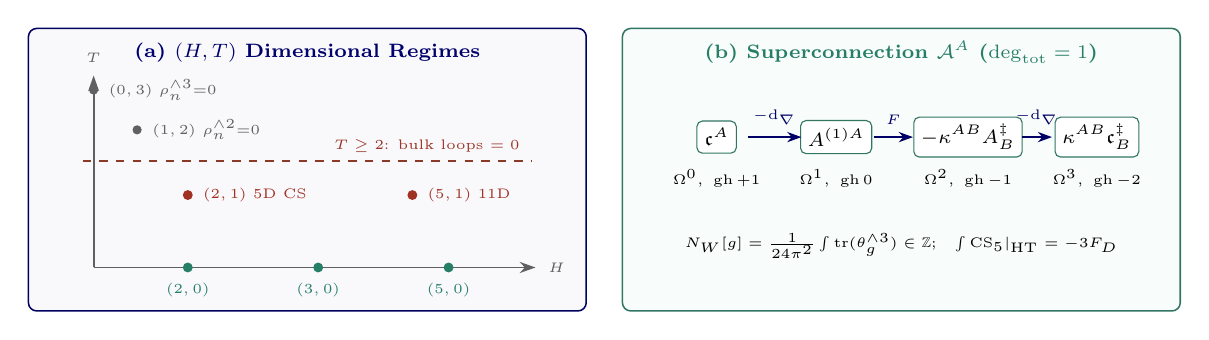
\begin{tikzpicture}[scale=0.92]
  % Left: Dimensional ladder on R^T x C^H
  \begin{scope}[shift={(-4.10,0)}]
    \draw[rounded corners=3pt, draw=NavyBlue!75!black, fill=NavyBlue!2.5, line width=0.55pt] (-3.85,-1.95) rectangle (3.85,1.95);
    \node[font=\scriptsize\bfseries, text=NavyBlue!85!black] at (0,1.62) {(a) $(H,T)$ Dimensional Regimes};
    \draw[-{Stealth[length=2.0mm,width=1.4mm]}, line width=0.7pt, gray!75!black] (-2.95,-1.35) -- (-2.95,1.30) node[above=1pt, font=\tiny] {$T$};
    \draw[-{Stealth[length=2.0mm,width=1.4mm]}, line width=0.7pt, gray!75!black] (-2.95,-1.35) -- ( 3.15,-1.35) node[right=1pt, font=\tiny] {$H$};
    \filldraw[PineGreen!85!black] (-1.65,-1.35) circle (0.06cm) node[below=2pt, font=\tiny] {$(2,0)$};
    \filldraw[PineGreen!85!black] ( 0.15,-1.35) circle (0.06cm) node[below=2pt, font=\tiny] {$(3,0)$};
    \filldraw[PineGreen!85!black] ( 1.95,-1.35) circle (0.06cm) node[below=2pt, font=\tiny] {$(5,0)$};
    \filldraw[BrickRed!85!black]  (-1.65,-0.35) circle (0.06cm) node[right=2pt, font=\tiny] {$(2,1)$ $5\mathrm{D}$ CS};
    \filldraw[BrickRed!85!black]  ( 1.45,-0.35) circle (0.06cm) node[right=2pt, font=\tiny] {$(5,1)$ $11\mathrm{D}$};
    \filldraw[gray!75!black]      (-2.35, 0.55) circle (0.055cm) node[right=2pt, font=\tiny] {$(1,2)$ $\rho_n^{\wedge 2}{=}0$};
    \filldraw[gray!75!black]      (-2.95, 1.10) circle (0.055cm) node[right=2pt, font=\tiny] {$(0,3)$ $\rho_n^{\wedge 3}{=}0$};
    \draw[dashed, BrickRed!70!black, line width=0.5pt] (-3.10,0.12) -- (3.10,0.12);
    \node[font=\tiny, text=BrickRed!80!black] at (1.65,0.32) {$T \ge 2$: bulk loops $= 0$};
  \end{scope}

  % Right: AKSZ superconnection form-degree triangle
  \begin{scope}[shift={(4.10,0)}]
    \draw[rounded corners=3pt, draw=PineGreen!75!black, fill=PineGreen!2.5, line width=0.55pt] (-3.85,-1.95) rectangle (3.85,1.95);
    \node[font=\scriptsize\bfseries, text=PineGreen!85!black] at (0,1.62) {(b) Superconnection $\mathcal{A}^A$ ($\deg_{\mathrm{tot}}=1$)};
    \foreach \xx/\yy/\lbl/\sub in {
      -2.55/ 0.45/{\ghc^A}/{$\Omega^0,\ \mathrm{gh}\,{+}1$},
      -0.90/ 0.45/{A^{(1)A}}/{$\Omega^1,\ \mathrm{gh}\,0$},
       0.92/ 0.45/{-\kappa^{AB}A^\ddagger_B}/{$\Omega^2,\ \mathrm{gh}\,{-}1$},
       2.70/ 0.45/{\kappa^{AB}\ghc^\ddagger_B}/{$\Omega^3,\ \mathrm{gh}\,{-}2$}%
    } {
      \node[draw=PineGreen!75!black, rounded corners=2pt, fill=white, inner sep=2.6pt, font=\scriptsize] at (\xx,0.45) {$\lbl$};
      \node[font=\tiny] at (\xx,-0.12) {\sub};
    }
    \draw[-{Stealth[length=1.8mm,width=1.3mm]}, line width=0.6pt, NavyBlue!80!black] (-2.12,0.45) -- node[above=1pt, font=\tiny] {$-\dd_\nabla$} (-1.38,0.45);
    \draw[-{Stealth[length=1.8mm,width=1.3mm]}, line width=0.6pt, NavyBlue!80!black] (-0.38,0.45) -- node[above=1pt, font=\tiny] {$F$} ( 0.16,0.45);
    \draw[-{Stealth[length=1.8mm,width=1.3mm]}, line width=0.6pt, NavyBlue!80!black] ( 1.66,0.45) -- node[above=1pt, font=\tiny] {$-\dd_\nabla$} ( 2.08,0.45);
    \node[font=\tiny] at (0,-1.05) {$N_W[g] = \frac{1}{24\pi^2}\int\tr(\theta_g^{\wedge 3})\in\ZZ$;\quad $\int\mathrm{CS}_5|_{\mathrm{HT}} = -3F_D$};
  \end{scope}
\end{tikzpicture}
\caption{Visual dictionary for Background Card~6.1 and Propositions~\ref{prop:cs3-large-gauge-nw}--\ref{prop:bv-aksz-cs}: (a)~phase diagram of $(H,T)$ field theories showing pure holomorphic ($T=0$) and critical HT ($T=1$) regimes below the $T \ge 2$ Pfaffian vanishing line $\rho_n(M)^{\wedge T} = 0$; (b)~AKSZ superconnection tower~\eqref{eq:aksz-superconnection} with right-placed antifields, integer winding $N_W[g]\in\ZZ$, and $-3F_D$ restriction.}
\label{fig:cs-aksz-ladder}
\end{figure}

\subsection{Commutative \texorpdfstring{$5\mathrm{D}$}{5D} Chern--Simons Diagrams, In-Situ Whitehead--Vogel Color Ladders, and All-Order Quantization}
\label{subsec:5d-cs-flagship}

On $X = \RR_\tau\times\C^2_z$ ($H=2, T=1, D=3$, $\Omega = \dd z^1\wedge\dd z^2$; companion paper~\fivedpdf), commutative $5\mathrm{D}$ Chern--Simons has $\mathcal{A}^A \in \Omega^\bullet(\RR_\tau)\widehat{\otimes}\Omega^{0,\bullet}(\C^2)\otimes\fg[1]$ and $S_{E,\mathrm{cl}}[\mathcal{A}] = \int_{\RR\times\C^2}\Omega\wedge(\frac{1}{2}\kappa_{AB}\mathcal{A}^A D_{\mathrm{free}}\mathcal{A}^B + \frac{1}{6}f_{ABC}\mathcal{A}^A\mathcal{A}^B\mathcal{A}^C)$. We first isolate the holomorphic--topological local complex and compute the spacetime integrals of the two-loop Feynman diagrams, and then introduce the Lie--Whitehead and Vogel split-Casimir background cards right at the step where the diagram color factors must be contracted and classified.

\begin{lemma}[{$8$-summand Koszul decomposition $V \cong \bigoplus_{S\subset\{1,2,3\}}V_S$ vs.\ $\eta_v$-contraction projection~{\cite{WW24,Repo9e833c8}}}]
\label{lem:5d-cs-8summands}
Let $V := \mathrm{Loc}_{\mathrm{trans}}(\mathcal{E})$ denote the cochain complex of translation-invariant local functionals of $\mathcal{A}^A \in \Omega^\bullet(\RR_\tau)\widehat{\otimes}\Omega^{0,\bullet}(\C^2_z)\otimes\fg[1]$ under $Q_0 = \{S_{E,\mathrm{cl}}, -\}$.
\begin{enumerate}[label=(\arabic*),leftmargin=*]
  \item Expanding polyform densities in the constant basis $(e_1,e_2,e_3) := (\dd\tau, \dd\bar{z}^{\bar{1}}, \dd\bar{z}^{\bar{2}})$ splits $V = \bigoplus_{\substack{S\subseteq\{1,2,3\}\\\mathrm{form\ subsets}}}V_S$ into $2^3 = 8$ $Q_0$-closed summands, containing non-holomorphic ghost-$0$ cohomology classes such as $G_\eps = \int_{\RR\times\C^2}\dd\tau\wedge\dd z^1\wedge\dd z^2\wedge\dd\bar{z}^{\bar{1}}\,\kappa_{AB}\mathcal{A}^A\partial_\tau\mathcal{A}^B$ and $T_\lambda = \int_{\RR\times\C^2}\dd z^1\wedge\dd z^2\wedge\dd\bar{z}^{\bar{1}}\wedge\dd\bar{z}^{\bar{2}}\,f_{ABC}\mathcal{A}^A\mathcal{A}^B\partial_\tau\mathcal{A}^C$ outside the top $(\dd\tau\wedge\dd\bar{z}^{\bar{1}}\wedge\dd\bar{z}^{\bar{2}})$-sector.

  \item Imposing odd interior-contraction invariance $\eta_v F = 0$ for all $v \in \{\partial_\tau, \partial_{\bar{z}^{\bar{1}}}, \partial_{\bar{z}^{\bar{2}}}\}$ (automatic for $S_{E,\mathrm{cl}}$ and every Costello heat-kernel Feynman graph built from $D_{\mathrm{free}}$-invariant vertices and $D^* K_t$) kills the $7$ lower summands $S \subsetneq \{1,2,3\}$ and identifies the surviving holomorphic--topological subcomplex $V_{\mathrm{ht}} := V_{\{1,2,3\}}$ quasi-isomorphically with shifted balanced current cochains:
  \begin{equation}
  \label{eq:5d-vht-iso}
  H^g(V_{\mathrm{ht}}, Q_0) \cong H^{g+3}\!\bigl((C^0_{\fg[[z^1,z^2]]})^G,\, d_{\mathrm{CE}}\bigr).
  \end{equation}
\end{enumerate}
\end{lemma}

\begin{proof}\leavevmode
\begin{proofpart}{Claim 1: Decoupling of $D_{\mathrm{free}}$ on translation-invariant jets}
On translation-invariant local functionals, integration by parts identifies total derivatives $\partial_\tau(\cdots) = \dbar_{\bar{\jmath}}(\cdots) = 0$, annihilating the kinetic operator $D_{\mathrm{free}} = \dd\tau\partial_\tau + \dd\bar{z}^{\bar{\jmath}}\dbar_{\bar{\jmath}}$ inside $Q_0$ and reducing $Q_0$ purely to the $\fg[[z^1,z^2,\tau,\bar{z}]]$-jet Chevalley--Eilenberg differential preserving each exterior subset $S \subseteq \{1,2,3\}$. Direct cocycle evaluation confirms $Q_0 G_\eps = Q_0 T_\lambda = 0$ with $G_\eps \in V_{\{1,2\}}$ and $T_\lambda \in V_{\{2,3\}}$.
\end{proofpart}
\begin{proofpart}{Claim 2: Interior contraction projection and $(\tau,\bar{z})$-Poincar\'e retraction}
On $\mathcal{A} = \sum_{\substack{I\subseteq\{1,2,3\}\\\mathrm{components}}}e_I\mathcal{A}_I$, the derivation $\eta_{\partial_{a}}$ acts as $\partial/\partial e_a$ on explicit $1$-forms, so $\bigcap_{\substack{a\in\{1,2,3\}\\\mathrm{dirs}}}\ker\eta_{\partial_a} = V_{\{1,2,3\}}$ consists precisely of full-wedge functionals $\int\Omega\wedge\dd\tau\wedge\dd\bar{z}^{\bar{1}}\wedge\dd\bar{z}^{\bar{2}}\,\mathcal{L}(\mathcal{A},\partial_z^\alpha\mathcal{A})$ evaluated on the superfield $\mathcal{A}$ without explicit $(\partial_\tau,\partial_{\bar{z}})$ jet insertions, shifting ghost degree by $+3$ to yield~\eqref{eq:5d-vht-iso}.
\end{proofpart}
\end{proof}

\paragraph{Spacetime evaluation of the two-loop $5\mathrm{D}$ Chern--Simons Feynman diagrams before color contraction.}
Because $T = 1$, odd loop orders vanish ($O_{2m+1} = 0$). At two loops ($n = 2, D = 3, |I| = 7, |V| = 6$, $E_{\mathrm{ext}} = 4$ external gauge legs), $3$-Laman admissibility~\eqref{eq:d-laman-inequalities} admits two tight Feynman topologies: $\theta(1,3,3)$ and $\theta(2,2,3)$ (Figure~\ref{fig:5d-9d-cs}(a)). In Worked Example~\ref{ex:pareto-and-5d-theta}, Theorem~\ref{thm:theta-closed} evaluated their exact spacetime Schwinger integrals to $K_{133} = -\frac{\pi}{20}[p^{(1)}p^{(2)}][p^{(3)}p^{(4)}]$ and $K_{223} = +\frac{\pi}{30}[p^{(1)}p^{(2)}][p^{(3)}p^{(4)}]$. Dressing the six trivalent vertices with $f_{ABC}$ and the seven propagators with $\kappa^{EF}$ assembles the two-loop QME obstruction $[O_2] = -\frac{U\hbar^2}{3072\pi^4}[F_{223}]$ ($U \in \{\pm 1\}$) inside $H^4((C^0_{\fg[[z^1,z^2]]})^G)$. Determining (a)~for which Lie algebras $[F_{223}]$ vanishes modulo coboundaries $d_{\mathrm{CE}}([q^{(0)}q^{(1)}]^2 f_{ABC})$ and (b)~for which Lie algebras an order-$\hbar$ counterterm $J_1$ can cancel $[O_2]$ now requires two Lie-algebraic tools, which we present in situ as Background Cards~6.2 and~6.3.

\begin{figure}[H]
\centering
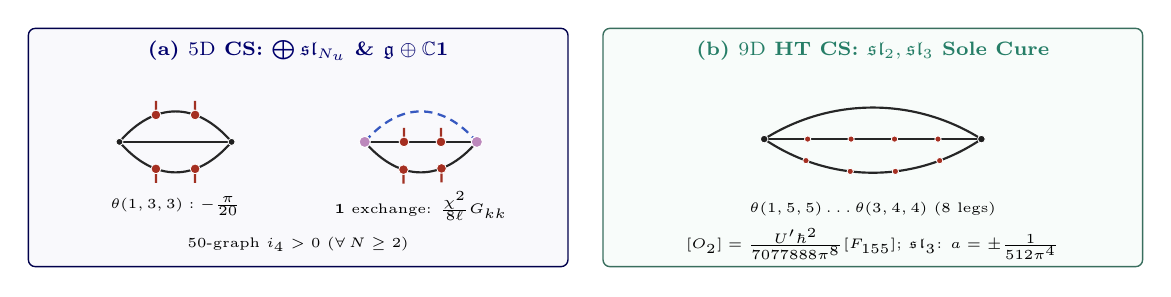
\begin{tikzpicture}[scale=0.89]
  % Left: 5D CS theta + central exchange
  \begin{scope}[shift={(-4.10,0)}]
    \draw[rounded corners=2.5pt, draw=NavyBlue!60!black, fill=NavyBlue!2.5, line width=0.5pt] (-3.85,-1.70) rectangle (3.85,1.70);
    \node[font=\scriptsize\bfseries, text=NavyBlue!85!black] at (0,1.38) {(a) $5\mathrm{D}$ CS: $\bigoplus\fsl_{N_u}$ \& $\fg\oplus\C\mathbf{1}$};
    \begin{scope}[shift={(-1.75,0.08)}]
      \coordinate (l) at (-0.80,0); \coordinate (r) at (0.80,0);
      \draw[prop] (l) .. controls (-0.30,0.58) and (0.30,0.58) .. node[pos=0.33, vbiv, scale=0.8] (a1) {} node[pos=0.67, vbiv, scale=0.8] (a2) {} (r);
      \draw[prop] (l)--(r);
      \draw[prop] (l) .. controls (-0.30,-0.58) and (0.30,-0.58) .. node[pos=0.33, vbiv, scale=0.8] (b1) {} node[pos=0.67, vbiv, scale=0.8] (b2) {} (r);
      \draw[extleg] (a1)--++(0,0.20); \draw[extleg] (a2)--++(0,0.20);
      \draw[extleg] (b1)--++(0,-0.20); \draw[extleg] (b2)--++(0,-0.20);
      \filldraw[v0] (l) circle (0.05cm); \filldraw[v0] (r) circle (0.05cm);
      \node[font=\tiny] at (0,-0.92) {$\theta(1,3,3): -\frac{\pi}{20}$};
    \end{scope}
    \begin{scope}[shift={(1.75,0.08)}]
      \coordinate (xl) at (-0.80,0); \coordinate (xr) at (0.80,0);
      \draw[cprop] (xl) .. controls (-0.30,0.58) and (0.30,0.58) .. (xr);
      \draw[prop] (xl) -- node[pos=0.35, vbiv, scale=0.8] (xa) {} node[pos=0.68, vbiv, scale=0.8] (xb) {} (xr);
      \draw[prop] (xl) .. controls (-0.30,-0.58) and (0.30,-0.58) .. node[pos=0.35, vbiv, scale=0.8] (xc) {} node[pos=0.68, vbiv, scale=0.8] (xd) {} (xr);
      \draw[extleg] (xa)--++(0,0.20); \draw[extleg] (xb)--++(0,0.20);
      \draw[extleg] (xc)--++(0,-0.20); \draw[extleg] (xd)--++(0,-0.20);
      \node[vtcent, scale=0.82] at (xl) {}; \node[vtcent, scale=0.82] at (xr) {};
      \node[font=\tiny] at (0,-0.92) {$\mathbf{1}$ exchange: $\frac{\chi^2}{8\ell}G_{kk}$};
    \end{scope}
    \node[font=\tiny] at (0,-1.38) {$50$-graph $i_4 > 0$ ($\forall\,N\ge 2$)};
  \end{scope}

  % Right: 9D CS theta(1,5,5)..theta(3,4,4) -> sl_2, sl_3
  \begin{scope}[shift={(4.10,0)}]
    \draw[rounded corners=2.5pt, draw=PineGreen!65!black, fill=PineGreen!2.5, line width=0.5pt] (-3.85,-1.70) rectangle (3.85,1.70);
    \node[font=\scriptsize\bfseries, text=PineGreen!85!black] at (0,1.38) {(b) $9\mathrm{D}$ HT CS: $\fsl_2, \fsl_3$ Sole Cure};
    \coordinate (nl) at (-1.55,0.12); \coordinate (nr) at (1.55,0.12);
    \draw[prop] (nl) .. controls (-0.60,0.72) and (0.60,0.72) .. (nr);
    \draw[prop] (nl)--(nr);
    \draw[prop] (nl) .. controls (-0.60,-0.52) and (0.60,-0.52) .. (nr);
    \foreach \tt in {0.2,0.4,0.6,0.8} {
      \path (nl) -- coordinate[pos=\tt] (pm) (nr); \filldraw[vbiv] (pm) circle (0.045cm);
      \path (nl) .. controls (-0.60,-0.52) and (0.60,-0.52) .. coordinate[pos=\tt] (pd) (nr); \filldraw[vbiv] (pd) circle (0.045cm);
    }
    \filldraw[v0] (nl) circle (0.054cm); \filldraw[v0] (nr) circle (0.054cm);
    \node[font=\tiny] at (0,-0.88) {$\theta(1,5,5)\dots\theta(3,4,4)$ ($8$ legs)};
    \node[font=\tiny] at (0,-1.38) {$[O_2] = \frac{U'\hbar^2}{7077888\pi^8}[F_{155}]$;\ $\fsl_3$: $a = \pm\frac{1}{512\pi^4}$};
  \end{scope}
\end{tikzpicture}
\caption{Two-loop Chern--Simons Feynman diagrams whose color contractions motivate Background Cards~6.2--6.3 (Theorems~\ref{thm:5d-cs-allorders} and~\ref{thm:9d-10d-cs}): (a)~$5\mathrm{D}$ CS $4$-leg theta topologies $\theta(1,3,3), \theta(2,2,3)$, central $\mathbf{1}$ exchange, and $50$-graph $\hbar^4$ lift; (b)~$9\mathrm{D}$ CS $8$-leg theta topologies $\theta(1,5,5)\dots\theta(3,4,4)$ leaving $\fsl_2, \fsl_3$ as the sole simple solutions.}
\label{fig:5d-9d-cs}
\end{figure}

\phantomsection\label{subsec:lie-whitehead}
\begin{zkmodule}{Chevalley Casimirs, $\fg$-Invariants vs.\ $\Hom_{\fg}$, Whitehead's Theorem, and Cubic Tensors}{low-rank-isomorphisms-cubic-invariants}
Let $\fg$ be a finite-dimensional complex simple Lie algebra of dimension $d_{\fg} = \dim_{\C}\fg$ and rank $r_{\fg} = \dim_{\C}\fh$, with root decomposition $\fg = \fh \oplus \bigoplus_{\substack{\alpha\in\Phi\\\mathrm{roots}}}\fg_\alpha$, Killing form $\kappa^{\mathrm{Kill}}_{AB} := \Tr_{\fg}(\ad(T_A)\ad(T_B)) = 2h^\vee\kappa^{\mathrm{norm}}_{AB}$ (dual Coxeter number $h^\vee$), and Weyl group $W$.

\paragraph{1.\ What the Chevalley generators $(P_1,\dots,P_{r_{\fg}})$ mean.}
An element $P \in \Sym^d(\fg^*)$ is a degree-$d$ homogeneous polynomial on $\fg$; it is $\ad$-invariant ($P \in \Sym^d(\fg^*)^{\fg}$) when $P([Z,X],\dots,X) = 0$ for all $X,Z \in \fg$, corresponding under PBW symmetrization to a central Casimir operator in $Z(U(\fg))$. \emph{Chevalley's restriction theorem} states that restricting polynomials from $\fg$ to $\fh$ induces a graded algebra isomorphism $\Sym(\fg^*)^{\fg} \xrightarrow{\cong} \Sym(\fh^*)^W \cong \C[P_1,\dots,P_{r_{\fg}}]$, generated by $r_{\fg}$ algebraically independent homogeneous \emph{primitive Casimir generators} $P_1,\dots,P_{r_{\fg}}$ of degrees $d_1 \le \dots \le d_{r_{\fg}}$ ($\sum_{\substack{s\in\{1,\dots,r_{\fg}\}\\\mathrm{generators}}}(2d_s - 1) = d_{\fg}$):
\begin{itemize}[leftmargin=*]
  \item $A_{N-1} = \fsl_N(\C)$ ($r_{\fg} = N-1$): degrees $2, 3, 4, \dots, N$, realized by matrix power traces $P_{k-1}(X) = \tr_{\C^N}(X^k)$ ($k=2,\dots,N$). Crucially, \emph{$\fsl_N$ with $N \ge 3$ is the sole simple family possessing a degree-$3$ generator $P_2(X) = \tr(X^3)$!}
  \item $B_r = \fso_{2r+1}$ and $C_r = \fsp_{2r}$: purely even degrees $2, 4, \dots, 2r$ (since $-\mathbf{1} \in W$ kills all odd-$d$ Weyl invariants).
  \item $D_r = \fso_{2r}$ ($r \ge 3$): degrees $2, 4, \dots, 2r-2$ plus the degree-$r$ Pfaffian $\Pf(X)$ (giving a second quartic at $D_4 = \fso_8$, where $\Spin(8)$ triality permutes $8_v, 8_s, 8_c$, and a quintic Pfaffian at $D_5 = \fso_{10}$, while $D_3 \cong A_3$ recovers $\fso_6 \cong \fsl_4$, alongside $A_1 \cong B_1 \cong C_1$, $B_2 \cong C_2$, and $D_2 \cong \fsl_2\oplus\fsl_2$).
  \item Exceptionals $G_2$ ($2,6$), $F_4$ ($2,6,8,12$), $E_6$ ($2,5,6,8,9,12$), $E_7$ ($2,6,8,10,12,14,18$), $E_8$ ($2,8,12,14,18,20,24,30$): zero degree-$3$ generators ($E_6$ has a quintic $\tr_{\mathbf{27}}(X^5)$ tested in $9\mathrm{D}$ CS).
\end{itemize}

\paragraph{2.\ Meaning of $\fg$-invariants $V^{\fg}$ and $\fg$-equivariant maps $\Hom_{\fg}(V,W)$.}
For $\fg$-representations $(V,\rho_V)$ and $(W,\rho_W)$:
\begin{equation}
\label{eq:Vg-and-Homg-def}
\begin{aligned}
V^{\fg} &:= \bigl\{v \in V : \rho_V(Z)v = 0\ \ \forall\,Z\in\fg\bigr\},\\
\Hom_{\fg}(V,W) &:= \bigl\{\Phi \in \Hom_{\C}(V,W) : \rho_W(Z)\circ\Phi = \Phi\circ\rho_V(Z)\ \ \forall\,Z\in\fg\bigr\}.
\end{aligned}
\end{equation}
Via $(V^*\otimes W)^{\fg} \cong \Hom_{\fg}(V,W)$ and Killing self-duality $\fg \cong \fg^*$, trilinear invariant tensors split as $(\fg^{*\otimes 3})^{\fg} \cong \Hom_{\fg}(\fg\otimes\fg, \fg) \cong \Hom_{\fg}(\Lambda^2\fg, \fg) \oplus \Hom_{\fg}(\Sym^2\fg, \fg)$.
\end{zkmodule}

\begin{proposition}[Whitehead's lemmas, $H^3(\fg;\C) \cong \C$, and uniqueness of $f_{ABC}$ and $d_{ABC}$]
\label{prop:whitehead-cubic-proof}
For every finite-dimensional complex simple Lie algebra $\fg$:
\begin{enumerate}[label=(\alph*),leftmargin=*]
  \item $H^1(\fg;V) = H^2(\fg;V) = 0$ for every finite-dimensional $\fg$-module $V$, and $H^\bullet(\fg;\C) \cong (\Lambda^\bullet\fg^*)^{\fg}$;
  \item $H^3(\fg;\C) \cong (\Lambda^3\fg^*)^{\fg} = \C\cdot f_{ABC}$ is $1$-dimensional, so $\dim\Hom_{\fg}(\Lambda^2\fg,\fg) = 1$ (spanned by $[\cdot,\cdot]$);
  \item $\dim(\Sym^3\fg^*)^{\fg} = 1$ for $\fg \cong \fsl_N$ ($N \ge 3$, spanned by $d_{ABC} := \frac{1}{2}\tr_{\C^N}(T_A\{T_B,T_C\})$) and $0$ for every other simple $\fg$.
\end{enumerate}
\end{proposition}

\begin{proof}\leavevmode
\begin{proofpart}{Part (a): Casimir homotopy proof of Whitehead's lemmas}
By Weyl complete reducibility, reduce to irreducible $V$. When $V = \C$, $d_{\mathrm{CE}}\alpha(X,Y) = -\alpha([X,Y])$ vanishes on $[\fg,\fg] = \fg$, so $H^1(\fg;\C) = 0$. When $V \neq \C$ is nontrivial irreducible, the quadratic Casimir $C_2^V := \kappa^{AB}\rho_V(T_A)\rho_V(T_B) \in \End_{\fg}(V)$ acts by a nonzero scalar $c_V \neq 0$ (trace check via Weyl's dimension formula). Defining the degree-$(-1)$ contracting homotopy $h : C^p(\fg;V) \to C^{p-1}(\fg;V)$ by $(h\omega)(X_1,\dots,X_{p-1}) := \kappa^{AB}\rho_V(T_A)\,\omega(T_B, X_1,\dots,X_{p-1})$, standard Cartan calculus $[d_{\mathrm{CE}},\iota_Z] + \iota_Z d_{\mathrm{CE}} = \mathcal{L}_Z$ gives $(d_{\mathrm{CE}}h + h d_{\mathrm{CE}})\omega = C_2^V\omega = c_V\omega$, proving $H^p(\fg;V) = 0$ for all $p \ge 0$ on nontrivial irreducible $V$, and leaving $H^p(\fg;\C) \cong (\Lambda^p\fg^*)^{\fg}$ because $\mathcal{L}_Z = \iota_Z d_{\mathrm{CE}} + d_{\mathrm{CE}}\iota_Z$ vanishes on $(\Lambda^\bullet\fg^*)^{\fg}$. At $p=2$, any $\omega \in (\Lambda^2\fg^*)^{\fg}$ defines $J \in \Hom_{\fg}(\fg,\fg)$ via $\omega(X,Y) = \kappa(JX,Y)$; Schur's lemma forces $J = c\,\id_{\fg}$, hence $\omega(-,-) = -\omega(-,-) = 0$ and $H^2(\fg;\C) = 0$.
\end{proofpart}
\begin{proofpart}{Part (b): One-dimensionality of $(\Lambda^3\fg^*)^{\fg}$ and $\Hom_{\fg}(\Lambda^2\fg,\fg)$}
First, $f_{ABC} = \kappa(T_A,[T_B,T_C])$ is totally skew and $d_{\mathrm{CE}}$-closed by Jacobi, with $f_{ABC}\kappa^{AE}f^E{}_{BF} = -\kappa^{\mathrm{Kill}}_{CF} \neq 0$, so $\dim(\Lambda^3\fg^*)^{\fg} \ge 1$. Conversely, any $\omega \in (\Lambda^3\fg^*)^{\fg}$ defines an intertwiner $\Phi \in \Hom_{\fg}(\Lambda^2\fg,\fg)$ via $\kappa(X,\Phi(Y\wedge Z)) = \omega(X,Y,Z)$. On the highest-root vector $E_\theta \in \fg_\theta$, weight conservation maps $\Lambda^2\fg$ onto $\fg_\theta$ via root pairs $\alpha + \beta = \theta$, fixing $\Phi$ up to a single scalar multiple of $[\cdot,\cdot]$ by simplicity of $\fg$ (equivalently via Hopf's theorem $H^\bullet(G;\C) \cong \Lambda^\bullet(x_{2d_1-1},\dots,x_{2d_{r_{\fg}}-1})$ with unique degree-$3$ generator $x_3$ from $d_1 = 2$).
\end{proofpart}
\begin{proofpart}{Part (c): Symmetric cubic invariants}
Polarizing degree-$3$ polynomials in $\Sym(\fg^*)^{\fg} \cong \C[P_1,\dots,P_{r_{\fg}}]$ shows $\dim(\Sym^3\fg^*)^{\fg}$ counts primitive generators of degree $d_s = 3$, which equals $1$ for $A_{N-1}$ ($N \ge 3$) and $0$ for $A_1, B_r, C_r, D_r, G_2, F_4, E_{6,7,8}$.
\end{proofpart}
\end{proof}

\begin{example}[Explicit cubic check on $\fsl_2$ vs.\ $\fsl_3$]
\label{ex:sl2-sl3-cubic}
For $X \in \fsl_2(\C)$ ($\tr X = 0$), Cayley--Hamilton $X^2 - \frac{1}{2}(\tr X^2)\mathbf{1}_2 = 0$ multiplies by $X$ and traces to give $\tr(X^3) = \frac{1}{2}(\tr X^2)(\tr X) = 0$ identically, confirming $(\Sym^3\fsl_2^*)^{\fsl_2} = 0$. For $X = \diag(1,1,-2) \in \fsl_3(\C)$, $\tr(X^3) = 1 + 1 - 8 = -6 \neq 0$, witnessing $d_{ABC} \neq 0$.
\end{example}

\phantomsection\label{subsec:vogel-plane}
\begin{zkmodule}{Split Casimir Ladders $m_k, n_k$, Semisimple vs.\ Simple $X_2$, and Vogel's Plane}{vogel-universal-plane}
To contract the six structure constants $f_{ABC}$ inside the two-loop $5\mathrm{D}$ Chern--Simons theta graphs $\theta(1,3,3)$ and $\theta(2,2,3)$ uniformly across all Lie types, note that those contractions form two parallel adjoint lines joined by $k = 4$ Killing-inverse rungs $(\kappa^{\mathrm{Kill},-1})^{FG}$. For any representations $(V,\rho_V)$ and $(W,\rho_W)$ of a Lie algebra $\fg$ equipped with nondegenerate $\ad$-invariant symmetric form $\kappa_{AB}$ (inverse $\kappa^{AB}$), define the quadratic Casimir $C_2(V) := \kappa^{AB}\rho_V(T_A)\rho_V(T_B)$ and \emph{split Casimir operator} $\Omega_{V\otimes W} := \kappa^{AB}\rho_V(T_A)\otimes\rho_W(T_B) \in \End_{\fg}(V\otimes W)$. On $V = W = \fg_{\mathrm{ad}}$ in Killing normalization $\kappa = \kappa^{\mathrm{Kill}}$, set $\Omega_{\mathrm{ad}} := \Omega_{\fg\otimes\fg}$ and tensor-flip $P_{\mathrm{ex}}(X\otimes Y) := Y\otimes X$, with planar and M\"obius ladder traces (Figure~\ref{fig:split-casimir-vogel}):
\begin{equation}
\label{eq:mk-nk-traces}
m_k := \Tr_{\fg\otimes\fg}\bigl(\Omega_{\mathrm{ad}}^k\bigr),\qquad
n_k := \Tr_{\fg\otimes\fg}\bigl(P_{\mathrm{ex}}\Omega_{\mathrm{ad}}^k\bigr)\qquad (k \in \ZZ_{\ge 1}).
\end{equation}
Decomposing $\fg\otimes\fg = \Lambda^2\fg \oplus \Sym^2\fg$ ($P_{\mathrm{ex}}|_{\Lambda^2\fg} = -1$, $P_{\mathrm{ex}}|_{\Sym^2\fg} = +1$), Proposition~\ref{prop:casimir-x2-semisimple} and Theorem~\ref{thm:vogel-dim-and-8n4} establish the exact hypotheses and eigenvalues on both sectors:
\begin{enumerate}[leftmargin=*]
  \item \emph{Antisymmetric square $\Lambda^2\fg$ (\textbf{valid for every semisimple $\fg$}):} Whenever $\fg$ is \emph{semisimple}, $[\cdot,\cdot] : \Lambda^2\fg \twoheadrightarrow \fg$ is surjective ($[\fg,\fg] = \fg$) and splits $\fg$-equivariantly into $\Lambda^2\fg = \fg_{\mathrm{ad}} \oplus X_2$, where $X_2 := \ker([\cdot,\cdot] : \Lambda^2\fg \to \fg)$ has dimension $\dim X_2 = \binom{d_{\fg}}{2} - d_{\fg} = \frac{1}{2}d_{\fg}(d_{\fg} - 3)$ (vanishing among nonzero semisimple $\fg$ precisely for $\fg \cong \fsl_2$), with $\Omega_{\mathrm{ad}}|_{\fg_{\mathrm{ad}}} = -\frac{1}{2}\id_{\fg_{\mathrm{ad}}}$ and $\Omega_{\mathrm{ad}}|_{X_2} = 0$!
  \item \emph{Symmetric square $\Sym^2\fg$ (\textbf{requires $\fg$ to be simple}):} When $\fg$ is \emph{simple} (so $(\Sym^2\fg)^{\fg} = \C\cdot c_{\mathrm{Kill}}$ is $1$-dimensional, whereas semisimple $\fg = \bigoplus_{\substack{u\in\{1,\dots,m\}\\\mathrm{ideals}}}\fg_u$ with $m \ge 2$ has $\dim(\Sym^2\fg)^{\fg} = m$ plus mixed summands $\fg_u\otimes\fg_v$), Vogel and Mkrtchyan--Sergeev--Veselov~\cite{MSV11} decompose $\Sym^2\fg = \C\oplus Y_2(v_1)\oplus Y_2(v_2)\oplus Y_2(v_3)$ in projective \emph{Vogel parameters} $(v_1 : v_2 : v_3) \in \mathbb{CP}^2/S_3$ ($t_V := v_1 + v_2 + v_3 \neq 0$, $C_2^{\mathrm{Kill}}|_{Y_2(v_s)} = (2 - \frac{v_s}{t_V})\id$):
  \begin{equation}
  \label{eq:vogel-dim-and-eigen}
  d_{\fg} = \frac{(v_1 - 2t_V)(v_2 - 2t_V)(v_3 - 2t_V)}{v_1 v_2 v_3},\qquad
  \Omega_{\mathrm{ad}}\big|_{\C} = -1,\qquad
  \Omega_{\mathrm{ad}}\big|_{Y_2(v_s)} = -\frac{v_s}{2t_V}\,\id.
  \end{equation}
\end{enumerate}
\end{zkmodule}

\begin{figure}[H]
\centering
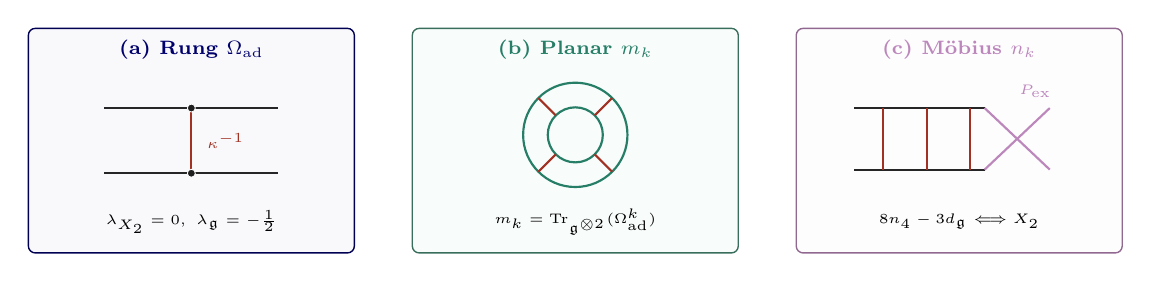
\begin{tikzpicture}[scale=0.92]
  % 1-rung Omega_ad
  \begin{scope}[shift={(-5.30,0)}]
    \draw[rounded corners=2.5pt, draw=NavyBlue!65!black, fill=NavyBlue!2.5, line width=0.5pt] (-2.25,-1.55) rectangle (2.25,1.55);
    \node[font=\scriptsize\bfseries, text=NavyBlue!85!black] at (0,1.25) {(a) Rung $\Omega_{\mathrm{ad}}$};
    \draw[prop] (-1.20,0.45) -- (1.20,0.45);
    \draw[prop] (-1.20,-0.45) -- (1.20,-0.45);
    \draw[prop, BrickRed!85!black] (0,0.45) -- node[right=2pt, font=\tiny, text=BrickRed!85!black] {$\kappa^{-1}$} (0,-0.45);
    \filldraw[v0] (0,0.45) circle (0.055cm);
    \filldraw[v0] (0,-0.45) circle (0.055cm);
    \node[font=\tiny] at (0,-1.12) {$\lambda_{X_2}=0,\ \lambda_{\fg}=-\frac{1}{2}$};
  \end{scope}

  % Planar ladder m_k
  \begin{scope}[shift={(0,0)}]
    \draw[rounded corners=2.5pt, draw=PineGreen!65!black, fill=PineGreen!2.5, line width=0.5pt] (-2.25,-1.55) rectangle (2.25,1.55);
    \node[font=\scriptsize\bfseries, text=PineGreen!85!black] at (0,1.25) {(b) Planar $m_k$};
    \draw[prop, PineGreen!85!black] (0,0.08) circle (0.72cm);
    \draw[prop, PineGreen!85!black] (0,0.08) circle (0.38cm);
    \foreach \ang in {45,135,225,315} {
      \draw[prop, BrickRed!85!black] ($(0,0.08)+({\ang}:0.38cm)$) -- ($(0,0.08)+({\ang}:0.72cm)$);
    }
    \node[font=\tiny] at (0,-1.12) {$m_k = \Tr_{\fg^{\otimes 2}}(\Omega_{\mathrm{ad}}^k)$};
  \end{scope}

  % Moebius ladder n_k
  \begin{scope}[shift={(5.30,0)}]
    \draw[rounded corners=2.5pt, draw=Plum!65!black, fill=Plum!2.5, line width=0.5pt] (-2.25,-1.55) rectangle (2.25,1.55);
    \node[font=\scriptsize\bfseries, text=Plum!85!black] at (0,1.25) {(c) M\"obius $n_k$};
    \draw[prop] (-1.45,0.45) -- (0.35,0.45);
    \draw[prop] (-1.45,-0.40) -- (0.35,-0.40);
    \draw[prop, Plum!85!black] (0.35,0.45) -- (1.25,-0.40);
    \draw[prop, Plum!85!black] (0.35,-0.40) -- (1.25,0.45);
    \foreach \xx in {-1.05,-0.45,0.15} \draw[prop, BrickRed!85!black] (\xx,0.45) -- (\xx,-0.40);
    \node[font=\tiny, text=Plum!85!black] at (1.05,0.68) {$P_{\mathrm{ex}}$};
    \node[font=\tiny] at (0,-1.12) {$8n_4 - 3d_{\fg} \Longleftrightarrow X_2$};
  \end{scope}
\end{tikzpicture}
\caption{Split Casimir ladder operators of Background Card~6.3: (a)~single Killing-inverse rung $\Omega_{\mathrm{ad}}$ annihilating $X_2 = \ker[\cdot,\cdot]$; (b)~planar $k$-rung annulus trace $m_k$; (c)~single-twist M\"obius trace $n_k$ governing the two-loop $5\mathrm{D}$ Chern--Simons color contraction~\eqref{eq:vogel-8n4-proof-eq}.}
\label{fig:split-casimir-vogel}
\end{figure}

\begin{proposition}[{Proof of $C_2(V\otimes W) = C_2(V)\otimes\id + \id\otimes C_2(W) + 2\Omega_{V\otimes W}$, semisimple vs.\ simple hypotheses on $X_2$, and Jacobi vanishing $\Omega_{\mathrm{ad}}|_{X_2} = 0$}]
\label{prop:casimir-x2-semisimple}
\leavevmode
\begin{enumerate}[label=(\arabic*),leftmargin=*]
  \item \emph{Tensor-product Casimir expansion and $C_2^{\mathrm{Kill}}(\fg_{\mathrm{ad}}) = \mathbf{1}_{\fg}$:} For any finite-dimensional Lie algebra $\fg$ with nondegenerate $\ad$-invariant symmetric bilinear form $\kappa_{AB}$ (inverse $\kappa^{AB}$) and any $\fg$-representations $(V,\rho_V), (W,\rho_W)$,
  \begin{equation}
  \label{eq:casimir-tensor-expansion}
  C_2(V\otimes W) = C_2(V)\otimes\id_W + \id_V\otimes C_2(W) + 2\,\Omega_{V\otimes W}.
  \end{equation}
  When $\fg = \bigoplus_{\substack{u\in\{1,\dots,m\}\\\mathrm{simple\ ideals}}}\fg_u$ is complex \textbf{semisimple} in Killing normalization $\kappa = \kappa^{\mathrm{Kill}}$, $C_2^{\mathrm{Kill}}(\fg_{\mathrm{ad}}) = \mathbf{1}_{\fg}$, hence $\Omega_{\mathrm{ad}} = \frac{1}{2}\bigl(C_2^{\mathrm{Kill}}(\fg\otimes\fg) - 2\mathbf{1}_{\fg\otimes\fg}\bigr)$.

  \item \emph{Semisimple sufficiency for $\Lambda^2\fg = \fg_{\mathrm{ad}}\oplus X_2$ vs.\ simple necessity for Vogel's $\Sym^2\fg$:} For \textbf{every semisimple} $\fg$ (whereas non-semisimple reductive algebras with center $\mathfrak{z}(\fg) \neq 0$, such as $\fgl_N = \fsl_N\oplus\C\mathbf{1}$, fail surjectivity $[\fg,\fg]\subsetneq\fg$), $[\cdot,\cdot] : \Lambda^2\fg \twoheadrightarrow \fg$ ($X\wedge Y \mapsto [X,Y]$, $X\wedge Y := X\otimes Y - Y\otimes X$) is surjective with $\fg$-equivariant right inverse $2s : \fg \hookrightarrow \Lambda^2\fg$, $s(Z) := -\frac{1}{2}(\kappa^{\mathrm{Kill},-1})^{AB}[Z,T_A]\wedge T_B$, splitting $\Lambda^2\fg = 2s(\fg)\oplus X_2 \cong \fg_{\mathrm{ad}}\oplus X_2$ with $\dim X_2 = \binom{d_{\fg}}{2} - d_{\fg} = \frac{1}{2}d_{\fg}(d_{\fg}-3)$. Moreover, the Jacobi identity gives on all of $\Lambda^2\fg$
  \begin{equation}
  \label{eq:omega-on-wedge2}
  \Omega_{\mathrm{ad}}(X\wedge Y) = -s\bigl([X,Y]\bigr)
  \quad\Longrightarrow\quad
  \Omega_{\mathrm{ad}}\big|_{\fg_{\mathrm{ad}}} = -\frac{1}{2}\,\id_{\fg_{\mathrm{ad}}},\qquad
  \Omega_{\mathrm{ad}}\big|_{X_2} = 0.
  \end{equation}
  By contrast, Vogel's four-summand decomposition~\eqref{eq:vogel-dim-and-eigen} requires $\fg$ to be \textbf{simple}: for semisimple $\fg = \bigoplus_{\substack{u\in\{1,\dots,m\}\\\mathrm{ideals}}}\fg_u$ with $m \ge 2$, $(\Sym^2\fg)^{\fg} = \bigoplus_{\substack{u\in\{1,\dots,m\}\\\mathrm{ideals}}}(\Sym^2\fg_u)^{\fg_u} \cong \C^m$ has dimension $m \ge 2$ and $\Sym^2\fg$ acquires mixed bi-adjoint summands $\bigoplus_{\substack{1\le u < v \le m\\\mathrm{pairs}}}(\fg_u\otimes\fg_v)$ annihilated by $\Omega_{\mathrm{ad}}$.
\end{enumerate}
\end{proposition}

\begin{proof}\leavevmode
\begin{proofpart}{Part (1): Derivation of $C_2(V\otimes W)$ and Killing normalization $C_2^{\mathrm{Kill}}(\fg_{\mathrm{ad}}) = \mathbf{1}_{\fg}$}
On $V\otimes W$, $\fg$ acts as a derivation $\rho_{V\otimes W}(T_A) := \rho_V(T_A)\otimes\id_W + \id_V\otimes\rho_W(T_A)$. Expanding $C_2(V\otimes W) = \kappa^{AB}\rho_{V\otimes W}(T_A)\rho_{V\otimes W}(T_B)$ gives
\[
\begin{aligned}
C_2(V\otimes W) &= \kappa^{AB}\Bigl(\rho_V(T_A)\rho_V(T_B)\otimes\id_W + \id_V\otimes\rho_W(T_A)\rho_W(T_B)\\
&\qquad\qquad +\; \rho_V(T_A)\otimes\rho_W(T_B) + \rho_V(T_B)\otimes\rho_W(T_A)\Bigr)\\
&= C_2(V)\otimes\id_W + \id_V\otimes C_2(W) + 2\,\Omega_{V\otimes W},
\end{aligned}
\]
where symmetry $\kappa^{BA} = \kappa^{AB}$ relabels $(A\leftrightarrow B)$ in $\kappa^{AB}\rho_V(T_B)\otimes\rho_W(T_A) = \Omega_{V\otimes W}$. For semisimple $\fg = \bigoplus_{\substack{u\in\{1,\dots,m\}\\\mathrm{ideals}}}\fg_u$, $[\fg_u,\fg_v] = 0$ ($u\neq v$) block-diagonalizes $\kappa^{\mathrm{Kill}}_{\fg} = \bigoplus_{\substack{u\in\{1,\dots,m\}\\\mathrm{ideals}}}\kappa^{\mathrm{Kill}}_{\fg_u}$ (nondegenerate by Cartan's criterion). On each simple ideal $\fg_u$, irreducibility of $(\fg_u)_{\mathrm{ad}}$ and Schur's lemma force $C_2^{\mathrm{Kill}}(\fg_u) = \lambda_u\mathbf{1}_{\fg_u}$, and tracing over $\fg_u$ gives $\lambda_u\dim\fg_u = (\kappa_{\fg_u}^{\mathrm{Kill},-1})^{AB}\Tr_{\fg_u}(\ad T_A\ad T_B) = \delta^A{}_A = \dim\fg_u \implies \lambda_u = 1$, hence $C_2^{\mathrm{Kill}}(\fg_{\mathrm{ad}}) = \mathbf{1}_{\fg}$.
\end{proofpart}
\begin{proofpart}{Part (2): Semisimple splitting of $\Lambda^2\fg$ and three-line Jacobi proof of $\Omega_{\mathrm{ad}}|_{X_2} = 0$}
Each simple ideal satisfies $[\fg_u,\fg_u] = \fg_u$, so $[\fg,\fg] = \fg$ for every semisimple $\fg$. Applying $[\cdot,\cdot](U\wedge V) = [U,V]$ to $s(Z) = -\frac{1}{2}(\kappa^{\mathrm{Kill},-1})^{AB}[Z,T_A]\wedge T_B$ gives $[\cdot,\cdot](s(Z)) = -\frac{1}{2}(\kappa^{\mathrm{Kill},-1})^{AB}[[Z,T_A],T_B] = +\frac{1}{2}(\kappa^{\mathrm{Kill},-1})^{AB}\ad(T_B)\ad(T_A)Z = \frac{1}{2}C_2^{\mathrm{Kill}}(\fg_{\mathrm{ad}})(Z) = \frac{1}{2}Z$; thus $[\cdot,\cdot]\circ(2s) = \id_{\fg}$, splitting $\Lambda^2\fg = 2s(\fg)\oplus\ker[\cdot,\cdot] = \fg_{\mathrm{ad}}\oplus X_2$ with $\dim X_2 = \binom{d_{\fg}}{2} - d_{\fg} = \frac{1}{2}d_{\fg}(d_{\fg}-3)$. Next, pairing $\Omega_{\mathrm{ad}}(X\wedge Y) = (\kappa^{\mathrm{Kill},-1})^{EF}([T_E,X]\otimes[T_F,Y] - [T_E,Y]\otimes[T_F,X])$ against $T_G\otimes T_H$ via $\kappa^{\mathrm{Kill}}$ gives $(\kappa^{\mathrm{Kill},-1})^{EF}(f_{GEC}f_{HFD} - f_{GED}f_{HFC})X^C Y^D$. By the Jacobi identity $\kappa^{\mathrm{Kill}}(T_H, [T_G,[T_C,T_D]] + [T_C,[T_D,T_G]] + [T_D,[T_G,T_C]]) = 0$ and total skew-symmetry of $f_{ABC}$, $(\kappa^{\mathrm{Kill},-1})^{EF}(f_{GEC}f_{HFD} - f_{GED}f_{HFC}) = +(\kappa^{\mathrm{Kill},-1})^{EF}f_{EGH}f_{FCD}$, which equals the $(G,H)$ component of $-s([X,Y])$, proving~\eqref{eq:omega-on-wedge2}: $\Omega_{\mathrm{ad}}|_{X_2} = -s\circ[\cdot,\cdot]|_{X_2} = 0$ and $\Omega_{\mathrm{ad}}(2s(Z)) = -s([\cdot,\cdot](2s(Z))) = -s(Z) = -\frac{1}{2}(2s(Z))$. Finally, when $\fg = \fg_1\oplus\fg_2$ has $m \ge 2$ simple ideals, independent Killing forms on $\fg_u$ yield $\dim(\Sym^2\fg)^{\fg} = m \ge 2$ and $\Omega_{\mathrm{ad}}(x_1\otimes x_2) = 0$ on $\fg_1\otimes\fg_2$ since $[\fg_1,\fg_2] = 0$.
\end{proofpart}
\end{proof}

\begin{theorem}[{Proof of Vogel's $\Sym^2\fg$ eigenvalues and dimension formula, universal M\"obius identity $8n_4 - 3d_{\fg}$, and $\fso_{32}$ sextic factorization~{\cite{MSV11,Repo9e833c8}}}]
\label{thm:vogel-dim-and-8n4}
\phantomsection\label{prop:vogel-8n4-identity}\phantomsection\label{lem:vogel-sln-so8}
Let $\fg$ be a finite-dimensional complex \textbf{simple} Lie algebra.
\begin{enumerate}[label=(\arabic*),leftmargin=*]
  \item \emph{Proof of~\eqref{eq:vogel-dim-and-eigen}:} On $\Sym^2\fg = \C\cdot c_{\mathrm{Kill}} \oplus Y_2(v_1)\oplus Y_2(v_2)\oplus Y_2(v_3)$ ($c_{\mathrm{Kill}} := (\kappa^{\mathrm{Kill},-1})^{AB}T_A\otimes T_B$, $C_2^{\mathrm{Kill}}|_{Y_2(v_s)} = (2 - \frac{v_s}{t_V})\id$, $t_V = v_1+v_2+v_3 \neq 0$), Proposition~\ref{prop:casimir-x2-semisimple}(1) gives $\Omega_{\mathrm{ad}}|_{\C} = -1$ and $\Omega_{\mathrm{ad}}|_{Y_2(v_s)} = -\frac{v_s}{2t_V}\id =: \lambda_s\id$ ($\lambda_1+\lambda_2+\lambda_3 = -\frac{1}{2}$), and the trace of the cubic minimal polynomial $\prod_{\substack{s\in\{1,2,3\}\\\mathrm{branches}}}(\Omega_{\mathrm{ad}} - \lambda_s\id)|_{(\Sym^2\fg)_\circ} = 0$ proves $d_{\fg} = \frac{(v_1 - 2t_V)(v_2 - 2t_V)(v_3 - 2t_V)}{v_1 v_2 v_3}$.

  \item \emph{Universal M\"obius trace $8n_4 - 3d_{\fg}$ and Vandermonde branch dimensions:} The four-rung M\"obius trace $n_4 = \Tr_{\fg\otimes\fg}(P_{\mathrm{ex}}\Omega_{\mathrm{ad}}^4)$ obeys
  \begin{equation}
  \label{eq:vogel-8n4-proof-eq}
  8n_4 - 3d_{\fg} = \frac{3\dim(X_2)\,v_1 v_2 v_3}{2t_V^3} = \frac{3d_{\fg}(d_{\fg} - 3)\,v_1 v_2 v_3}{4t_V^3},
  \end{equation}
  vanishing among simple Lie algebras precisely when $\fg \cong \fsl_2$, while the branch dimensions equal $\dim Y_2(v_1) = -\frac{t_V(v_2-2t_V)(v_3-2t_V)(t_V+v_2)(t_V+v_3)(2t_V-3v_1)}{v_1^2 v_2 v_3(v_1-v_2)(v_1-v_3)}$ (and cyclic permutations). In particular, on $\fsl_N(\C)$ ($N \ge 2$) at $(-2,2,N;N)$, $\dim Y_2(-2,2,N) = \bigl(\frac{N^2(N+1)(N-3)}{4}, \frac{N^2(N-1)(N+3)}{4}, N^2-1\bigr)$ ($N \ge 3$) and $8n_4 - 3(N^2-1) = -\frac{3(N^2-1)(N^2-4)}{N^2}$.

  \item \emph{$\fso_{32}$ sextic factorization:} On $\fso_N$ ($N \ge 3$), $\Tr_{\mathrm{ad}}x^6 = (N-32)p_6 + 15p_2 p_4$ ($p_j := \tr_{\mathrm{fund}}x^j$) is divisible by $p_2$ precisely for $N \in \{3, 5, 32\}$.
\end{enumerate}
\end{theorem}

\begin{proof}\leavevmode
\begin{proofpart}{Part (1): Minimal-polynomial trace proof of Vogel's dimension formula~\eqref{eq:vogel-dim-and-eigen}}
Since $\rho_{\fg\otimes\fg}(Z)(c_{\mathrm{Kill}}) = 0$, $C_2^{\mathrm{Kill}}(\C) = 0 \implies \Omega_{\mathrm{ad}}|_{\C} = \frac{1}{2}(0-2) = -1$, while $C_2^{\mathrm{Kill}}|_{Y_2(v_s)} = (2 - \frac{v_s}{t_V})\id$ gives $\Omega_{\mathrm{ad}}|_{Y_2(v_s)} = \frac{1}{2}(C_2^{\mathrm{Kill}} - 2\id)|_{Y_2(v_s)} = -\frac{v_s}{2t_V}\id = \lambda_s\id$ with $e_1 := \lambda_1+\lambda_2+\lambda_3 = -\frac{t_V}{2t_V} = -\frac{1}{2}$. Set $(\Sym^2\fg)_\circ := \C^\perp = \bigoplus_{\substack{s\in\{1,2,3\}\\\mathrm{branches}}}Y_2(v_s)$ and $S_k := \Tr_{(\Sym^2\fg)_\circ}(\Omega_{\mathrm{ad}}^k) = m_k - d_{\fg}(-\frac{1}{2})^k - (-1)^k$ ($k \ge 1$), with $S_0 = \binom{d_{\fg}+1}{2} - 1 = \frac{1}{2}(d_{\fg}-1)(d_{\fg}+2)$. Directly from $\kappa^{\mathrm{Kill}}_{AB} = \Tr_{\fg}(\ad T_A\ad T_B)$ and $\Tr_{\fg}(\ad T_A) = 0$:
\[
\begin{aligned}
m_1 &= (\kappa^{\mathrm{Kill},-1})^{AB}\Tr_{\fg}(\ad T_A)\Tr_{\fg}(\ad T_B) = 0 &&\Longrightarrow\quad S_1 = \tfrac{1}{2}d_{\fg} + 1 = \tfrac{1}{2}(d_{\fg} + 2),\\
m_2 &= (\kappa^{\mathrm{Kill},-1})^{AB}(\kappa^{\mathrm{Kill},-1})^{CD}\kappa^{\mathrm{Kill}}_{AC}\kappa^{\mathrm{Kill}}_{BD} = d_{\fg} &&\Longrightarrow\quad S_2 = \tfrac{3}{4}d_{\fg} - 1.
\end{aligned}
\]
At $k = 3$, $\ad$-skew-symmetry makes $\Tr_{\fg}(\ad T_A\ad T_C\ad T_E) \in (\Lambda^3\fg^*)^{\fg} = \C\cdot f_{ACE}$ (Proposition~\ref{prop:whitehead-cubic-proof}(b)); contracting with $f^{ACE}$ via $f^{ACE}\Tr_{\fg}(\ad T_A\ad T_C\ad T_E) = \frac{1}{2}f^{ACE}f^G{}_{CE}\kappa^{\mathrm{Kill}}_{AG} = -\frac{1}{2}d_{\fg} = \frac{1}{2}f^{ACE}f_{ACE}$ fixes $\Tr_{\fg}(\ad T_A\ad T_C\ad T_E) = +\frac{1}{2}f_{ACE}$, so $m_3 = \frac{1}{4}f_{ACE}f^{ACE} = -\frac{1}{4}d_{\fg}$ and $S_3 = -\frac{1}{4}d_{\fg} - (-\frac{1}{8}d_{\fg}) - (-1) = -\frac{1}{8}d_{\fg} + 1$. Because $(\Omega_{\mathrm{ad}} - \lambda_1\id)(\Omega_{\mathrm{ad}} - \lambda_2\id)(\Omega_{\mathrm{ad}} - \lambda_3\id) = \Omega_{\mathrm{ad}}^3 - e_1\Omega_{\mathrm{ad}}^2 + e_2\Omega_{\mathrm{ad}} - e_3\id = 0$ on $(\Sym^2\fg)_\circ$ ($e_1 = -\frac{1}{2}$, $e_2 := \lambda_1\lambda_2+\lambda_2\lambda_3+\lambda_3\lambda_1$, $e_3 := \lambda_1\lambda_2\lambda_3$), tracing over $(\Sym^2\fg)_\circ$ yields
\[
0 = S_3 + \tfrac{1}{2}S_2 + e_2 S_1 - e_3 S_0 = \tfrac{1}{4}(d_{\fg} + 2) + \tfrac{1}{2}e_2(d_{\fg} + 2) - \tfrac{1}{2}e_3(d_{\fg} - 1)(d_{\fg} + 2).
\]
Dividing out $\frac{1}{2}(d_{\fg} + 2) > 0$ gives $\frac{1}{2} + e_2 - e_3(d_{\fg} - 1) = 0$. Since $\frac{1}{2} = 1 + e_1$, solving for $d_{\fg}$ produces
\[
d_{\fg} = \frac{1 + e_1 + e_2 + e_3}{e_3} = \frac{(1 + \lambda_1)(1 + \lambda_2)(1 + \lambda_3)}{\lambda_1\lambda_2\lambda_3} = \frac{(v_1 - 2t_V)(v_2 - 2t_V)(v_3 - 2t_V)}{v_1 v_2 v_3}.
\]
\end{proofpart}
\begin{proofpart}{Part (2): Four-line derivation of $8n_4 - 3d_{\fg}$ and Vandermonde branch dimensions}
Multiplying $\Omega_{\mathrm{ad}}^3 + \frac{1}{2}\Omega_{\mathrm{ad}}^2 + e_2\Omega_{\mathrm{ad}} - e_3\id = 0$ on $(\Sym^2\fg)_\circ$ by $\Omega_{\mathrm{ad}}$, taking the trace $S_4 = -\frac{1}{2}S_3 - e_2 S_2 + e_3 S_1$, and substituting $e_2 = e_3(d_{\fg}-1) - \frac{1}{2}$ yields
\[
1 + S_4 = \Bigl[1 - \tfrac{1}{2}\bigl(-\tfrac{1}{8}d_{\fg}+1\bigr) + \tfrac{1}{2}\bigl(\tfrac{3}{4}d_{\fg}-1\bigr)\Bigr] + e_3\bigl[S_1 - (d_{\fg}-1)S_2\bigr] = \tfrac{7}{16}d_{\fg} - \tfrac{3}{4}d_{\fg}(d_{\fg}-3)\,e_3.
\]
Since $n_4 = \Tr_{\Sym^2\fg}(\Omega_{\mathrm{ad}}^4) - \Tr_{\Lambda^2\fg}(\Omega_{\mathrm{ad}}^4) = (1 + S_4) - \frac{1}{16}d_{\fg} = \frac{3}{8}d_{\fg} - \frac{3}{4}d_{\fg}(d_{\fg}-3)e_3$ and $e_3 = \lambda_1\lambda_2\lambda_3 = -\frac{v_1 v_2 v_3}{8t_V^3}$, multiplying by $8$ and subtracting $3d_{\fg}$ gives~\eqref{eq:vogel-8n4-proof-eq} directly; since $v_1 v_2 v_3 \neq 0$ for simple $\fg$, $8n_4 - 3d_{\fg} = 0 \Longleftrightarrow d_{\fg} = 3 \Longleftrightarrow \fg \cong \fsl_2$. Solving the $3\times 3$ Vandermonde system $\sum_{\substack{s\in\{1,2,3\}\\\mathrm{branches}}}\lambda_s^k\dim Y_2(v_s) = S_k$ ($k=0,1,2$) yields the universal formula for $\dim Y_2(v_1)$, which at $(-2,2,N;N)$ ($v_1 v_2 v_3 = -4N$) gives $8n_4 - 3(N^2-1) = \frac{3(N^2-1)(N^2-4)(-4N)}{4N^3} = -\frac{3(N^2-1)(N^2-4)}{N^2}$.
\end{proofpart}
\begin{proofpart}{Part (3): Divisibility $p_2 \mid \Tr_{\mathrm{ad}}x^6$ on $\fso_N$}
For $N \ge 7$, $p_2, p_4, p_6$ are algebraically independent in $\C[P_1,\dots,P_r]$ (while at $N=6$, $\fso_6\cong\fsl_4$ retains $-4(\Pf x)^2$), so $p_2 \mid ((N-32)p_6 + 15p_2 p_4) \Longleftrightarrow N = 32$, alongside $N=3$ ($\fso_3\cong\fsl_2$) and $N=5$ ($\fso_5\cong\fsp_4$, where Cayley--Hamilton $x^5 - \frac{1}{2}p_2 x^3 + \frac{1}{8}(p_2^2-2p_4)x = 0$ gives $p_6 = \frac{3}{4}p_2 p_4 - \frac{1}{8}p_2^3$).
\end{proofpart}
\end{proof}

\begin{example}[Concrete Vogel evaluations on $\fsl_2$, $\fsl_N$, $\fso_8$, and $E_8$]
\label{ex:vogel-benchmarks}
Substituting standard Vogel triples $(v_1,v_2,v_3; t_V)$ into~\eqref{eq:vogel-dim-and-eigen} and~\eqref{eq:vogel-8n4-proof-eq}:
\begin{itemize}[leftmargin=*]
  \item $\fsl_2$ ($N=2$): $(-2, 2, 2; 2) \implies d_{\fg} = \frac{(-6)(-2)(-2)}{-8} = 3$, $\dim X_2 = 0$, $n_4 = \frac{9}{8}$, $8n_4 - 3d_{\fg} = 0$;
  \item $\fsl_N$ ($N \ge 3$): $(-2, 2, N; N) \implies d_{\fg} = N^2 - 1$, $8n_4 - 3d_{\fg} = -\frac{3(N^2-1)(N^2-4)}{N^2}$ ($-\frac{40}{3}$ at $\fsl_3$, where $n_4 = 1 + 27(-\frac{1}{3})^4 = \frac{4}{3}$);
  \item $\fso_8$: $(-2, 4, 4; 6) \implies d_{\fg} = 28$, $\dim X_2 = 350$, $8n_4 - 3d_{\fg} = -\frac{700}{9}$;
  \item $E_8$: $(-2, 12, 20; 30) \implies d_{\fg} = \frac{(-62)(-48)(-40)}{-480} = 248$, $\dim Y_2(-2,12,20) = (27{,}000,\,3{,}875,\,0)$, $n_4 = -\frac{124}{15}$, $8n_4 - 3d_{\fg} = -\frac{12152}{15}$.
\end{itemize}
\end{example}

With Background Cards~6.2 and~6.3 in hand, the complete multi-loop classification of commutative $5\mathrm{D}$ Chern--Simons follows immediately.

\begin{theorem}[Complete $5\mathrm{D}$ Chern--Simons classification, $50$-graph $\hbar^4$ primitive $i_4$, and central escape~{\cite{Costello16,Repo9e833c8}}]
\label{thm:5d-cs-allorders}
In commutative $5\mathrm{D}$ Chern--Simons on $\RR_\tau\times\C^2_z$:
\begin{enumerate}[label=(\arabic*),leftmargin=*]
  \item \emph{Two-loop Vogel detector and rank-uniform semisimple classification:} Evaluating the coboundary-killing detector on $[O_2] = -\frac{U\hbar^2}{3072\pi^4}[F_{223}]$ via Theorem~\ref{thm:vogel-dim-and-8n4}(2) gives $\varpi(F_{223}) = 2d_{\fg}(8n_4 - 3d_{\fg}) = \frac{3d_{\fg}\dim(X_2)v_1 v_2 v_3}{t_V^3}$, proving $[O_2] = 0 \Longleftrightarrow \fg \cong \fsl_2$ among simple Lie algebras.

  For any simple $\fg \notin \{\fsl_N\}_{N\ge 2}$, Proposition~\ref{prop:whitehead-cubic-proof}(c) gives $(\Sym^3\fg^*)^{\fg} = 0$, and the polynomial line-integral primitive $H(v) := \int_0^1 D_2 P(tv,0)[v]\,\dd t$ proves $H^3(C^0_{\fg})_{(p,q)} = 0$ for all $p+q > 0$ at every rank and derivative order. Conversely, on $\fsl_N$ ($N \ge 3$), adjoining $J_1 = a F_D[\mathcal{A}]$---where $F_D[\mathcal{A}] = -\frac{1}{3}\int\mathrm{CS}_5[\mathcal{A}]|_{\mathrm{HT}}$ is the twisted $5$-form functional of~\eqref{eq:FD-explicit-definition} (Proposition~\ref{prop:cs5-transgression-fd}) with $a^2 = \epsilon U\frac{N^2}{256\pi^4}$---cancels $[O_2]$, and cyclic/two-trace cohomology $H^3_{\deg=2w} = 0$, $\dim(H^4_{\deg=2w})^{\SL_2} = \delta_{w,2}$ lifts $\fsl_N$ uniquely to all formal orders $\hbar^w$ ($F_{\fu}$ and $F_{D_3}$ denoting the local functionals of symbols $[p_0 p_1]^2 f_{ABC}$ and $[p_0 p_1]^3 d_{ABC}$):
  \begin{equation}
  \label{eq:5d-cs-action-thru-h4}
  S_E = S_{E,\mathrm{cl}} + \hbar\,a F_D + \hbar^2\epsilon U\frac{3N^2+10}{1280\pi^4}F_{\fu} + \hbar^3 a\epsilon U\frac{2N^2+5}{1920\pi^4}F_{D_3} + \hbar^4 I_4 + \mathcal{O}(\hbar^5),
  \end{equation}
  specializing cleanly to $N = 2$ with $J_1 = I_{2k+1} = 0$! Hence a complex semisimple $\fg$ quantizes $\mathrm{U}(2)$-equivariantly in $V_{\mathrm{ht}}$ \textbf{precisely when $\fg \cong \bigoplus_{\substack{u\\\mathrm{ideals}}}\fsl_{N_u}$ ($N_u \ge 2$)}.

  \item \emph{Exhaustive $50$-graph $\hbar^4$ primitive $i_4$:} Passing all $66{,}554$ subset $3$-Laman bounds selects $3\text{ SP} + 0\ W_4 + 8\text{ DK} + 28\text{ Prism} + 11\ K_{3,3} = 50$ tight four-loop graphs (Figure~\ref{fig:5d-9d-cs}(a)), yielding at $\epsilon U = +1$ the strictly positive transcendental primitive ($\forall\,N \ge 2$):
  \begin{equation}
  \label{eq:i4-5d-cs}
  i_4 = \frac{1}{4096\pi^8}\!\left[\frac{1}{24} + N^2\!\left(\frac{1102559}{5443200} - \frac{35701\pi^2}{1935360}\right) + N^4\!\left(\frac{4216}{212625} - \frac{130727\pi^2}{92897280}\right)\right][p_0 p_1]^4 f.
  \end{equation}

  \item \emph{Two-loop central-field escape on $\fg\oplus\C\mathbf{1}$ and Moyal $1/e$ bridge:} Adjoining one central field $\mathbf{1}$ ($\kappa(\mathbf{1},\mathbf{1}) = \ell \neq 0$) with mixed symmetric cubic $T(X,Y,\mathbf{1}) = \chi\kappa(X,Y)$, $T(\mathbf{1},\mathbf{1},\mathbf{1}) = \gamma$ solves the complete order-$\hbar^2$ QME across all $5$ central leg sectors via $\gamma = \ell\chi$ and $\chi^2 = \frac{\epsilon U\ell a_{\mathrm{cent}}}{384\pi^4}$ on $\fso_5\oplus\C\mathbf{1}$ ($87{,}846$ integer entries) and all five exceptionals $G_2,F_4,E_6,E_7,E_8$. In Costello's Moyal action $s_e$~\cite{Costello16}, sending $e \to 0$ produces a Laurent pole $\delta^2\frac{t_{\mathrm{pole}}}{e}D_{\fsl}$ unless $e = s\hbar$ pairs with $t\hbar D_{\fsl}$ obeying $t(s+t) = \frac{\epsilon U N^2}{256\pi^4}$ (while $\mathrm{D}6/\mathrm{O}6$ orientifolds force $e=0$).
\end{enumerate}
\end{theorem}

\begin{proof}
In~(1), $[F_{133}] = -[F_{223}]$ modulo $\beta_{\mathrm{cob}} := d_{\mathrm{CE}}([q^{(0)}q^{(1)}]^2 f)$ gives $[O_2]$; differentiating the $3$-cocycle equation $P(p,q)+P(p+q,r)=P(q,r)+P(p,q+r)$ at $r=0$ yields $P(p,q) = P(0,0)+H(p+q)-H(p)-H(q)$, which is $d_{\mathrm{CE}}$-exact for $p+q>0$ whenever $(\Sym^3\fg^*)^{\fg}=0$; on $\fsl_N$, $\frac{1}{2}\{D,D\} = \frac{1}{12N^2}F_{223} + \frac{N^2+4}{2N^2}\beta_{\mathrm{cob}}$ cancels $[O_2]$ and polygon bar-duality kills higher obstructions. In~(2), summing trees, $J_1/I_2$-marked thetas, and all $50$ four-loop half-integer kernels gives~\eqref{eq:i4-5d-cs}, positive by $\pi^2 < 10$. In~(3), Pl\"ucker's identity forces $\gamma = \ell\chi$ in the $2$-central sector while central exchange generates $\frac{\chi^2}{8\ell}G_{kk}$ cancelling $F_{223} = x\beta_{\mathrm{cob}} + a_{\mathrm{cent}}G_{kk}$.
\end{proof}

\begin{example}[Explicit arithmetic spot check on $\fg = \fsl_3(\C)$ at orders $\hbar^2$ and $\hbar^3$]
\label{ex:sl3-spotcheck}
Setting $N = 3$ in Theorem~\ref{thm:5d-cs-allorders}(1) gives $a^2 = \epsilon U\frac{9}{256\pi^4}$ and $i_2 = \epsilon U(\frac{13}{512} + \frac{9}{2560})\frac{u_2 f}{\pi^4} = \epsilon U\frac{37}{1280\pi^4}u_2 f = \epsilon U\frac{3(3^2)+10}{1280\pi^4}u_2 f$. At $\hbar^3$, $\{D, -\frac{37}{20}u_2 f\} = -\frac{37}{60}d_{\mathrm{CE}}D_3$ combines with the $12$ $J_1$-marked thetas $-\frac{9}{60}d_{\mathrm{CE}}D_3$ into $-\frac{23}{30}d_{\mathrm{CE}}D_3$, giving $i_3 = a\epsilon U\frac{23}{1920\pi^4}D_3 = a\epsilon U\frac{2(3^2)+5}{1920\pi^4}D_3$.
\end{example}

\subsection{Dimensional Collapse in \texorpdfstring{$9\mathrm{D}$}{9D} HT Chern--Simons and \texorpdfstring{$10\mathrm{D}$}{10D} Green--Schwarz Factorization}
\label{subsec:9d-10d-cs}

\begin{theorem}[$9\mathrm{D}$ HT CS $\fsl_2, \fsl_3$-sole quantization vs.\ $10\mathrm{D}$ hCS Green--Schwarz list~{\cite{Repo9e833c8}}]
\label{thm:9d-10d-cs}
At $D = H+T = 5$ (four tight two-loop theta graphs $\theta(1,5,5),\theta(2,4,5),\theta(3,3,5),\theta(3,4,4)$, Figure~\ref{fig:5d-9d-cs}(b)):
\begin{enumerate}[label=(\arabic*),leftmargin=*]
  \item \emph{Minimal $9\mathrm{D}$ SYM twist $\mathrm{Map}(\C^4\times\RR_{\mathrm{dR}}, B\fg)$ at $(4,1)$:} Odd loops vanish ($O_1 = O_3 = 0$). At two loops, $K/\pi$ values $(\frac{1}{5184}, -\frac{1}{9072}, \frac{1}{10080}, -\frac{1}{22680})$ and cohomology ratios $(1,-1,1,-\frac{3}{2})$ sum to
  \begin{equation}
  \label{eq:9d-cs-o2}
  \begin{aligned}
  [o'] &= \frac{1}{6912}[F_{155}] = -\frac{1}{32N}[R_{kkkk}] + \frac{N}{1152}[R_{44}] - \frac{1}{144}[Q_{23,23}] - \frac{N}{1440}[Q_{5,23}],\\
  [O_2] &= \frac{U'\hbar^2}{7077888\,\pi^8}[F_{155}],
  \end{aligned}
  \end{equation}
  with $[O_2] = 0 \Longleftrightarrow \fg \cong \fsl_2$ across all simple $\fg$. Unlike $5\mathrm{D}$ CS, a $\mathrm{U}(4)$-equivariant arity-$5$ counterterm $J_1 = a\int\dd^4z\,\eps^{ijkl}T(A,\partial_i A,\dots)$ ($T \in (\Sym^5\fg^*)^{\fg}$) cures $[O_2]$ through $\hbar^2$ \textbf{solely for $\fg \in \{\fsl_2, \fsl_3\}$}: for $N \ge 9$, $q[a j_5 + b j_{23}]$ has zero $[R_{kkkk}]$ coefficient while $-\frac{1}{32N} \neq 0$; $\fsl_{6..8}, \fso_{10}, E_6$ fail on the Cartan detector; $\fsl_5$ misses the rank-$1$ quadratic cone ($c_{5,23}^2 - c_{55}c_{23,23} = -\frac{25}{82944} \neq 0$); $\fsl_4$ fails Cayley--Hamilton span; whereas at $\fsl_3$, $\tr X^4 = \frac{1}{2}(\tr X^2)^2$ collapses $o' = -\frac{1}{256}Q_{23,23} + d_{\mathrm{CE}}\eta$, cured uniquely by $j = a j_{23}$ with $a = \pm\frac{1}{512\pi^4}$ ($I_2$ unique mod $B^7$, $O_3 = 0$).

  \item \emph{$10\mathrm{D}$ hCS on $\C^5$ at $(5,0)$:} Since $P_6(h) = \sum_{\substack{\alpha\in\Phi\\\mathrm{roots}}}\alpha(h)^6 > 0$ on real coroots, pure $10\mathrm{D}$ hCS has $[O_1] \neq 0$ (and $d_{\mathrm{CE}}o_2 = -Q_{(1)}o_1 \neq 0$) for every simple $\fg$. Closed-sector Green--Schwarz factorization $P_2 \mid P_6$ ($\Tr_{\mathrm{ad}}X^6 \in \kappa\cdot\Sym^4(\fg^*)^{\fg}$) holds \textbf{precisely for $\fg \in \{\fsl_2, \fso_5\cong\fsp_4, \fso_{32}, E_8\}$} (realized at $\fso_{32}$ by Type~I Kodaira--Spencer exchange~\cite{CL19}).
\end{enumerate}
\end{theorem}

\begin{proof}
In~(1), Theorem~\ref{thm:theta-closed} evaluates the four $(4,1)$ theta kernels; at $N \ge 9$, $\dim C^{6,7,8}_{\mathrm{inv}} = (4,37,179)$ and $\rk d_{6,7,8} = (3,34,141)$ give $\dim H^8_{\mathrm{inv}} = 4$, where $q[a j_5 + b j_{23}] = -\frac{25a^2}{2N}[R_{44}] + ab[Q_{5,23}] + b^2[Q_{23,23}]$ lacks $[R_{kkkk}]$ ($\rk[B;Q] = 37 < \rk[B;Q;o'] = 38$); explicit modular/rational rank checks establish $\fsl_3$ ($x_{Q_{23,23}} = -\frac{1}{256}$) and rule out $\fsl_{4..8}, \fso_{10}, E_6$. In~(2), Chevalley degree tables in Background Card~6.2 and Theorem~\ref{thm:vogel-dim-and-8n4}(3) across $A_r,B_r,C_r,D_r,G_2,F_4,E_{6,7,8}$ isolate $\{\fsl_2,\fso_5,\fso_{32},E_8\}$.
\end{proof}

\begin{lemma}[{Summation of the four $9\mathrm{D}$ theta graphs and $\fsl_5$ Veronese cone obstruction vs.\ $\fsl_3$ cure}]
\label{lem:9d-cs-sl5-sl3}
\leavevmode
\begin{enumerate}[label=(\arabic*),leftmargin=*]
  \item At $(H,T) = (4,1)$ ($D=5$, $2\Gamma(\frac{11}{2}) = \frac{945}{16}\sqrt{\pi}$), Theorem~\ref{thm:theta-closed} yields $K/\pi = (\frac{1}{5184}, -\frac{1}{9072}, \frac{1}{10080}, -\frac{1}{22680})$ on $\theta(1,5,5), \theta(2,4,5), \theta(3,3,5), \theta(3,4,4)$, whose automorphism- and cohomology-weighted sum equals $\frac{1}{6912}[F_{155}]$.

  \item On $\fsl_5$, $[o']$ misses the rank-$1$ quadratic cone of tree-exchange squares $q[a j_5 + b j_{23}]$ over $\C$ because $c_{5,23}^2 - c_{55}c_{23,23} = -\frac{25}{82944} \neq 0$, whereas on $\fsl_3$ ($\tr X^5 = \frac{5}{6}\tr X^2\tr X^3$, $\tr X^4 = \frac{1}{2}(\tr X^2)^2$) $j = a j_{23}$ cures $[o']$ with $a = \pm\frac{1}{512\pi^4}$.
\end{enumerate}
\end{lemma}

\begin{proof}\leavevmode
\begin{proofpart}{Claim 1: Explicit $(4,1)$ theta kernels and rational assembly}
Evaluating Theorem~\ref{thm:theta-closed} gives $+\frac{\frac{105}{16}\pi^{3/2}}{0!\,4!\,4!\cdot\frac{945}{16}\sqrt{\pi}} = +\frac{\pi}{5184}$ on $\theta(1,5,5)$, $-\frac{\frac{15}{8}\cdot\frac{1}{2}\pi^{3/2}}{1!\,3!\,4!\cdot\frac{945}{16}\sqrt{\pi}} = -\frac{\pi}{9072}$ on $\theta(2,4,5)$, $+\frac{(\frac{3}{4})^2\pi^{3/2}}{2!\,2!\,4!\cdot\frac{945}{16}\sqrt{\pi}} = +\frac{\pi}{10080}$ on $\theta(3,3,5)$, and $-\frac{\frac{3}{4}\cdot(\frac{1}{2})^2\pi^{3/2}}{2!\,3!\,3!\cdot\frac{945}{16}\sqrt{\pi}} = -\frac{\pi}{22680}$ on $\theta(3,4,4)$. Weighting by $\frac{1}{|\Aut\theta|} = (\frac{1}{4},\frac{1}{2},\frac{1}{4},\frac{1}{4})$ and cohomology ratios $(1,-1,1,-\frac{3}{2})$ sums to $\frac{35 + 40 + 18 + 12}{725760} = \frac{105}{725760} = \frac{1}{6912}$.
\end{proofpart}
\begin{proofpart}{Claim 2: Off-cone discriminant on $\fsl_5$ vs.\ rank-$1$ collapse on $\fsl_3$}
Every symmetric square $(a j_5 + b j_{23})^{\vee 2}$ lies on the Veronese conic $\{X_{5,23}^2 - X_{55}X_{23,23} = 0\} \subset \mathbb{P}^2_{\C}$, missed by $[o']$ on $\fsl_5$ since $c_{5,23}^2 - c_{55}c_{23,23} = -\frac{25}{82944} \neq 0$. On $\fsl_3$, $j_5 = \frac{5}{6}j_{23}$ and $\tr X^4 = \frac{1}{2}(\tr X^2)^2$ collapse $H^8_{\mathrm{inv}}$ to $\C[Q_{23,23}]$ with $[o'] = -\frac{1}{256}[Q_{23,23}]$, solved by $a = \pm\frac{1}{512\pi^4}$.
\end{proofpart}
\end{proof}

\subsection{In-Situ ESW Twist Taxonomy and \texorpdfstring{$14$}{14}-Twist One-Loop Anomaly Match}
\label{subsec:esw-taxonomy}

Turning from pure Chern--Simons models to general supersymmetric gauge twists across dimensions $2 \le d \le 10$, we introduce the Elliott--Safronov--Williams pure-spinor classification right before computing their one-loop anomalies and multi-loop supercharges.

\begin{zkmodule}{Elliott--Safronov--Williams $10\mathrm{D}\to 2\mathrm{D}$ Twist Taxonomy and Loop Selection Laws}{esw-twist-taxonomy-oneloop-anomaly-table}
Across dimensions $2 \le d \le 10$, Elliott, Safronov, and Williams~\cite{ESW} classify every supersymmetric gauge twist on $X = \RR^T\times\C^H$ ($D = H+T$) into four BV target classes:
\begin{enumerate}[label=(\roman*),leftmargin=*]
  \item \textbf{CS class:} $\mathrm{Map}(\C^H\times\RR^T_{\mathrm{dR}}, B\fg)$ with cubic interaction $\mathcal{A}^3$ and propagator $\mathcal{A}\text{--}\mathcal{A}$ (realized in $10\mathrm{D}$ $\mathcal{N}=(1,0)$ at $(5,0)$, $9\mathrm{D}$ $\mathcal{N}=1$ at $(4,1)$, $8\mathrm{D}$ $(3,2)$, $7\mathrm{D}$ $(2,3)$, $6\mathrm{D}$ $(1,4)$, $5\mathrm{D}$ $(0,5)$, and $3\mathrm{D}$ B-twist $(0,3)$; commutative $5\mathrm{D}$ CS at $(2,1)$ is an intrinsic AKSZ theory outside SYM twists);
  \item \textbf{$BF$ class:} $T^*[-1]\mathrm{Map}(\C^H\times\RR^T_{\mathrm{dR}}, X/\fg)$ ($X \in \{\mathrm{pt}, R, \fg, T[1](R/\fg), \C^H_{\mathrm{Dol}}\}$), linear in cotangent fields;
  \item \textbf{$U\sslash\fg$ class:} $\mathrm{Sect}(M, (U\otimes K^{1/2})\sslash\fg)$ for symplectic $(U,\omega)$ ($U = T^*R$ reduces to $\ZZ$-graded $BF$);
  \item \textbf{$\mathrm{Hod}_{t\neq 0}$ class:} Generalized Hodge deformation $Q_t = Q_0 + t\bar{Q}_0$ at $t \neq 0$, whose linearized complex is contractible.
\end{enumerate}
Five universal selection laws govern all loop orders~\cite{Repo9e833c8}: \textbf{(S1)} in $BF$ and $U\sslash\fg$, $|I| \le V_{BAA} + V_{uAu} = |V|$ forces $b_1(\Gamma_{\mathrm{bulk}}) \le 1$, so $O_{n\ge 2} \equiv 0$; \textbf{(S2)} $n=1$ $D$-Laman balance forces $|V| = D + 1$ (the $(D+1)$-gon); \textbf{(S3)} at $T \ge 2$, $\rho_n(M)\wedge\rho_n(M) = 0$ forces $O_{n\ge 1} = Q_{n\ge 1} = 0$; \textbf{(S4)} at $T = 1$, $\rho_{\mathrm{odd}} = 0$ forces $O_{\mathrm{odd}} = Q_{\mathrm{odd}} = 0$; and \textbf{(S5)} $\mathrm{Hod}_{t\neq 0}$ is perturbatively trivial (Table~\ref{tab:esw-full-taxonomy}).
\end{zkmodule}

\begin{table}[H]
\centering
\scriptsize
\setlength{\tabcolsep}{2.9pt}
\renewcommand{\arraystretch}{1.12}
\begin{tabularx}{\textwidth}{@{}rll>{\raggedright\arraybackslash}Xlcll@{}}
\toprule
$d$ & $\mathcal{N}$ & \textbf{ESW} & \textbf{Pure-Spinor Twist \& BV Target Theory} & $(H,T)$ & \textbf{Class} & \textbf{Bulk $O_n$} & \textbf{Local $Q_n$} \\
\midrule
$10$ & $(1,0)$ & 4.4 & Holomorphic ($\SU(5)$ stab.): hCS $\mathrm{Map}(\C^5,B\fg)$ & $(5,0)$ & CS & all $n$ & all $n$ \\
$9$ & $1$ & 5.2 & Minimal ($\SU(4)$ stab.): $\mathrm{Map}(\C^4\times\RR_{\mathrm{dR}},B\fg)$ & $(4,1)$ & CS & even $n$ & even $n$ \\
$8$ & $1$ & 6.1 & Holomorphic ($\mathrm{U}(4)$): $T^*[-1]\mathrm{Map}(\C^4,B\fg)$ & $(4,0)$ & $BF$ & $n=1$ & all $n$ \\
$8$ & $1$ & 6.5 / 6.4 & Partially top.\ CS $\C^3\times\RR^2$ / $\Spin(7)$ Hodge & $(3,2)$ / --- & CS / Hod & $0$ & $0$ \\
$7$ & $1$ & 7.2 & Minimal ($\mathrm{U}(3)$): $T^*[-1]\mathrm{Map}(\C^3\times\RR_{\mathrm{dR}},B\fg)$ & $(3,1)$ & $BF$ & $0$ & even $n$ \\
$7$ & $1$ & 7.6 / 7.4 & Partially top.\ CS $\C^2\times\RR^3$ / $G_2$ Hodge & $(2,3)$ / --- & CS / Hod & $0$ & $0$ \\
$6$ & $(1,0)$ & 8.1 / 8.2 & Holomorphic: $(U\otimes K^{1/2})\sslash\fg$ / $BF$ $R/\fg$ on $\C^3$ & $(3,0)$ & $U\sslash\fg, BF$ & $n=1$ & all $n$ \\
$6$ & $(1,1)$ & 8.3 & Holomorphic: $BF$ $\fg/\fg$ ($=$ hCS on $\C^{3|2}$) & $(3,0)$ & $BF$ & $n=1$ & all $n$ \\
$6$ & $(1,1)$ & \S8 / 8.7 & Rank $(1,1)$ $BF$ $\C^2\times\RR^2$ / Rank $(2,2)$ CS $\C\times\RR^4$ & $(2,2),(1,4)$ & $BF$ / CS & $0$ & $0$ \\
$5$ & $1$ & 9.2 / 9.3 & Minimal: $U\sslash\fg$ / $BF$ $R/\fg$ on $\C^2\times\RR_{\mathrm{dR}}$ & $(2,1)$ & $U\sslash\fg, BF$ & $0$ & even $n$ \\
$5$ & $2$ & \S9 & Minimal $BF$ $\fg/\fg$ $(2,1)$ / Rank-$2$ $(1,3)$ / Rank-$4$ CS $\RR^5$ & $(2,1)$ / $(T{\ge}3)$ & $BF$ / CS & $0$ & even / $0$ \\
$4$ & $1, 2$ & 10.1,2 & Holomorphic: $BF$ $R/\fg$ and $BF$ $(U\otimes K^{1/2}[2n])\sslash\fg$ & $(2,0)$ & $BF$ & $n=1$ & all $n$ \\
$4$ & $2$ & 10.7 / 10.6 & Rank $(1,1)$ $\C\times\RR^2$ / Rank $(2,0)$ Donaldson Hodge & $(1,2)$ / --- & $BF$ / Hod & $0$ & $0$ \\
$4$ & $4$ & 10.9 & Holomorphic ($\mathrm{U}(2)$): $T^*[-1]\mathrm{Map}(\C^2_{\mathrm{Dol}},B\fg)$ & $(2,0)$ & $BF$ & $n=1$ & all $n$ \\
$4$ & $4$ & 10.11,13 & Rank $(1,1)$ $\C_{\mathrm{Dol}}\times\RR^2$ / KW $(0,4)$ ($s=1$) or Hod & $(1,2),(0,4)$ & $BF$ / Hod & $0$ & $0$ \\
$3$ & $2, 4, 8$ & 11.1,3,8 & Minimal ($\mathrm{U}(1)$): $BF$ ($R/\fg$, $U\sslash\fg$, $\C_{\mathrm{Dol}}\times\RR$) & $(1,1)$ & $BF$ & $0$ & even $n$ \\
$3$ & $4, 8$ & 11.4--11 & Topological A-twist (Hod) / B-twist RW CS or $BF$ $\RR^3$ & --- / $(0,3)$ & Hod / CS,$BF$ & $0$ & $0$ \\
$2$ & $(2,2)$..$(8,8)$ & 12.1,7 & Holomorphic: $BF$ $T[1](R/\fg)$, $T[1](U\sslash\fg)$, $T[1]\fg/\fg$ & $(1,0)$ & $BF$ & $n=1$ & all $n$ \\
$2$ & $(\mathcal{N}_+,0)$ & 12.16--18 & Chiral holomorphic: $BF + \beta\gamma$ on $\C$ & $(1,0)$ & $BF$ & $n=1$ & all $n$ \\
\bottomrule
\end{tabularx}
\caption{Complete Elliott--Safronov--Williams pure-spinor twist classification from $10\mathrm{D}$ to $2\mathrm{D}$~\cite{ESW,Repo9e833c8}, together with exact bulk $O_n$ and local-operator $Q_n$ survival governed by laws (S1)--(S5).}
\label{tab:esw-full-taxonomy}
\end{table}

\begin{theorem}[Exact $(H+1)$-gon kernel and universal $14$-twist match $\mathcal{S}_H = -I^{\mathrm{phys}}_{d+2}$~{\cite{GW18,Repo9e833c8}}]
\label{thm:esw-oneloop}
On $\C^H$ ($T = 0$, $H \ge 1$), let $\Gamma_{\mathrm{poly}(H+1)}$ be the directed $(H+1)$-gon with external holomorphic momenta $\lambda_0,\dots,\lambda_H$ ($\sum_{\substack{j\in\{0,\dots,H\}\\\mathrm{vertices}}}\lambda_j = 0$) and determinant $\Delta := \det(\lambda_0,\dots,\lambda_{H-1})$.
\begin{enumerate}[label=(\arabic*),leftmargin=*]
  \item Solving Kirchhoff's laws $y_e = \ell + Q_e$ ($\ell = -U^{-1}\sum_{\substack{e\in\{0,\dots,H-1\}\\\mathrm{edges}}}t_e Q_e$, $U = \sum_{\substack{e\in\{0,\dots,H\}\\\mathrm{edges}}}t_e$) yields $[\Omega]_{\dd t_0\cdots\dd t_{H-1}} = U^{-H}(t_H/U)\Delta$ and exact simplex integral
  \begin{equation}
  \label{eq:polygon-cH}
  K_{\mathrm{poly}(H+1)}(\lambda) = \frac{(-1)^H}{H!}\,\Delta = c_H\,\Delta,\qquad
  c_H = \left(-1,\; +\tfrac{1}{2},\; -\tfrac{1}{6},\; +\tfrac{1}{24},\; -\tfrac{1}{120}\right)\quad (H=1,\dots,5).
  \end{equation}
  \item Summing Berezinian matter/gauge loops $\mathcal{S}_H(x) := \sum_{\substack{V\\\mathrm{pairs}}}\Str_V\rho_V(x)^{H+1} + \frac{1}{2}\sum_{\substack{V\\\mathrm{self-paired}}}\Str_V\rho_V(x)^{H+1}$ matches the physical $(d+2)$-form chiral gauge anomaly polynomial across \textbf{all $14$ ESW holomorphic twists} ($38/38$ exact checks, Table~\ref{tab:esw-14-oneloop}):
  \begin{equation}
  \label{eq:SH-equals-minus-Iphys}
  \mathcal{S}_H(x) = -I^{\mathrm{phys}}_{d+2}(x),\qquad
  [O_1] = 0 \iff \mathcal{S}_H \equiv 0.
  \end{equation}
\end{enumerate}
\end{theorem}

\begin{proof}
In~(1), $\det(y_0,\dots,y_{H-1}) = \det(Q_0+\ell,\dots,Q_{H-1}+\ell) = (1 - U^{-1}\sum_{\substack{e<H\\\mathrm{edges}}}t_e)\Delta = (t_H/U)\Delta$, so $D = (-1)^H\Delta\,U^{-H-1}$ integrates over $\Delta^H$ ($\vol(\Delta^H) = 1/H!$) to~\eqref{eq:polygon-cH}. In~(2), $\Str_{V^\vee[H-1]}((-\rho^{\vee})^{H+1}) = \Str_V\rho^{H+1}$ equates conjugate orientations, $\log\Ber(\dbar + \rho(A))$ matches the Atiyah--Singer chiral Dirac index density $-\sum_{\substack{\chi=\pm 1\\\mathrm{chirality}}}\frac{1}{2}\chi\Tr_E F^{H+1}$ row by row across all $14$ twists in Table~\ref{tab:esw-14-oneloop}, and the First Fundamental Theorem for $\SL_H(\C)$ kills $\SL_H$-invariant $H$-input degree-$H$ counterterms ($B^1 = 0$).
\end{proof}

\begin{table}[H]
\centering
\scriptsize
\setlength{\tabcolsep}{3.3pt}
\renewcommand{\arraystretch}{1.14}
\begin{tabularx}{\textwidth}{@{}lll>{\raggedright\arraybackslash}Xll@{}}
\toprule
\textbf{Physical Theory} & \textbf{ESW} & \textbf{$c_H$} & \textbf{Twisted Bundle $V$ (Parity)} & \textbf{Twisted $\mathcal{S}_H(x)$} & \textbf{Physical $I^{\mathrm{phys}}_{d+2}$} \\
\midrule
$2\mathrm{D}$ $\mathcal{N}=(2,2),(4,4),(8,8)$ & 12.1,7 & $-1$ & $\varepsilon$-doubled / Dolbeault pairs & $0$ & $0$ \\
$2\mathrm{D}$ $\mathcal{N}=(0,2)$ ($R$, Fermi $F$) & 12.16 & $-1$ & $\fg[1](-), R(+), F(-)$ & $-\Tr_{\mathrm{ad}}+\Tr_R-\Tr_F$ & $+\Tr_{\mathrm{ad}}-\Tr_R+\Tr_F$ \\
$2\mathrm{D}$ $\mathcal{N}=(4,0)$ (hyper $U$) & 12.17 & $-1$ & $\fg[1](-), \fg^\vee[-1](-), U(+)$ & $-2\Tr_{\mathrm{ad}}+\Tr_U$ & $+2\Tr_{\mathrm{ad}}-\Tr_U$ \\
$2\mathrm{D}$ $\mathcal{N}=(\mathcal{N}_+,0)$ pure & 12.18 & $-1$ & $\fg[1](-)$; self $\fg\otimes\C^{\mathcal{N}_+-2}(-)$ & $-\frac{1}{2}\mathcal{N}_+\Tr_{\mathrm{ad}}$ & $+\frac{1}{2}\mathcal{N}_+\Tr_{\mathrm{ad}}$ \\
$4\mathrm{D}$ $\mathcal{N}=1$ (chiral $R$) & 10.1 & $+\frac{1}{2}$ & $\fg[1](-), R(+)$ ($\Tr_{\mathrm{ad}}x^3\equiv 0$) & $+\Tr_R$ & $-\Tr_R$ \\
$4\mathrm{D}$ $\mathcal{N}=2, 4$ & 10.2,9 & $+\frac{1}{2}$ & symplectic $U$ / $\fg[1]\otimes\Lambda[\dd z_{1,2}]$ & $0$ & $0$ \\
$6\mathrm{D}$ $\mathcal{N}=(1,0)$ ($U\sslash\fg$ / $BF$) & 8.1,2 & $-\frac{1}{6}$ & $\fg[1](-)$; self $U(+)$ (or $R(+)$) & $-\Tr_{\mathrm{ad}}+\frac{1}{2}\Tr_U$ & $+\Tr_{\mathrm{ad}}-\frac{1}{2}\Tr_U$ \\
$6\mathrm{D}$ $\mathcal{N}=(1,1)$ ($\C^{3|2}$) & 8.3 & $-\frac{1}{6}$ & $\fg[1](-), \fg(+)$ & $0$ & $0$ \\
$8\mathrm{D}$ $\mathcal{N}=1$ ($BF$ $\C^4$) & 6.1 & $+\frac{1}{24}$ & $\fg[1](-)$ ($\Tr_{\mathrm{ad}}x^5\equiv 0$) & $0$ & $0$ \\
$10\mathrm{D}$ $\mathcal{N}=(1,0)$ (hCS $\C^5$) & 4.4 & $-\frac{1}{120}$ & self-paired $\fg[1](-)$ & $-\frac{1}{2}\Tr_{\mathrm{ad}}$ & $+\frac{1}{2}\Tr_{\mathrm{ad}}$ \\
\bottomrule
\end{tabularx}
\caption{Complete one-loop $(H+1)$-gon anomaly dictionary across all $14$ ESW holomorphic twists ($\Tr_X := \Tr_X\rho(x)^{H+1}$), verifying $\mathcal{S}_H = -I^{\mathrm{phys}}_{d+2}$ identically~\cite{ESW,GW18,Repo9e833c8}.}
\label{tab:esw-14-oneloop}
\end{table}

\paragraph{Explicit fundamental-trace Casimir decompositions ($p_j := \tr_{\mathrm{fund}}x^j$).}
Across classical families, expanding $\Tr_{\mathrm{ad}}x^{2k}$ in $p_j$ gives exact Green--Schwarz criteria~\cite{Repo9e833c8}:
\begin{equation}
\label{eq:classical-casimir-traces}
\begin{aligned}
\fsl_N:\quad &\Tr_{\mathrm{ad}}x^{2,4,6} = \bigl(2N p_2,\; 2N p_4 + 6p_2^2,\; 2N p_6 + 30p_2 p_4 - 20p_3^2\bigr),\\
\fso_N / \fsp_N:\quad &\Tr_{\mathrm{ad}}x^{2,4,6} = \bigl((N\mp 2)p_2,\; (N\mp 8)p_4 + 3p_2^2,\; (N\mp 32)p_6 + 15p_2 p_4\bigr).
\end{aligned}
\end{equation}

\begin{lemma}[{Evaluation of the $(H+1)$-gon simplex kernel $c_H = (-1)^H/H!$ and $6\mathrm{D}$ $\mathcal{N}=(1,0)$ box cancellation}]
\label{lem:polygon-cH-and-6d}
\leavevmode
\begin{enumerate}[label=(\arabic*),leftmargin=*]
  \item On the directed $(H+1)$-gon $\Gamma_{\mathrm{poly}(H+1)}$ on $\C^H$ ($U = \sum_{\substack{e\in\{0,\dots,H\}\\\mathrm{edges}}}t_e$) with partial sums $Q_e := \sum_{\substack{j\in\{0,\dots,e\}\\\mathrm{prefix}}}\lambda_j$ ($Q_H = 0$), solving $B y = \lambda$ and $\sum_{\substack{e\in\{0,\dots,H\}\\\mathrm{edges}}}t_e y_e = 0$ on $t_H = 1$ integrates to $c_H = (-1)^H/H!$ in~\eqref{eq:polygon-cH}.

  \item In $6\mathrm{D}$ $\mathcal{N}=(1,0)$ gauge theory on $\fg = \fsl_N$ with $n_{\mathrm{full}}$ fundamental hypermultiplets ($U = (\C^N\oplus(\C^N)^*)^{\oplus n_{\mathrm{full}}}$), setting $n_{\mathrm{full}} = 2N$ cancels $p_4$ for all $N \ge 2$ while retaining $-6p_2^2 \neq 0$ for $N \ge 3$, whereas $\fsl_2$ with $n_{\mathrm{full}} = 16$ cancels the entire box anomaly ($\mathcal{S}_3 = 0$) identically.
\end{enumerate}
\end{lemma}

\begin{proof}\leavevmode
\begin{proofpart}{Claim 1: Polygon current determinant and simplex beta integral}
Setting $y_e = \ell + Q_e$ satisfies $y_e - y_{e-1} = \lambda_e$ ($Q_{-1} := Q_H = 0$), and $\sum_{\substack{e\in\{0,\dots,H\}\\\mathrm{edges}}}t_e(\ell + Q_e) = 0$ fixes $\ell = -U^{-1}\sum_{\substack{e\in\{0,\dots,H-1\}\\\mathrm{edges}}}t_e Q_e$. On $t_H = 1$, wedging $\psi_{1,i}$ across $i=1,\dots,H$ extracts $\det(y_0,\dots,y_{H-1}) = U^{-1}\det(\lambda_0,\dots,\lambda_{H-1})$ with Koszul sign $(-1)^H$; iterated integration via $\int_0^\infty(A + t_{H-1})^{-k-1}\dd t_{H-1} = \frac{1}{k}A^{-k}$ for $k = H,\dots,1$ yields $\frac{(-1)^H}{H!}\Delta$.
\end{proofpart}
\begin{proofpart}{Claim 2: Quartic trace balance on $\fsl_N$ vs.\ $\fsl_2 + 16\mathrm{F}$}
From~\eqref{eq:classical-casimir-traces}, $-\Tr_{\mathrm{ad}}x^4 + \frac{1}{2}\Tr_U x^4 = (n_{\mathrm{full}}-2N)p_4 - 6p_2^2$: for $N \ge 3$, $p_4$ and $p_2^2$ are algebraically independent, whereas at $\fsl_2$ ($N=2$), Cayley--Hamilton $x^2 = \frac{1}{2}p_2\mathbf{1}_2$ gives $p_4 = \frac{1}{2}p_2^2$ and $(\frac{1}{2}n_{\mathrm{full}} - 8)p_2^2 = 0$ at $n_{\mathrm{full}} = 16$ (Theorem~\ref{thm:6d-8d-twistor}(3)).
\end{proofpart}
\end{proof}

\subsection{Multi-Loop \texorpdfstring{$3\mathrm{D}/5\mathrm{D}/7\mathrm{D}$}{3D/5D/7D} HT Supercharges, \texorpdfstring{$\eps_2=-1$}{eps\_2=-1}, \texorpdfstring{$55$}{55} Tadpole Moments, and \texorpdfstring{$J_w=20$}{J\_w=20}}
\label{subsec:3d-ht-complete}

\begin{theorem}[{$3\mathrm{D}$ $\mathcal{N}=2$ $\eps_2=-1$ orientation, $55$ \texttt{tadpole(5,0)} moments, $\GL(2)$ $J_w=20$, and $\mathcal{N}\ge 4$ HT twists~{\cite{CDG20,GKW,Repo9e833c8}}}]
\label{thm:3d-n2-complete}
On $X = \RR_\tau\times\C_z$ ($H=1, T=1, D=2$; repairing the factor-$2$ propagator closure in~\cite{CDG20} and $2\pi^3$ normalization in~\cite{GKW}, Appendix~\ref{app:periods-errata}):
\begin{enumerate}[label=(\arabic*),leftmargin=*]
  \item \emph{Exact $\eps_2 = -1$ orientation and $55$ four-loop \texttt{tadpole(5,0)} moments:} Comparing ordered position-space Gaussian pushforwards against cycle Pfaffians across all $5$ omitted-time cofactors proves $I^{\mathrm{GKW}} = -(4\pi)^{-1}K^{\mathrm{htk}}$ (\textbf{$\eps_2 = -1$}, $N_2 = \frac{\hbar^2}{16\pi^2}$, $N_4 = N_2^2$). At two loops, $\hat{Q}_2|_{z=0} = \frac{1}{6}I_{\mathrm{fan},2}(\partial) + \frac{1}{3}d^V_{ABC}\partial^2\ghc^C\partial^2/(\partial\mathcal{B}_A\partial\mathcal{B}_B)$ satisfies $\{Q_0,\hat{Q}_2\}=0$. At four loops, integrating $6{,}089$ scalar periods of the $55$-term Pfaffian density $D = P_{55}(t)/U^{9/2}$ evaluates \textbf{all $55$ original-edge moments} through degree $2$, giving on the four root edges $(15,25,35,45)$ at $\lambda_0 = -\lambda_5$:
  \begin{equation}
  \label{eq:tadpole50-moments}
  \begin{aligned}
  K_{(5,0)} &= \frac{\pi^2}{630}\lambda_0^4,\qquad
  \int D\,(y_{15},y_{25},y_{35},y_{45}) = \frac{\pi^2\lambda_0^5}{18900}(8,7,7,8),\\
  \left(\int D\,y_{p5}y_{q5}\right)_{p,q=1}^4 &= \frac{\pi^2\lambda_0^6}{2910600}\begin{pmatrix}470&246&243&273\\246&370&219&243\\243&219&370&246\\273&243&246&470\end{pmatrix}
  \end{aligned}
  \end{equation}
  (outer entry $\frac{273\pi^2}{2910600}\lambda_0^6 = \frac{13\pi^2}{138600}\lambda_0^6$), confirming $(Q^2)_{\hbar^4} = 0$ with derivative letters across $1{,}175 + 947$ equations!

  \item \emph{Radiatively induced CS lifts and $30{,}272$-monomial $\GL(2)+1\mathrm{F}$ cohomology at $J_w = 20$:} For $J_w \le 16$, $E_3(\kappa_{\mathrm{CS}}=0) = H(Q_0,\kappa_{\mathrm{CS}}\neq 0)$ in $\mathrm{U}(1)+1\mathrm{F}$ and $\GL(2)+1\mathrm{F}$. At \textbf{$J_w = 20$} on $\GL(2)+1\mathrm{F}$ ($\kappa_{\mathrm{CS}}=0$, $30{,}272$ monomials, $64$ $H(Q_0)$ classes; $1{,}372$ cancelling $2/3$-letter commutator pairs across $178 + 2{,}248$ inputs), $d_2$ reduces $\dim H(Q_0) = 64 \to \dim E_3 = 32$ with \textbf{nonzero $R_w = 12, 24$ lifts} (Table~\ref{tab:gl2-jw20})!

  \item \emph{$3\mathrm{D}$ $\mathcal{N}=4,8$ and $5\mathrm{D}/7\mathrm{D}$ HT twists:} $(Q^2)_{\hbar^4} = 0$ holds in $3\mathrm{D}$ $\mathcal{N}=4$ ($\mathrm{SQED}_{1,2}$, $\SU(2)+1\mathrm{F}$) and $\mathcal{N}=8$, and $\{Q_0,Q_2\} = 0$ holds in $5\mathrm{D}$ $\mathcal{N}=1,2$ (requiring all $5$ fan+tadpole shapes in $\mathcal{N}=1$) and $7\mathrm{D}$ $\mathcal{N}=1$, with $\rk d_2 = 0$ across all $11$ scanned low-weight tables.
\end{enumerate}
\end{theorem}

\begin{proof}
Symbolic cofactor division proves $\Omega^{\mathrm{GKW}} = -(4\pi)^{-1}\Omega^{\mathrm{htk}}$ in~(1), and strict cut margin $\ge \frac{1}{2}$ across all $55 + 1{,}212 + 10{,}854$ monomials guarantees absolute convergence of~\eqref{eq:tadpole50-moments}. In~(2), antifield grading $\mathrm{af} = N_{\mathcal{B}}+N_\psi$ splits $Q_0$ and $\widehat{Q}_2$, and differential-order-$\le 3$ locality proves $\{Q_0,\widehat{Q}_2\}=0$ on the entire $30{,}272$-dimensional space from $2/3$-letter checks. Direct \texttt{qn-ht} evaluation establishes~(3).
\end{proof}

\begin{table}[H]
\centering
\scriptsize
\setlength{\tabcolsep}{5.2pt}
\renewcommand{\arraystretch}{1.14}
\begin{tabular}{@{}lrrrrrrrrrrr@{}}
\toprule
$R$-weight $R_w$ & $0$ & $4$ & $8$ & $12$ & $16$ & $20$ & $24$ & $28$ & $32$ & $36$ & \textbf{Total} \\
\midrule
Cochain $\dim C_{J_w=20, R_w}$ & $70$ & $716$ & $2{,}872$ & $6{,}272$ & $8{,}364$ & $7{,}042$ & $3{,}672$ & $1{,}100$ & $158$ & $6$ & $\mathbf{30{,}272}$ \\
Classical $\dim H(Q_0)$ & $0$ & $5$ & $15$ & $11$ & $6$ & $15$ & $11$ & $1$ & $0$ & $0$ & $\mathbf{64}$ \\
Outgoing $\rk d_2$ & $0$ & $3$ & $4$ & $\mathbf{1}$ & $3$ & $4$ & $\mathbf{1}$ & $0$ & $0$ & $0$ & $\mathbf{16}$ \\
Two-loop page $\dim E_3$ & $0$ & $2$ & $8$ & $6$ & $2$ & $8$ & $6$ & $0$ & $0$ & $0$ & $\mathbf{32}$ \\
\bottomrule
\end{tabular}
\caption{Complete $J_w = 20$ gauge-Cartan-weight-$0$ cohomology and two-loop spectral differential $d_2$ in $3\mathrm{D}$ $\mathcal{N}=2$ $\GL(2)+1\mathrm{F}$ at bare $\kappa_{\mathrm{CS}} = 0$ ($\dim E_3$ subtracts both outgoing and incoming $d_2$ ranks)~\cite{Repo9e833c8}.}
\label{tab:gl2-jw20}
\end{table}

\subsection{Multi-Loop \texorpdfstring{$4\mathrm{D}/6\mathrm{D}/8\mathrm{D}$}{4D/6D/8D} Holomorphic Twists, Spectator Audit, and Twistor Line Defects}
\label{subsec:6d-8d-twistor}

\begin{theorem}[{$4\mathrm{D}$ $\mathcal{N}=2$ $b_0$ lifts, $6\mathrm{D}$ $(1,1)$ $Q_4$ \& lifting, corrected $6\mathrm{D}$ $(1,0)$ rank-$5$ weights, $\C^3$ $\fso_8$ GS, and twistor defects~{\cite{BSS22,BW23,FP24,Repo9e833c8}}}]
\label{thm:6d-8d-twistor}
\leavevmode
\begin{enumerate}[label=(\arabic*),leftmargin=*]
  \item \emph{$4\mathrm{D}$ $\mathcal{N}=2$ one-loop $\beta$-function lifts:} With hypermultiplets $U$, $Q_1\mathcal{O}_J = b_0\,T$ where $b_0 = 2T(\mathrm{adj}) - T(U)$ ($\rk d_1 = 1$ for $\SU(2)$ $N_f = 1,2,3$, whereas $d_1 = d_2 = 0$ at superconformal $N_f = 4$).

  \item \emph{$6\mathrm{D}$ $\mathcal{N}=(1,1)$ on $\C^{3|2}$:} Treewidth-$2$ rooted $3$-Laman graphs ($|R_n| = 1,2,5,15,49,\dots$) satisfy $(Q^2)_{\hbar^4} = 0$ at full rank $15/15$ (including block-triangular $\Gamma_{11}$); harmonic potential ordering $h_1 > \dots > h_n$ on the $n$-box ladder proves $Q_n \neq 0 \pmod{\partial}$ at fixed $\fsl_2$ for \textbf{every} $n \ge 1$; and Casimir differentials prove $E_1 = E_\infty$ on the regular-semisimple locus $\Delta_{\mathrm{disc}}^{-1}$.

  \item \emph{Spectator-color audit, unique rational $6\mathrm{D}$ $\mathcal{N}=(1,0)$ rank-$5$ weights, and $8\mathrm{D}$ replay:} Restoring untouched spectator input colors in composed operators (leaving $6\mathrm{D}$ $(1,1)$ $\ghb^5 \to \ghc^5\gamma_1\gamma_2$ unaffected; Appendix~\ref{app:periods-errata}) and integrating $74{,}458$ exact rational simplex kernels ($4{,}344$ integer color contractions) on $\fsl_2 + 16\mathrm{F}$ ($\gamma^\vee\gamma^\vee u \to \gamma^4 u$) yields a non-singular $8\times 5$ rational system whose top $5\times 5$ minor equals $-\frac{40218192879848296158871138572416947490900261260590322}{5450370668490234375} \neq 0$ (tree-restricted rank $2 < 3$ proving unicyclic necessity), uniquely fixing \textbf{all five order-$2$ weights} (Table~\ref{tab:6d10-weights}):
  \begin{equation}
  \label{eq:6d10-rank5-weights}
  \bigl(\kappa_{\texttt{G2.1}}, \kappa_{\texttt{G2.2}}, \kappa_{\texttt{G2.3u}}, \kappa_{\texttt{G2.4u}}, \kappa_{\texttt{G2.5u}}\bigr) = \left(\frac{1}{2},\, \frac{1}{2},\, 1,\, \frac{1}{2},\, \frac{1}{2}\right) = \frac{1}{|\Aut\Gamma|}.
  \end{equation}
  Replaying all $18$ affected $8\mathrm{D}$ $\fso_5$ compositions confirms order-$2$ rank $3/3$ with $(-\frac{1}{2},-1,-\frac{1}{6})$ and unique all-minus sign survival ($1/4{,}096$) at order-$3$ rank $2/12$.

  \item \emph{$6\mathrm{D}$ $\C^3$ hCS $3$-loop $\fso_8$ Green--Schwarz and all-loop twistor defect OPEs:} In bosonic hCS on $\C^3$ ($B^4_{\SL_3} = 0$, $\omega_2 = \omega_4 = 0$), the four $\zeta(3)$-bearing $3$-loop $K_4$ subdivisions cancel via $(\frac{1}{8400} - \frac{1}{16800} - \frac{2}{16800} + \frac{1}{16800})w = 0$, leaving $T_3(\fso_N) = \frac{(N-8)(N-5)(N+4)}{829440}\tr x^4 - \frac{N^2-11N+36}{276480}(\tr x^2)^2$ ($T_3^{\mathrm{irr}} = 0 \Longleftrightarrow N = 8$, while $\fgl(N|N)$ develops $\frac{\Delta^3\prod_{q=1}^4\str x_q}{368640\pi^9}$). On $\C^2$ Poisson $BF$~\cite{BW23}, $K^{\mathrm{Poisson}}_{\mathrm{fan}(n)} = \frac{[\lambda^{(1)}\lambda^{(n+1)}]^{2n+1}}{2^n n!(n+1)!(2n+1)!}$, and attaching $m+1$ bulk vertices to a twistor line defect $C \subset \C^3$~\cite{BSS22,FP24} maps spoke ratios onto $1 > u_1 > \dots > u_{m+1} > 0$, proving the Fern\'andez--Paquette quadratic associativity recursion to all loop orders (Figure~\ref{fig:3d-6d-gauge}).
\end{enumerate}
\end{theorem}

\begin{proof}
Direct \texttt{qn-holomorphic} evaluation proves~(1). Discrete harmonic maximum principles give $h_1 > \dots > h_n$ and Vandermonde positivity in~(2). Exact polynomial antiderivatives and degree-$\le 2$ flavor interpolation ($74{,}690$ checks) establish~\eqref{eq:6d10-rank5-weights} in~(3). Explicit $9$-graph $3$-loop summation and boundary integration by parts at $u_{m+1} = u_m$ prove~(4).
\end{proof}

\begin{table}[H]
\centering
\scriptsize
\setlength{\tabcolsep}{6pt}
\renewcommand{\arraystretch}{1.15}
\begin{tabular}{@{}llrrl@{}}
\toprule
\textbf{Rooted Graph} & \textbf{Topology Class} & \textbf{$|\Aut\Gamma|$} & \textbf{Exact Weight $\kappa_\Gamma$} & \textbf{Role in $8\times 5$ Nilpotency System} \\
\midrule
\texttt{G2.1} & $2$-vertex rooted tree & $2$ & $\frac{1}{2}$ & Tree sector (rank $2 <$ augmented rank $3$ alone) \\
\texttt{G2.2} & $2$-vertex rooted tree & $2$ & $\frac{1}{2}$ & Tree sector (requires unicyclic completion) \\
\texttt{G2.3u} & Asymmetric unicyclic $1$-loop & $1$ & $1$ & Restores full rational rank $5/5$ ($\det M_{1..5}\neq 0$) \\
\texttt{G2.4u} & Symmetric unicyclic $1$-loop & $2$ & $\frac{1}{2}$ & Cancels matter-loop flavor contractions \\
\texttt{G2.5u} & Symmetric unicyclic $1$-loop & $2$ & $\frac{1}{2}$ & Closes all $8/8$ rational functional residuals \\
\bottomrule
\end{tabular}
\caption{All five order-$2$ rooted and unicyclic supercharge graph weights in $6\mathrm{D}$ $\mathcal{N}=(1,0)$ $\fsl_2 + 16\mathrm{F}$ uniquely determined by $74{,}458$ exact rational simplex integrals~\cite{Repo9e833c8}.}
\label{tab:6d10-weights}
\end{table}

\begin{example}[{Two-loop $3\mathrm{D}$ $\mathcal{N}=2$ bitriangle orientation $\eps_2 = -1$ from ordered Gaussian pushforwards}]
\label{ex:3d-eps2-sign}
On the $2$-loop bitriangle $\Gamma_{\mathrm{fan},2}$ with ordered edges $(0,1),(1,2),(1,3),(2,0),(3,2)$ and root $3$ on $\RR_u\times\C_z$~\cite{GKW,Repo9e833c8}, each edge propagator carries $(t_e\dd\bar{z}_e - \bar{z}_e\dd t_e)\wedge(t_e\dd u_e - \frac{1}{2}u_e\dd t_e) = t_e^{7/2}\dd Y_e\wedge\dd s_e$ ($Y_e = \bar{z}_e/t_e$, $s_e = u_e/\sqrt{t_e}$). Starting from $(\dd z_0\wedge\dd z_1\wedge\dd z_2)\wedge(\dd\bar{z}_0\wedge\dd u_0\wedge\dd\bar{z}_1\wedge\dd u_1\wedge\dd\bar{z}_2\wedge\dd u_2)$, moving $\dd z_2$ past $4$ one-forms and $\dd z_1$ past $2$ one-forms carries total Koszul sign $(-1)^{4+2} = +1$.

Completing the Gaussian squares on $(z_v,\bar{z}_v,u_v)_{v=0}^2$ (real covariance $\frac{1}{2}L_{(3)}^{-1}$, antiholomorphic mean $L_{(3)}^{-1}\lambda$) produces $\pi^{-1}(\prod_{\substack{e\in\{0,\dots,4\}\\\mathrm{edges}}}t_e)^{-2}U^{-3/2}$ times $-\frac{1}{8}(\prod_{\substack{e\in\{0,\dots,4\}\\\mathrm{edges}}}t_e)^2\lambda_0(\lambda_0+\lambda_1+\lambda_2)U^{-1}\iota_E(\dd t_0\wedge\cdots\wedge\dd t_4)$, yielding $\Omega^{\mathrm{GKW}} = -\frac{\lambda_0(\lambda_0+\lambda_1+\lambda_2)}{8\pi U^{5/2}}\iota_E(\dd t_0\wedge\cdots\wedge\dd t_4)$ versus $\Omega^{\mathrm{htk}} = +\frac{\lambda_0(\lambda_0+\lambda_1+\lambda_2)}{2U^{5/2}}\iota_E(\dd t_0\wedge\cdots\wedge\dd t_4)$ from Theorem~\ref{thm:theta-closed} at $(1,1)$, proving $I^{\mathrm{GKW}} = -(4\pi)^{-1}K^{\mathrm{htk}}$ and $\eps_2 = -1$.
\end{example}

\begin{figure}[H]
\centering
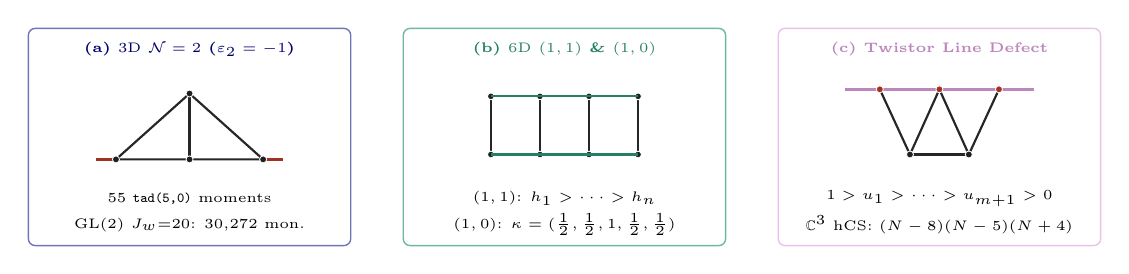
\begin{tikzpicture}[scale=0.89]
  % (a) 3D tadpole(5,0) + fan(2)
  \begin{scope}[xshift=-5.35cm]
    \draw[rounded corners=2.5pt, draw=NavyBlue!55, fill=white, line width=0.5pt] (-2.30,-1.55) rectangle (2.30,1.55);
    \node[font=\tiny\bfseries, text=NavyBlue!85!black] at (0,1.25) {(a) $3\mathrm{D}$ $\mathcal{N}=2$ ($\eps_2=-1$)};
    \coordinate (fh) at (0,0.62); \coordinate (fa) at (-1.05,-0.32); \coordinate (fb) at (0,-0.32); \coordinate (fc) at (1.05,-0.32);
    \draw[prop] (fh)--(fa)--(fb)--(fc)--(fh); \draw[prop] (fh)--(fb);
    \draw[extleg] (fa)--++(-0.28,0); \draw[extleg] (fc)--++(0.28,0);
    \foreach \pt in {fh,fa,fb,fc} \filldraw[v0] (\pt) circle (0.05cm);
    \node[font=\tiny] at (0,-0.88) {$55$ \texttt{tad(5,0)} moments};
    \node[font=\tiny] at (0,-1.25) {$\GL(2)$ $J_w{=}20$: $30{,}272$ mon.};
  \end{scope}
  % (b) 6D (1,1) box ladder & (1,0) unicyclic
  \begin{scope}[xshift=0cm]
    \draw[rounded corners=2.5pt, draw=PineGreen!55, fill=white, line width=0.5pt] (-2.30,-1.55) rectangle (2.30,1.55);
    \node[font=\tiny\bfseries, text=PineGreen!85!black] at (0,1.25) {(b) $6\mathrm{D}$ $(1,1)$ \& $(1,0)$};
    \foreach \idx/\xx in {0/-1.05, 1/-0.35, 2/0.35, 3/1.05} {
      \coordinate (u\idx) at (\xx,0.58); \coordinate (d\idx) at (\xx,-0.25);
      \draw[prop] (u\idx)--(d\idx);
      \filldraw[v0] (u\idx) circle (0.048cm); \filldraw[v0] (d\idx) circle (0.048cm);
    }
    \draw[prop, PineGreen!85!black] (u0)--(u1)--(u2)--(u3);
    \draw[prop, PineGreen!85!black] (d0)--(d1)--(d2)--(d3);
    \node[font=\tiny] at (0,-0.88) {$(1,1)$: $h_1>\dots>h_n$};
    \node[font=\tiny] at (0,-1.25) {$(1,0)$: $\kappa = (\frac{1}{2},\frac{1}{2},1,\frac{1}{2},\frac{1}{2})$};
  \end{scope}
  % (c) Twistor ordered line defect
  \begin{scope}[xshift=5.35cm]
    \draw[rounded corners=2.5pt, draw=Plum!65, fill=white, line width=0.5pt] (-2.30,-1.55) rectangle (2.30,1.55);
    \node[font=\tiny\bfseries, text=Plum!85!black] at (0,1.25) {(c) Twistor Line Defect};
    \draw[line width=1.2pt, draw=Plum!85!black] (-1.35,0.68)--(1.35,0.68);
    \coordinate (w1) at (-0.85,0.68); \coordinate (w2) at (0,0.68); \coordinate (w3) at (0.85,0.68);
    \coordinate (bv1) at (-0.42,-0.25); \coordinate (bv2) at (0.42,-0.25);
    \draw[prop] (w1)--(bv1); \draw[prop] (w2)--(bv1); \draw[prop] (w2)--(bv2); \draw[prop] (w3)--(bv2); \draw[prop] (bv1)--(bv2);
    \foreach \pt in {w1,w2,w3} \filldraw[vbiv] (\pt) circle (0.05cm);
    \filldraw[v0] (bv1) circle (0.05cm); \filldraw[v0] (bv2) circle (0.05cm);
    \node[font=\tiny] at (0,-0.88) {$1 > u_1 > \dots > u_{m+1} > 0$};
    \node[font=\tiny] at (0,-1.25) {$\C^3$ hCS: $(N-8)(N-5)(N+4)$};
  \end{scope}
\end{tikzpicture}
\caption{Multi-loop gauge-twist structures of Theorems~\ref{thm:3d-n2-complete} and~\ref{thm:6d-8d-twistor}: (a)~$3\mathrm{D}$ $\mathcal{N}=2$ supercharge graphs; (b)~$6\mathrm{D}$ $\mathcal{N}=(1,1)$ box ladders and $\mathcal{N}=(1,0)$ rank-$5$ weights; (c)~ordered twistor line-defect simplex and $6\mathrm{D}$ $\C^3$ $\fso_8$ factorization.}
\label{fig:3d-6d-gauge}
\end{figure}

% ============================================================================
\section{Minimal \texorpdfstring{$11\mathrm{D}$}{11D} Supergravity, Four-Loop Kodaira--Spencer/BCOV Gravity, and All-Order \texorpdfstring{$\mathcal{N}=4$}{N=4} Twisted Holography}
\label{sec:sugra-bcov-holo}
% ============================================================================

Pushing our perturbative $(H,T)$ engines from gauge theories into gravitational twists and AdS/CFT holography, we establish three multi-loop gravitational pillars---introducing each gravitational background card immediately ahead of the loop computation that uses it: (1)~the pure-spinor twist of physical eleven-dimensional supergravity followed by its two-loop $-\frac{63g}{256\pi^{10}}$ QME obstruction and further-twist Koszul $g$-torsion~\cite{CJS78,Cederwall10,RSW21,HPR25,Repo9e833c8}; (2)~Calabi--Yau polyvectors and minimal BCOV gravity followed by four-loop Kodaira--Spencer invariants, Type~I $\SO(32)$, and delayed genus-$4$ BCOV~\cite{BCOV94,CL19,LW26,Repo9e833c8}; and (3)~$\fpsl(3|3)$ super-polyvectors followed by all-order finite-$N$ and nonplanar $4\mathrm{D}$ $\mathcal{N}=4$ twisted holography~\cite{CG18,SW,FPW24,BG26,Repo9e833c8}.

\subsection{In-Situ Pure-Spinor \texorpdfstring{$11\mathrm{D}$}{11D} Twist, Two-Loop Obstruction, and Koszul \texorpdfstring{$g$}{g}-Torsion}
\label{subsec:11d-two-loop}
\phantomsection\label{subsec:11d-pure-spinor}

\begin{zkmodule}{From Physical $11\mathrm{D}$ Cremmer--Julia--Scherk Supergravity to $S_{E,11\mathrm{D}}$ and $E(5|10)$}{minimal-11d-sugra-e510-model}
Physical eleven-dimensional supergravity~\cite{CJS78} on $M_{11}$ has field multiplet $(e_M{}^{\underline{A}}, C_3, \Psi_M)$: elfbein $e_M{}^{\underline{A}}$ ($44$ on-shell bosonic states), $3$-form gauge potential $C_3$ with curvature $G_4 := \dd C_3$ ($84$ states), and Majorana gravitino $1$-form $\Psi_M^\alpha$ ($\alpha \in \{1,\dots,32\}$, $128$ fermionic states), governed by
\begin{equation}
\label{eq:cjs-action}
\begin{aligned}
S_{\mathrm{CJS}}[e,C_3,\Psi] = \frac{1}{2\kappa_{11}^2}\int_{M_{11}}\!\Bigl(&eR\,\dd^{11}x - \tfrac{1}{2}G_4\wedge *G_4 - \tfrac{1}{6}C_3\wedge G_4\wedge G_4\\
&-\ii e\bar{\Psi}_M\Gamma^{MNP}D_N\Psi_P\,\dd^{11}x + \mathcal{O}(\Psi^2 G_4, \Psi^4)\Bigr),
\end{aligned}
\end{equation}
invariant under $\delta_\epsilon e_M{}^{\underline{A}} = \ii\bar{\epsilon}\Gamma^{\underline{A}}\Psi_M$, $\delta_\epsilon C_{MNP} = -3\ii\bar{\epsilon}\Gamma_{[MN}\Psi_{P]}$, and $\delta_\epsilon\Psi_M = \widehat{\nabla}_M\epsilon$, whose off-shell Rarita--Schwinger commutator non-closure is completed in BV by bosonic SUSY ghost $\chi^\alpha$ and quadratic gravitino antifields $\frac{1}{2}\Psi^{\ddagger M}\mathcal{R}_{MN}(\chi)\Psi^{\ddagger N}$~\cite{Cederwall10,RSW21}.
\end{zkmodule}

\begin{theorem}[Pure-spinor derivation of minimal twisted $11\mathrm{D}$ supergravity and Kac's $E(5|10)$~{\cite{Cederwall10,RSW21}}]
\label{thm:11d-from-scratch}
Linearize~\eqref{eq:cjs-action} around $M_{11} = \RR_\tau \times \C^5_z$ ($V := T^{1,0}\C^5 \cong \C^5$, $\Omega := \dd z^1\wedge\cdots\wedge\dd z^5$, $\mathcal{A}^\bullet := \Omega^\bullet(\RR_\tau)\widehat{\otimes}\Omega^{0,\bullet}(\C^5)$) and realize the $32$-component $\Spin(11,\C)$ spinor module as the Fock exterior algebra $S_{32} \cong \bigoplus_{\substack{p\in\{0,\dots,5\}\\\mathrm{form\ degree}}}\Lambda^p V^*$ ($1+5+10+10+5+1 = 32$) with Clifford operators $\Gamma_i = \sqrt{2}\,\iota_{\partial_i}$, $\Gamma_{\bar{\imath}} = \sqrt{2}\,\dd\bar{z}^{\bar{\imath}}\wedge\cdot$, $\Gamma_\tau = (-1)^p$, and Mukai pairing $C(\eta_1,\eta_2) := (-1)^{\binom{p}{2}}[\eta_1\wedge\eta_2]_{\Lambda^5 V^*}$.
\begin{enumerate}[label=(\arabic*),leftmargin=*]
  \item Selecting the $\SU(5)$-invariant pure spinor $q := \mathbf{1} \in \Lambda^0 V^*$ satisfies $C(q,\Gamma^M q) = [\mathbf{1}\wedge\Gamma^M\mathbf{1}]_{\Lambda^5 V^*} = 0$ ($\deg \le 1 < 5 \implies Q_q^2 = 0$), $\Gamma_i q = 0$ (preserving holomorphic $\partial_{z^1},\dots,\partial_{z^5}$), and $\Gamma_\tau q = \mathbf{1}$, $\Gamma_{\bar{\imath}}q = \sqrt{2}\dd\bar{z}^{\bar{\imath}}$ (rendering $\partial_\tau, \dbar_{\bar{1}},\dots,\dbar_{\bar{5}}$ exact).
  \item Eliminating the $Q_q$-contractible metric/gravitino and $C_3$/gravitino pairs retains four $\mathcal{A}^\bullet$-superfields $(\mu^i, \gamma_i, \beta, \nu)$ ($\mu^i \in \mathcal{A}^1\otimes V$, $\gamma_i\,\dd z^i \in \Omega^{1,0}(\C^5)\otimes\mathcal{A}^2$, $\beta \in \mathcal{A}^3$, $\nu \in \mathcal{A}^0$), on which $-\frac{1}{6}\int C_3\wedge\dd C_3\wedge\dd C_3$ wedges $(1+2+2)=5$ $\dd z$'s and $(2+2+2)=6$ $(\tau,\bar{z})$-degrees directly into ($D_{\mathrm{free}} = \dd_\tau + \dbar$):
  \begin{equation}
  \label{eq:11d-twisted-action}
  \begin{aligned}
  S_{E,11\mathrm{D}}[\mu,\gamma,\beta,\nu] = \int_{\RR\times\C^5}\Omega\wedge\Bigl[&\gamma_i D_{\mathrm{free}}\mu^i + \beta D_{\mathrm{free}}\nu + \beta\,\partial_i\mu^i\\
  &+ \frac{1}{1-\nu}\mu^i\mu^j\partial_i\gamma_j + \frac{g}{6}\eps^{ijklm}\gamma_i\partial_j\gamma_k\partial_l\gamma_m\Bigr].
  \end{aligned}
  \end{equation}
  \item Setting $X^i := (1-\nu)^{-1}\mu^i$ and integrating out $(\beta,\nu)$ enforces $\partial_i X^i = 0$ and realizes Kac's exceptional infinite-dimensional simple Lie superalgebra $E(5|10) = E(5|10)_{\mathrm{even}}\oplus E(5|10)_{\mathrm{odd}}$ ($E(5|10)_{\mathrm{even}} = \{X^i(z)\partial_i : \partial_i X^i = 0\}$, $E(5|10)_{\mathrm{odd}} = \{F = \frac{1}{2}F_{ij}(z)\dd z^i\wedge\dd z^j : \partial_{[k}F_{ij]} = 0\}$) with odd-odd bracket $[F,\widetilde{F}]^i = \frac{1}{4}\eps^{ijklm}F_{jk}\widetilde{F}_{lm}$ satisfying $\partial_i[F,\widetilde{F}]^i = 0$ identically by $\dd F = \dd\widetilde{F} = 0$.
\end{enumerate}
\end{theorem}

\begin{proof}\leavevmode
\begin{proofpart}{Claim 1: Pure-spinor nilpotency and exact translations}
From $\{\Gamma_i,\Gamma_{\bar{\jmath}}\} = 2\delta_{i\bar{\jmath}}$ and $\Gamma_\tau^2 = \mathbf{1}$, the Fock operators furnish $\mathrm{Cl}(11,\C)$. Because $\mathbf{1} \in \Lambda^0 V^*$ and $\Gamma^M\mathbf{1} \in \Lambda^0 V^*\oplus\Lambda^1 V^*$, the top $\Lambda^5 V^*$ component of $\mathbf{1}\wedge\Gamma^M\mathbf{1}$ vanishes identically, proving $Q_q^2 = 0$; $\{Q_q, \widehat{Q}_\eta\} = C(q,\Gamma^M\eta)\partial_M$ hits $\partial_\tau$ (via $\eta \in \Lambda^5 V^*$) and $\dbar_{\bar{\imath}}$ (via $\eta \in \Lambda^4 V^*$).
\end{proofpart}
\begin{proofpart}{Claim 2: Doublet elimination and $(3+4+4=11)$ CJS descent}
Under $\delta_q e_M{}^{\underline{A}} = \ii C(q,\Gamma^{\underline{A}}\Psi_M)$ and $\delta_q C_{MNP} = -3\ii C(q,\Gamma_{[MN}\Psi_{P]})$, $\Psi_{\Lambda^{4,5}}$ pairs with $(h_{M\tau}, h_{M\bar{\jmath}})$ and $\Psi_{\Lambda^3}$ pairs with $C_{\bar{\imath}\bar{\jmath}P}$. On $C_3^{\mathrm{surv}} = \gamma_i\,\dd z^i$, $\dd C_3^{\mathrm{surv}} = \partial_j\gamma_k\,\dd z^j\wedge\dd z^k + D_{\mathrm{free}}\gamma_k\wedge\dd z^k$, so $C_3^{\mathrm{surv}}\wedge(\dd C_3^{\mathrm{surv}})^2$ saturates $\Omega = \dd^5 z$ via $\gamma_i\partial_j\gamma_k\partial_l\gamma_m\,\eps^{ijklm}\Omega$, yielding~\eqref{eq:11d-twisted-action} (Figure~\ref{fig:11d-fock-spinor}).
\end{proofpart}
\begin{proofpart}{Claim 3: Closure of Kac's $E(5|10)$}
Differentiating $[F,\widetilde{F}]^i = \frac{1}{4}\eps^{ijklm}F_{jk}\widetilde{F}_{lm}$ gives $\partial_i[F,\widetilde{F}]^i = \frac{1}{4}\eps^{ijklm}(\partial_i F_{jk})\widetilde{F}_{lm} + \frac{1}{4}\eps^{ijklm}F_{jk}(\partial_i\widetilde{F}_{lm}) = 0$ because $\eps^{ijklm}\partial_i F_{jk} = \eps^{ijklm}\partial_{[i}F_{jk]} = 0$ on $\dd$-closed $2$-forms $F, \widetilde{F}$.
\end{proofpart}
\end{proof}

\begin{figure}[H]
\centering
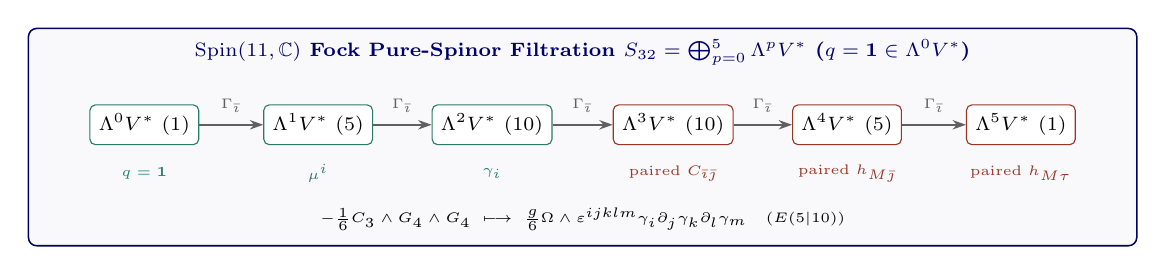
\begin{tikzpicture}[scale=0.92]
  \draw[rounded corners=3pt, draw=NavyBlue!75!black, fill=NavyBlue!2.5, line width=0.55pt] (-7.65,-1.45) rectangle (7.65,1.55);
  \node[font=\scriptsize\bfseries, text=NavyBlue!85!black] at (0,1.22) {$\Spin(11,\C)$ Fock Pure-Spinor Filtration $S_{32} = \bigoplus_{p=0}^5 \Lambda^p V^*$ ($q = \mathbf{1} \in \Lambda^0 V^*$)};
  \foreach \pp/\xx/\dimv/\col/\tag in {
    0/-6.05/1/PineGreen!85!black/{$q=\mathbf{1}$},
    1/-3.65/5/PineGreen!80!black/{$\mu^i$},
    2/-1.25/10/PineGreen!80!black/{$\gamma_i$},
    3/ 1.25/10/BrickRed!80!black/{paired $C_{\bar{\imath}\bar{\jmath}}$},
    4/ 3.65/5/BrickRed!80!black/{paired $h_{M\bar{\jmath}}$},
    5/ 6.05/1/BrickRed!80!black/{paired $h_{M\tau}$}%
  } {
    \node[draw=\col, rounded corners=2pt, fill=white, inner sep=3.2pt, font=\scriptsize] (L\pp) at (\xx,0.22) {$\Lambda^{\pp}V^*$ ($\dimv$)};
    \node[font=\tiny, text=\col] at (\xx,-0.45) {\tag};
  }
  \foreach \a/\b in {0/1,1/2,2/3,3/4,4/5} {
    \draw[-{Stealth[length=1.7mm,width=1.2mm]}, line width=0.55pt, gray!75!black] (L\a.east) -- node[above=1pt, font=\tiny] {$\Gamma_{\bar{\imath}}$} (L\b.west);
  }
  \node[font=\tiny] at (0,-1.08) {$-\frac{1}{6}C_3\wedge G_4\wedge G_4 \;\longmapsto\; \frac{g}{6}\Omega\wedge\eps^{ijklm}\gamma_i\partial_j\gamma_k\partial_l\gamma_m\quad (E(5|10))$};
\end{tikzpicture}
\caption{In-situ $\SU(5)$ exterior grading of the $32$-component $\Spin(11,\C)$ spinor representation (Background Card~7.1 and Theorem~\ref{thm:11d-from-scratch}): $\Lambda^{3,4,5}V^*$ form $Q_q$-contractible pairs, whereas $\Lambda^{0,1,2}V^*$ retain $(\nu,\mu^i,\gamma_i,\beta)$ and descend the CJS topological coupling directly to $E(5|10)$.}
\label{fig:11d-fock-spinor}
\end{figure}

\begin{theorem}[Two-loop $-\frac{63g}{256\pi^{10}}$ obstruction, rank-$80\to 83$ self-bracket elimination, and further-twist $g$-torsion~{\cite{RSW21,HPR25,Repo9e833c8}}]
\label{thm:11d-obstruction}
In minimal twisted $11\mathrm{D}$ supergravity~\eqref{eq:11d-twisted-action} on $\RR_\tau\times\C^5_z$ ($H=5, T=1, D=6$):
\begin{enumerate}[label=(\arabic*),leftmargin=*]
  \item \emph{Exact $1008\pi$ pairing across all five $12$-vertex theta topologies:} Odd loops vanish ($O_{2m+1}=0$). At two loops ($|V|=12, |I|=13$, five tight topologies $\theta(1,6,6), \theta(2,5,6), \theta(3,4,6), \theta(3,5,5), \theta(4,4,5)$, Figure~\ref{fig:11d-thetas} and Table~\ref{tab:11d-theta-pairings}), $\beta\partial_i\mu^i$ decouples by column linearity of $D_\theta$ and all $65$ zero-time contacts vanish. Evaluated on the $Q_0$-closed $23$-derivative balanced cycle $\mathcal{Z}_{3+6}$ ($\mu^9\gamma^1$) via $99$-bit multi-prime CRT across $2{,}160$ path partitions, the five fractional contributions sum to the \textbf{exact integer multiple $1008\pi$}:
  \begin{equation}
  \label{eq:11d-63-pairing}
  \bigl\langle O_2^{(g=1)},\, \mathcal{Z}_{3+6}\bigr\rangle_{\mathrm{unrooted}} = -\frac{1008\pi\,g}{4096\pi^{11}} = -\frac{63g}{256\pi^{10}} \neq 0,\qquad
  \bigl\langle Q_2\mathcal{I},\, \mathcal{Z}_{3+6}\bigr\rangle_{\mathrm{rooted}} = -\frac{189g}{64\pi^{10}},
  \end{equation}
  descending to a nonzero class in $H^{15}_{\mathrm{GF}}(E(5|10))/(\kappa H^{12}_{\mathrm{GF}}(E(5|10)))$.

  \item \emph{Elimination of $\frac{1}{2}\{I_1,I_1\}|_{\mathcal{O}(g)}$:} For any $Q_0$-closed homogeneous full-wedge $1$-loop counterterm $I_1 = I_1^{(0)} + g I_1^{(1)} + \cdots$, outgoing $Q_0$ on the $83$-dimensional $I_1^{(1)}$ symbol space has rank $80$ and \textbf{jumps to $83$} upon adjoining $Q_g(I_1^{(0)})$ ($\dim I_1^{(0)} = 3$), forcing $I_1^{(0)} = 0$ and $\frac{1}{2}\{I_1,I_1\}|_{\mathcal{O}(g)} = 0$ on $\mathcal{Z}_{3+6}$.

  \item \emph{Compact $T^{2r}\times\C^{5-r}$ routing and further-twist Koszul $g$-torsion:} On $S^1\times T^{2r}\times\C^{5-r}$ ($1\le r\le 5$), compact rank equals $\dim\Span A + \dim\Span B + \dim\Span C - \dim(\Span A\cap\Span B\cap\Span C)$, requiring $\ge 2r$ compact-momentum slots (attained sharply on $\theta(1,6,6)$ with $K_{166} = -\frac{\pi}{158400}$, vanishing on zero modes). In RSW's constant-$2$-form further twist $\delta X = -p\wedge\iota_X(\dd z^1\wedge\dd z^2)$, $\delta F = g(\dd z^1\wedge\dd z^2\wedge F)^\sharp$ (fixed-momentum strata $p|_{\C^3}\neq 0 \mapsto (0,0)$, $p|_{\C^3}=0,p\neq 0 \mapsto (4,4)$, $p=0 \mapsto (2,7)$), the normal-momentum complex over $R = \C[g,q_3,q_4,q_5]$ is $0 \to R \xrightarrow{q} R^3 \xrightarrow{g\,q\wedge} R^3 \xrightarrow{q\cdot} R \to 0$, carrying $g$-torsion $H^{\mathrm{even}} = \ker(q\cdot)/(g\,\ker(q\cdot))$ ($\dim_{\C}(H^{\mathrm{even}})_m = m(m+2)$), zero-momentum fiber $\Tor_j^R = \Lambda^j\C^3$, and $H^{\mathrm{even}}|_{q_3=t,q_{4,5}=0} = (\C[g,t]/(gt))^2$ forbidding any translation-invariant finite-jet contraction $\delta h + h\delta = \id$.
\end{enumerate}
\end{theorem}

\begin{proof}
Theorem~\ref{thm:theta-closed} evaluates the five $(5,1)$ theta kernels, summed over $2{,}160$ partitions on $\mathcal{Z}_{3+6}$ in~(1). Bareiss elimination modulo $1009$ and $251$ proves the $80 \to 83$ rank jump in~(2). Kernel calculation on $(a,b,c)\mapsto(a+b,b+c)$ and homology of $g\,q\wedge\cdot$ over $R$ prove~(3).
\end{proof}

\begin{table}[H]
\centering
\scriptsize
\setlength{\tabcolsep}{5pt}
\renewcommand{\arraystretch}{1.15}
\begin{tabular}{@{}lcrr@{}}
\toprule
\textbf{Theta Topology} & \textbf{Geometric Kernel $K/\pi$ at $(5,1)$} & \textbf{Symmetry $|\Aut|$} & \textbf{Exact Cycle Pairing on $\mathcal{Z}_{3+6}$ (times $\pi$)} \\
\midrule
$\theta(1,6,6)$ & $-\frac{1}{158400}$ & $2$ & $+\frac{3568529267}{12168702}$ \\
$\theta(2,5,6)$ & $+\frac{1}{249480}$ & $1$ & $+\frac{390374345071}{1338557220}$ \\
$\theta(3,4,6)$ & $-\frac{1}{266112}$ & $1$ & $+\frac{130687286941}{514829700}$ \\
$\theta(3,5,5)$ & $+\frac{1}{532224}$ & $2$ & $+\frac{1673839750871}{20078358300}$ \\
$\theta(4,4,5)$ & $-\frac{1}{498960}$ & $2$ & $+\frac{344930551643}{4015671660}$ \\
\midrule
\textbf{Total Sum} & $5$ tight $6$-Laman shapes ($2{,}160$ partitions) & --- & $\mathbf{1008}\quad\bigl(\implies O_2 = -\frac{1008\pi g}{4096\pi^{11}} = -\frac{63g}{256\pi^{10}}\bigr)$ \\
\bottomrule
\end{tabular}
\caption{Exact fractional cancellation across all five $12$-vertex two-loop theta topologies of minimal twisted $11\mathrm{D}$ supergravity summing to $1008\pi$ on $\mathcal{Z}_{3+6}$~\cite{Repo9e833c8}.}
\label{tab:11d-theta-pairings}
\end{table}

\begin{figure}[H]
\centering
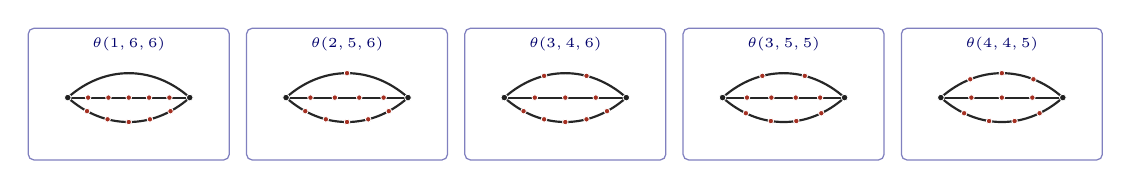
\begin{tikzpicture}[scale=0.88]
  \foreach \xx/\lbl/\nA/\nB/\nC in {
    -6.30/{\theta(1,6,6)}/0/5/5,
    -3.15/{\theta(2,5,6)}/1/4/5,
     0.00/{\theta(3,4,6)}/2/3/5,
     3.15/{\theta(3,5,5)}/2/4/4,
     6.30/{\theta(4,4,5)}/3/3/4%
  } {
    \begin{scope}[shift={(\xx, 0)}]
      \draw[rounded corners=2pt, draw=NavyBlue!50, fill=white, line width=0.45pt] (-1.45,-0.95) rectangle (1.45,0.95);
      \node[font=\tiny\bfseries, text=NavyBlue!85!black] at (0,0.72) {$\lbl$};
      \coordinate (tl) at (-0.88,-0.05); \coordinate (tr) at (0.88,-0.05);
      \draw[prop] (tl) .. controls (-0.35,0.42) and (0.35,0.42) .. (tr);
      \draw[prop] (tl)--(tr);
      \draw[prop] (tl) .. controls (-0.35,-0.52) and (0.35,-0.52) .. (tr);
      \filldraw[v0] (tl) circle (0.048cm); \filldraw[v0] (tr) circle (0.048cm);
      \ifnum\nA>0
        \foreach \k in {1,...,\nA} {
          \pgfmathsetmacro{\tt}{\k/(\nA+1)}
          \path (tl) .. controls (-0.35,0.42) and (0.35,0.42) .. coordinate[pos=\tt] (pa) (tr);
          \filldraw[vbiv] (pa) circle (0.04cm);
        }
      \fi
      \foreach \k in {1,...,\nB} {
        \pgfmathsetmacro{\tt}{\k/(\nB+1)}
        \path (tl) -- coordinate[pos=\tt] (pb) (tr);
        \filldraw[vbiv] (pb) circle (0.04cm);
      }
      \foreach \k in {1,...,\nC} {
        \pgfmathsetmacro{\tt}{\k/(\nC+1)}
        \path (tl) .. controls (-0.35,-0.52) and (0.35,-0.52) .. coordinate[pos=\tt] (pc) (tr);
        \filldraw[vbiv] (pc) circle (0.04cm);
      }
    \end{scope}
  }
\end{tikzpicture}
\caption{All five $6$-Laman two-loop theta Feynman topologies of minimal twisted $11\mathrm{D}$ supergravity ($|V|=12, |I|=13$, $10$ red bivalent source insertions per graph), summing to $1008\pi$ and $-\frac{63g}{256\pi^{10}}$ on $\mathcal{Z}_{3+6}$ (Theorem~\ref{thm:11d-obstruction}).}
\label{fig:11d-thetas}
\end{figure}

\subsection{In-Situ BCOV Background, Four-Loop Kodaira--Spencer \texorpdfstring{$D_4 > 0$}{D\_4 > 0}, and Delayed Genus-\texorpdfstring{$4$}{4} BCOV}
\label{subsec:ks-type1-bcov}
\phantomsection\label{subsec:bcov-lecture}

\begin{zkmodule}{Kodaira--Spencer Gravity, Tian--Todorov Divergence, and Minimal BCOV Theory}{ks-type1-wzw4-minimal-bcov}
Whereas open topological B-model strings on a Calabi--Yau $d$-fold $(Y,\Omega)$ ($d=3$ or $d=5$, $\Omega = \dd z^1\wedge\cdots\wedge\dd z^d$ on $\C^d$) yield holomorphic Chern--Simons gauge theory, closed B-model strings govern deformations of complex structure and generalized Calabi--Yau geometry via \emph{Bershadsky--Cecotti--Ooguri--Vafa (BCOV) theory}~\cite{BCOV94,CL19}.

\paragraph{1.\ Polyvector fields $\mathrm{PV}^{p,q}(\C^d)$, Calabi--Yau contraction $A_\Omega$, and Tian--Todorov divergence $\partial_\Omega$.}
A $(p,q)$-polyvector field $\alpha \in \mathrm{PV}^{p,q}(\C^d) := \Omega^{0,q}(\C^d, \Lambda^p T^{1,0}\C^d)$ has total cohomological degree $|\alpha| = p + q$. Contracting polyvectors into $\Omega$ defines a linear isomorphism $A_\Omega : \mathrm{PV}^{p,q}(\C^d) \xrightarrow{\cong} \Omega^{d-p,q}(\C^d)$ via $A_\Omega(\alpha) := \iota_\alpha\Omega$, transporting $\partial : \Omega^{d-p,q} \to \Omega^{d-p+1,q}$ back to the \emph{Calabi--Yau divergence operator} $\partial_\Omega := A_\Omega^{-1}\circ\partial\circ A_\Omega : \mathrm{PV}^{p,q} \to \mathrm{PV}^{p-1,q}$ ($\partial_\Omega^2 = 0$; on Beltrami differentials $\mu = \mu^i\partial_i \in \mathrm{PV}^{1,\bullet}$, $\partial_\Omega\mu = \partial_i\mu^i$).

\paragraph{2.\ Heat-kernel resolution of the nonlocal $\dbar\partial_\Omega^{-1}$ kinetic term.}
Restricting to $\ker\partial_\Omega$ produces the nonlocal BCOV kinetic pairing $S_{E,\mathrm{BCOV,kin}}[\mu] = \frac{1}{2}\int_{\C^d}\Omega\wedge A_\Omega(\mu\wedge\dbar\partial_\Omega^{-1}\mu)$ alongside $\frac{1}{6}\int_{\C^d}\Omega\wedge A_\Omega(\mu\wedge\mu\wedge\mu)$ ($d=3$ Kodaira--Spencer gravity~\cite{BCOV94}). Costello and Li~\cite{CL19} resolve $\partial_\Omega^{-1}$ without nonlocality via the gauge-fixing operator $D^*_{\mathrm{BCOV}} := \partial_\Omega\dbar^*$: $\partial_\Omega$ cancels $\partial_\Omega^{-1}$, yielding the \emph{local derivative-carrying propagator} $P_{\mathrm{BCOV}}(\eps,L) = \int_\eps^L \dd t\,(\partial_\Omega\dbar^*)[K_t]_\Omega$!

\paragraph{3.\ Minimal BCOV on $\C^5$ $=$ Twisted $10\mathrm{D}$ Type~IIB Supergravity and $\mathrm{D}3$-brane flux.}
On $\C^5$ ($H=5, T=0$), Costello--Li~\cite{CL19} identify $\mathrm{PV}^{\bullet,\bullet}(\C^5)[[u]]$ ($u$ of degree $+2$ encoding worldsheet gravitational descendants with $Q_{\mathrm{BCOV}} = \dbar + u\partial_\Omega$) with the holomorphic twist of physical $10\mathrm{D}$ Type~IIB supergravity: $\phi \in \mathrm{PV}^{0,\bullet}$ is the chiral axio-dilaton/RR $0$-form, $\mu^i\partial_i \in \mathrm{PV}^{1,\bullet}_{\mathrm{div}=0}$ packages metric and $B$-field complex-structure deformations, and $\frac{1}{2}\alpha^{ij}\partial_i\wedge\partial_j \in \mathrm{PV}^{2,\bullet}_{\mathrm{div}=0}$ encodes the self-dual Ramond--Ramond $4$-form ($F_5^{\mathrm{SD}} = \partial A_\Omega(\alpha)$). Placing $N$ $\mathrm{D}3$-branes along $\C^2_z \subset \C^2_z\times\C^3_w$ sources the Bochner--Martinelli RR flux $N F_{\mathrm{BM}}$ on $\C^5\setminus\C^2$ ($\dbar F_{\mathrm{BM}} = \delta_{\C^2}$, $F_{\mathrm{BM}} := \frac{1}{4\pi^2}\partial_{z^1}\wedge\partial_{z^2}\,\eps_{\bar{\imath}\bar{\jmath}\bar{k}}\bar{w}^{\bar{\imath}}\dd\bar{w}^{\bar{\jmath}}\wedge\dd\bar{w}^{\bar{k}}/|w|^6$), deforming the bulk differential to $\dbar + u\partial_\Omega + N[F_{\mathrm{BM}}, -]_{\mathrm{SN}}$ in Costello--Gaiotto twisted holography~\cite{CG18} (Figure~\ref{fig:bcov-geometry}).
\end{zkmodule}

\begin{lemma}[Tian--Todorov BV identity and Kodaira--Spencer Maurer--Cartan closure~{\cite{TT87,BCOV94}}]
\label{lem:tian-todorov}
On $\mathrm{PV}^{\bullet,\bullet}(\C^d)$, $\partial_\Omega$ fails to be a derivation of the exterior wedge product precisely by the Schouten--Nijenhuis bracket:
\begin{equation}
\label{eq:tian-todorov}
(-1)^{|\alpha|-1}[\alpha, \beta]_{\mathrm{SN}} = \partial_\Omega(\alpha\wedge\beta) - (\partial_\Omega\alpha)\wedge\beta - (-1)^{|\alpha|}\alpha\wedge(\partial_\Omega\beta).
\end{equation}
Consequently, any divergence-free Beltrami differential $\mu \in \mathrm{PV}^{1,1}(\C^3)$ ($\partial_\Omega\mu = 0$) satisfies $\dbar_\mu^2 := (\dbar + \mu^i\partial_i)^2 = 0$ precisely when $\dbar\mu + \frac{1}{2}[\mu,\mu]_{\mathrm{SN}} = 0$, generated as the Euler--Lagrange equation of $\frac{1}{6}\int_{\C^3}\Omega\wedge A_\Omega(\mu\wedge\mu\wedge\mu)$.
\end{lemma}

\begin{proof}\leavevmode
\begin{proofpart}{Claim 1: Tian--Todorov identity}
By $\Omega^{0,\bullet}$-linearity, check on holomorphic vector fields $X = X^i\partial_i$ ($|\alpha|=1$, $\partial_\Omega X = \partial_i X^i$) and $Y = Y^j\partial_j$: $\partial\iota_{X\wedge Y}\Omega$ gives $\partial_\Omega(X\wedge Y) = [\partial_i(X^i Y^j) - \partial_i(X^j Y^i)]\partial_j = (\partial_\Omega X)Y - X(\partial_\Omega Y) + [X,Y]_{\mathrm{SN}}$, extending to higher $p$ by the odd Poisson Leibniz rule.
\end{proofpart}
\begin{proofpart}{Claim 2: Maurer--Cartan closure from the cubic BCOV interaction}
Acting on $z^k$, $\dbar_\mu^2 z^k = \dbar\mu^k + \frac{1}{2}[\mu,\mu]_{\mathrm{SN}}^k$ since $|\mu| = 2$ is even. Applying~\eqref{eq:tian-todorov} with $\partial_\Omega\mu = 0$ gives $\partial_\Omega(\mu\wedge\mu) = -[\mu,\mu]_{\mathrm{SN}}$ and $\partial_\Omega(\mu\wedge\mu\wedge\mu) = -3[\mu,\mu]_{\mathrm{SN}}\wedge\mu$, so varying $\frac{1}{6}\int_{\C^3}\Omega\wedge A_\Omega(\mu\wedge\mu\wedge\mu)$ reproduces $\frac{1}{2}[\mu,\mu]_{\mathrm{SN}}$.
\end{proofpart}
\end{proof}

\begin{figure}[H]
\centering
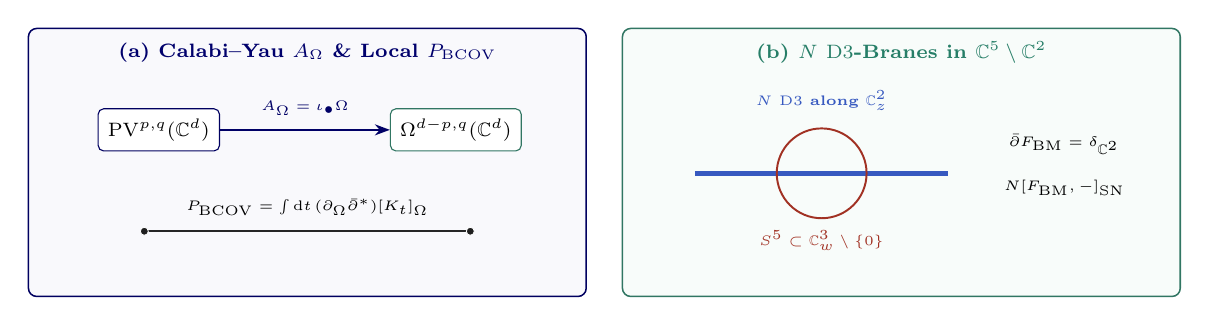
\begin{tikzpicture}[scale=0.92]
  % Left: Polyvector contraction & heat-kernel propagator
  \begin{scope}[shift={(-4.10,0)}]
    \draw[rounded corners=3pt, draw=NavyBlue!75!black, fill=NavyBlue!2.5, line width=0.55pt] (-3.85,-1.85) rectangle (3.85,1.85);
    \node[font=\scriptsize\bfseries, text=NavyBlue!85!black] at (0,1.52) {(a) Calabi--Yau $A_\Omega$ \& Local $P_{\mathrm{BCOV}}$};
    \node[draw=NavyBlue!75!black, rounded corners=2pt, fill=white, inner sep=3.5pt, font=\scriptsize] (PV) at (-2.05,0.45) {$\mathrm{PV}^{p,q}(\C^d)$};
    \node[draw=PineGreen!75!black, rounded corners=2pt, fill=white, inner sep=3.5pt, font=\scriptsize] (OM) at ( 2.05,0.45) {$\Omega^{d-p,q}(\C^d)$};
    \draw[-{Stealth[length=1.9mm,width=1.4mm]}, line width=0.65pt, NavyBlue!80!black] (PV) -- node[above=1.5pt, font=\tiny] {$A_\Omega = \iota_\bullet\Omega$} (OM);
    \draw[prop] (-2.25,-0.95) -- node[above=2pt, font=\tiny] {$P_{\mathrm{BCOV}} = \int\dd t\,(\partial_\Omega\dbar^*)[K_t]_\Omega$} (2.25,-0.95);
    \filldraw[v0] (-2.25,-0.95) circle (0.055cm);
    \filldraw[v0] ( 2.25,-0.95) circle (0.055cm);
  \end{scope}

  % Right: D3-brane stack in C^2_z x (C^3_w \setminus 0)
  \begin{scope}[shift={(4.10,0)}]
    \draw[rounded corners=3pt, draw=PineGreen!75!black, fill=PineGreen!2.5, line width=0.55pt] (-3.85,-1.85) rectangle (3.85,1.85);
    \node[font=\scriptsize\bfseries, text=PineGreen!85!black] at (0,1.52) {(b) $N$ $\mathrm{D}3$-Branes in $\C^5\setminus\C^2$};
    \draw[line width=1.6pt, draw=RoyalBlue!85!black] (-2.85,-0.15) -- (0.65,-0.15);
    \node[font=\tiny\bfseries, text=RoyalBlue!85!black] at (-1.10,0.85) {$N\ \mathrm{D}3$ along $\C^2_z$};
    \draw[->, line width=0.7pt, BrickRed!85!black] (-1.10,-0.15) circle (0.62cm);
    \node[font=\tiny, text=BrickRed!85!black] at (-1.10,-1.08) {$S^5 \subset \C^3_w\setminus\{0\}$};
    \node[font=\tiny] at (2.25, 0.25) {$\dbar F_{\mathrm{BM}} = \delta_{\C^2}$};
    \node[font=\tiny] at (2.25,-0.35) {$N[F_{\mathrm{BM}}, -]_{\mathrm{SN}}$};
  \end{scope}
\end{tikzpicture}
\caption{Geometric ingredients of Background Card~7.2: (a)~Calabi--Yau contraction $A_\Omega$ and local derivative-carrying propagator $P_{\mathrm{BCOV}}$ cancelling $\partial_\Omega^{-1}$; (b)~transverse $S^5 \subset \C^3_w\setminus\{0\}$ linking $N$ $\mathrm{D}3$-branes along $\C^2_z$ and sourcing the Bochner--Martinelli flux $N F_{\mathrm{BM}}$.}
\label{fig:bcov-geometry}
\end{figure}

\begin{theorem}[Four-loop Kodaira--Spencer $D_4$, Type~I $\SO(32)$, $\mathrm{WZW}_4$, and delayed $g=4$ BCOV~{\cite{CL19,LW26,Repo9e833c8}}]
\label{thm:ks-bcov}
\leavevmode
\begin{enumerate}[label=(\arabic*),leftmargin=*]
  \item \emph{Kodaira--Spencer on $\C^3$ and $\C^3\times K3/T^4$:} Tensoring with $H^\bullet(K3)$ or $H^\bullet(T^4)$ assigns connected $n$-loop bulk graphs external $R$-degree $4(1-n) < 0$, killing all $n \ge 2$ bulk loops identically~\cite{FPW24}. On minimal $\C^3$, $\iota_{p^{(q)}}F_q = 0$ cancels all $4$-primary contacts, while with one descendant $\psi_i$ ($D_1 = \frac{1}{24}, D_2 = \frac{1}{9720}, D_3 = \frac{411065203}{94152554496000}-\frac{3617}{1009008000}\zeta(3)$), summing all $50$ four-loop graphs yields
  \begin{equation}
  \label{eq:ks-D4-value}
  D_4 = \frac{192761752316371576853}{26469813789619200000000} + \frac{39781234295806109}{204242390352000000}\zeta(3) - \frac{411294138769}{13894040160000}\zeta(5) > 0.
  \end{equation}

  \item \emph{Type~I $\SO(32)$ two-loop hexagon and $\mathrm{WZW}_4$ finiteness:} Adjoining the two-loop open-closed mixed hexagon ($-\frac{1}{8640}$) to the four $8$-gluon theta graphs on $\C^5$ yields $84$ residual polynomials with monic $\gcd = N - 32$~\cite{CL19}; in flat $4\mathrm{D}$ $\mathrm{WZW}_4$, two-loop logarithmic UV poles cancel in both two-cubic and cubic-quartic sectors for every compact simple $G$.

  \item \emph{Minimal BCOV Ax--Schanuel positivity, delayed genus-$4$ response, and $g=4..6$ Ward targets:} In Li--Wang quantization~\cite{LW26}, $Q_g\phi > 0$ ($g \ge 2$) on real conserved waves $P = (p^{(1)},\dots,p^{(2g+3)})$ precisely when $\rk P = 5$ and $|T| \le g\,\rk\{p^{(q)} : q \in T\}$ ($\forall\,\varnothing\neq T$). On three scalar descendants $A_{k_1}, A_{k_2}, A_{k_3}$ ($k_1+k_2+k_3=4$) weighted by $C_{(4,0,0)}=2, C_{(3,1,0)}=-1, C_{(2,2,0)}=1, C_{(2,1,1)}=0$, donor-fusion identities $C_{\ell_1+1,\ell_2,\ell_3}+C_{\ell_1,\ell_2+1,\ell_3}+C_{\ell_1,\ell_2,\ell_3+1}=0$ ($\ell_1+\ell_2+\ell_3=3$) and vertical Abel rank $3g < 2g+4$ kill $g=0,1,2,3$ and first turn on at $g = 4$ via $6V_{4;(4,0,0)}-6V_{4;(3,1,0)}+3V_{4;(2,2,0)} = -\frac{31}{1024192512000}$ on multiplicity $(3,3,4)$:
  \begin{equation}
  \label{eq:delayed-g4-bcov}
  \begin{aligned}
  Q_0\phi(0) &= Q_1\phi(0) = Q_2\phi(0) = Q_3\phi(0) = 0,\\
  (2\pi\ii)^{20}Q_4\phi(0) &= \frac{(4!)^3}{3!\,3!\,4!}\cdot\frac{31}{1024192512000} = \frac{31}{64012032000},
  \end{aligned}
  \end{equation}
  while smooth normal cubics $B(x,y,z)$ ($q_2 = \frac{s(B)}{51840}$) eliminate unknown $q_{4,5,6}$ via $7J_4^{(2)} - 162J_4^{(1)} = -\frac{s(B)^2}{46656}$, $32J_5^{(2)} - 1389J_5^{(1)} = -5040000\,q_2 q_3$, and $13J_6^{(2)} - 1038J_6^{(1)}|_{s(B)=0} = -20180160\,q_3^2 < 0$.
\end{enumerate}
\end{theorem}

\begin{proof}
Summing the $50$ four-loop \texttt{prism}/$K_{3,3}$/DK/SP periods of Section~\ref{sec:schwinger-periods-k5} gives~\eqref{eq:ks-D4-value} in~(1). Exact $8$-gluon CE elimination proves $\gcd = N-32$ in~(2). Edmonds' matroid partition plus Gao's mixed Ax--Schanuel theorem, Hodge $\lambda_g$ intersections on $(3,3,4)$, and Moyal rigidity $F''(a) = F'''(0)F(a)$ prove~(3).
\end{proof}

\begin{lemma}[{Donor-fusion cancellation, genus-$4$ delayed constant $\frac{31}{64012032000}$, and Moyal binary Jacobiator ODE}]
\label{lem:bcov-donor-moyal}
\leavevmode
\begin{enumerate}[label=(\arabic*),leftmargin=*]
  \item The symmetric polarization $C_{(4,0,0)}=2, C_{(3,1,0)}=-1, C_{(2,2,0)}=1, C_{(2,1,1)}=0$ satisfies $C_{\ell_1+1,\ell_2,\ell_3}+C_{\ell_1,\ell_2+1,\ell_3}+C_{\ell_1,\ell_2,\ell_3+1} = 0$ on every partition of $3$, vanishes through $g \le 3$, and combines $V_{4;(4,0,0)} = \frac{731}{1024192512000}$, $V_{4;(3,1,0)} = \frac{1493}{438939648000}$, and $V_{4;(2,2,0)} = \frac{157}{29262643200}$ into~\eqref{eq:delayed-g4-bcov}.

  \item Any odd power series $F(s) = \sum_{\substack{g\ge 0\\\mathrm{genera}}}q_g\hbar^g s^{2g+1}$ ($q_0 = 1$) obeying $F(a)F(b-c) + F(b)F(c-a) + F(c)F(a-b) = 0$ satisfies $F''(a) = F'''(0)F(a)$, forcing $q_g = \frac{(6q_1)^g}{(2g+1)!}$ and $7J_4^{(2)} - 162J_4^{(1)}|_{q_1=0} = -57600\,q_2^2$.
\end{enumerate}
\end{lemma}

\begin{proof}\leavevmode
\begin{proofpart}{Claim 1: String-equation donor cancellation and genus-$4$ volume sum}
On the partitions $(3,0,0)$, $(2,1,0)$, and $(1,1,1)$, the sums $2 - 1 - 1 = 0$, $-1 + 1 + 0 = 0$, and $3\cdot 0 = 0$ kill every donor fusion; $6 - 24 + 18 = 0$ at $g=0$ and $2g+4 > 3g$ at $g=1,2,3$. At $g=4$, putting the three planar volumes over $1024192512000$ gives $6\cdot 731 - 14\cdot 1493 + 105\cdot 157 = -31$, which multiplied by $-(-1)^4\cdot\frac{13824}{864} = -16$ yields $\frac{496}{1024192512000} = \frac{31}{64012032000}$.
\end{proofpart}
\begin{proofpart}{Claim 2: Differential Jacobiator reduction}
Differentiating $F(a)F(b-c)+F(b)F(c-a)+F(c)F(a-b)=0$ at $c=0$ gives $F(a-b) = F(a)F'(b) - F(b)F'(a)$; differentiating twice at $b=0$ ($F''(0)=0$) gives $F''(a) = 6q_1\hbar F(a)$, hence $q_g = \frac{(6q_1)^g}{(2g+1)!}$. From $J_4^{(1)} = 17640\,q_4 - 780\,q_2^2$ and $J_4^{(2)} = 408240\,q_4 - 26280\,q_2^2$ ($\frac{408240}{17640} = \frac{162}{7}$), forming $7J_4^{(2)} - 162J_4^{(1)}$ eliminates $q_4$ and leaves $(-183960 + 126360)q_2^2 = -57600\,q_2^2$.
\end{proofpart}
\end{proof}

\subsection{In-Situ \texorpdfstring{$\fpsl(3|3)$}{psl(3|3)} Super-Polyvectors and All-Order \texorpdfstring{$4\mathrm{D}$ $\mathcal{N}=4$}{4D N=4} Twisted Holography}
\label{subsec:holography-allorder}

\begin{zkmodule}{Super-Polyvectors $\mathrm{PV}^{\ge 1}_\Delta(\C^{2|3})$, Berezinian Divergence, and $\fpsl(3|3)$}{chang-yin-superfield-letters}
On supermanifold $\C^{2|3}$ with even $(z^1,z^2)$ and odd $(\theta^1,\theta^2,\theta^3)$ preserving holomorphic Berezinian $\Omega_{2|3} = \dd z^1\wedge\dd z^2\otimes(\dd\theta^1\dd\theta^2\dd\theta^3)^{-1}$ (governing $4\mathrm{D}$ $\mathcal{N}=4$ holomorphic Chern--Simons~\eqref{eq:n4-super-hcs}), pairing polyvectors with odd cotangent fibres $\xi_i$ (parity $1$) and even cotangent fibres $\psi_{\hat{\alpha}}$ (parity $0$) defines the BV divergence $\Delta_{\mathrm{div}} := \sum_{\substack{i\in\{1,2\}\\\mathrm{even}}}\frac{\partial^2}{\partial z^i\partial\xi_i} + \sum_{\substack{\hat{\alpha}\in\{1,2,3\}\\\mathrm{odd}}}\frac{\partial^2}{\partial\theta^{\hat{\alpha}}\partial\psi_{\hat{\alpha}}}$ ($\Delta_{\mathrm{div}}^2 = 0$), cutting out divergence-free super-polyvectors $\mathrm{PV}^{\ge 1}_\Delta(\C^{2|3}) := \{P : \Delta_{\mathrm{div}}P = 0\}$ under the Schouten--Nijenhuis bracket. On linear supervector fields $V = V^i\partial_{z^i} + \Upsilon^{\hat{\alpha}}\partial_{\theta^{\hat{\alpha}}}$, super-divergence $\partial_{z^i}V^i - (-1)^{|V|}\partial_{\theta^{\hat{\alpha}}}\Upsilon^{\hat{\alpha}} = 0$ embeds the projective superconformal symmetry algebra $\fpsl(3|3) := \fsl(3|3)/\C\mathbf{1}_{3|3}$---the $3|3$ block supermatrices $M = \bigl(\begin{smallmatrix}A & B\\ C & D\end{smallmatrix}\bigr)$ obeying $\str(M) := \tr_{\C^3}(A) - \tr_{\C^3}(D) = 0$ modulo $\mathbf{1}_{3|3}$ ($17$ even $+ 18$ odd $= 35$ generators)---directly into $\mathrm{PV}^1_\Delta(\C^{2|3})$~\cite{CG18,SW}.
\end{zkmodule}

\begin{theorem}[All-order finite-$N$ and nonplanar $4\mathrm{D}$ $\mathcal{N}=4$ twisted holography~{\cite{CG18,BG26,Repo9e833c8}}]
\label{thm:holography-allorder}
Comparing boundary $4\mathrm{D}$ $\mathcal{N}=4$ $\mathrm{U}(N)$ (or $\SU(N)$) SYM on $\C^{2|3}$ against minimal BCOV theory on $\C^5\setminus\C^2$ with Bochner--Martinelli flux $N F_{\mathrm{BM}}$ (Figure~\ref{fig:holography-visual}):
\begin{enumerate}[label=(\arabic*),leftmargin=*]
  \item \emph{Planar \v{C}ech match, $\mathrm{U}(1)$ excess, and $\mathcal{O}(\hbar^2 N^{-2})$ non-formality:} Bulk cohomology under $t\partial + N\{F_{\mathrm{BM}},-\}$ matches planar single-trace cohomology $\bigoplus_{\substack{p\ge 1\\\mathrm{length}}}B^p(\C^{2|3})$ modulo $B^1 = \{\dd\Tr C\}$ through $t^{30}$ ($6{,}300$ weight slices; regular excess $M_1\cup\{1^5\}$ $=$ $\mathrm{U}(1)$ Hamiltonian sources). At finite $N$, the third-order Koszul--Akman symbol $\Phi^3_{Q_2}(a_1,a_2,a_3) = Q_2(a_1 a_2 a_3) \neq 0$ fuses $3\to 1$ traces at $\mathcal{O}(\hbar^2 N^{-2})$, refuting product-compatible conjugacy!

  \item \emph{Nonplanar $\frac{\sinh(x/2)}{x/2}$ handle limit, $\mathrm{D}3$ normal poles, and $k=2$ BG mesons:} Ribbon face counting $f = n+2-r-b-2h \ge 0$ yields the handle double-scaling limit
  \begin{equation}
  \label{eq:sinh-handle-limit}
  \lim_{\substack{n,N\to\infty\\ n^2/N\to x}}\sum_{\substack{h\in\{0,\dots,\lfloor n/2\rfloor\}\\\mathrm{handles}}}\frac{P_{n+1,h}}{N^{2h}} = \sum_{\substack{h\ge 0\\\mathrm{handles}}}\frac{(x/2)^{2h}}{(2h+1)!} = \frac{\sinh(x/2)}{x/2},
  \end{equation}
  while bulk genus-$2,3,4$ BCOV vertices with $N F_{\mathrm{BM}}$ generate normal poles $w_1^{-1}w_2^{-1}w_3^{-(2g+1)}$ of orders $5,7,9$. Passing from $k=1$ to $k=2$ Budzik--Gaiotto meson complexes~\cite{BG26} eliminates every computed $k=1$ spurious class across levels $16$--$20$, matching Murthy's giant-graviton threshold $2(k+1)(N+k+1) = 30 > 24$ at $N=2$.

  \item \emph{All-order $(n+1)$-graviton Bessel $I_0$ detectors, bulk $P\wedge P=0$ vs.\ glueball kernel, determinant branes, and spin bound $2J_L \ge 2n-1$:} On $\mathcal{O}_0^{(n)} = G_1 G_2 G_3 G_4^{n-2}$ ($n \ge 2$), $Q_k\mathcal{O}_0^{(n)}|_{\eps_+\eps_-} = 0$ for all $k \neq n$, resumming $\mathbf{Q}(G_1 G_2 G_3/(1-u G_4))|_{\eps_+\eps_-}$ into $I_0\!\bigl(2\sqrt{\ii g\tau\hbar u\Delta[p,q]/(32\pi^2)}\bigr)$; in the bulk, $(P\wedge Y_1)\wedge(P\wedge Y_2) = 0$ ($P = \partial_{z^1}\wedge\partial_{z^2}$) kills every bare primary tree, evaded by the Grothendieck residue $(h_2-h_1)$ and twice-derived glueball kernel $\{\{NF_{\mathrm{BM}},\phi\},\psi\} = -\frac{N}{w_1 w_2 w_3}[\partial\phi,\partial\psi]_z$. On $\det(m\mathbf{1}+\gamma^1+\sum_{\substack{I\\\mathrm{flavors}}}\eta_I\beta_I + v\ghb)$, $[\eta_1\eta_2\eta_3 v^{n-2}\eps_+\eps_-]\mathbf{Q}\det(\cdots) = -\frac{\hbar^n(\ii g\tau[p,q])^n}{(32\pi^2)^n(n!)^2(n-2)!}\mathcal{C}_{n+1}$ ($N_{\min} = n+2$ even, $n+1$ odd; $1$-loop brane contact $\{Q_1,R_0\}(\ghb_B\psi) \neq 0$). Finally, contracting $\ge 3n$ $\theta$'s forces $Q_n\mathcal{O} = 0$ whenever $2J_L(\mathcal{O}) < 2n-1$; since all known $3$-loop $\SO(11..13)$ lifting primaries~\cite{LLC} have $2J_L = 1 < 3$, $Q_{n\ge 2}\mathcal{O}_j \equiv 0$ and \textbf{$d_3[\mathcal{O}_0] = [Q_1\mathcal{O}_2]$ arises purely from $Q_1^3$}!
\end{enumerate}
\end{theorem}

\begin{proof}
Loday--Quillen--Tsygan cyclic homology and $3\to 1$ fan evaluation on $\SU(2)$ prove~(1). Unmarked spoke-permutation generating functions give $[m^{4h}]P_{m,h} = 2^{-2h}/(2h+1)!$ and~\eqref{eq:sinh-handle-limit}, while two-prime sparse C++ elimination proves $k=2$ meson convergence in~(2). Berezin $\theta$-counting on $G_4^{n-2}$, rank-$2$ polyvector wedge saturation $P\wedge P = 0$, cofactor expansion of $\det(\cdots)$, and Grassmann $\theta$-degree balance $3n - (n+1) = 2n-1 \le 2J_L$ prove~(3).
\end{proof}

\begin{lemma}[{Grassmann spin bound $2J_L \ge 2n-1$ and Bessel $I_0$ $(n+1)$-graviton generating series}]
\label{lem:bessel-spin-bound}
\leavevmode
\begin{enumerate}[label=(\arabic*),leftmargin=*]
  \item Every $n$-loop superfield operation $Q_n$ on $\C^{2|3}$ acting on $(n+1)$ input letters absorbs at least $2n-1$ input holomorphic derivatives $\partial_{+\dot{a}}$, forcing $Q_n\mathcal{O} = 0$ whenever $2J_L(\mathcal{O}) < 2n-1$ ($Q_{n\ge 2}\mathcal{O}_j \equiv 0$ for every $J_L = \frac{1}{2}$ primary).

  \item On $\mathcal{O}_0^{(n)} = G_1 G_2 G_3 G_4^{n-2}$ ($n \ge 2$) where $[\eps_+\eps_-]Q_k\mathcal{O}_0^{(n)} = \delta_{k,n}\frac{(\ii g\tau\hbar\Delta[p,q])^n}{(32\pi^2)^n(n!)^2}\,\mathcal{W}$, setting $z := \frac{\ii g\tau\hbar u\Delta[p,q]}{32\pi^2}$ gives
  \[
  \sum_{\substack{n\ge 2\\\mathrm{loops}}}u^{n-2}[\eps_+\eps_-]\mathbf{Q}\mathcal{O}_0^{(n)} = u^{-2}\bigl(I_0(2\sqrt{z}) - 1 - z\bigr)\mathcal{W}.
  \]
\end{enumerate}
\end{lemma}

\begin{proof}\leavevmode
\begin{proofpart}{Claim 1: Berezin $\theta$-degree balance}
The $n$ cubic super-Chern--Simons vertices carry $3n$ odd $\theta$ integrations while the $(n+1)$ spoke legs and output slot absorb at most $(n+1)$ odd $\theta$ variables without differentiating propagators; translation invariance converts the remaining $\ge 3n - (n+1) = 2n-1$ odd contractions into $\partial_{+\dot{a}}$ derivatives lowering $2J_L$ by $\ge 2n-1$, annihilating $2J_L = 1$ primaries for all $n \ge 2$.
\end{proofpart}
\begin{proofpart}{Claim 2: Single-order Bessel resummation}
Substituting $[\eps_+\eps_-]\mathbf{Q}\mathcal{O}_0^{(n)} = [\eps_+\eps_-]Q_n\mathcal{O}_0^{(n)}$ into the $u$-series yields $u^{-2}\sum_{\substack{n\ge 2\\\mathrm{loops}}}\frac{z^n}{(n!)^2}\mathcal{W} = u^{-2}(I_0(2\sqrt{z}) - 1 - z)\mathcal{W}$.
\end{proofpart}
\end{proof}

\begin{figure}[H]
\centering
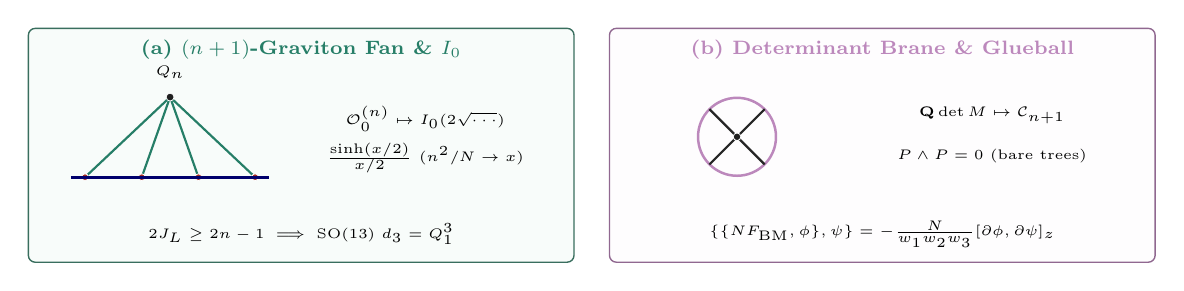
\begin{tikzpicture}[scale=0.90]
  % Left: (n+1)-spoke Q_n ribbon fan -> Bessel I_0 & sinh(x/2)/(x/2)
  \begin{scope}[shift={(-4.10,0)}]
    \draw[rounded corners=2.5pt, draw=PineGreen!65!black, fill=PineGreen!2.5, line width=0.5pt] (-3.85,-1.65) rectangle (3.85,1.65);
    \node[font=\scriptsize\bfseries, text=PineGreen!85!black] at (0,1.35) {(a) $(n+1)$-Graviton Fan \& $I_0$};
    \coordinate (qn) at (-1.85,0.68);
    \foreach \idx/\xx in {1/-3.05, 2/-2.25, 3/-1.45, 4/-0.65} {
      \coordinate (sp\idx) at (\xx,-0.45);
      \draw[prop, PineGreen!85!black] (qn)--(sp\idx);
      \filldraw[vbiv] (sp\idx) circle (0.048cm);
    }
    \draw[line width=1.1pt, draw=NavyBlue!85!black] (-3.25,-0.45)--(-0.45,-0.45);
    \filldraw[v0] (qn) circle (0.056cm) node[above=1pt, font=\tiny] {$Q_n$};
    \node[font=\tiny] at (1.75, 0.38) {$\mathcal{O}_0^{(n)} \mapsto I_0(2\sqrt{\cdots})$};
    \node[font=\tiny] at (1.75,-0.18) {$\frac{\sinh(x/2)}{x/2}$ ($n^2/N\to x$)};
    \node[font=\tiny] at (0,-1.25) {$2J_L \ge 2n-1 \implies \SO(13)\ d_3 = Q_1^3$};
  \end{scope}

  % Right: Determinant brane & bulk glueball kernel
  \begin{scope}[shift={(4.10,0)}]
    \draw[rounded corners=2.5pt, draw=Plum!65!black, fill=Plum!2.5, line width=0.5pt] (-3.85,-1.65) rectangle (3.85,1.65);
    \node[font=\scriptsize\bfseries, text=Plum!85!black] at (0,1.35) {(b) Determinant Brane \& Glueball};
    \coordinate (dc) at (-2.05,0.12);
    \draw[prop, Plum!85!black, line width=0.9pt] (dc) circle (0.55cm);
    \draw[prop] (dc)--++( 0.39, 0.39); \draw[prop] (dc)--++(-0.39, 0.39);
    \draw[prop] (dc)--++(-0.39,-0.39); \draw[prop] (dc)--++( 0.39,-0.39);
    \filldraw[v0] (dc) circle (0.054cm);
    \node[font=\tiny] at (1.55, 0.42) {$\mathbf{Q}\det M \mapsto \mathcal{C}_{n+1}$};
    \node[font=\tiny] at (1.55,-0.15) {$P\wedge P = 0$ (bare trees)};
    \node[font=\tiny] at (0,-1.25) {$\{\{NF_{\mathrm{BM}},\phi\},\psi\} = -\frac{N}{w_1 w_2 w_3}[\partial\phi,\partial\psi]_z$};
  \end{scope}
\end{tikzpicture}
\caption{All-order $\mathcal{N}=4$ twisted holography mechanisms of Theorem~\ref{thm:holography-allorder}: (a)~$(n+1)$-spoke fan isolating $Q_n$ on $\mathcal{O}_0^{(n)}$ (Bessel $I_0$), nonplanar $\frac{\sinh(x/2)}{x/2}$ handles, and the $2J_L \ge 2n-1$ spin bound; (b)~giant-graviton determinant brane $\det M$ and bulk $P\wedge P=0$ evasion via the twice-derived glueball kernel.}
\label{fig:holography-visual}
\end{figure}

% ============================================================================
\section{Turnkey Operational Recipe, Post-\texttt{9e833c8} Evaluation, and Five-Paper Roadmap}
\label{sec:conclusion}
% ============================================================================

We conclude with a turnkey practitioner recipe for evaluating multi-loop holomorphic and holomorphic--topological Feynman diagrams, anomalies $O_n$, and loop-corrected supercharges $Q_n$, followed by a critical scientific assessment of the remaining scaling walls beyond the \texttt{9e833c8} (\texttt{80/100}) milestone~\cite{Repo9e833c8} and the five-paper publication roadmap of the program.

\subsection{Operational Four-Step Recipe for \texorpdfstring{$(H,T)$}{(H,T)} Feynman Diagrams, \texorpdfstring{$Q_n$}{Q\_n}, and \texorpdfstring{$O_n$}{O\_n}}
\label{subsec:operational-recipe}

\begin{summaryblock}{Operational Four-Step Recipe for Multi-Loop Twisted Amplitudes, Anomalies, and Supercharges}
Given a supersymmetric gauge, Chern--Simons, or supergravity twist on $X = \RR^T\times\C^H$ ($D := H+T$):
\begin{itemize}[leftmargin=*]
  \item \textbf{Step~1 (Pure-spinor twist class and universal selection gates).} Read off $(H,T)$ and the BV target class (CS, $BF$, $U\sslash\fg$, BCOV, or $11\mathrm{D}$ $E(5|10)$) from Background Card~6.4 (\S\ref{subsec:esw-taxonomy}). Apply the zero-cost vanishing gates before generating graphs: if $T \ge 2$ ($\rho_n(M)^{\wedge T} = 0$), bulk loops vanish for all $n \ge 1$; if $T = 1$, odd loop orders vanish ($O_{2m+1} = Q_{2m+1} = 0$); in $BF$ and $U\sslash\fg$, bulk QME obstructions terminate at one loop ($O_{n\ge 2} = 0$, $O_1 = -I^{\mathrm{phys}}_{d+2}$); and on $\C^{2|3}$, $Q_n\mathcal{O} = 0$ whenever $2J_L(\mathcal{O}) < 2n-1$.

  \item \textbf{Step~2 (Admissible $D$-Laman / product-forest enumeration and IEC network setup).} Enumerate connected $n$-loop graphs obeying $|I| = Dn+1$, $|V| = (D-1)n+2$, and $(D-1)|I_S| \le D|V_S|-D-1$ (or marked product forests on $\C^2$ with $|E| = 2n+1$ and cycle-free $\Gamma\setminus\{A,B\}$). Form the grounded conductance Laplacian $\Lambda^{uv}(t)$, Symanzik resistance matrix $M_{rs}(t)$, Ohm currents $y^e{}_{\mathsf{a}}(t;\lambda)$, and projective $(|I|-1)$-form $\Omega_\Gamma$~\eqref{eq:sec3-omega-gamma-derived}.

  \item \textbf{Step~3 (Exact Kron / Ohm reduction and period or cube-series evaluation).} Eliminate series/parallel chains, unsourced stars $\mathrm{Y}_0$ (class $\mathrm{B}\supsetneq\mathrm{SP}$), or post-order forest leaves ($\le 3$ retained neighbors; $3$-terminal Markov contact $\langle\xi^2\rangle = \frac{1}{2G}$ at $T=1$; reciprocal inversion $35 \to 15$ on $6$-loop $K_5$). Evaluate the reduced core via closed $\theta(n_1,n_2,n_3)$ determinants~\eqref{eq:theta-closed-both}, fixed-core IBP / parametric annihilators ($W_n$ odd zetas, $K_5$ through $q=9$, $5{,}054$ $T=1$ half-integer periods, $200/200$ five-loop forests incl.\ $K_{3,3}+e$), or $\tau_\Gamma n!$ MST midpoint cube series with $(2n+1)\times(2n+1)$ determinant drop~\eqref{eq:augmented-det-drop}.

  \item \textbf{Step~4 (Lie--Vogel, open-color commutator, and $\eta_v$-cohomology assembly).} Contract color and kinematic factors: in open-color gauge-matter products, apply $[t_A,t_B] - \ii C^C{}_{AB}t_C \equiv 0$ and closed $6$-current Stokes reduction~\eqref{eq:closed-6current-form} to cancel $\zeta(3)$ across all $\deg\Wb \ge 3$ and input derivative jets; in CS/SUGRA QME obstructions, project onto $\eta_v$-invariant local cochains $V_{\mathrm{ht}}$ and evaluate Vogel ladder traces $m_k,n_k$ or Chevalley invariants ($5\mathrm{D}$ $\bigoplus_{\substack{u\\\mathrm{ideals}}}\fsl_{N_u}$ \& $i_4$, $9\mathrm{D}$ $\fsl_{2,3}$, $10\mathrm{D}$ GS, $11\mathrm{D}$ $-\frac{63g}{256\pi^{10}}$); in local operator rings, retain untouched spectator colors and compute the spectral-sequence page $E_{r+1} = H(E_r, d_r)$.
\end{itemize}
\end{summaryblock}

\subsection{Critical Scientific Assessment and Open Frontiers Beyond \texttt{9e833c8}}
\label{subsec:open-frontiers}

Commits \texttt{446559e..9e833c8}~\cite{Repo9e833c8} resolved five major bottlenecks from earlier snapshots: (i)~evaluating the $17$-period five-loop $K_{3,3}+e$ forest residual to $\frac{1187-816\zeta(3)}{435456000}$ and completing all $200/200$ five-loop $\C^2$ product forests; (ii)~proving representation-commutator $\zeta(3)$ cancellation across all open-color $\deg\Wb \ge 3$ products, the $324$-matching $4$-loop $\ghb^2$ product, and arbitrary simultaneous input jets; (iii)~proving fixed-core de~Rham stabilization, the sharp $W_n$ span for $q \ge \max(3,n-1)$, $73$ guarded $q=9$ $K_5$ orbits, $5{,}054$ $T=1$ half-integer periods, $3$-terminal Markov locality, and $92$ five-loop $\C^3$ polynomials; (iv)~establishing the $14$-twist $O_1 = -I^{\mathrm{phys}}_{d+2}$ match and $9\mathrm{D}$ HT CS $\fsl_2,\fsl_3$-sole quantization; and (v)~fixing $\eps_2 = -1$, all $55$ \texttt{tadpole(5,0)} moments, $30{,}272$-monomial $\GL(2)$ $J_w=20$ cohomology, and unique rational $6\mathrm{D}$ $\mathcal{N}=(1,0)$ rank-$5$ weights via the spectator-color audit. Four sharp frontiers remain open:
\begin{enumerate}[label=(\arabic*),leftmargin=*]
  \item \textbf{Budzik--Gaiotto $k=2$ meson wall at $\mathcal{O}_0$ and unmarked $5$-loop bulk graphs:} At level $24$ ($\SU(2)$ fortuitous class $\mathcal{O}_0$), $\dim V_{T,-5} = 1.06\times 10^{12}$ ($\ge 60\,\mathrm{TB}$ RAM vs.\ $153$ $\SU(2)$ cochains) requires homological perturbation transfer---contracting acyclic free pairs onto free cohomology $H^\bullet(Q_{\mathrm{free}})$ prior to assembling the cubic boundary differential. Among unmarked bulk graphs, $12$ $D=2$ five-loop graphs ($6$ $Z_5$, $3$ $K_{3,3}+e$, $3$ $V_7$) and $318$ higher-core \texttt{bulk3(3,5)} graphs await auxiliary-edge / parametric-annihilator closure.

  \item \textbf{Unrestricted $8\mathrm{D}$ order-$3$ rank, $6\mathrm{D}$ $(Q^2)_{\hbar^5}$, and global $11\mathrm{D}$ $\SL_5$ invariants:} Extending the $8\mathrm{D}$ $\fso_5$ order-$3$ functional system from rank $2/12$ to full rank $12/12$, certifying $6\mathrm{D}$ $\mathcal{N}=(1,1)$ $(Q^2)_{\hbar^5}=0$, and compressing global $\SL_5$-invariant $11\mathrm{D}$ targets ($\dim = 1.82\times 10^8$).

  \item \textbf{Higher-order central extensions and $9\mathrm{D}$ $\fsl_3$ at $\hbar^4$:} Testing $\hbar^{\ge 3}$ lifts of $\fso_5\oplus\C\mathbf{1}$ and $G_2..E_8$ in $5\mathrm{D}$ CS and order-$\hbar^4$ QME closure of $9\mathrm{D}$ HT CS on $\fsl_3$.

  \item \textbf{Independent punctured-fivefold bulk $Q_{n\ge 1}$ reproduction and $11\mathrm{D}$ $C_3\wedge X_8(R)$:} Deriving positive-loop $Q_{n\ge 1}$ coefficients directly from regulated bulk BCOV integrals in $N F_{\mathrm{BM}}$ flux, solving the $1$-loop determinant-brane gauge counterterm $R_1$, and testing twisted $C_3\wedge X_8(R)$ Green--Schwarz cancellation against $-\frac{63g}{256\pi^{10}}$ in $11\mathrm{D}$ supergravity (Table~\ref{tab:scorecard}).
\end{enumerate}

\begin{table}[H]
\centering
\scriptsize
\setlength{\tabcolsep}{3.4pt}
\renewcommand{\arraystretch}{1.16}
\begin{tabularx}{\textwidth}{@{}ll>{\raggedright\arraybackslash}X>{\raggedright\arraybackslash}X@{}}
\toprule
\textbf{Paper Track} & \textbf{Status} & \textbf{Verified Scope Through Commit \texttt{9e833c8} (\texttt{80/100})} & \textbf{Immediate Next Action} \\
\midrule
\textbf{Paper I} ($5\mathrm{D}/9\mathrm{D}$ CS) & \textbf{Submission-ready} & $5\mathrm{D}$ $\bigoplus\fsl_{N_u}$, $N=2$, $50$-graph $i_4$, $\fg\oplus\C\mathbf{1}$ (\fivedpdf) $+ 9\mathrm{D}$ $\fsl_{2,3}$ contrast & Submit to \emph{CMP} / \emph{JHEP}; optional $\hbar^4$ check on $9\mathrm{D}$ $\fsl_3$ \\
\textbf{Paper II} (Networks \& Forests) & \textbf{Submission-ready} & $W_n$ span, $K_5$ ($q\le 9$, $6$-loop), $5{,}054$ $T=1$ periods, $200/200$ $5$-loop forests ($K_{3,3}+e$), open-color $\Wb$ \& $6$-current jets & Submit \texttt{notes/methods-paper/} to \emph{CMP} / \emph{CNTP} \\
\textbf{Paper III} ($11\mathrm{D}$ Twisted SUGRA) & \textbf{Submission-ready} & $12$-vertex $1008\pi \mapsto -\frac{63g}{256\pi^{10}}$, rank-$80\to 83$ $\{I_1,I_1\}$ elimination, $T^{2r}\times\C^{5-r}$ routing, Koszul $g$-torsion & Submit \texttt{notes/twisted-sugra-bulk-tests/}; optional $C_3\wedge X_8$ note \\
\textbf{Paper IV} (ESW \& $3\mathrm{D}$--$8\mathrm{D}$ Twists) & \textbf{Near-ready} & $14$-twist $O_1=-I^{\mathrm{phys}}_{d+2}$, $3\mathrm{D}$ $\eps_2=-1$ \& $J_w=20$, $6\mathrm{D}$ $(1,1)$ $Q_4$ \& $(1,0)$ rank-$5$ weights, $\C^3$ $\fso_8$ GS, twistor OPEs & Add $3$-loop Kodaira--Spencer closed exchange for $\fso_8$ \\
\textbf{Paper V} (BCOV \& $\mathcal{N}=4$ Holo) & \textbf{Strong draft} & $4$-loop KS $D_4$, delayed $g=4$ BCOV $\frac{31}{64012032000}$ \& cubic Ward targets, Bessel $I_0$, $\frac{\sinh(x/2)}{x/2}$, $k=2$ mesons, $\det M$, $2J_L\ge 2n-1$ & Punctured bulk $Q_{n\ge 1}$ match; HPL transfer at $\mathcal{O}_0$; $1$-loop brane $R_1$ \\
\bottomrule
\end{tabularx}
\caption{Post-\texttt{9e833c8} readiness scorecard and five-paper publication roadmap of \texttt{holomorphic-topological-feynman-diagrams}.}
\label{tab:scorecard}
\end{table}

\section*{Acknowledgments}
This pedagogically oriented lecture monograph grew out of an effort to make perturbative holomorphic and holomorphic--topological quantum field theory completely self-contained and accessible to readers trained in standard physical quantum field theory, uniting Chern--Simons/AKSZ gauge theory, Lie--Vogel representation theory, Schwinger electrical-network and algebraic de~Rham period geometry, and twisted supergravity/holography within one standardized mathematical convention system.


\appendix
% ============================================================================
\section{Gauge-Group, Spinor, Bispinor, and Electrical Conventions}
\label{app:conventions}
% ============================================================================

This appendix records the gauge-algebra, Euclidean Weyl- and Weinberg--Srednicki four-component spinor, bispinor $\RR^4\cong\C^2$, and $(H,T)$ electrical-network conventions used throughout Sections~\ref{sec:summary-ledger}--\ref{sec:conclusion}, matching~\cite[Ch.~26]{Weinberg} and~\cite{LLC,Repo9e833c8}.

\paragraph{Gauge Lie algebra, matter representations, and covariant derivatives.}
Let $G$ be a compact Lie group with complexified Lie algebra $\fg$ ($\dim_{\C}\fg = d_{\fg}$) and dual $\fg^*$. Uppercase Latin letters $A,B,C,E$ denote basis-independent slots on $\fg$ ($x^A \in \fg$) and $\fg^*$ ($\omega_A \in \fg^*$), related to a basis $(e_m)^A$ and dual $(e^m)_A$ ($m \in \{1,\dots,d_{\fg}\}$) by $x^A = x^m(e_m)^A$ and $\omega_A = \omega_m(e^m)_A$. On semisimple $\fg$, $\kappa_{AB} \in \Sym^2(\fg^*)^{\fg}$ has inverse $\kappa^{AB}$, and Hermitian generators $t_B$ satisfy $[t_B, t_C] = \ii C^A{}_{BC}t_A$ (anti-Hermitian $T_A := \ii t_A$ obey $[T_B, T_C] = -C^A{}_{BC}T_A$). On chiral matter $\cR = \bigoplus_{\substack{s\in\{1,\dots,M\}\\\mathrm{multiplets}}}\cR_s$ ($I,J,K \in \{1,\dots,\dim\cR\}$) with $\mathrm{U}(1)_R$ charges $r_I \in (0,2)$, Euclidean covariant derivatives and field strengths on $\RR^4$ ($g_{\mu\nu} = \delta_{\mu\nu}$) read
\begin{equation}
\label{eq:sum-cov}
\begin{aligned}
(\nabla_\mu\phi)^I &:= \partial_\mu\phi^I + \ii g V_\mu{}^A(t_A)^I{}_J\phi^J, &\qquad
(\nabla_\mu\bar{\phi})_I &:= \partial_\mu\bar{\phi}_I - \ii g V_\mu{}^A\bar{\phi}_J(t_A)^J{}_I,\\
f_{\mu\nu}{}^A &:= \partial_\mu V_\nu{}^A - \partial_\nu V_\mu{}^A - g C^A{}_{BC}V_\mu{}^B V_\nu{}^C, &\qquad
(\nabla_\mu\ghc)^A &:= \partial_\mu\ghc^A - g C^A{}_{BC}V_\mu{}^B\ghc^C,
\end{aligned}
\end{equation}
bridging directly to the differential-form connection $A^{(1)} = A^{(1)A}T_A$ ($\delta_\epsilon A^{(1)A} = -(\dd_\nabla\epsilon)^A$) of Section~\ref{subsec:cs-aksz-lecture} via $A^{(1)A}|_{4\mathrm{D}} = g V_\mu{}^A\dd x^\mu$, $f^A{}_{BC} = -C^A{}_{BC}$, and $\epsilon^A = -g\ghc^A$ ($s A^{(1)A} = -(\dd_\nabla\epsilon)^A = g(\nabla_\mu\ghc)^A\dd x^\mu$).

\paragraph{Euclidean Weyl spinors and Weinberg--Srednicki four-component Majorana spinors.}
Under $\Spin(4) \cong \SU(2)_+ \times \SU(2)_-$, chiral spinors $S_+ \cong \C^2$ ($a,b \in \{+,-\}$) and antichiral spinors $S_- \cong \C^2$ ($\dot{a},\dot{b} \in \{\dot{+},\dot{-}\}$) carry $\eps^{+-} = -\eps^{-+} = +1 = -\eps_{+-} = \eps_{-+}$ and $\eps^{\dot{+}\dot{-}} = -\eps^{\dot{-}\dot{+}} = +1 = -\eps_{\dot{+}\dot{-}} = \eps_{\dot{-}\dot{+}}$, raising and lowering via $\psi^a = \eps^{ab}\psi_b$, $\psi_b = \eps_{bc}\psi^c$, $\bar{\psi}^{\dot{a}} = \eps^{\dot{a}\dot{b}}\bar{\psi}_{\dot{b}}$, and $\bar{\psi}_{\dot{b}} = \eps_{\dot{b}\dot{c}}\bar{\psi}^{\dot{c}}$.

With $(\sigma^\mu)_{a\dot{b}} := (-\ii\mathbf{1}_2, \sigma_1, \sigma_2, \sigma_3)$ and $(\bar{\sigma}^\mu)^{\dot{a}b} := (-\ii\mathbf{1}_2, -\sigma_1, -\sigma_2, -\sigma_3)$, $(\sigma^\mu)_{a\dot{c}}(\bar{\sigma}^\nu)^{\dot{c}b} + (\sigma^\nu)_{a\dot{c}}(\bar{\sigma}^\mu)^{\dot{c}b} = -2\delta^{\mu\nu}\delta_a{}^b$. In four-component Majorana notation ($\alpha,\beta \in \{1,2,3,4\}$), $\lambda_\alpha{}^A := (\lambda_a{}^A, \bar{\lambda}^{\dot{a}A})_\alpha$, $C^{\alpha\beta} := \diag(\eps^{ab}, \eps_{\dot{a}\dot{b}})^{\alpha\beta} = -C_{\alpha\beta}$, $\bar{\lambda}^{\alpha A} := \lambda_\beta{}^A C^{\beta\alpha}$, $(\gamma^\mu)_\alpha{}^\beta := \bigl(\begin{smallmatrix}0 & \ii(\sigma^\mu)_{a\dot{b}}\\ \ii(\bar{\sigma}^\mu)^{\dot{a}b} & 0\end{smallmatrix}\bigr)$, and $(\gamma_5)_\alpha{}^\beta := \diag(\mathbf{1}_2, -\mathbf{1}_2)_\alpha{}^\beta$ satisfy $\{\gamma^\mu, \gamma^\nu\} = 2g^{\mu\nu}\mathbf{1}_4$.

\paragraph{Bispinor coordinates on $\RR^4\cong\C^2$ and self-dual curvature.}
Setting $x^{a\dot{a}} := x^\mu(\bar{\sigma}_\mu)^{\dot{a}a}$ and $\partial_{a\dot{a}} := (\sigma^\mu)_{a\dot{a}}\partial_\mu = -2\partial/\partial x^{a\dot{a}}$ gives
\begin{equation}
\label{eq:z-coords}
\begin{aligned}
x^{+\dot{+}} &= -(x^3 + \ii x^0), & x^{+\dot{-}} &= -(x^1 + \ii x^2), &
x^{-\dot{+}} &= -(x^1 - \ii x^2), & x^{-\dot{-}} &= x^3 - \ii x^0,\\
\partial_{+\dot{+}} &= \partial_3 - \ii\partial_0, & \partial_{+\dot{-}} &= \partial_1 - \ii\partial_2, &
\partial_{-\dot{+}} &= \partial_1 + \ii\partial_2, & \partial_{-\dot{-}} &= -\partial_3 - \ii\partial_0,
\end{aligned}
\end{equation}
with $\Omega := 2\,\dd x^{+\dot{+}}\wedge\dd x^{+\dot{-}}$, $\dbar := \frac{1}{2}\dd x^-_{\dot{a}}\partial_-{}^{\dot{a}}$, $V_{a\dot{a}}{}^A := (\sigma^\mu)_{a\dot{a}}V_\mu{}^A$, $V^{\ddagger a\dot{a}}{}_A := -\frac{1}{2}(\bar{\sigma}_\mu)^{\dot{a}a}V^{\mu\ddagger}{}_A$, and $f_{++}{}^A := \partial_{+\dot{a}}V_+{}^{\dot{a}A} - \frac{g}{2}C^A{}_{BC}V_{+\dot{a}}{}^B V_+{}^{\dot{a}C}$.

\begin{proposition}[Bispinor Laplacian, volume form, and gaugino--ghost soldering~{\cite{LLC}}]
\label{prop:spinor-soldering}
On $\RR^4 \cong \C^2$: (1)~$\partial_{a\dot{a}}(x^{b\dot{b}}) = -2\delta_a{}^b\delta_{\dot{a}}{}^{\dot{b}}$, $-\nabla^2 = \partial_{+\dot{a}}\partial_-{}^{\dot{a}}$, and $\Omega\wedge\dd x^{-\dot{+}}\wedge\dd x^{-\dot{-}} = -8\,\dd^4x$; (2)~specializing $Q_\xi V_\mu{}^A = -\xi^b(\sigma_\mu)_{b\dot{c}}\bar{\lambda}^{\dot{c}A}$ to $\xi_0{}^b = \delta^b{}_-$ yields $(s_{\mathrm{BRST}}+Q_-)V_{+\dot{a}}{}^A = (\nabla_{+\dot{a}}\ghc)^A - 2\bar{\lambda}_{\dot{a}}{}^A$ and $Q_- V_{-\dot{a}}{}^A = 0$.
\end{proposition}

\begin{proof}
Contracting $(\sigma^\mu)_{a\dot{a}}(\bar{\sigma}_\mu)^{\dot{b}b} = -2\delta_a{}^b\delta_{\dot{a}}{}^{\dot{b}}$ and expanding~\eqref{eq:z-coords} proves~(1); $Q_\xi V_{a\dot{a}}{}^A = 2\xi_a\bar{\lambda}_{\dot{a}}{}^A$ evaluated at $\xi_{0,+}=-1, \xi_{0,-}=0$ proves~(2).
\end{proof}

\paragraph{Electrical-network incidence, cycle, and Kirchhoff cotree/tree duality.}
Let $\Gamma = (V,I)$ be a connected oriented multigraph of loop number $n = |I|-|V|+1$ with resistance tensor $R_{ef}(t) = t_e\delta_{ef}$ and conductance tensor $G^{ef}(t) = t_e^{-1}\delta^{ef}$ ($t_e > 0$). Fix a root vertex $v_0 \in V$ ($|V|-1$ ungrounded vertices $u,w \in V\setminus\{v_0\}$) and a spanning tree $T_0 \subset I$ whose $n$ complementary chords $c_1,\dots,c_n \in I\setminus T_0$ define fundamental cycles $C_r{}^e \in \{-1,0,+1\}$.

\begin{proposition}[Orthogonal cut--cycle decomposition and Kirchhoff matrix-tree/cotree identity~{\cite{Mathews,WW24,Repo9e833c8}}]
\label{prop:kirchhoff-duality}
Let $B^u{}_e \in \{-1,0,+1\}$ be the grounded vertex--edge incidence matrix, $L^{uw}(t) := B^u{}_e G^{ef}(t)B^w{}_f$ the grounded conductance Laplacian, and $M_{rs}(t) := C_r{}^e R_{ef}(t)C_s{}^f$ the cycle-resistance matrix in any $\ZZ$-basis of $H_1(\Gamma;\ZZ)$. Then:
\begin{enumerate}[label=(\arabic*),leftmargin=*]
  \item $B^u{}_e C_r{}^e = 0$ identically, and for every conserved source $\lambda^u{}_{\mathsf{a}}$ ($\lambda^{v_0}{}_{\mathsf{a}} = -\sum_{\substack{u\neq v_0\\\mathrm{ungrounded}}}\lambda^u{}_{\mathsf{a}}$) there exists a unique current $y^e{}_{\mathsf{a}}(t,\lambda) = G^{ef}(t)B^u{}_f(L^{-1})_{uw}(t)\lambda^w{}_{\mathsf{a}}$ obeying $B^u{}_e y^e{}_{\mathsf{a}} = \lambda^u{}_{\mathsf{a}}$ and $C_r{}^e R_{ef}(t)y^f{}_{\mathsf{a}} = 0$.

  \item Across all spanning trees $T \subset \Gamma$, cotree cycle determinants and grounded conductance determinants coincide:
  \begin{equation}
  \label{eq:kirchhoff-tree-cotree}
  U_\Gamma(t) := \det M(t) = \sum_{\substack{T\subset\Gamma\\\mathrm{spanning\ trees}}}\prod_{\substack{e\in I\setminus T\\\mathrm{cotree\ chords}}}t_e = \left(\prod_{\substack{e\in I\\\mathrm{all\ edges}}}t_e\right)\det L(t).
  \end{equation}
\end{enumerate}
\end{proposition}

\begin{proof}
In~(1), every closed cycle $r$ enters and leaves each vertex $u$ an equal number of times, giving $B^u{}_e C_r{}^e = 0$; positive-definiteness of $R_{ef}(t)$ on $\RR^{|I|}$ splits $\RR^{|I|} = \im(G B^\dagger) \oplus_R \im(C^\dagger)$, making $y^e{}_{\mathsf{a}} = G^{ef}B^u{}_f(L^{-1})_{uw}\lambda^w{}_{\mathsf{a}}$ the unique simultaneous solution of $B y = \lambda$ and $C R y = 0$. In~(2), Cauchy--Binet on $M = C R C^\dagger$ sums $(\det C|_{I\setminus T})^2\prod_{\substack{e\notin T\\\mathrm{cotree}}}t_e$ over $|I\setminus T| = n$ subsets, where unimodularity gives $(\det C|_{I\setminus T})^2 = 1$ on spanning cotrees and $0$ otherwise; similarly, Cauchy--Binet on $L = B G B^\dagger$ gives $\det L = \sum_{\substack{T\\\mathrm{trees}}}\prod_{\substack{e\in T\\\mathrm{tree}}}t_e^{-1}$, and multiplying by $\prod_{\substack{e\in I\\\mathrm{edges}}}t_e$ yields~\eqref{eq:kirchhoff-tree-cotree}.
\end{proof}

% ============================================================================
\section{Five-Loop Benchmark Ledger, Spectator-Color Audit, and Literature Errata}
\label{app:periods-errata}
% ============================================================================

This second appendix records key quantitative tables supporting Sections~\ref{sec:schwinger-periods-k5}--\ref{sec:sugra-bcov-holo}: (1)~the five-loop $\C^2$ forest and $\C^3$ \texttt{bulk3} benchmark constants; (2)~the complete scope ledger of the spectator-color audit; and (3)~six concrete published/preprint formula errata caught by exact rational and multi-prime modular verification~\cite{Repo9e833c8}.

\subsection{Five-Loop Forest and \texorpdfstring{$\C^3$}{C\^3} Bulk Period Benchmarks}
\label{subsec:app-fiveloop-ledger}

\begin{table}[H]
\centering
\scriptsize
\setlength{\tabcolsep}{4pt}
\renewcommand{\arraystretch}{1.18}
\begin{tabularx}{\textwidth}{@{}ll>{\raggedright\arraybackslash}X@{}}
\toprule
\textbf{Topology / Family} & \textbf{Space \& Pole $q$} & \textbf{Exact Certified Value / Census Breakdown} \\
\midrule
$K_{3,3}+e$ forest $(1,0;2,1;-3,-1)$ & $\C^2$ ($n=5, q=7$) & $\frac{1187 - 816\zeta(3)}{435456000} > 0$ ($17$ annihilators; $+\frac{57527}{106920}\zeta(5)$ cancels) \\
$K_5-e$ physical quartic forest & $\C^2$ ($n=5, q=7,8$) & $16$ bare $+ 468$ current monomials ($1{,}334$ coeffs in $\QQ+\QQ\zeta(3)+\QQ\zeta(5)$) \\
All $200$ five-loop product forests & $\C^2$ ($n=5$, $2{,}200$ spinors) & $10$ zero bare ($10/10$ nonzero currents), $107\in\QQ$, $77\in\QQ+\QQ\zeta(3)$, $6$ with $\zeta(5)$ \\
\texttt{prism} \& $K_{3,3}$ $T=1$ completion & $\RR\times\C$ ($n=4, q\le\frac{11}{2}$) & $5{,}054$ half-integer periods; $K_{\mathrm{prism}}=\frac{311}{630}\pi^2-\frac{17}{360}\pi^4$; $K_{K_{3,3}}\equiv 0$ \\
\texttt{bulk3(3,5)} graph $K_{46}$ (\texttt{prism} core) & $\C^3$ ($n=5, q=8$) & $-\frac{61437767}{18517766400000} - \frac{189281}{21432600000}\zeta(3) + \frac{4}{297675}\zeta(5)$ \\
\texttt{bulk3(3,5)} graph $K_{62}$ ($K_4\oplus_2 K_4$) & $\C^3$ ($n=5, q=8$) & $\frac{2804909}{1866590853120} - \frac{9019}{3600676800}\zeta(3) + \frac{29}{27783000}\zeta(3)^2$ (weight-$6$ $\zeta(3)^2$) \\
Guarded interior $K_5$ orbit & $\C^2$ ($n=6, q=9$) & $\frac{1637270809}{3295339407360000} + \frac{50430067}{22884301440000}\zeta(3) - \frac{551}{181621440}\zeta(5)$ ($73$ orbits) \\
\bottomrule
\end{tabularx}
\caption{Representative five- and six-loop certified period evaluations across $\C^2$, $\RR\times\C$, and $\C^3$~\cite{Repo9e833c8}.}
\label{tab:app-fiveloop-ledger}
\end{table}

\subsection{Spectator-Color Audit Scope Table}
\label{subsec:app-spectator-audit}

In the pooled multi-operator contraction module, an original input letter untouched by both operators in a composition \texttt{op2|op1} previously had its functional color summed alone instead of contracted with its input color vector~\cite{Repo9e833c8}. Restoring exact spectator-color and integer color contractions establishes the complete audit status in Table~\ref{tab:spectator-audit}.

\begin{table}[H]
\centering
\scriptsize
\setlength{\tabcolsep}{3.8pt}
\renewcommand{\arraystretch}{1.16}
\begin{tabularx}{\textwidth}{@{}ll>{\raggedright\arraybackslash}X@{}}
\toprule
\textbf{Calculation Sector} & \textbf{Audit Status} & \textbf{Verified Resolution / Consequence} \\
\midrule
$6\mathrm{D}$ $\mathcal{N}=(1,1)$ order-$4$ ($\ghb^5 \to \ghc^5\gamma_1\gamma_2$) & \textbf{Unaffected} & Input and final letter types disjoint; rank-$15/15$ proof stands unchanged \\
$6\mathrm{D}$ $\mathcal{N}=(1,0)$ ($\gamma^\vee\gamma^\vee u \to \gamma^4 u$, $\fsl_2+16\mathrm{F}$) & \textbf{Replaced (Exact $\QQ$)} & $74{,}458$ rational simplex integrals give rank $5/5$: $\kappa = (\frac{1}{2},\frac{1}{2},1,\frac{1}{2},\frac{1}{2})$ \\
$8\mathrm{D}$ $\mathcal{N}=1$ $\fso_5$ order-$2$ ($(\gamma^\vee)^3 \to \gamma^6\gamma^\vee$) & \textbf{Replayed \& Passed} & $12\times 3$ system has rank $3/3$ with $\kappa_2 = (-\frac{1}{2},-1,-\frac{1}{6})$ ($0$ residuals) \\
$8\mathrm{D}$ $\mathcal{N}=1$ $\fso_5$ order-$3$ ($(\gamma^\vee)^4 \to \gamma^8\gamma^\vee$) & \textbf{Replayed ($18/18$)} & All $18$ reverse/mixed compositions match; rank $2/12$, unique all-minus sign ($1/4{,}096$) \\
$3\mathrm{D}$ \texttt{ht3d} / \texttt{qn-ht}, graph kernels, trace anomalies & \textbf{Unaffected} & Separate engines without pooled spectator contraction ($30{,}272$-monomial $J_w=20$ verified) \\
\bottomrule
\end{tabularx}
\caption{Complete scope and resolution ledger of the composed-operator spectator-color audit~\cite{Repo9e833c8}.}
\label{tab:spectator-audit}
\end{table}

\subsection{Six Published and Preprint Formula Errata Caught by Zero-Import Verification}
\label{subsec:app-errata}

\begin{enumerate}[label=\textbf{Erratum~\arabic*.},leftmargin=*]
  \item \textbf{Costello--Dimofte--Gaiotto~\cite{CDG20}, eq.~(5.7):} The printed $3\mathrm{D}$ HT propagator fails $D_{\mathrm{free}}$-closedness away from $0$ ($D_{\mathrm{free}}[\cdots] = \frac{2\tau^2-|z|^2}{2|x|^5}\dd\tau\wedge\dd\bar{z}\wedge\dd z \neq 0$), repaired by restoring the factor-$2$ in $(2\bar{z}\dd\tau - \tau\dd\bar{z})/(8\pi\ii|x|^3)$.

  \item \textbf{Gaiotto--Kulp--Wu~\cite{GKW}, eq.~(3.59) \& HTML eq.~(109):} Eq.~(3.59) differs from eq.~(3.52) by $2\pi^3$, and the printed bitriangle sign/magnitude differs from the direct Gaussian pushforward $I^{\mathrm{GKW}} = -(4\pi)^{-1}K^{\mathrm{htk}}$ ($\eps_2 = -1$, Theorem~\ref{thm:3d-n2-complete}(1)).

  \item \textbf{Wang--Williams~\cite{WW24}, eq.~(22):} Heat-kernel normalization factor-$4$ discrepancy relative to $[D_{\mathrm{free}}, D^*] = -\delta^{\rho\sigma}\partial_{\tau^\rho}\partial_{\tau^\sigma} - 4\delta^{\bar{\jmath}i}\partial_i\dbar_{\bar{\jmath}}$~\eqref{eq:ht-heat-kernel-explicit}.

  \item \textbf{Costello--Li~\cite{CL19}, eq.~(85):} Missing holomorphic derivative factor $\partial A$ in the printed Type~I open-closed coupling.

  \item \textbf{Oh--Zhou, Fig.~12:} Differential-form wedge-commutation sign slip rendering a printed vertex expression zero.

  \item \textbf{Ketov $\mathrm{WZW}_4$ background connection:} Nonvanishing curvature in the stated background connection (Theorem~\ref{thm:ks-bcov}(2)).
\end{enumerate}


\begin{thebibliography}{99}\footnotesize\raggedright\setlength{\itemsep}{1.5pt}\setlength{\parskip}{0pt}

\bibitem{AKSZ97}
M.~Alexandrov, M.~Kontsevich, A.~Schwarz, and O.~Zaboronsky,
\emph{The geometry of the master equation and topological quantum field theory},
Int.\ J.\ Mod.\ Phys.\ A \textbf{12} (1997), 1405--1429, arXiv:hep-th/9502010.

\bibitem{BBH}
G.~Barnich, F.~Brandt, and M.~Henneaux,
\emph{Local BRST cohomology in gauge theories},
Phys.\ Rept.\ \textbf{338} (2000), 439--569, arXiv:hep-th/0002245.

\bibitem{BCOV94}
M.~Bershadsky, S.~Cecotti, H.~Ooguri, and C.~Vafa,
\emph{Kodaira--Spencer theory of gravity and exact results for quantum string amplitudes},
Commun.\ Math.\ Phys.\ \textbf{165} (1994), 311--428, arXiv:hep-th/9309140.

\bibitem{BBKP18}
T.~Bitoun, C.~Bogner, R.~P.~Klausen, and E.~Panzer,
\emph{Feynman integral relations from parametric annihilators},
Lett.\ Math.\ Phys.\ \textbf{109} (2019), 497--564, arXiv:1712.09215.

\bibitem{BSS22}
R.~Bittleston, A.~Sharma, and D.~Skinner,
\emph{Quantizing the non-linear graviton},
Commun.\ Math.\ Phys.\ \textbf{403} (2023), 1543--1609, arXiv:2208.12701.

\bibitem{Bott59}
R.~Bott,
\emph{The stable homotopy of the classical groups},
Ann.\ of Math.\ (2) \textbf{70} (1959), 313--337.

\bibitem{BW23}
P.~Bomans and J.~Wu,
\emph{Unravelling the holomorphic twist: central charges},
JHEP \textbf{04} (2024), 052, arXiv:2311.04304.

\bibitem{BG26}
K.~Budzik and D.~Gaiotto,
\emph{Finite-$N$ BPS Hilbert spaces and Koszul dual D-brane meson complexes},
arXiv:2611.18539 (2026).

\bibitem{BGKWY}
K.~Budzik, D.~Gaiotto, J.~Kulp, J.~Wu, and M.~Yu,
\emph{Feynman diagrams in four-dimensional holomorphic theories and the operatope},
JHEP \textbf{07} (2023), 127, arXiv:2207.14321.

\bibitem{BGKWWY}
K.~Budzik, D.~Gaiotto, J.~Kulp, B.~R.~Williams, J.~Wu, and M.~Yu,
\emph{Semi-chiral operators in 4d $\mathcal{N}=1$ gauge theories},
JHEP \textbf{05} (2024), 245, arXiv:2306.01039.

\bibitem{BK}
K.~Budzik and J.~Kulp,
\emph{Loop corrected supercharges from holomorphic anomalies},
arXiv:2512.07771 (2025).

\bibitem{CDSW}
F.~Cachazo, M.~R.~Douglas, N.~Seiberg, and E.~Witten,
\emph{Chiral rings and anomalies in supersymmetric gauge theory},
JHEP \textbf{12} (2002), 071, arXiv:hep-th/0211170.

\bibitem{CSS13}
S.~Caracciolo, A.~D.~Sokal, and A.~Sportiello,
\emph{Algebraic/combinatorial proofs of Cayley-type identities for derivatives of determinants and pfaffians},
Adv.\ Appl.\ Math.\ \textbf{50} (2013), 474--594, arXiv:1105.6270.

\bibitem{Cederwall10}
M.~Cederwall,
\emph{$D=11$ supergravity with manifest supersymmetry},
Mod.\ Phys.\ Lett.\ A \textbf{25} (2010), 3201--3212, arXiv:1001.0112.

\bibitem{ChangLin}
C.-M.~Chang and Y.-H.~Lin,
\emph{Words to describe a black hole},
JHEP \textbf{02} (2023), 109, arXiv:2209.06728.

\bibitem{ChangYin}
C.-M.~Chang and X.~Yin,
\emph{$1/16$ BPS states in $\mathcal{N}=4$ super-Yang--Mills theory},
Phys.\ Rev.\ D \textbf{88} (2013), 106005, arXiv:1305.6314.

\bibitem{Costello}
K.~Costello,
\emph{Renormalization and Effective Field Theory},
Mathematical Surveys and Monographs \textbf{170}, American Mathematical Society (2011).

\bibitem{CostelloNotes}
K.~Costello,
\emph{Notes on supersymmetric and holomorphic field theories in dimensions $2$ and $4$},
Pure Appl.\ Math.\ Q.\ \textbf{9} (2013), 73--165, arXiv:1111.4234.

\bibitem{Costello16}
K.~Costello,
\emph{M-theory in the Omega-background and 5-dimensional non-commutative gauge theory},
arXiv:1610.04144 (2016).

\bibitem{CDG20}
K.~Costello, T.~Dimofte, and D.~Gaiotto,
\emph{Boundary chiral algebras and holomorphic twists},
Commun.\ Math.\ Phys.\ \textbf{399} (2023), 1203--1290, arXiv:2005.00083.

\bibitem{CG18}
K.~Costello and D.~Gaiotto,
\emph{Twisted holography},
arXiv:1812.09257 (2018).

\bibitem{CG2}
K.~Costello and O.~Gwilliam,
\emph{Factorization Algebras in Quantum Field Theory, Vol.~2},
Cambridge University Press (2021).

\bibitem{CL19}
K.~Costello and S.~Li,
\emph{Anomaly cancellation in the topological string},
Adv.\ Theor.\ Math.\ Phys.\ \textbf{24} (2020), 1723--1771, arXiv:1905.09269.

\bibitem{CWY18}
K.~Costello, E.~Witten, and M.~Yamazaki,
\emph{Gauge theory and integrability, I},
ICCM Not.\ \textbf{6} (2018), 46--119, arXiv:1709.09993.

\bibitem{CJS78}
E.~Cremmer, B.~Julia, and J.~Scherk,
\emph{Supergravity theory in $11$ dimensions},
Phys.\ Lett.\ B \textbf{76} (1978), 409--412.

\bibitem{ESW}
C.~Elliott, P.~Safronov, and B.~R.~Williams,
\emph{A taxonomy of twists of supersymmetric Yang--Mills theory},
Selecta Math.\ \textbf{28} (2022), 73, arXiv:2002.10517.

\bibitem{FP24}
V.~E.~Fern\'andez and N.~M.~Paquette,
\emph{Associativity is enough: an all-orders 2d chiral algebra for 4d form factors},
arXiv:2412.17168 (2024).

\bibitem{FPW24}
V.~E.~Fern\'andez, N.~M.~Paquette, and B.~R.~Williams,
\emph{Twisted holography on $\mathrm{AdS}_3\times S^3\times K3$ and the planar chiral algebra},
arXiv:2404.14318 (2024).

\bibitem{GKW}
D.~Gaiotto, J.~Kulp, and J.~Wu,
\emph{Higher operations in perturbation theory},
JHEP \textbf{05} (2025), 230, arXiv:2403.13049.

\bibitem{GWW}
Z.~Gui, M.~Wang, and B.~R.~Williams,
\emph{Higher-dimensional chiral algebras in the Jouanolou model and free-field realization},
arXiv:2510.26608 (2025).

\bibitem{GW18}
O.~Gwilliam and B.~R.~Williams,
\emph{Higher Kac--Moody algebras and symmetries of holomorphic field theories},
Adv.\ Theor.\ Math.\ Phys.\ \textbf{25} (2021), 129--239, arXiv:1810.06534.

\bibitem{HPR25}
F.~Hahner, N.~M.~Paquette, and S.~Raghavendran,
\emph{Higher symmetries in twisted eleven-dimensional supergravity},
arXiv:2506.02246 (2025).

\bibitem{Konishi}
K.~Konishi,
\emph{Anomalous supersymmetry transformation of some composite operators in SQCD},
Phys.\ Lett.\ B \textbf{135} (1984), 439--444.

\bibitem{LLC}
B.~Li, K.~Liu, and C.-M.~Chang,
\emph{Holomorphic Feynman diagrams in four dimensions and the quantum BPS ring},
arXiv:2611.24160 (2026).

\bibitem{LW26}
S.~Li and Z.~Wang,
\emph{Flat-space quantization and higher-genus vertices of minimal BCOV theory},
arXiv:2610.21927 (2026).

\bibitem{Mathews}
J.~Mathews,
\emph{Application of linear network analysis to Feynman diagrams},
Phys.\ Rev.\ \textbf{113} (1959), 381--385.

\bibitem{MSV11}
R.~L.~Mkrtchyan, A.~N.~Sergeev, and A.~P.~Veselov,
\emph{Casimir eigenvalues for universal Lie algebra},
J.\ Math.\ Phys.\ \textbf{53} (2012), 102106, arXiv:1105.0115.

\bibitem{Panzer15}
E.~Panzer,
\emph{Algorithms for the symbolic integration of hyperlogarithms with applications to Feynman integrals},
Comput.\ Phys.\ Commun.\ \textbf{188} (2015), 148--166, arXiv:1403.3385.

\bibitem{RSW21}
S.~Raghavendran, I.~Saberi, and B.~R.~Williams,
\emph{Twisted eleven-dimensional supergravity},
Commun.\ Math.\ Phys.\ \textbf{402} (2023), 1103--1166, arXiv:2111.03049.

\bibitem{Repo9e833c8}
B.~Li,
\emph{Exact network reduction, multi-loop periods, and anomaly classification in holomorphic-topological Feynman diagrams},
research archive \texttt{holomorphic-topological-feynman-diagrams} through commit \texttt{9e833c8} (2026).

\bibitem{SW}
I.~Saberi and B.~R.~Williams,
\emph{Twisted characters and holomorphic symmetries},
Lett.\ Math.\ Phys.\ \textbf{110} (2020), 2779--2853, arXiv:1906.04221.

\bibitem{Schnetz10}
O.~Schnetz,
\emph{Quantum periods: a census of $\phi^4$-transcendentals},
Commun.\ Number Theory Phys.\ \textbf{4} (2010), 1--48, arXiv:0801.2856.

\bibitem{TT87}
G.~Tian,
\emph{Smoothness of the universal deformation space of compact Calabi--Yau manifolds and its Petersson--Weil metric},
in \emph{Mathematical Aspects of String Theory}, World Scientific (1987), 629--646.

\bibitem{Wang}
M.~Wang,
\emph{Feynman graph integrals on $\mathbb{C}^d$},
arXiv:2401.08113 (2025).

\bibitem{WW24}
M.~Wang and B.~R.~Williams,
\emph{On the renormalization and quantization of topological-holomorphic field theories},
arXiv:2407.08667 (2026).

\bibitem{Weinberg}
S.~Weinberg,
\emph{The Quantum Theory of Fields, Vol.~III: Supersymmetry},
Cambridge University Press (2000).

\bibitem{Williams}
B.~R.~Williams,
\emph{Renormalization for holomorphic field theories},
Commun.\ Math.\ Phys.\ \textbf{374} (2020), 1693--1742, arXiv:1809.02661.

\bibitem{Witten89}
E.~Witten,
\emph{Quantum field theory and the Jones polynomial},
Commun.\ Math.\ Phys.\ \textbf{121} (1989), 351--399.

\end{thebibliography}

\end{document}
